%\includeonly{eq, num, time}
%\includeonly{num,eqice}

\documentclass[11pt,twoside,letterpaper]{article}
\usepackage{latexsym,fancyheadings}
%\usepackage[pdftex]{graphicx}
\usepackage{graphicx}
\usepackage{amsmath}
\usepackage{lmodern}
\usepackage[T1]{fontenc}
\usepackage{textcomp}
\usepackage{hyperref}
%\usepackage{draftcopy}
%\documentstyle[12pt]{report}
%\flushbottom
\setlength{\oddsidemargin}{.0 in}
\setlength{\evensidemargin}{.0 in}
\setlength{\headheight}{0pt}
\setlength{\topmargin}{-.5 in}
\setlength{\headsep}{0pt}
\setlength{\textheight}{9.5 in}
\setlength{\textwidth}{6.5 in}
\setlength{\headrulewidth}{0pt}
%\cfoot{\rm II-\thepage} % page number
\cfoot{\rm \thepage} % page number
\lhead{}
\rhead{}
%\setlength{\oddsidemargin}{0pt}
%\setlength{\headheight}{0pt}
%\setlength{\topmargin}{0pt}
%\setlength{\headsep}{0pt}
%\setlength{\textheight}{9in}
%\setlength{\textwidth}{6.5in}
%\setlength{\oddsidemargin}{0pt}
%\setlength{\oddsidemargin}{0pt}
\newenvironment{klist}{\begin{list}{}{%
    \setlength{\labelwidth}{1.4cm}%
    \addtolength{\leftmargin}{.65cm}%
    \setlength{\itemindent}{.0cm}}}{\end{list}}
\newenvironment{khlist}{\begin{list}{}{%
    \setlength{\itemsep}{0cm}%
    \setlength{\parsep}{0cm}%
    \setlength{\labelsep}{.7cm}%
    \setlength{\labelwidth}{.5cm}%
    \setlength{\leftmargin}{1.3cm}%
    \setlength{\itemindent}{1cm}}}{\end{list}}
\newcommand{\code}[1]{\mbox{\bf#1}}
\newcommand{\kitem}[1]{\item[\bf#1\hfill]}
\newcommand{\pder}[2]{\frac{\partial #1}{\partial #2}}
\def\CC{{C\hspace{-.05em}\raisebox{.4ex}{\tiny\bf ++}}}
%\usepackage[pdftex,
%   pdftitle={Technical Manual for a Coupled Sea-Ice/Ocean
%   Cirulation Model (Version 3)},
%   pdfauthor={Katherine S. Hedstr\"om},
%   pdfkeywords={ROMS, ocean, model},
%   plainpages=false
% ]{hyperref}
\begin{document}

\pagestyle{empty}
\centerline{\hfill OCS Study BOEM 2012-0xx}
\vspace {2 cm}
\begin{center}
  {\LARGE DRAFT Technical Manual for a Coupled Sea-Ice/Ocean \\ Circulation
   Model (Version 4)  }
\end{center}
\vspace {2 cm}
\begin{center}
  Katherine S. Hedstr\"{o}m \\ Arctic Region Supercomputing Center
  \\ University of Alaska Fairbanks
\end{center}
\vspace {2 cm}
\begin{center}
  U.S.\ Department of the Interior \\ Bureau of Ocean Energy
  Management \\
  Herndon, Virginia \\ \mbox{} \\ Contract No.\ M10PC00116
\end{center}
\newpage
\centerline{\hfill OCS Study BOEM 2012-0xx}
\vspace {2 cm}
\begin{center}
  {\LARGE DRAFT Technical Manual for a Coupled Sea-Ice/Ocean \\ Circulation
   Model (Version 4)  }
\end{center}
\vspace {2 cm}
\begin{center}
  Katherine S. Hedstr\"{o}m \\ Arctic Region Supercomputing Center
  \\ University of Alaska Fairbanks
\end{center}
\vspace {2 cm}
\centerline{June 2013}
\vfill


This study was funded by the Alaska Outer Continental Shelf Region
of the Bureau of Ocean Energy Management, U.S.\ Department of the
Interior, Herndon, Virginia, through Contract
{\bf M10PC00116} with Rutgers University, Institute of Marine
and Coastal Sciences.

\vspace {1 cm}
The opinions, findings, conclusions, or recommendations expressed in
this report or product are those of the authors and do not
necessarily reflect the views of the U.S.\ Department of the
Interior, nor does mention of trade names or commercial products
constitute endorsement or recommendation for use by the Federal
Government.
\setcounter{page}{0}
This document was prepared with \LaTeX\, xfig, and inkscape.

\mbox{  }
\begin{center}
\bf \LARGE Acknowledgments
\end{center}

The ROMS model is descended from the SPEM and SCRUM models, but has
been entirely rewritten by Sasha Shchepetkin, Hernan Arango and John
Warner, with many, many other contributors. I am indebted to every one
of them for their hard work.

Bill Hibler first came up with the viscous-plastic rheology we are
using. Paul Budgell has rewritten the dynamic sea-ice model, improving
the solution procedure and making the water-stress term implicit in time,
then changing it again to use the elastic-viscous-plastic rheology of
Hunke and Dukowicz. I am very grateful that he is allowing us to use
his version of the code. The sea-ice thermodynamics is derived from
Sirpa H\"akkinen's implementation of the Mellor-Kantha scheme. She was
kind enough to allow Paul and I to start with her code.

Thanks to the internet community for providing great tools like Perl,
Python, cpp, svn, git, and gmake to aid in software development (and to make
it more fun).

This work was supported in part by a grant of HPC resources from the
Arctic Region Supercomputing Center.

Development and testing of the ROMS model has been funded by many,
including the USGS Coastal and Marine Program, the Office of Naval
Research, the National Ocean Partnership Program...

\vspace{\fill}
UNIX is a registered trademark of the Open Group.

Cygwin is a registered trademark of Red Hat, Inc.


\vfil\break
\begin{abstract}
The Regional Ocean Modeling System (ROMS), authored by many, most
notably Sasha Shchepetkin, is one approach to regional and basin-scale ocean
modeling. This user's manual for ROMS describes the model equations
and algorithms, as well as additional user configurations necessary
for specific applications. ROMS itself has now branched out as
well---the version described here is that available through the
myroms.org svn site with modifications to include sea ice and other
changes. This sea ice branch is also available at github.com.

\end{abstract}

%\newpage
\pagestyle{fancyplain}
\setcounter{page}{1}
\pagenumbering{roman}
\tableofcontents
\newpage
%\setcounter{page}{5}
\listoffigures
%\newpage
\listoftables
%\bibliographystyle{plain}
\bibliographystyle{plainnat}
\pagenumbering{arabic}
\setcounter{page}{1}
\section{Introduction}
\label{Intro}
This user's manual for the Regional Ocean Modeling System (ROMS)
describes the model equations and algorithms, as well as
additional user configurations necessary for specific applications.
This manual also describes the sea-ice model
that we are using (Budgell \cite{Budgell05}).

The principle attributes of the model are as follows:
\begin{klist}
\kitem{General} \mbox{}
\begin{itemize}
  \item Primitive equations with potential temperature, salinity, and an
equation of state.
  \item Hydrostatic and Boussinesq approximations.
  \item Optional third-order upwind advection scheme.
  \item Optional Smolarkiewicz advection scheme for tracers
    (potential temperature, salinity, etc.).
% \item Second-moment conservation.
  \item Optional Lagrangian floats.
  \item Option for point sources and sinks.
\end {itemize}
\kitem{Horizontal} \mbox{}
\begin{itemize}
  \item Orthogonal-curvilinear coordinates.
  \item Arakawa C grid.
  \item Closed basin, periodic, prescribed, radiation, and
    gradient open boundary conditions.
  \item Masking of land areas.
  \item Early version of nesting.
\end {itemize}
\kitem{Vertical} \mbox{}
\begin{itemize}
  \item $\sigma$ (terrain-following) coordinate.
  \item Free surface.
  \item Tridiagonal solve with implicit treatment of vertical
    viscosity and diffusivity.
\end {itemize}
\kitem{Ice} \mbox{}
\begin{itemize}
  \item Hunke and Dukowicz elastic-viscous-plastic dynamics.
  \item Mellor-Kantha thermodynamics.
  \item Orthogonal-curvilinear coordinates.
  \item Arakawa C grid.
  \item Smolarkiewicz advection of tracers.
%  \item Optional ridging scheme.
\end{itemize}
\kitem{Mixing options} \mbox{}
\begin{itemize}
  \item Horizontal Laplacian and biharmonic
    diffusion along constant $s$, $z$ or density
    surfaces.
  \item Horizontal Laplacian and biharmonic viscosity
    along constant $s$ or $z$ surfaces.
  \item Optional Smagorinsky horizontal viscosity and diffusion (but
  not recommended for diffusion).
%  \item Optional Gent and McWilliams \cite{Gent90}, \cite{Gent95} 
%    eddy-induced horizontal mixing.
  \item Horizontal free-slip or no-slip boundaries.
  \item Vertical harmonic viscosity and diffusion with a spatially
    variable coefficient, with options to compute the coefficients
    with Large et al.\ \cite{Large94}, Mellor-Yamada \cite{Mellor74},
    or generic length scale (GLS) \cite{Umlauf2003} mixing schemes.
\end{itemize}
\kitem{Implementation} \mbox{}
\begin{itemize}
  \item Dimensional in meter, kilogram, second (MKS) units.
  \item Fortran 90.
  \item Runs under UNIX, requires the C preprocessor, gnu make, and
  Perl.
  \item All input and output is done in NetCDF \cite{netCDF} (Network
    Common Data Format), requires the NetCDF and NetCDF-fortran
    libraries.
  \item Options include serial, parallel with MPI, and parallel with
  OpenMP.
%  \item Pre- and post-processing graphics package available which
%    uses the NCAR (National Center for Atmospheric Research)
%    graphics libraries.
\end{itemize}
\end{klist}
The above list hasn't changed so very much in the past ten to fifteen
years, but many of the numerical details have changed a great deal.
Examples include consistent temporal averaging of the barotropic
mode to guarantee both exact conservation and constancy preservation
properties for tracers; redefined barotropic pressure-gradient terms
to account for local variations in the density field; vertical
interpolation performed using conservative parabolic splines; and
higher-order, quasi-monotone advection algorithms.

New with this version of the manual is the introduction of nesting
capabilities which requires Matlab for preprocessing.

ROMS also comes with a full suite of advanced data assimilation
routines; these options are beyond the scope of this document.

Chapter \ref{Starting} has some information on getting started with
ROMS.
Chapters \ref{Phys} and \ref{Num} describe the model physics and
numerical techniques and contain information from Shchepetkin and
McWilliams \cite{SS2008b} and Haidvogel et al.\
\cite{Haidvogel07}.
Chapter \ref{Iphys} describes the ice equations and
Chapter \ref{Code} lists the model subroutines and functions.
%Chapter \ref{Progs} describes
%the support programs which are needed to provide ROMS with data files.
As distributed, ROMS is ready to run with a number of example problems.
The process of configuring ROMS for a particular application and
running it is
described in Chapter \ref{Wave}, including a discussion of a few example
applications.
%Chapter \ref{Floats} describes the Lagrangian floats and
%how to use them, including the plotting postprocessor \code{fltplt}.
%Chapter \ref{Plothist} describes Hernan Arango's plotting
%programs \code{cnt}, \code{ccnt}, \code{sec}, and \code{csec}.
%while chapter
%\ref{Userice} describes the ice subroutines and the coupling procedure.

\section{Getting started}
\label{Starting}

\subsection{myroms.org}
\label{Myroms}
Starting off with ROMS is not the easiest thing to do, and it just
seems to be getting more complex as time goes by. There are
some resources, however, beginning with the
electronic home for ROMS users at
\href{http://www.myroms.org}{www.myroms.org}. Go to register,
which gives you access to the subversion server for the code and to
the  discussion forum for all things ROMS. There is also a wiki,
a bug tracking system, and even a developer blog.

The wiki contains parts of this manual, but the nature of wikis is that
they can be more fluid, with more authors, than a static document such
as this. Dave Robertson (robertson@marine.rutgers.edu) is the one to
talk to if you would like to contribute to the wiki.

\subsection{Prerequisites}
As mentioned in Chapter \ref{Intro}, ROMS has some external
requirements. These are:
\begin{itemize}
    \item UNIX or UNIX-like environment, such as
      \href{http://www.redhat.com/services/custom/cygwin/}{Cygwin}.
    \item A Fortran 90 compiler.
    \item The
      \href{http://www.unidata.ucar.edu/software/netcdf/index.html}{NetCDF
      library} compiled with the above compiler, including the
      Fortran 90 interface
      (\href{http://www.unidata.ucar.edu/downloads/netcdf/netcdf-fortran/}{NetCDF-Fortran}
      is now a separate package).
    \item \href{http://subversion.tigris.org}{svn}, the subversion
      revision control software. See Appendix \ref{Svn} and the
      \href{https://www.myroms.org/wiki/index.php/Subversion}{ROMS wiki}.
    \item \href{http://www.gnu.org/software/make/}{Gnu make} version
      3.81 or higher. Appendix \ref{Gmake} contains more than you
      ever wanted to know about this software.
    \item A \href{http://en.wikipedia.org/wiki/C_preprocessor}{C
      preprocessor}---the one from gnu with the \code{-traditional}
      flag works well. See Appendix \ref{Cpp}.
    \item The \href{http://www.perl.org}{Perl} scripting language.
    \item \href{http://www.mathworks.com/products/matlab/}{Matlab} is
      optional, but it is a common tool for pre- and post-processing
      of ROMS files.
\end{itemize}
Make sure you've got the right environment before attempting to
download or compile ROMS. In particular, it's best to download ROMS
using the same environment as will be used when compiling and
running it.

\subsection{Acquiring the ROMS code}
The main ROMS code is available for download via \code{svn} at
\url{https://www.myroms.org/svn/src/}.
The version of the model described in this document is a merger between
ROMS 3.6 and a sea-ice model.
The sea ice code is a branch off a different repository and requires
special access---contact Dave Robertson (as above) for more information.
Alternately, it is available at
\href{https://kshedstrom@github.com/kshedstrom/roms.git}{github.com}
via git.

ROMS comes with several cases all ready to go at the flip
of a switch. Try these out first and get to understand how they
are set up.
    \begin{itemize}
      \item \S\ref{Build} describes how to pick the cases and set up
      the build environment.
      \item \S\ref{Cpp1} lists all the ROMS options that can be
      added to your case.
      \item \S\ref{Functionals} lists the fields which can be
      provided to ROMS via analytic expressions.
      \item \S\ref{ASCII_in} lists the input parameters ROMS reads
      from a text file at run time.
      \item Chapters \ref{Code} and \ref{Wave} are meant to be
      informative for the simple and not-so-simple cases. If that
      isn't the case, please let me know.
    \end{itemize}
In addition to this manual, there are some other ROMS resources:
\begin{itemize}
   \item You may be best served by going to the 
\href{https://www.myroms.org/wiki/}{ROMS wiki} which includes
sections called Getting Started and Tutorials.
   \item Don't be afraid to use the forum. It has everything from
employment opportunities to debugging help. Posting there can get
you help from one of several people, improving your odds of success
over private emails. Registered users get an email once a day about
new postings, so you might have to wait a day (or more) for a reply.
   \item There have been ROMS meetings and classes in which a tutorial
session is included as part of the program.
   \item There are various resources
from these online---I've heard good things about the
\href{http://eros.eas.gatech.edu/ROMS-Tutorial/tutorials.html}{tutorials}
from Manu Di Lorenzo.
\end{itemize}

\subsection{Compiling ROMS}
\label{Build}

\subsubsection{Environment Variables for \code{make}}
\label{make_var}

ROMS has a growing list of choices the user must make about the
compilation before starting the compile process,
set in user-defined variables. Since we now use \code{gnu make}, it is
possible to set the value of these variables in the Unix environment,
rather than necessarily inside the \code{Makefile} (see \S\ref{Gmake}).
The user-definable variables understood by the ROMS \code{makefile} are:
\begin{klist}

\kitem{ROMS\_APPLICATION} Set the \code{cpp} option defining the particular
application. This is used for setting up options inside the code
specific to this application and also determines the name of the
\code{.h} header file for it. This can be either a predefined
case, such as \code{BENCHMARK}, or one of your own, such as \code{NEP5}.

\kitem{MY\_HEADER\_DIR} Sets the path to the user's header file, if
any. It can be left empty for the standard cases, where \code{benchmark.h}
and the like are found in \code{ROMS/Include}, which is already in
the search path. In the case of \code{NEP5}, this is set to
\code{Apps/NEP} where \code{nep5.h} resides.

\kitem{MY\_ANALYTICAL\_DIR} Sets the path to the user's analytic files
described in \S\ref{Functionals}, if any. This can be \code{User/Functionals}
or some other location. I tend to place both the header file and the
functionals in the same directory, one directory per application.

\kitem{MY\_CPP\_FLAGS} Set tunable \code{cpp} options. Sometimes it is desirable
to activate one or more \code{cpp} options to run different variants of the
same application without modifying its header file. If this is the
case, specify each option here using the \code{-D} syntax. Notice that
you need to use the shell's quoting syntax (either single or double
quotes) to enclose the definition if you are using one of the build
scripts below.

%\kitem{NestedGrids} Integer number of grids in the setup, usually 1.

\kitem{Compiler-specific Options} These flags are used by the files
inside the \code{Compilers} directory.
\begin{klist}
  \kitem{USE\_DEBUG} Set this to \code{on} to turn off optimization
and turn on the \code{-g} flag for debugging.

  \kitem{USE\_MPI} Set this if running an MPI parallel job.
  \kitem{USE\_OpenMP} Set this if running an OpenMP parallel job.
  \kitem{USE\_MPIF90} This flag changes the name of the
  Fortran compiler to \code{mpif90}, while
  \code{USE\_MPI} changes the \code{cpp} flags
  for changing the source code. \code{OpenMPI} and others
  provide a shell script called \code{mpif90} for finding the required MPI
  files.
  \kitem{USE\_LARGE}  Some systems support both 32-bit and 64-bit
  options. Select this to get 64-bit addressing, usually used for
  programs needing more than 2 GB of memory on 32-bit systems.
  \kitem{USE\_NETCDF4} Set this if linking against the NetCDF4
  library. If set, ROMS will use \code{nc-config} to locate the
  libraries and module files.
  \kitem{NC\_CONFIG} Set to the \code{nc-config} you wish to use.
  \kitem{NETCDF\_INCDIR} If not using \code{nc-config}, set the
  location of the \code{netcdf.mod} and \code{typesizes.mod} files.
  \kitem{NETCDF\_LIBDIR} The location of the NetCDF library (again,
  when not using \code{nc-config}).
\end{klist}

\kitem{FORT} A shorthand name for the compiler to be used when
selecting which system-compiler file is to be included from the
\code{Compilers} directory. See section \S\ref{Inc_fort} and
\S\ref{make_env}.

\kitem{Local File Options}
\begin{klist}
  \kitem{BINDIR} Directory in which to place the binary executable.
The default is ``\code{.}'', the current directory.

  \kitem{SCRATCH\_DIR} Put the \code{.f90} and the temporary binary files
in a build directory to avoid clutter. The default is \code{Build}
under the top directory. Set it to something else if you want
to keep these files for multiple projects at the same time, each in
their own directory.
\end{klist}
\end{klist}

\subsubsection{Providing the Environment}
\label{make_env}

Before compiling, you will need to find out some background information:
\begin{itemize}
 \item What is the name of your compiler?
 \item What is returned by \code{uname -s} on your system?
 \item Is there a working NetCDF library?
 \item Where is it?
 \item Was it built with the above compiler?
 \item Do you have access to MPI or OpenMP?
\end{itemize}
As described more fully in \S\ref{Inc_fort}, the \code{makefile} will be
looking for a file in the \code{Compilers} directory with the
combination of your operating system and your compiler. For
instance, using Linux and the Pathscale compiler, the file would be
called \code{Linux-path.mk}. Is the corresponding file for your
system and compiler in the \code{Compilers} directory? If not, you
will have to create it following the existing examples there.

Next, there are several ways to provide the location for the NetCDF
files (and optional HDF5 library). The modern way is to take
advantage of the \code{nc-config} program that comes with NetCDF 4.0.1
and newer. The files in the \code{Compilers} directory will attempt
to do this if \code{USE\_NETCDF4} is defined. Another is by editing the
corresponding lines in your system-compiler file. Still another way is
through the Unix environment variables. If you are always going to be
using the same compiler on each system, you can edit your \code{.profile}
or \code{.login} files to globally set them. Here is an example for
\code{tcsh}:
\begin{verbatim}
setenv NETCDF_INCDIR /usr/local/netcdf4/include
setenv NETCDF_LIBDIR /usr/local/netcdf4/lib
setenv HDF5_LIBDIR /usr/local/hdf5/lib
\end{verbatim}
The \code{ksh/bash} equivalent is:
\begin{verbatim}
export NETCDF_INCDIR=/usr/local/netcdf4/include
export NETCDF_LIBDIR=/usr/local/netcdf4/lib
export HDF5_LIBDIR=/usr/local/hdf5/lib
\end{verbatim}

\subsubsection{Build scripts}

If you have more than one application (or more than one compiler),
you will get tired of editing the \code{makefile}.
One option is to have a \code{makefile} for each configuration, then
type:
\begin{verbatim}
    make -f makefile.circle_pgi
\end{verbatim}
for instance. Another option of keeping track of the user-defined
choices in a \code{build script}. The advantage is that updates
to the \code{build scripts} are less frequent than updates to the
\code{makefile}. There are now two of these scripts in the \code{ROMS/Bin}
directory: \code{build.sh} (which is surprisingly a \code{csh} script)
and \code{build.bash}.  The \code{build scripts} use environment variables
to provide values for the list above, overwriting those found in the ROMS
\code{makefile}. Just as in the multiple \code{makefile} option, you will
need as many copies of the build script as you have applications. The
scope of these variables is local to the build script, allowing you to
compile different applications at the same time from the same sources
as long as each \code{\$(SCRATCH\_DIR)} is unique.

Both scripts have the same options:
\begin{klist}
  \kitem{-j \code{[N]}} Compile in parallel using \code{N} cpus,
  omit argument for all available CPUs.
  \kitem{-noclean}    Do not clean already compiled objects.
\end{klist}
Note that the default is to compile serially and to issue a
``\code{make clean}'' before compiling. It is left as an exercise
for the user if you prefer different default behavior.

There are also a few variables which are not recognized by the ROMS
\code{makefile}, but are used locally inside the build script. These
are:
\begin{klist}
\kitem{MY\_PROJECT\_DIR} This is used in setting
\code{\$(SCRATCH\_DIR)} and \code{\$(BINDIR)}.

\kitem{MY\_ROMS\_SRC} Set the path to the user's local current ROMS source
code. This is used so that the script can be run from any directory,
not necessarily only from the top ROMS directory.
\end{klist}

\subsection{Running ROMS}
\label{Running}
ROMS expects to read a number of variables from an ASCII file
(details of the file are in \S\ref{ASCII_in}).
For serial or OpenMP execution, the syntax is:
\begin{verbatim}
       oceanS (or oceanO) < ocean.in > roms.out &
\end{verbatim}
while MPI execution requires:
\begin{verbatim}
       oceanM ocean.in > roms.out &
\end{verbatim}
so that each process can read the ocean.in file.

Realistically, you would only want to run relatively small
applications such as \code{UPWELLING} interactively on the command
line as shown here. Also, for either of the parallel options, you
will have to provide some information to ROMS and to the operating
system about how many threads or processes to use. Parallel
computers may also have some sort of batch queuing system in place
in which you would submit a job script. I have had easy access to a
number of systems over the years,
each with its own style of job script. Some MPI environments
require that you submit your job with:
\begin{verbatim}
     cd $PBS_O_WORKDIR
     mpirun -np 32 ./oceanM ocean_benchmark3.in
\end{verbatim}
while others need:
\begin{verbatim}
     aprun -np 32 ./oceanM ocean_benchmark3.in
\end{verbatim}
You just have to find out from the locals.

If all goes according to plan, ROMS will create both a collection
of NetCDF files and a verbose text file on standard out.
%Chapter
%\ref{Plothist} describes one way to view the gridded NetCDF files.
Some plotting tools include
\href{https://www.myroms.org/wiki/index.php/Plotting_Package_Installation}{Fortran},
\href{http://www.mathworks.com/products/matlab/}{Matlab},
\href{http://www.ncl.ucar.edu/}{NCL},
\href{http://www.python.org/}{Python}, plus of course
\href{http://meteora.ucsd.edu/\~pierce/ncview\_home\_page.html}{ncview}
for a quick and dirty look at your files.

If things don't go according to plan, the text output file is your
friend. Examine it carefully. If it fails on the \code{UPWELLING}
problem, you can compare your output to that in \S\ref{Output}.

\subsection{Warnings and bugs}
ROMS is not a large program by some standards, but it is still complex
enough to require some effort to use effectively.
Some specific things to be wary of include:
\begin{itemize}
  \item It is recommended that you use 64 bits of precision rather
than 32 bits.
  \item The code must be run through the C preprocessor before it
is compiled.  This can occasionally be dangerous, especially with
the newer ANSI C versions of \code{cpp}.  Potential problems are listed
in Appendix \ref{Cpp}. The gnu \code{cpp} with the \code{-traditional} flag
is known to work well.
  \item The vertical $\sigma$-coordinate was chosen as being a sensible
way to handle variations in the water depth as seen in the coastal
oceans. Changes to the code have allowed us to expand the well-behaved
range of depths and the range of values for \code{THETA\_S}, plus there
are some new vertical coordinate options.
  \item $\sigma$-coordinates have long had a bad reputation
because errors in the pressure gradient terms can lead to spurious
currents. These errors are much less troublesome than in the past due
to code improvements and there are more improvements possible
through an alternate equation of state \citep{SS2008c}, though
they are not yet in the myroms.org code. The pressure gradient
errors can also be controlled with some smoothing
of the bathymetry. This in turn changes the shape of the basin and
leads to its own set of problems, such as altered sill depths. Also, the
currents will react to the change in shelf slope---you are now solving a
different problem. You may want to explore a matlab tool for minimally
smoothing the bathymetry found at:
\url{http://www.liga.ens.fr/~dutour/Bathymetry/index.html}.
  \item There remain bugs in ROMS. If you find any, please report
them on the forum and/or the bug tracking system at myroms.org.
\end{itemize}


%\newpage
%\mbox{}
\section{Ocean Model Formulation}
\label{Phys}
\subsection {Equations of motion}
ROMS is a member of a general class of three-dimensional,
free-surface, terrain-following numerical models that solve the
Reynolds-averaged Navier-Stokes equations using the hydrostatic and
Boussinesq assumptions.
The governing equations in Cartesian coordinates can be written:
\begin{equation}
   \frac{\partial u}{\partial t} + \vec{v} \cdot \nabla u - fv =
   - \frac{\partial \phi}{\partial x}
   - \frac{\partial} {\partial z}
   \left( \overline{u'w'} - \nu \frac{\partial u}{\partial z} \right)
   + {\cal F}_u + {\cal D}_u
\label{st1}
\end{equation}
\begin{equation}
   \frac{\partial v}{\partial t} + \vec{v} \cdot \nabla v + fu =
   - \frac{\partial \phi}{\partial y}
   - \frac{\partial}{\partial z} \left( \overline{v'w'} -
   \nu \frac{\partial v}{\partial z} \right) 
    + {\cal F}_v + {\cal D}_v
\label{st2}
\end{equation}
\begin{equation}
 \frac{\partial \phi}{\partial z} = \frac{-\rho g}{\rho_o}
\label{st4}
\end{equation}
with the continuity equation:
\begin{equation}
  \frac{\partial u}{\partial x} +
  \frac{\partial v}{\partial y} + \frac{\partial w}{\partial z} = 0.
\label{st5}
\end{equation}
and scalar transport given by:
\begin{equation}
  \frac {\partial C}{\partial t} + \vec{v} \cdot \nabla C
  = - \frac{\partial}{\partial z} \left( \overline{C'w'} -
  \nu_\theta \frac{\partial C}{\partial z} \right) +
  {\cal F}_C + {\cal D}_C.
\label{st3a}
\end{equation}
An equation of state is also required:
\begin{equation}
   \rho = \rho(T,S,P)
\label{st3c}
\end{equation}
The variables are shown in Table \ref{ovars}.
An overbar represents a time average and a prime represents a
fluctuation about the mean. These equations are closed by
parameterizing the Reynolds stresses and turbulent tracer fluxes as:
\begin{equation}
  \overline{u'w'} = -K_M \frac{\partial u}{\partial z};\qquad
  \overline{v'w'} = -K_M \frac{\partial v}{\partial z};\qquad
  \overline{C'w'} = -K_C \frac{\partial C}{\partial z}.
\end{equation}
\begin{table}[thb]
\centerline{
\begin{tabular}{|c|l|} \hline
Variable & Description \\ \hline
  $C(x,y,z,t)$ & scalar quantity, i.e. temperature, salinity,
  nutrient concentration \\
  ${\cal D}_u, {\cal D}_v, {\cal D}_C$ & optional horizontal diffusive terms \\
  ${\cal F}_u, {\cal F}_v, {\cal F}_C$ & forcing/source terms \\
  $f(x,y)$ & Coriolis parameter \\
  $g$ & acceleration of gravity \\
  $h(x,y)$ & depth of sea floor below mean sea level \\
  $H_z(x,y,z)$ & vertical grid spacing \\
  $\nu, \nu_\theta$ & molecular viscosity and diffusivity \\
  $K_M, K_C$ & vertical eddy viscosity and diffusivity \\
  $P$ & total pressure $P \approx -\rho_o gz$ \\
  $\phi(x,y,z,t)$ & dynamic pressure $\phi = \left(P/\rho_o \right)$ \\
%  $p$ & pressure \\
%  $\rho(x,y,z,t), \rho_o$ & total and reference densities \\
  $\rho_o + \rho(x,y,z,t)$ & total {\sl in situ} density \\
  $S(x,y,z,t)$ & salinity \\
  $t$ & time \\
  $T(x,y,z,t)$ & potential temperature \\
  $u,v,w$ & the ($x,y,z$) components of vector velocity $\vec{v}$ \\
  % $u,v,\Omega$ & the ($x,y,z$) components of vector velocity $\vec{v}$ \\
  $x,y$ & horizontal coordinates \\
  $z$ & vertical coordinate \\
  $\zeta(x,y,t)$ & the surface elevation \\
  \hline
\end{tabular}
}
\label{ovars}
\caption{The variables used in the description of the ocean model}
\end{table}

Equations (\ref{st1}) and (\ref{st2}) express the momentum balance in
the $x$- and $y$-directions, respectively.  The time evolution of
all scalar concentration fields, including those for $T(x,y,z,t)$ and
$S(x,y,z,t)$, are governed by the advective-diffusive equation
(\ref{st3a}). The equation of state is given by
equation (\ref{st3c}).  In the Boussinesq approximation, density
variations are neglected in the momentum equations except for their
contribution to the buoyancy force in the vertical momentum equation
(\ref{st4}).  Under the hydrostatic approximation, it is further
assumed that the vertical pressure gradient balances the buoyancy
force.  Lastly, equation (\ref{st5}) expresses the continuity equation
for an incompressible fluid.  For the moment, the effects of forcing
and horizontal dissipation will be represented by the schematic terms
${\cal F}$ and ${\cal D}$, respectively.  The horizontal and vertical
mixing will be described more fully in \S\ref{Smooth}.

\subsection{Vertical boundary conditions}
\label{vbc}
The vertical boundary conditions can be prescribed as follows:
\[
\begin{array}{rl}
  \mbox{top ($z = \zeta(x,y,t))$} \hspace{1cm}
  & K_m \, \frac{\partial u}{\partial z}
    = \tau^x_s (x,y,t) \\ [1.5mm]
  & K_m \, \frac{\partial v}{\partial z} = \tau_s^y(x,y,t) \\[1.5mm]
  & K_C \, \frac{\partial C}{\partial z} = \frac{Q_C}{\rho_o c_P}
    \\[1.5mm]
  & w = \frac{\partial \zeta}{\partial t} \\[2mm]
  \mbox{and bottom ($z = -h(x,y)$)} \hspace{1cm} &
  K_m \, \frac{\partial u}{\partial z} = \tau_b^x (x,y,t) \\[1.5mm]
  & K_m \, \frac{\partial v}{\partial z} = \tau_b^y (x,y,t) \\[1.5mm]
  & K_C \, \frac{\partial C}{\partial z} = 0\\[1.5mm]
  & - w + \vec{v} \cdot \nabla h = 0.
\end{array}
\]

\begin{table}[h]
\centerline{
\begin{tabular}{|c|l|} \hline
Variable & Description \\ \hline
%  $E-P$ & evaporation minus precipitation \\
%   $\gamma_1, \gamma_2$ & linear and quadratic bottom stress
%   coefficients \\
  $Q_C$ & surface concentration flux \\
  $\tau_s^x , \tau_s^y$ & surface wind stress \\
  $\tau_b^x , \tau_b^y$ & bottom stress \\
  \hline
\end{tabular}
}
\label{vbcvars}
\caption{The variables used in the vertical boundary conditions for the
ocean model}
\end{table}

The surface boundary condition variables are defined in Table
\ref{vbcvars}.  Since $Q_T$ is a strong function of the surface
temperature, we usually choose to compute $Q_T$ using the surface
temperature and the atmospheric fields in an atmospheric bulk flux
parameterization. This bulk flux routine also computes the wind
stress from the winds.

On the variable bottom,
$z = -h(x,y)$, the horizontal velocity has
a prescribed bottom stress which is a choice between linear,
quadratic, or logarithmic terms.
% \begin{align*}
%   \tau_b^x & = (\gamma_1 + \gamma_2 \sqrt{u^2 + v^2} ) u + z_o blah \\
%   \tau_b^y & = (\gamma_1 + \gamma_2 \sqrt{u^2 + v^2} ) v + z_o blah
% \end{align*}
The vertical concentration flux may also be prescribed at the bottom,
although it is usually set to zero.

\subsection{Horizontal boundary conditions}
As distributed, the model can easily be configured for a periodic
channel, a doubly periodic domain, or a closed basin.  Code is also
included for open boundaries which may or may not work for your
particular application. Horizontal boundary conditions are
described more fully in \S\ref{HBC} and are
provided for $u,v,T,S,$ and $\zeta$.

The model domain is logically rectangular, but it is possible to
mask out land areas on the boundary and in the interior. Boundary
conditions on these masked regions are straightforward,
with a choice of no-slip or free-slip walls.

If biharmonic friction is used, a higher order boundary condition
must also be provided.  The model currently has this built into the
code where the biharmonic terms are calculated.  The high order
boundary conditions used for $u$ are $\frac{\partial}{\partial x} \left(
{\nu} \frac{\partial ^2 u}{\partial x^2} \right) = 0$ on the
eastern and western boundaries and $\frac{\partial}{\partial y} \left(
{\nu} \frac{\partial ^2 u}{\partial y^2} \right) = 0\,$ on the
northern and southern boundaries.  The boundary conditions for $v$
and $C$ are similar.  These boundary conditions were chosen because
they preserve the property of no gain or loss of volume-integrated
momentum or scalar concentration.

\subsection{Terrain-following coordinate system}
From the point of view of the computational model, it is highly
convenient to introduce a stretched vertical coordinate system which
essentially ``flattens out'' the variable bottom at $z = -h(x,y)$.
Such ``$\sigma$'' coordinate systems have long been used, with slight
appropriate modification, in both meteorology and oceanography
(e.g., \cite{Phil} and \cite{FHD}).
To proceed, we make the coordinate transformation:
\[\begin{array}{c}
  \hat{x} = x \\
  \hat{y} = y \\[1mm]
  \sigma = \sigma(x,y,z) \\[1mm]
  z = z(x,y,\sigma)
\end{array}\]
and
\[
  \hat{t} = t.
\]
See Appendix \ref{Scoord} for the form of $\sigma$ used here.
Also, see \cite{SS2005} for a
discussion about the nature of this form of $\sigma$ and how it
differs from that used in SCRUM.

In the stretched system, the vertical coordinate $\sigma$ spans the
range \mbox{$-1 \leq \sigma \leq 0$;} we are therefore left with
level upper ($\sigma = 0$) and lower ($\sigma = -1$) bounding
surfaces.  The chain rules for this transformation are:
\begin{gather*}
  \left( \frac{ \partial}{\partial x } \right)_z =
  \left( \frac{ \partial}{\partial x } \right)_\sigma -
  \left( \frac{ 1}{H_z } \right)
  \left( \frac{ \partial z}{\partial x } \right)_\sigma
  \frac{ \partial}{\partial \sigma}
\\
  \left( \frac{ \partial}{\partial y } \right)_z =
  \left( \frac{ \partial}{\partial y } \right)_\sigma -
  \left( \frac{ 1}{H_z } \right)
  \left( \frac{ \partial z}{\partial y } \right)_\sigma
  \frac{ \partial}{\partial \sigma}
\\
  \frac{ \partial}{\partial z } =
  \left( \frac{ \partial s}{\partial z } \right)
  \frac{ \partial}{\partial \sigma} =
  \frac{ 1}{H_z } \frac{ \partial}{\partial \sigma }
\end{gather*}
where
\[
  H_z \equiv \frac{ \partial z}{\partial \sigma }
\]
As a trade-off for this geometric
simplification, the dynamic equations become somewhat more
complicated.  The resulting dynamic equations are, after dropping the
carats:
\begin{equation}
  \frac{\partial u}{\partial t} - fv + \vec{v} \cdot \nabla u = - 
  \frac{\partial \phi}{\partial x} - \left( \frac{g\rho}
  {\rho_o} \right) \frac{\partial z}{\partial x} -
  g \frac{\partial \zeta}{\partial x} +
  \frac{ 1}{H_z } \frac{\partial}{\partial \sigma}
  \left[ \frac{K_m}{H_z} \frac{\partial u}{\partial \sigma} \right] +
  {\cal F}_u + {\cal D}_u
\label{st6}
\end{equation}
\begin{equation}
  \frac{\partial v}{\partial t} + fu + \vec{v} \cdot \nabla v = - 
  \frac{\partial \phi}{\partial y} - \left( \frac{g\rho}
  {\rho_o} \right) \frac{\partial z}{\partial y} -
  g \frac{\partial \zeta}{\partial y} +
  \frac{ 1}{H_z } \frac{\partial}{\partial \sigma}
  \left[ \frac{K_m}{H_z} \frac{\partial v}{\partial \sigma} \right] +
  {\cal F}_v + {\cal D}_v
\end{equation}
\begin{equation}
  \frac{\partial C}{\partial t} + \vec{v} \cdot \nabla C
  = \frac{ 1}{H_z } \frac{\partial}{\partial \sigma}
  \left[ \frac{K_C}{H_z} \frac{\partial C}{\partial \sigma} \right] +
  {\cal F}_{T} + {\cal D}_{T}
\end{equation}
\begin{equation}
  \rho = \rho(T,S,P)
\end{equation}
\begin{equation}
  \frac{\partial \phi}{\partial \sigma} = \left( \frac{-gH_z\rho}
  {\rho_o} \right)
\label{st9}
\end{equation}
\begin{equation}
  \frac{\partial H_z}{\partial t} +
  \frac{\partial (H_zu)}{\partial x} +
  \frac{\partial (H_zv)}{\partial y} +
  \frac{\partial (H_z \Omega)}{\partial \sigma} = 0
\label{st10}
\end{equation}
where
\[
  \vec{v} = (u,v,\Omega)
\]
\[
  \vec{v} \cdot \nabla = u \frac{\partial}{\partial x} + v
  \frac{\partial}{\partial y} + \Omega \frac{\partial}{\partial
  \sigma}.
\]
The vertical velocity in $\sigma$ coordinates is
\[
  \Omega (x,y,\sigma,t) = \frac{1}{H_z}
  \left[ w - \left(\frac{z+h}{\zeta+h} \right) 
  \frac{\partial \zeta}{\partial t} - u \frac{\partial z}{\partial x}
  - v \frac{\partial z}{\partial y} \right]
\]
and
\[
  w = \frac{\partial z}{\partial t} + u \frac{\partial z}{\partial x}
  + v \frac{\partial z}{\partial y} + \Omega H_z.
\]
In the stretched coordinate system, the vertical boundary conditions
become:
\[\begin{array}{rl}
  \mbox{top ($\sigma$= 0)} \hspace{1cm} & \left(\frac{K_m}{H_z}\right)
  \frac{\partial u}{\partial \sigma} = \tau^x_s (x,y,t) \\ [1.5mm]
  & \left(\frac{K_m}{H_z}\right) \frac{\partial v}{\partial \sigma}
  = \tau^y_s(x,y,t) \\[1.5mm]
  & \left(\frac{K_C}{H_z}\right) \frac{\partial C}{\partial \sigma}
  = \frac{Q_C}{\rho_o c_P}
  \\[1.5mm]
  & \Omega = 0 \\[2mm]
  \mbox{and bottom ($\sigma = -1$)} \hspace{1cm} &
  \left(\frac{K_m}{H_z}\right) \frac{\partial u}{\partial \sigma}
  = \tau^x_b (x,y,t) \\[1.5mm]
  & \left(\frac{K_m}{H_z}\right) \frac{\partial v}{\partial \sigma}
  = \tau^y_b (x,y,t) \\[1.5mm]
  & \left(\frac{K_C}{H_z}\right) \frac{\partial C}{\partial s}
  = 0 \\[1.5mm]
  & \Omega = 0.
\end{array}\]
Note the simplification of the boundary conditions on vertical
velocity that arises from the $\sigma$ coordinate transformation.

\subsection{Horizontal curvilinear coordinates}
\label{Ocurve}
In many applications of interest (e.g., flow adjacent to a coastal
boundary), the fluid may be confined horizontally within an
irregular region.  In such problems, a horizontal coordinate system
which conforms to the irregular lateral boundaries is advantageous.
It is often also true in many geophysical problems that the
simulated flow fields have regions of enhanced structure (e.g.,
boundary currents or fronts) which occupy a relatively small
fraction of the physical/computational domain.  In these problems,
added efficiency can be gained by placing more computational
resolution in such regions.

The requirement for a boundary-following coordinate system and for a
laterally variable grid resolution can both be met, for suitably
smooth domains, by introducing an appropriate orthogonal coordinate
transformation in the horizontal.  Let the new coordinates be $\xi
(x,y)$ and $\eta(x,y)$, where the relationship of horizontal arc
length to the differential distance is given by:
\begin{equation}
   (ds)_\xi = \left( \frac{1}{m} \right) d \xi
\end{equation}
\begin{equation}
   (ds)_\eta = \left( \frac{1}{n} \right) d \eta
\end{equation}
Here, $m(\xi,\eta)$ and $n(\xi,\eta)$ are the scale factors which
relate the differential distances $(\Delta \xi,\Delta \eta)$ to the
actual (physical) arc lengths.  Appendix \ref{Curve} contains the
curvilinear version of several common vector quantities.

Denoting the velocity components in the new coordinate system by
\begin{equation}
   \vec{v} \cdot \hat{\xi} = u
\end{equation}
and
\begin{equation}
   \vec{v} \cdot \hat{\eta} = v
\end{equation}
the equations of motion (\ref{st6})-(\ref{st10}) can be re-written
(see, e.g., \cite{AL}) as:
{\samepage
\begin{multline}
   \frac{\partial}{\partial t} \left( \frac{H_z u}{mn} \right) + \frac
   {\partial}{\partial \xi} \left( \frac{H_z u^2}{n} \right ) + \frac
   {\partial}{\partial \eta} \left( \frac{H_z uv}{m} \right) + \frac
   {\partial}{\partial \sigma} \left( \frac{H_z u\Omega}{mn} \right)
\\
   - \left\{\left(\frac{f}{mn} \right) + v \frac{\partial}{\partial \xi}
   \left( \frac{1}{n} \right) - u \frac{\partial}{\partial \eta} \left(
   \frac{1}{m} \right) \right\} H_z v =
\\
   -\left( \frac{H_z }{n} \right )
   \left( \frac{\partial \phi}{\partial \xi} +
   \frac{g \rho}{\rho_o} \frac{\partial z}{\partial \xi} +
   g \frac{\partial \zeta}{\partial \xi} \right) +
   \frac{ 1}{mn} \frac{\partial}{\partial \sigma}
   \left[ \frac{K_m}{H_z} \frac{\partial u}{\partial \sigma} \right] +
   \frac{ H_z}{mn}
   \left( {\cal F}_u + {\cal D}_u \right)
\label{st13}
\end{multline}
}
{\samepage
\begin{multline}
   \frac{\partial}{\partial t} \left( \frac{H_z v}{mn} \right) + \frac
   {\partial}{\partial \xi} \left( \frac{H_z uv}{n} \right ) + \frac
   {\partial}{\partial \eta} \left( \frac{H_z v^2}{m} \right) + \frac
   {\partial}{\partial \sigma} \left( \frac{H_z v\Omega}{mn} \right)
\\
   + \left\{\left(\frac{f}{mn} \right) + v \frac{\partial}{\partial \xi}
   \left( \frac{1}{n} \right) - u \frac{\partial}{\partial \eta} \left(
   \frac{1}{m} \right) \right\} H_z u =
\\
   -\left( \frac{H_z }{m} \right )
   \left( \frac{\partial \phi}{\partial \eta} +
   \frac{g \rho}{\rho_o} \frac{\partial z}{\partial \eta} +
   g \frac{\partial \zeta}{\partial \eta} \right) +
   \frac{ 1}{mn} \frac{\partial}{\partial \sigma}
   \left[ \frac{K_m}{H_z} {\partial v}{\partial \sigma} \right] +
   \frac{ H_z}{mn}
   \left( {\cal F}_v + {\cal D}_v \right)
\label{st14}
\end{multline}
}
\begin{multline}
   \frac{\partial}{\partial t} \left( \frac{H_z C}{mn} \right) +
   \frac {\partial}{\partial \xi} \left( \frac{H_z uC}{n} \right ) +
   \frac {\partial}{\partial \eta} \left( \frac{H_z vC}{m} \right) +
   \frac {\partial}{\partial \sigma}
   \left( \frac{H_z \Omega C}{mn} \right) =
\\
   \frac{ 1}{mn} \frac{\partial}{\partial s}
   \left[ \frac{K_C}{H_z} \frac{\partial C}{\partial \sigma} \right] +
   \frac{ H_z}{mn}
   \left( {\cal F}_{C} + {\cal D}_{C} \right)
\label{st15}
\end{multline}
\begin{equation}
  \rho = \rho(T,S,P)
\end{equation}
\begin{equation}
   \frac{\partial \phi}{\partial \sigma} = -\left( \frac{gH_z \rho}
   {\rho_o} \right)
\label{st16}
\end{equation}
\begin{equation}
   \frac{\partial}{\partial t} \left( \frac{H_z}{mn} \right) +
   \frac{\partial}{\partial \xi} \left( \frac{H_z u}{n} \right) +
   \frac{\partial}{\partial \eta} \left( \frac{H_z v}{m} \right) +
   \frac{\partial}{\partial \sigma}\left( \frac{H_z \Omega}{mn} \right)
   = 0.
\label{st17}
\end{equation}
All boundary conditions remain unchanged.

%\newpage
%\mbox{}
\section {Numerical Solution Technique}
\label{Num}

\subsection{Vertical and horizontal discretization}
\subsubsection{Horizontal grid}
\label{hori}
In the horizontal $(\xi,\eta)$, a traditional, centered, second-order
finite-difference approximation is adopted.  In particular, the
horizontal arrangement of variables is as shown in Fig.\ \ref{fcgr}.
This is equivalent to the well known Arakawa ``C'' grid, which is well
suited for problems with horizontal resolution that is fine compared to
the first radius of deformation (Arakawa and Lamb \cite{AL}).
\begin{figure}[htb]
\setlength{\unitlength}{6mm}
\thicklines
  \begin{picture}(19,12)(-8,0)
  \put(0,1.5){\line(1,0){12}}
  \put(0,8.5){\line(1,0){12}}
  \put(2,0){\line(0,1){10}}
  \put(10,0){\line(0,1){10}}
  \put(6,5){\circle{.4}}
\thinlines
  \put(6.5,9.6){\vector(1,0){3.5}}
  \put(5.5,9.6){\vector(-1,0){3.5}}
  \put(11.4,5.4){\vector(0,1){3.1}}
  \put(11.4,4.6){\vector(0,-1){3.1}}
  \put(1.5,5){\vector(1,0){1}}
  \put(9.5,5){\vector(1,0){1}}
  \put(6,1){\vector(0,1){1}}
  \put(6,8){\vector(0,1){1}}
  \put(6,9.6){\makebox(0,0){$\Delta\xi$}}
  \put(11.4,5){\makebox(0,0){$\Delta\eta$}}
  \put(6,5.4){\makebox(0,0)[b]{$(\rho,h,f,\Omega )_{i,j}$}}
  \put(1.8,5.3){\makebox(0,0)[br]{$u_{i,j}$}}
  \put(9.8,5.3){\makebox(0,0)[br]{$u_{i+1,j}$}}
  \put(5.8,1.3){\makebox(0,0)[tr]{$v_{i,j}$}}
  \put(5.8,8.3){\makebox(0,0)[tr]{$v_{i,j+1}$}}
  \end{picture}
\caption{Placement of variables on an Arakawa C grid}
\label{fcgr}
\end{figure}

\subsubsection{Vertical grid}
The vertical discretization also uses a second-order finite-difference
approximation.  Just as we use a staggered horizontal grid, the 
model was found to be more well-behaved with a staggered vertical
grid.  The vertical grid is shown in Fig.\ \ref{fvert}.

\begin{figure}[thb]
\setlength{\unitlength}{0.00083300in}%
%
\begin{picture}(987,2835)(-611,-3463)
\put(3166,-886){\circle*{120}}
\put(3166,-1336){\circle*{120}}
\put(3166,-1786){\circle*{120}}
\put(3166,-2236){\circle*{120}}
\put(3166,-2686){\circle*{120}}
\put(3166,-3136){\circle*{120}}
\put(2701,-661){\line( 1, 0){900}}
\put(3001,-1111){\line( 1, 0){300}}
\put(3001,-1561){\line( 1, 0){300}}
\put(3001,-2011){\line( 1, 0){300}}
\put(3001,-2461){\line( 1, 0){300}}
\put(3001,-2911){\line( 1, 0){300}}
\put(2701,-3361){\line( 1, 0){900}}
\put(3676,-736){\makebox(0,0)[lb]{$w_{\rm N}$}}
\put(3376,-961){\makebox(0,0)[lb]{$\rho_{\rm N}$}}
\put(3376,-3211){\makebox(0,0)[lb]{$\rho_1$}}
\put(3376,-2761){\makebox(0,0)[lb]{$\rho_2$}}
\put(3451,-2986){\makebox(0,0)[lb]{$w_1$}}
\put(3676,-3436){\makebox(0,0)[lb]{$w_0$}}
\put(3451,-2536){\makebox(0,0)[lb]{$w_2$}}
\put(3451,-1186){\makebox(0,0)[lb]{$w_{\rm N-1}$}}
\put(3376,-1411){\makebox(0,0)[lb]{$\rho_{\rm N-1}$}}
\end{picture}
\caption{Placement of variables on staggered vertical grid}
\label{fvert}
\end{figure}

\subsection{Masking of land areas}
\label{Mask1}
ROMS has the ability to work with interior land areas, although the
computations occur over the entire model domain.  One grid cell is
shown in Fig.\ \ref{fcgr} while several cells are shown in Fig.\
\ref{fmask1}, including two land cells.  The process of defining which
areas are to be masked is described in \S\ref{Mask}, while this
section describes how the masking affects the computation of the
various terms in the equations of motion.
\begin{figure}[t]
\setlength{\unitlength}{0.0125in}%
\begin{picture}(0,0)(-61,0)%
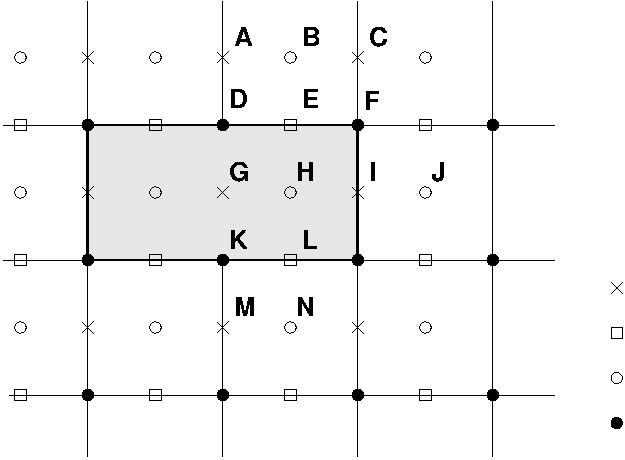
\includegraphics{pics/mask2}%
\end{picture}%
\begin{picture}(348,263)(92,465)
\put(490,552){\makebox(0,0)[lb]{-- $u$ points}}
\put(490,528){\makebox(0,0)[lb]{-- $v$ points}}
\put(490,504){\makebox(0,0)[lb]{-- $\rho$ points}}
\put(490,480){\makebox(0,0)[lb]{-- $\psi$ points}}
\end{picture}
\caption{Masked region within the domain}
\label{fmask1}
\end{figure}

\subsubsection{Velocity}
At the end of every time step, the values of many variables within the
masked region are set to zero by multiplying by the mask for either the
$u$, $v$ or $\rho$ points.  This is appropriate for the $v$ points {\bf
E} and {\bf L} in Fig.\ \ref{fmask1}, since the flow in and out of the
land should be zero.  It is likewise appropriate for the $u$ point at
{\bf I}, but is not necessarily correct for point {\bf G}.  The only
term in the $u$ equation that requires the $u$ value at point {\bf G}
is the horizontal viscosity, which has a term of the form
$\frac{\partial}{\partial \eta} \nu \frac{\partial u}{\partial \eta}$.
Since point {\bf G} is used in this term by both points {\bf A} and
{\bf M}, it is not sufficient to replace its value with that of the
image point for {\bf A}.  Instead, the term $\frac{\partial u}{\partial
\eta}$ is computed and the values at points {\bf D} and {\bf K} are
replaced with the values appropriate for either free-slip or no-slip
boundary conditions.  Likewise, the term $\frac{\partial}{\partial \xi}
\nu \frac{\partial v}{\partial \xi}$ in the $v$ equation must be corrected
at the mask boundaries.

This is accomplished by having a fourth mask array defined at the $\psi$
points, in which the values are set to be no-slip in \code{metrics}.
For no-slip boundaries, we count on the values inside
the land (point {\bf G}) having been zeroed out.  For point {\bf D}, the
image point at {\bf G} should contain minus the value of $u$ at point
{\bf A}.  The desired value of $\frac{\partial u}{\partial \eta}$ is
therefore $2 u_{\bf A}$ while instead we have simply $u_{\bf A}$.
In order to achieve the correct result, we multiply by a mask which
contains the value 2 at point {\bf D}.  It also contains a 2 at point
{\bf K} so that $\frac{\partial u}{\partial \eta}$ there will acquire
the desired value of $-2 u_{\bf M}$. The corner point {\bf F} is set to
have a value of 1.

\subsubsection{Temperature, salinity and surface elevation}

The handling of masks by the temperature, salinity and surface
elevation equations is similar to that in the momentum equations, and
is in fact simpler.  Values of $T$, $S$ and $\zeta$ inside the land
masks, such as point {\bf H} in Fig.\ \ref{fmask1}, are set to zero
after every time step.  This point would be used by the horizontal
diffusion term for points {\bf B}, {\bf J}, and {\bf N}.  This is
corrected by setting the first derivative terms at points {\bf E}, {\bf
I}, and {\bf L} to zero, to be consistent with a no-flux boundary
condition.
Note that the equation of state must be able to handle $T = S = 0$
since this is the value inside masked regions.

%\subsubsection{Free surface and pressure gradients}

%The surface elevation inside the land mask is simply used for setting
%the total depth and therefore the location of the $s$-coordinate
%surfaces.

\subsubsection{Wetting and drying}

There is now an option to have wetting and drying in the model, in
which a cell can switch between being wet or being dry as the tides
come in and go out, for instance. Cells which are masked out as in
Fig.~\ref{fmask1} are never allowed to be wet, however.
\begin{itemize}
   \item In the case of wetting and drying, a critical depth, $D_{crit}$,
is supplied by the user.
   \item The total water depth ($D=h+\zeta$) is compared to $D_{crit}$.
If the water level is less than this depth, no flux is allowed out
of that cell. Water can always flow in and resubmerge the cell.
  \item The wetting and drying only happens during the 2-D
computations; the 3-D computations see a depth of
$D_{crit}$ in the ``dry'' areas.
  \item The ice component now checks for dry cells when computing
the ice rheology.
\end{itemize}

\subsection{Time-stepping overview}

While time stepping the model, we have a stored history of the model fields
at time $n-1$, an estimate of the fields at the current time $n$, and
we need to come up with an estimate for time $n+1$. For reasons of
efficiency, we choose to use a split-explicit time step, integrating
the depth-integrated equations with a shorter time step than the full
3-D equations. There is an integer ratio $M$ between the time steps. The
exact details of how the time stepping is done vary from one version
of ROMS to the next, with the east coast ROMS described here being older
than other branches. Still, all versions have these steps:

\begin{enumerate}
  \item Take a predictor step for at least the 3-D tracers to time
  $n+\frac{1}{2}$.
  \item Compute $\overline{\rho}$ and
$\rho^*$ for use in the depth-integrated time steps, from the density
either at time $n$ or time $n+\frac{1}{2}$.
  \item Depth integrate the 3-D momentum right-hand side terms at
time $n+\frac{1}{2}$ for use in the depth-integrated time steps (or extrapolate
to obtain an estimate of those terms).
  \item Take all the depth-integrated steps. Store weighted
time-means of the $\overline{u}$, $\overline{v}$ fields centered at both
time $n+\frac{1}{2}$ and time $n+1$ (plus $\zeta$ at time $n+1$). The latter
requires this time stepping to extend past time $n+1$, using $M^*$ steps
rather than just $M$.
  \item Use the weighted time-means from depth-integrated fields to
complete the corrector step for the 3-D fields to time $n+1$.
\end{enumerate}
Great care is taken to avoid the introduction of a mode-splitting
instability due to the use of shorter time steps for the depth-integrated
computations.

The mode coupling has evolved through the various ROMS versions,
as shown in Fig.~\ref{ftimestep1} (from \cite{SS2008a}). The time stepping
schemes are also listed in Table~\ref{ttimestep1} and described in
detail in \cite{SS2005} and \cite{SS2008b}; the relevant ones
are described in Appendix~\ref{Frog}.

\begin{figure}[p]
\setlength{\unitlength}{1.0in}%
%
\begin{picture}(6.5,7.5)(0,0)
  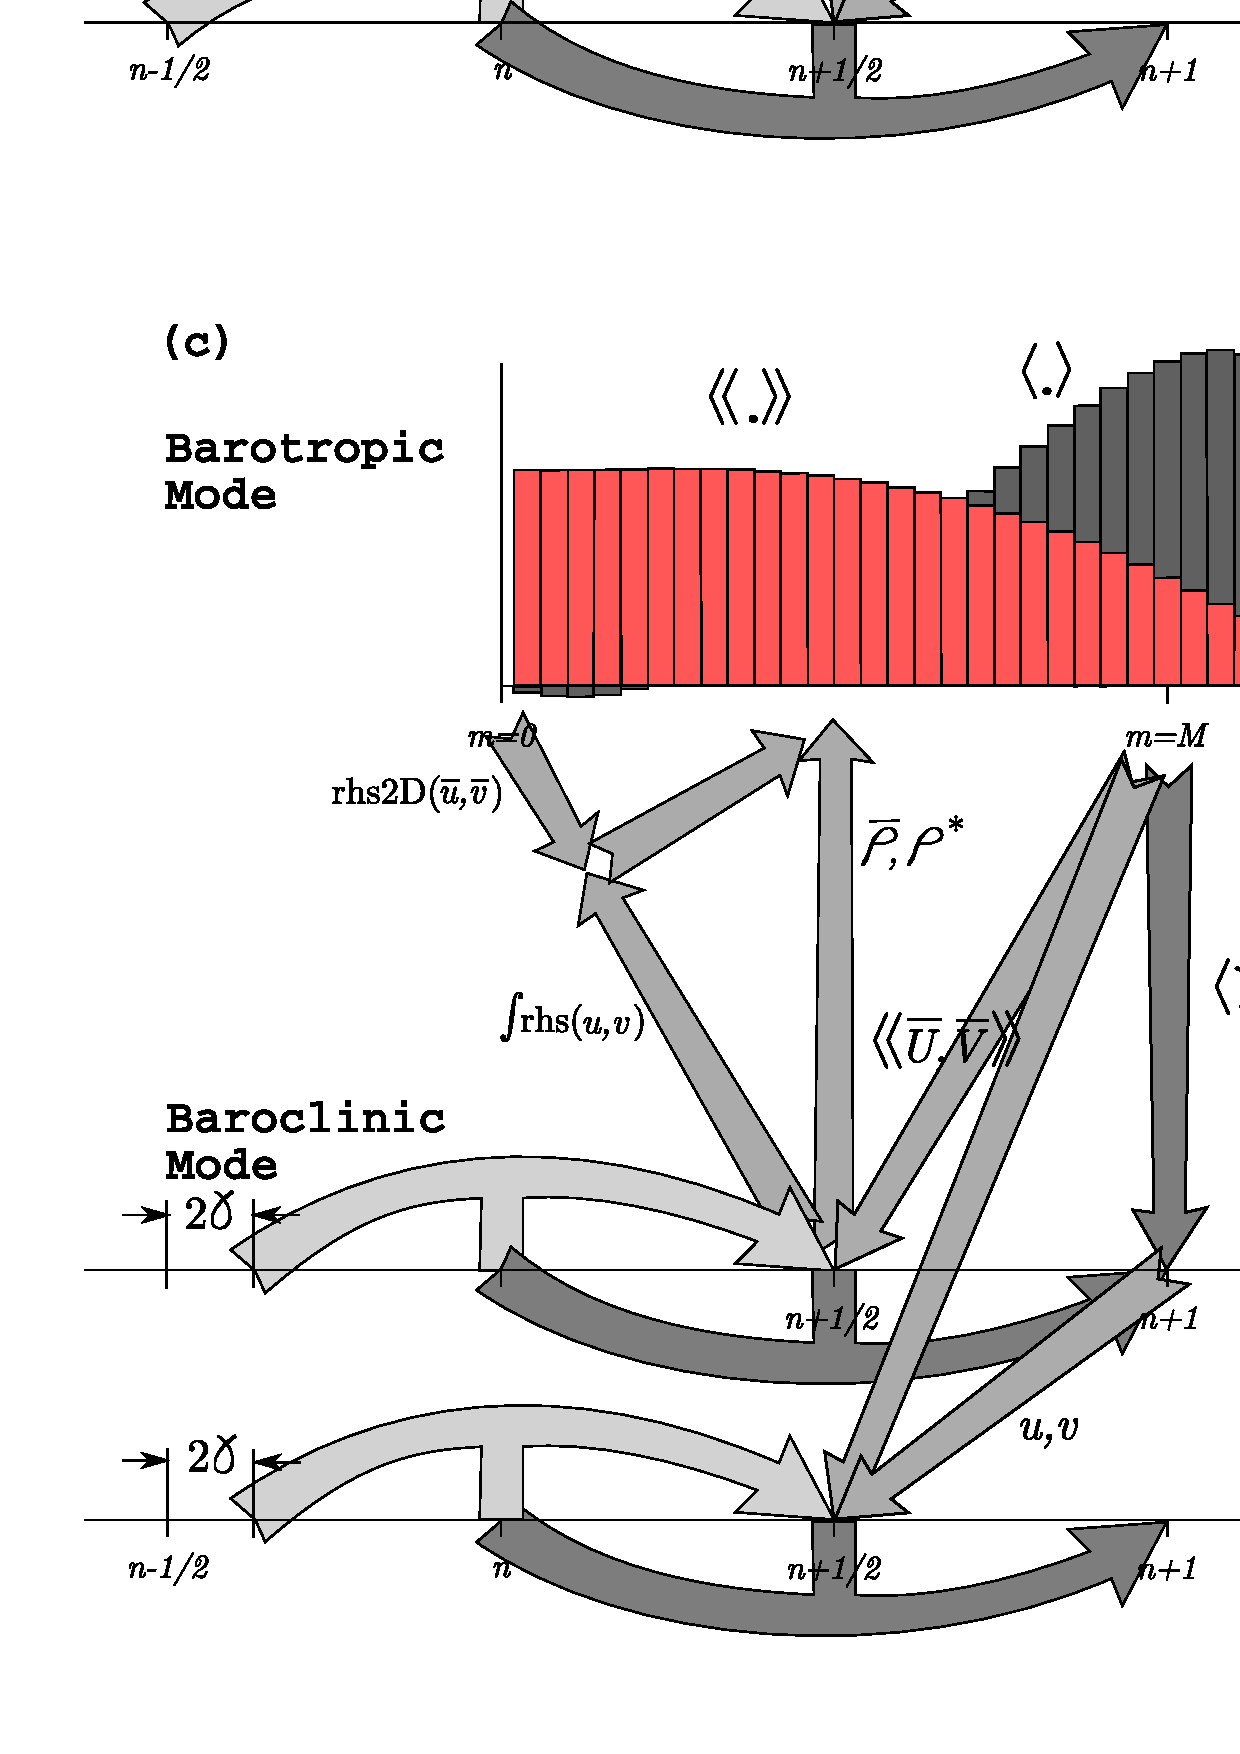
\includegraphics[width=6.5in]{pics/timestep_all}%
\end{picture}%
\caption{Diagrams of the time stepping and mode coupling used in
various ROMS versions. (a) Rutgers University ROMS (from
myroms.org), (b) ROMS AGRIF, (c) UCLA ROMS, described in \cite{SS2005},
(d) non-hydrostatic ROMS (\cite{Kanarska2007}). In all, the curved
arrows update the 3-D fields; those with ``pillars'' are leapfrog
in nature with the pillar representing the r.h.s. terms. Straight
arrows indicate exchange between the barotropic and baroclinic
modes. The shape functions for the fast time steps show just one
option out of many possibilities. The grey function has weights to
produce an estimate at time $n+1$, while the light red function has
weights to produce an estimate at time $n+\frac{1}{2}$.}
 \label{ftimestep1}
\end{figure}

\begin{table}[thb]
 \centerline{
\begin{tabular}{|l|c|c|c|c|c|} \hline
  & SCRUM 3.0 & Rutgers & AGRIF & UCLA & Non-hydrostatic \\
  \hline
  Reference & \cite{Hedstrom2000} & \cite{DAMEE_1} &
  \cite{Penven2006} & \cite{SS2005} & \cite{Kanarska2007} \\
  \hline
  Barotropic  & LF-TR & LF-AM3 with
  & LF-AM3 with & Gen. FB & Gen. FB \\
  mode & & FB feedback & FB feedback\footnote{The generalized FB
  barotropic mode was ported into the newest AGRIF code at the end
  of 2007.} & (AB3-AM4) & (AB3-AM4) \\
  \hline
  2-D $\alpha_{\max}$, iter. & $\sqrt{2}$,
  (2)\footnote{The number in parentheses (e.g., 2) indicates the
  number of r.h.s. computations per time step. If there are two
  parenthesized number, the first one is for momenta, the second for
  tracers.} & 1.85, (2) & 1.85,
  (2) & 1.78, (1) & 1.78, (1) \\
  \hline
  3-D momenta & AB3 & AB3 & LF-AM3 & LF-AM3 & AB3 (mod) \\
  \hline
  Tracers & AB3 & LF-TR & LF-AM3 & LF-AM3 & AB3 (mod) \\
  \hline
  Internal & AB3 & Gen.\ FB &
  LF-AM3, & LF-AM3, &
  Gen.\ FB \\
  waves & & (AB3-TR) & FB feedback & FB feedback & (AB3-AM4) \\
  \hline
  $\alpha_{\max}$, advect. & 0.72 & 0.72 & 1.587 &
  1.587 & 0.78 \\
  \hline
  $\alpha_{\max}$, Cor. & 0.72 & 0.72 & 1.587 &
  1.587 & 0.78 \\
  \hline
  $\alpha_{\max}$, int. w. & 0.72, (1) & 1.14,
  (1,2) & 1.85, (2) &
  1.85, (2) & 1.78, (1) \\
  \hline
  \end{tabular}
  }
\label{ttimestep1}
\caption{The time stepping schemes used in the various ROMS versions.
$\alpha \equiv \omega \delta t$ is the Courant number and $\omega=ck$
is the frequency for a wave component with wavenumber $k$.}
\end{table}

\subsection{Conservation properties}
\label{Enrg}
From Shchepetkin and McWilliams (2005) \cite{SS2005}, we have a
tracer concentration equation in advective form:
\begin{equation}
  \frac{\partial C}{\partial t} + (u \cdot \nabla) C = 0
  \label{eqt1}
\end{equation}
and also a tracer concentration equation in conservation form:
\begin{equation}
   \frac{\partial C}{\partial t} + \nabla \cdot (u C) = 0.
  \label{eqt2}
\end{equation}
The continuity equation:
\begin{equation}
   ( \nabla \cdot u) = 0
\end{equation}
can be used to get from one tracer equation to the other.
As a consequence of eq.~(\ref{eqt1}), if the tracer is spatially
uniform, it will remain so regardless of the velocity field
(constancy preservation). On the other hand, as a consequence of
(\ref{eqt2}), the volume integral of the tracer concentration is conserved
in the absence of internal sources and fluxes through the boundary. Both
properties are valuable and should be retained when constructing numerical
ocean models.

The semi-discrete form of the tracer equation
(\ref{st15}) is:
\begin{equation}
   \frac{\partial}{\partial t} \left( \frac{H_z C}{m n} \right)
   + \delta_{\xi} \left(
   \frac{u \overline{H_z}^\xi \overline{C}^\xi }{\overline{n}^\xi} \right)
   + \delta_{\eta} \left(
   \frac{v \overline{H_z}^\eta \overline{C}^\eta }{\overline{m}^\eta} \right)
   + \delta_\sigma \left( \overline{C}^\sigma
   \frac{H_z \Omega}{m n} \right) =
\\ \vspace{2mm}
   \frac{ 1}{mn} \frac{\partial}{\partial \sigma}
   \left( \frac{K_m}{\Delta z} \frac{\partial C}{\partial \sigma} \right) +
   {\cal D}_C + {\cal F}_C
\label{tfull}
\end{equation}
Here $\delta_{\xi}$, $\delta_{\eta}$ and $\delta_\sigma$ denote simple
centered finite-difference approximations to $\partial / \partial \xi$,
$\partial / \partial \eta$ and $\partial / \partial \sigma$ with the
differences taken over the distances $\Delta\xi$, $\Delta\eta$ and
$\Delta \sigma$, respectively. $\Delta z$ is the vertical distance from one
$\rho$ point to another. $\overline{ ( \hspace{5mm} )}^{\xi}$,
$\overline{ ( \hspace{5mm} )}^{\eta}$ and $\overline{ ( \hspace{5mm}
)}^\sigma$ represent averages taken over the distances $\Delta\xi$, $\Delta
\eta$ and $\Delta \sigma$. % $I_\sigma^0$ indicates a second-order vertical
%integral computed as a sum from level $\sigma$ to the surface at
%$\sigma=0$.

The finite volume version of the same equation is no different,
except that a quantity $C$ is defined as the volume-averaged
concentration over the grid box $\Delta V$:
\begin{equation}
   C = \frac{mn}{H_z} \int_{\Delta V} \frac{H_z C}{mn} \delta \xi
   \, \delta \eta \, \delta \sigma
\end{equation}
The quantity  $\left(
\frac{u \overline{H_z}^\xi \overline{C}^\xi}{\overline{n}^\xi} \right)$
is the flux through an interface between adjacent grid boxes.

This method of averaging was chosen because it internally conserves
first moments in the model domain, although it is still possible to
exchange mass and energy through the open boundaries. The method is
similar to that used in Arakawa and Lamb \cite{AL}; though their
scheme also conserves enstrophy. Instead, we will focus on (nearly) retaining
constancy preservation while coupling the barotropic
(depth-integrated) equations and the baroclinic equations.

The time step in eq.~(\ref{tfull}) is assumed to be from time $n$ to
time $n+1$, with the other terms being evaluated at time
$n+\frac{1}{2}$ for second-order accuracy.
Setting $C$ to 1 everywhere reduces eq.~(\ref{tfull}) to:
\begin{equation}
   \frac{\partial}{\partial t} \left( \frac{H_z}{m n} \right)
   + \delta_{\xi} \left(
   \frac{u \overline{H_z}^\xi }{\overline{n}^\xi} \right)
   + \delta_{\eta} \left(
   \frac{v \overline{H_z}^\eta}{\overline{m}^\eta} \right)
   + \delta_\sigma \left( 
   \frac{H_z \Omega}{m n} \right) = 0
\label{contfull}
\end{equation}
If this equation holds true for the step from time $n$ to time $n+1$, then
our constancy preservation will hold.

In a hydrostatic model such as ROMS, the discrete continuity
equation is needed to compute vertical velocity rather than grid-box
volume $\frac{H_z}{m n}$ (the latter is controlled by changes in
$\zeta$ in the barotropic mode computations). Here, $\frac{H_z
\Omega}{m n}$ is the finite-volume flux across the {\em moving}
grid-box interface, vertically on the $w$ grid.

The vertical integral of the continuity eq.~(\ref{st17}), using
the vertical boundary conditions on $\Omega$, is:
\begin{equation}
   \frac{\partial}{\partial t} \left( \frac{\zeta}{mn} \right) +
   \delta_{\xi} \left(
   \frac{\overline{u} \overline{D}^\xi }{\overline{n}^\xi} \right)
   + \delta_{\eta} \left(
   \frac{\overline{v} \overline{D}^\eta}{\overline{m}^\eta} \right)
   = 0
\label{zeta1}
\end{equation}
where $\zeta$ is the surface elevation, $D= h+\zeta$ is the total
depth, and $\overline{u},\overline{v}$ are the depth-integrated
horizontal velocities. This equation and the corresponding 2-D
momentum equations are time stepped on a shorter time step than 
eq.~(\ref{tfull}) and the other 3-D equations. Due to the details in
the mode coupling, it is only possible to maintain constancy
preservation to the accuracy of the barotropic time steps.

\subsection{Depth-integrated equations}
\label{Vort}
The depth average of a quantity $A$ is given by:
\begin{equation}
   \overline{A} = \frac{1}{D} \int_{-1}^0 H_z A d\sigma
\end{equation}
where the overbar indicates a vertically averaged quantity and
\begin{equation}
   D \equiv \zeta(\xi, \eta, t) + h(\xi, \eta)
\end{equation}
is the total depth of the water column.  The vertical integral of
equation (\ref{st13}) is:
%{\samepage
\begin{multline}
   \frac{\partial}{\partial t} \left( \frac{D \overline{u}}{mn} \right)
   + \frac 
   {\partial}{\partial \xi} \left( \frac{D \overline{uu}}{n} \right )
   + \frac 
   {\partial}{\partial \eta} \left( \frac{D \overline{uv}}{m} \right)
   - \frac{Df\overline{v}}{mn}
\\ \vspace{1mm}
   - \left[ \overline{vv}
   \frac{\partial}{\partial \xi}
   \left( \frac{1}{n} \right) - \overline{uv}
   \frac{\partial}{\partial \eta} \left(
   \frac{1}{m} \right) \right] D = 
   - \frac{D}{n}
   \left( \frac{\partial \overline{\phi_2}}{\partial \xi} +
   g \frac{\partial \zeta}{\partial \xi} \right)
\\ \vspace{1mm}
   + \frac{ D}{mn}
   \left( \overline{\cal F}_u + \overline{\cal D}_{h_u} \right) 
   + \frac{1}{mn} \left( \tau^{\xi}_s - \tau^{\xi}_b \right)
\label{ubar1}
\end{multline}
%}
where $\phi_2$ includes the $\frac{\partial z}{\partial \xi}$ term,
$\overline{\cal D}_{h_u}$ is the horizontal viscosity, and the
vertical viscosity only contributes through the upper and lower
boundary conditions.  The corresponding vertical integral of equation
(\ref{st14}) is:
%{\samepage
\begin{multline}
   \frac{\partial}{\partial t} \left( \frac{D \overline{v}}{mn} \right)
   + \frac 
   {\partial}{\partial \xi} \left( \frac{D \overline{uv}}{n} \right )
   + \frac 
   {\partial}{\partial \eta} \left( \frac{D \overline{vv}}{m} \right)
   + \frac{Df\overline{u}}{mn}
\\ \vspace{1mm}
   + \left[ \overline{uv}
   \frac{\partial}{\partial \xi}
   \left( \frac{1}{n} \right) - \overline{uu}
   \frac{\partial}{\partial \eta} \left(
   \frac{1}{m} \right) \right] D = 
   - \frac{D}{m}
   \left( \frac{\partial \overline{\phi_2}}{\partial \eta} +
   g \frac{\partial \zeta}{\partial \eta} \right)
\\ \vspace{1mm}
   + \frac{ D}{mn}
   \left( \overline{\cal F}_v + \overline{\cal D}_{h_v} \right) 
   + \frac{1}{mn} \left( \tau^{\eta}_s - \tau^{\eta}_b \right) .
\label{vbar1}
\end{multline}
%}
We also need the vertical integral of equation (\ref{st17}), shown
above as eq.~ (\ref{zeta1}).

The presence of a free surface introduces waves which propagate at a
speed of $\sqrt{gh}$.  These waves usually impose a more severe
time-step limit than any of the internal processes.  We have therefore
chosen to solve the full equations by means of a split time step.  In
other words, the depth integrated equations (\ref{ubar1}),
(\ref{vbar1}), and (\ref{zeta1}) are integrated using a short time step
and the values of $\overline{u}$ and $\overline{v}$ are used
to replace those found by integrating the full equations on a longer
time step.  A diagram of the barotropic time stepping is shown in
Fig.~\ref{ftspl}.
\begin{figure}[htb]
\setlength{\unitlength}{1.00in}%
%
\begin{picture}(5,2)(0,0.3)%
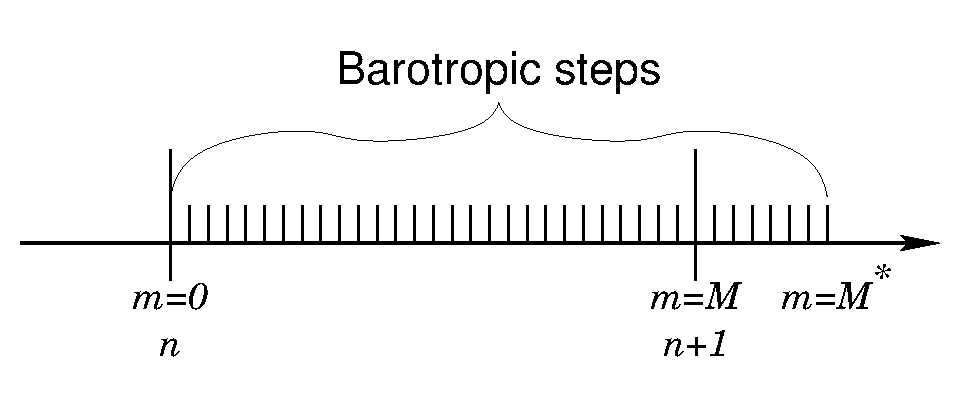
\includegraphics{pics/shortstep}%
\end{picture}%
 
 \caption{The split time stepping used in the model.}
 \label{ftspl}
\end{figure}

Some of the terms in equations (\ref{ubar1}) and (\ref{vbar1}) are
updated on the short time step while others are not.  The contributions
from the slow terms are computed once per long time step and stored.  If
we call these terms $R_{u_{\rm slow}}$ and $R_{v_{\rm slow}}$, equations
(\ref{ubar1}) and (\ref{vbar1}) become:
%{\samepage
\begin{multline}
   \frac{\partial}{\partial t} \left( \frac{D \overline{u}}{mn} \right)
   + \frac{\partial}{\partial \xi}
   \left( \frac{D \overline{u}\,\overline{u}}{n} \right)
   + \frac{\partial}{\partial \eta}
   \left( \frac{D \overline{u}\,\overline{v}}{m} \right)
   - \frac{Df\overline{v}}{mn}
\\ \vspace{1mm}
   - \left[ \overline{v}\,\overline{v}
   \frac{\partial}{\partial \xi}
   \left( \frac{1}{n} \right) - \overline{u}\,\overline{v}
   \frac{\partial}{\partial \eta} \left(
   \frac{1}{m} \right) \right] D = R_{u_{\rm slow}} -
   \frac{gD}{n} \frac{\partial \zeta}{\partial \xi}
    + \frac{D}{mn} {\cal D}_{\overline{u}}
   - \frac{1}{mn} \tau^{\xi}_b
\label{ubar2}
\end{multline}
%}  
%{\samepage
\begin{multline}
   \frac{\partial}{\partial t} \left( \frac{D \overline{v}}{mn} \right)
   + \frac{\partial}{\partial \xi}
   \left( \frac{D \overline{u}\,\overline{v}}{n} \right)
   + \frac{\partial}{\partial \eta}
   \left( \frac{D \overline{v}\,\overline{v}}{m} \right)
   + \frac{Df\overline{u}}{mn}
\\ \vspace{1mm}
   + \left[ \overline{u}\,\overline{v}
   \frac{\partial}{\partial \xi}
   \left( \frac{1}{n} \right) - \overline{u}\,\overline{u}
   \frac{\partial}{\partial \eta} \left(
   \frac{1}{m} \right) \right] D = R_{v_{\rm slow}} -
   \frac{gD}{m} \frac{\partial \zeta}{\partial \eta}
    + \frac{ D}{mn} {\cal D}_{\overline{v}}
   - \frac{1}{mn} \tau^{\eta}_b .
\label{vbar2}
\end{multline}
%}
When time stepping the model, we compute the right-hand-sides for
equations (\ref{st13}) and (\ref{st14}) as well as the
right-hand-sides for equations (\ref{ubar2}) and (\ref{vbar2}).  The
vertical integral of the 3-D right-hand-sides are obtained and then the
2-D right-hand-sides are subtracted.  The resulting fields are the slow
forcings $R_{u_{\rm slow}}$ and $R_{v_{\rm slow}}$.  This was found to
be the easiest way to retain the baroclinic contributions of the
non-linear terms such as $\overline{uu} - \overline{u}\,\overline{u}$.

The model is time stepped from time $n$ to time $n+1$ by using short
time steps on equations (\ref{ubar2}), (\ref{vbar2}) and (\ref{zeta1}).
Equation (\ref{zeta1}) is time stepped first, so that an estimate of the
new $D$ is available for the time rate of change terms
in equations (\ref{ubar2}) and (\ref{vbar2}).
A third-order predictor-corrector time stepping is used.
In practice, we actually time step all the way to time
$(n+\code{dtfast} \times M^\star)$,
while maintaining weighted averages of the values of $\overline{u}$,
$\overline{v}$ and $\zeta$.  The averages are used to replace the
values at time $n+1$ in both the baroclinic and barotropic modes,
and for recomputing the vertical grid spacing $H_z$.
Fig.~\ref{fbarostep1} shows one option for how these weights might look.

\begin{figure}[tbp]
\setlength{\unitlength}{1.in}%
\begin{picture}(6.5,6.5)(0,0)
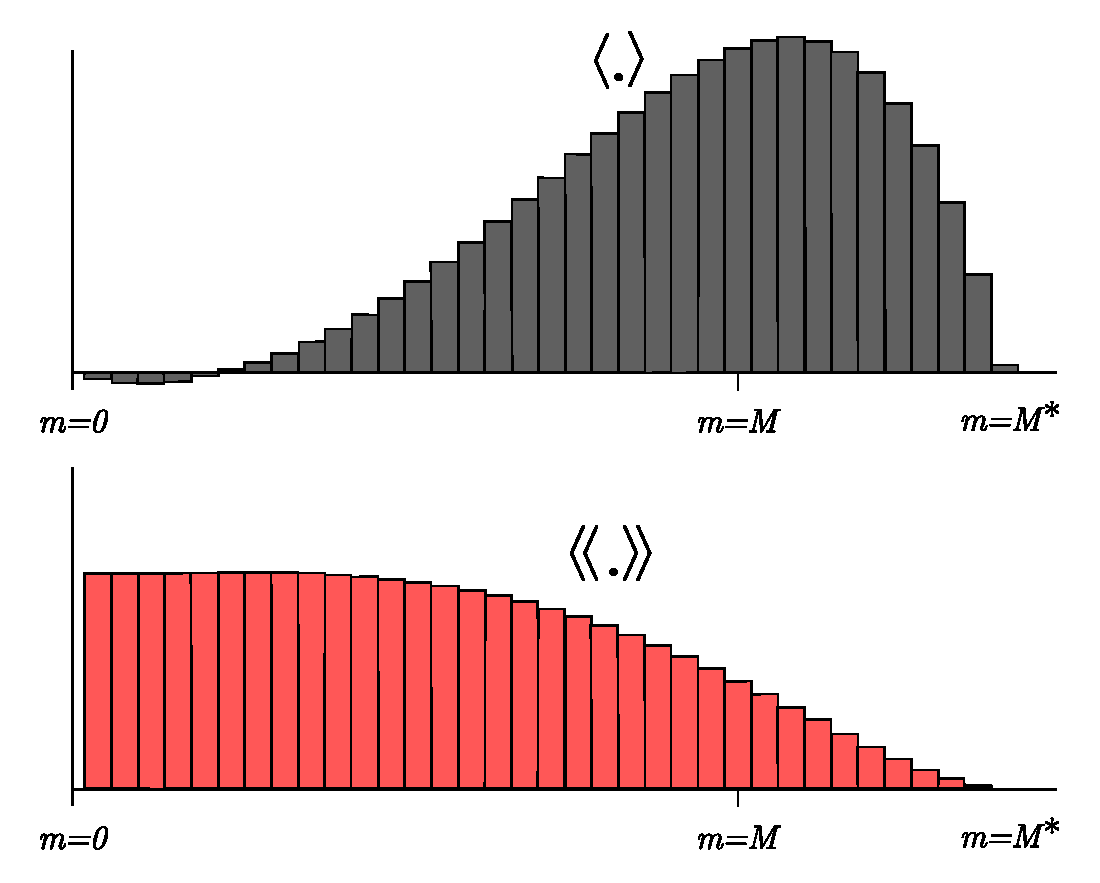
\includegraphics[width=6.5in]{pics/barostep}%
\end{picture}%
\caption{Weights for the barotropic time stepping. The upper panel
shows the primary weights, centered at time $n+1$, while the lower panel shows
the secondary weights weights, centered at time $n+\frac{1}{2}$.}
\label{fbarostep1}
\end{figure}

The primary weights, $a_m$, are used to compute $\langle \zeta
\rangle^{n+1} \equiv \sum_{m=1}^{M^\star} a_m \zeta^m$. There is a
related set of secondary weights $b_m$, used as $\langle \! \langle
\overline{u} \rangle \! \rangle^{n+\frac{1}{2}} \equiv \sum_{m=1}^{M^\star} b_m
\overline{u}^m$. In order to maintain constancy preservation, this
relation must hold:
\begin{equation}
  \langle \zeta \rangle_{i,j}^{n+1} = \langle \zeta \rangle_{i,j}^n -
  (mn)_{i,j} \Delta t \left[ \left\langle \!\! \left\langle
  \frac{D\overline u}{n} \right\rangle \!\!
  \right\rangle_{i+\frac{1}{2},j}^{n+\frac{1}{2}}
  - \left\langle \!\! \left\langle \frac{D\overline u}{n} \right\rangle
  \!\! \right\rangle_{i-\frac{1}{2},j}^{n+\frac{1}{2}} +
  \left\langle \!\! \left\langle
  \frac{D\overline v}{m} \right\rangle \!\!
  \right\rangle_{i,j+\frac{1}{2}}^{n+\frac{1}{2}}
  - \left\langle \!\! \left\langle \frac{D\overline v}{m} \right\rangle
  \!\! \right\rangle_{i,j-\frac{1}{2}}^{n+\frac{1}{2}} \right]
\label{zeta3}
\end{equation}
Shchepetkin and McWilliams (\cite{SS2005}) introduce a range of
possible weights, but the ones used here have a shape function:
\begin{equation}
   A(\tau) = A_0 \left\{ \left( \frac{\tau}{\tau_0} \right)^p \left[ 1-
   \left(\frac{\tau}{\tau_0} \right)^q \right] - r \frac{\tau}{\tau_0}
   \right\}
\label{weights}
\end{equation}
where $p, q$ are parameters and $A_0, \tau_0$, and $r$ are chosen to
satisfy normalization, consistency, and second-order accuracy
conditions,
\begin{equation}
   I_n = \int_0^{\tau^\star} \tau^n A(\tau) d \tau = 1, \quad n=0,1,2
\label{second}
\end{equation}
using Newton iterations. $\tau^\star$ is the upper limit of $\tau$
with $A(\tau) \geq 0$. In practice we initially set
$$
  A_0 = 1, r = 0 \mbox{and} \tau = \frac{(p+2)(p+q+2)}{(p+1)(p+q+1)}
$$
compute $A(\tau)$ using eq.~(\ref{weights}), normalize using:
\begin{equation}
   \sum_{m=1}^{M^\star} a_m \equiv 1, \quad
   \sum_{m=1}^{M^\star} a_m\frac{m}{M} \equiv 1,
\end{equation}
and adjust $r$ iteratively to satisfy the $n=2$ condition of
(\ref{second}). We are using values of $p=2$, $q=4$, and $r=0.284$.
This form allows some negative weights for small $m$, allowing
$M^\star$ to be less than $1.5M$.

ROMS also supports an older cosine weighting option, which isn't
recommended since it is only first-order accurate.

\subsection{Density in the mode coupling}

Equation (\ref{ubar2}) contains the term $R_{u_{\rm slow}}$,
computed as the difference between the 3-D right-hand-side and the
2-D right-hand-side. The pressure gradient therefore has the form:
\begin{equation}
   -\frac{g D}{n} \frac{\partial \zeta}{\partial \xi} +
   \left[\frac{g D}{n} \frac{\partial \zeta}{\partial \xi} + {\cal F}
   \right]
\end{equation}
where the term in square brackets is the mode coupling term and is
held fixed over all the barotropic steps and
\begin{equation}
  {\cal F} = - \frac{1}{\rho_0 n} \int_{-h}^\zeta \frac{\partial
  P}{\partial \xi} dz
\end{equation}
is the vertically integrated pressure gradient. The latter is a function
of the bathymetry, free surface gradient, and the free surface itself,
as well as the vertical distribution of density.

The disadvantage of this approach is that after the barotropic time
stepping is complete and the new free surface is substituted into
the full baroclinic pressure gradient, its vertical integral will
no longer be equal to the sum of the new surface slope term and the
original coupling term based on the old free surface. This is one
form of mode-splitting error which can lead to trouble because the
vertically integrated pressure gradient is not in balance with the
barotropic mass flux.

Instead, let us define the following:
\begin{equation}
  \overline{\rho} = \frac{1}{D} \int_{-h}^\zeta \rho dz , \quad
  \rho^\star = \frac{1}{\frac{1}{2} D^2} \int_{-h}^\zeta
  \left\{ \int_z^\zeta \rho dz^{\prime} \right\} dz
\end{equation}
Changing the vertical coordinate to $\sigma$ yields:
\begin{equation}
  \overline{\rho} =  \int_{-1}^0 \rho d\sigma , \quad
  \rho^\star = 2 \int_{-1}^0
  \left\{ \int_\sigma^0 \rho d\sigma^{\prime} \right\} d\sigma
\end{equation}
which implies that $\overline{\rho}$ and $\rho^\star$ are actually
independent of $\zeta$ as long as the density profile $\rho =
\rho(\sigma)$ does not change. The vertically integrated pressure
gradient becomes:
\begin{equation}
   -\frac{1}{\rho_0} \frac{g}{n} \left\{ \frac{\partial}{\partial \xi}
   \left( \frac{\rho^\star D^2}{2} \right) - \overline{\rho} D
   \frac{\partial h}{\partial \xi} \right\} = -\frac{1}{\rho_0}
   \frac{g}{n} D \left\{ \rho^\star \frac{\partial \zeta}{\partial \xi} +
   \frac{D}{2} \frac{\partial \rho^\star}{\partial \xi} + (\rho^\star -
   \overline{\rho}) \frac{\partial h}{\partial \xi} \right\}
\end{equation}
In the case of uniform density $\rho_0$, we obtain $\rho^\star \equiv
\overline{\rho} \equiv \rho_0$, but we otherwise have two new terms.
The accuracy of these terms depends on an accurate vertical
integration of the density, as described in Shchepetkin and
McWilliams (2005, \cite{SS2005}).

\subsection{Time stepping: internal velocity modes and tracers}
The momentum equations (\ref{st13}) and(\ref{st14}) are advanced before
the tracer equation, by computing all the terms except the vertical
viscosity and then using the implicit scheme described in \S\ref{Vfric}
to find the new values for $u$ and $v$. The depth-averaged component
is then removed and replaced by the $\langle \overline{u} \rangle$
and $\langle \overline{v} \rangle$ computed as in \S\ref{Vort}.
A third-order Adams-Bashforth (AB3) time stepping is used, requiring
multiple right-hand-side time levels (see Appendix~\ref{Frog}). These
stored up r.h.s. values can be used to extrapolate to a value at
time $n+\frac{1}{2}$ for use in the barotropic steps as shown in
Fig.~\ref{ftimestep1}.

The tracer concentration equation (\ref{tfull}) is advanced in a
predictor-corrector leapfrog-trapezoidal step, with great care taken to
optimize both the conservation and constancy-preserving properties of the
continuous equations. The corrector step can maintain both, as long as it
uses velocities and column depths which satisfy eq.~(\ref{zeta3}). This
also requires tracer values centered at time $n+\frac{1}{2}$, obtained
from the predictor step. The vertical diffusion is computed as in
\S\ref{Vfric}.

The predictor step cannot be both constancy-preserving and conservative; it
was therefore decided to make it constancy-preserving. Also, since it is
only being used to compute the advection for the corrector step, the
expensive diffusion operations are not carried out during the predictor step.

The preceeding notes on tracer advection refer to all but the MPDATA
option. The MPDATA algorithm has its own predictor-corrector with
emphasis on not allowing values to exceed their original range;
it therefore gives up the constancy-preservation. This is most
noticeable in shallow areas with large tides.

\subsection{Advection schemes}
\label{Advect}
Thus far, the advection scheme presented here is a centered
second-order scheme. This scheme is known to have some unfortunate
properties in the presence of strong gradients, such as large over- and
under-shoots of tracers, leading to the need for large amounts of
horizontal smoothing. SCRUM also provides two alternative advection
schemes with better behavior in many situations. At present, the
alternatives are only implemented in the full 3-D engine of the model.

\subsubsection{Third-order Upwind}
There is a class of third-order upwind advection schemes, both
one-dimensional (Leonard \cite{Leonard79}) and two-dimensional (Rasch
\cite{Rasch94}). This scheme is known as UTOPIA (Uniformly Third-Order
Polynomial Interpolation Algorithm). Applying flux limiters to UTOPIA
is explored in Thuburn \cite{Thuburn96}, although it is not implemented
in SCRUM. The two-dimensional formulation in Rasch contains terms of
order $u^2\psi$ and $u^3\psi$, including cross terms ($uv\psi$). The
terms which are nonlinear in velocity have been dropped in SCRUM,
leaving one extra upwind term in the computation of the advective
fluxes:
\begin{align}
   F^\xi &= \frac{H_z u}{n} \left( \psi - \gamma \frac{\partial^2
   \psi}{\partial \xi^2} \right) \\
   F^\eta &= \frac{H_z v}{m} \left( \psi - \gamma \frac{\partial^2
   \psi}{\partial \eta^2} \right)
\end{align}
The second derivative terms are centered on a $\rho$ point in the grid,
but are needed at a $u$ or $v$ point in the flux. The upstream value is
used [see equation (\ref{equp})]. The value of $\gamma$ in the model is
$\frac{1}{8}$ while that in Rasch \cite{Rasch94} is $\frac{1}{6}$.

Because the third-order upwind scheme is designed to be
two-dimensional, it is not used in the vertical (though one might argue
that we are simply performing one-dimensional operations here).
Instead, we use a centered fourth-order scheme in the vertical when
the third-order upwind option is turned on:
\begin{equation}
   F^s = \frac{H_z w}{mn} \left[
     - \frac{1}{16} \psi_{i,j,k-1} + \frac{9}{16} \psi_{i,j,k} +
       \frac{9}{16} \psi_{i,j,k+1} - \frac{1}{16} \psi_{i,j,k+2} \right]
\end{equation}

One advantage of UTOPIA over MPDATA is that it can be used on
variables having both negative and positive values. Therefore,
it can be used on velocity as well as scalars (is there a reference for
this?). For the $u$-velocity, we have:
\begin{align}
   F^\xi &= \left(u - \gamma \frac{\partial^2 u}{\partial \xi^2} \right)
   \left[ \frac{H_z u}{n} - \gamma \frac{\partial^2}{\partial \xi^2}
   \left( \frac{H_z u}{n} \right) \right] \\
   F^\eta &= \left(u - \gamma \frac{\partial^2 u}{\partial \eta^2}
     \right)
   \left[ \frac{H_z v}{m} - \gamma \frac{\partial^2}{\partial \xi^2}
   \left( \frac{H_z v}{m} \right) \right] \\
   F^\sigma &= \frac{H_z w}{mn} \left[
     - \frac{1}{16} u_{i,j,k-1} + \frac{9}{16} u_{i,j,k} +
       \frac{9}{16} u_{i,j,k+1} - \frac{1}{16} u_{i,j,k+2} \right]
\end{align}
while for the $v$-velocity we have:
\begin{align}
   F^\xi &= \left(v - \gamma \frac{\partial^2 v}{\partial \xi^2} \right)
   \left[ \frac{H_z u}{n} - \gamma \frac{\partial^2}{\partial \eta^2}
   \left( \frac{H_z u}{n} \right) \right] \\
   F^\eta &= \left(v - \gamma \frac{\partial^2 v}{\partial \eta^2}
     \right)
   \left[ \frac{H_z v}{m} - \gamma \frac{\partial^2}{\partial \eta^2}
   \left( \frac{H_z v}{m} \right) \right] \\
   F^\sigma &= \frac{H_z w}{mn} \left[
     - \frac{1}{16} v_{i,j,k-1} + \frac{9}{16} v_{i,j,k} +
       \frac{9}{16} v_{i,j,k+1} - \frac{1}{16} v_{i,j,k+2} \right]
\end{align}
In all these terms, the second derivatives are evaluated at an upstream
location.

\subsection{Determination of the vertical velocity and density fields}
\label{EOS}
Having obtained a complete specification of the $u,v,T,$ and $S$ fields
at the next time level by the methods outlined above, the vertical
velocity and density fields can be calculated.  The vertical velocity
is obtained by combining equations (\ref{st17}) and (\ref{zeta1}) to
obtain:
\begin{equation}
   \frac{\partial}{\partial \xi} \left( \frac{H_z u}{n} \right) +
   \frac{\partial}{\partial \eta} \left( \frac{H_z v}{m} \right) +
   \frac{\partial}{\partial \sigma}\left( \frac{H_z \Omega}{mn} \right)
   - \frac{\partial}{\partial \xi} \left( \frac{D \overline{u}}{n}
   \right) -
   \frac{\partial}{\partial \eta} \left( \frac{D \overline{v}}{m}
   \right)  = 0 .
\label{zeta2}
\end{equation}
Solving for $H_z \Omega / mn$ and using the semi-discrete notation of
\S\ref{Enrg} we obtain:
\begin{equation}
   \frac{H_z \Omega}{mn} =  \int  \left[
   \delta_{\xi} \left( \frac{\overline{u} \overline{D}^{\xi}}
   {\overline{n}^{\xi}} \right) +
   \delta_{\eta} \left( \frac{\overline{v} \overline{D}^{\eta}}
   {\overline{m}^{\eta}} \right) -
   \delta_{\xi} \left( \frac{u \overline{H_z}^{\xi}}
   {\overline{n}^{\xi}} \right) - 
   \delta_{\eta} \left( \frac{v \overline{H_z}^{\eta}}
   {\overline{m}^{\eta}} \right)  \right] d\sigma .
\label{omega}
\end{equation}
The integral is actually computed as a sum from the bottom upwards and
also as a sum from the top downwards.  The value used is a linear
combination of the two, weighted so that the surface down value is used
near the surface while the other is used near the bottom.

The density is obtained from temperature and salinity via an
equation of state.  SCRUM provides a choice of a nonlinear equation
of state $\rho = \rho(T,S,z)$ or a linear equation of state $\rho =
\rho(T)$.  The nonlinear equation of state has been modified and now
corresponds to the UNESCO equation of state as derived by Jackett and
McDougall \cite{Jackett}.  It computes {\sl in situ} density as a
function of potential temperature, salinity and pressure.

Warning: although we have used it quite extensively, McDougall
(personal communication) claims that the single-variable ($\rho =
\rho(T)$) equation of state is not dynamically appropriate as is.
He has worked out the extra source and sink terms required, arising
from vertical motions and the compressibility of water.  They are
quite complicated and we have not implemented them to see if they
alter the flow.

\subsection{The pressure gradient terms}
\label{PG}
The pressure gradient terms in equations (\ref{st13}) and
(\ref{st14}) are written in the form
\begin{equation}
  H_z \nabla \phi + \frac{g \rho H_z}{\rho_o} \nabla z
  + g H_z \nabla \zeta
\label{prgs}
\end{equation}
This is the form traditionally used in sigma-coordinate models to
account for the horizontal differences being taken along surfaces of
constant $\sigma$.  This form can be shown to lead to significant
errors when $|\nabla h|$ is large (Haney \cite{Haney}; and Beckmann
and Haidvogel \cite{BH93}). Shchepetkin....

\subsection{Open boundary conditions}
Need update for ROMS here...

\subsubsection{Gradient boundary condition}
This boundary condition is extremely simple and consists of setting the
gradient of a field to zero at the edge. The outside value is set equal
to the closest interior value. It is probably too simple to be useful
in realistic problems.

\subsubsection{Radiation boundary condition}
In realistic domains, open boundary conditions can be extremely
difficult to get right. There can be situations where incoming flow and
outgoing flow happen along the same boundary or even at the same
horizontal location. Orlanski \cite{Orlanski76} proposed a radiation
scheme in which a local phase velocity is computed and used to radiate
things out (if it is indeed going out). This works well for a wave
propagating normal to the boundary, but has problems when waves
approach the boundary at an angle. Raymond and Kuo \cite{Raymond84}
have modified the scheme to account for propagation in all three
directions. In SCRUM, only the two horizontal directions are accounted
for:
\begin{equation}
   \frac{\partial \psi}{\partial t} = - \left( C_x \frac{\partial
   \psi}{\partial \xi} + C_y \frac{\partial \psi}{\partial \eta}) \right)
\label{eqrk}
\end{equation}
where
\begin{align}
   C_x & = \frac{F \frac{\partial \psi}{\partial \xi}}{
   \left( \frac{\partial \psi}{\partial \xi} \right)^2 +
   \left( \frac{\partial \psi}{\partial \eta} \right)^2 } \\
   C_y & = \frac{F \frac{\partial \psi}{\partial \eta}}{
   \left( \frac{\partial \psi}{\partial \xi} \right)^2 +
   \left( \frac{\partial \psi}{\partial \eta} \right)^2 } \\
   F & = - \frac{\partial \psi}{\partial t}
\end{align}
These terms are evaluated at the closest interior point in a manner
consistent with the time stepping scheme used. The phase velocities are
limited so that the local CFL condition is satisfied. They are then
applied to the boundary point using equation (\ref{eqrk}), again using
a consistent time stepping scheme. Raymond and Kuo give the form used
for centered differencing and a leapfrog time step while SCRUM uses
one-sided differences.

The radiation approach is appropriate for waves leaving the domain. A
check is made to see which way the phase velocity is headed. If it is
entering the domain, a zero gradient condition is applied.

%%%%\section{Support Programs for Initialization}
\label{Progs}

Links to all the programs mentioned here are under the ROMS web site:
\begin{verbatim}
      http://marine.rutgers.edu/po/models/roms.html
\end{verbatim}

\subsection{Grid generation}
\label{Grid}
On startup, SCRUM either reads a NetCDF file or calls \code{ana\_grid}
and \code{ana\_mask}
to find the location of the grid points, the grid metrics,
the bathymetry, the land/sea mask, and the
Coriolis parameter $f$.  If you won't be using \code{ana\_grid}, the
grid file must be generated before SCRUM can be run, either with
the programs in \code{gridpak} or with \code{SEAGRID}.

%\subsubsection{\code{ezgrid}}
%\label{Ez}
%\code{ezgrid} was written to generate a uniform rectangular grid
%with a simple bathymetry.  It has two modes, one for the upwelling
%example, and one for rectangular basins; the mode is determined by
%the \code{UPWELLING} switch in \code{cppdefs.h}.  If \code{UPWELLING}
%is not defined then the important parameters are:
%\begin{klist}
%   \kitem{xl}   basin length in the $\xi$-direction.
%   \kitem{el}   basin width in the $\eta$-direction.
%   \kitem{h0}   bottom depth.
%   \kitem{f0, beta}  Coriolis parameter with the $\beta$-plane
%   approximation, $f = f_o + \beta y$.
%\end{klist}
%In either case you will have to also set the name of the gridfile,
%\code{grdname}, near the top of the \code{ezgrid.F} file.
%Once these parameters are set to your chosen values, compile and run it:
%\begin{verbatim}
%        make ezgrid
%        ezgrid
%\end{verbatim}
%This should create a binary NetCDF file called \code{grdname}.

\subsubsection{\code{gridpak}}
SCRUM has been designed to be used with curvilinear orthogonal grids
for boundary-following domains, etc., so there are situations in which
you want a more flexible grid-generation program than \code{ezgrid}.
We have been working on a suite of programs called \code{gridpak},
including \code{xcoast}, an interactive boundary drawing program.
See above for instructions on obtaining \code{gridpak}
and its documentation.

\subsection{Masking}
\label{Mask}
\subsubsection{The \code{scrum\_mask} program}
SCRUM now supports the masking of land areas, for which it requires
some new input arrays.  These arrays are read from the grid NetCDF
file or computed in \code{ana\_mask}.
The mask is defined on $\rho$-points; see Fig.\ \ref{fmask} for an
example of a small domain with an
isolated island and a promontory adjacent to the boundary.
\begin{figure}[thb]
  \setlength{\unitlength}{0.0125in}%
  \begin{picture}(0,0)(-138,-18)%
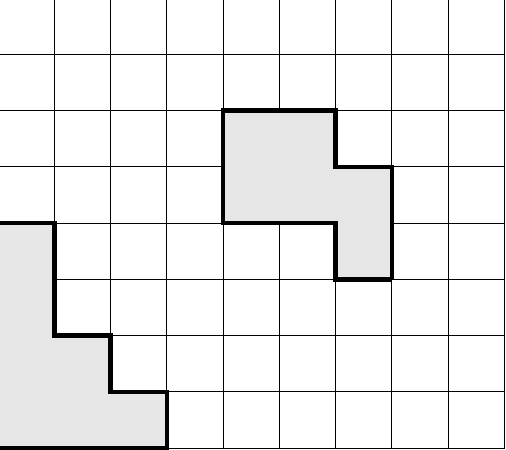
\includegraphics{pics/mask.pdf}%
  \end{picture}%
  \begin{picture}(300,264)(-9,461)
  \put(384,462){\makebox(0,0)[lb]{$i=\code{L}$}}
  \put(114,462){\makebox(0,0)[lb]{$i=1$}}
  \put( 93,477){\makebox(0,0)[lb]{$j=1$}}
  \put( 90,714){\makebox(0,0)[lb]{$j=\code{M}$}}
  \end{picture}
\caption{Small grid with masked regions}
\label{fmask}
\end{figure}
There are also arrays for the mask on $u$-points, $v$-points, and
$\psi$-points which are derived from the $\rho$-point mask.  The
$\psi$-point mask depends on the free-slip/no-slip option chosen
as described in \S\ref{Mask1}.

The programs in \code{gridpak} find the $\rho$-point mask based on the
bathymetry dataset.  Elevations at or above sea level are assumed to be
in the land mask.  You may choose to edit this mask, so Hernan Arango
has written a \code{Matlab} tool called \code{edit\_mask}.  It is an
interactive tool which requires \code{Matlab} as well as \code{mexnc}
for reading and writing NetCDF files from \code{Matlab}. On startup,
it will pop up file browsers, first for the grid file, then for a
coastline file. See Fig.\ \ref{fmat0} showing the file browser.

The view it presents is always rectangular, even for curvilinear grids,
but it will compute the coastline in the same (possibly) warped view to
allow a comparison. The first time you run it, it saves this mapped
coastline file to \code{ijcoast.mat} in the current directory.
Coastlines can be obtained from ...

\begin{figure}[pt]
  \setlength{\unitlength}{1 cm}%
  \begin{picture}(0,10)(0,0)%
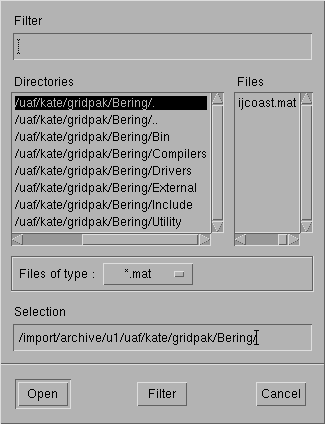
\includegraphics{pics/edit_mask0.png}
  \end{picture}
\caption{The \code{edit\_mask} file browser.}
\label{fmat0}
\end{figure}

An example of its use is shown in
Fig.\ \ref{fmat}, showing a Bering Sea grid.
It displays a rectangle for each $\rho$-point, including the
boundary ``image'' points.  The green/yellow boxes are land while the blue
ones are ocean. Figure \ref{fmat2} shows a zoomed in view where you
can actually see the individual boxes. Notice that scroll bars
appear automatically, allowing you to pan around.

Advice for masking details are as follows:
\begin{itemize}
  \item Make the ``image'' points have the same mask value as the points
they mirror. Something to avoid is an ocean image point adjacent
to a land point along an open boundary.
  \item Avoid one-grid bays such as the one that got away and is in
the right side of Fig.\ \ref{fmat2}. While these shouldn't cause the
model any direct grief, most plotting software cannot show you what
is happening in such places.
\end{itemize}

\begin{figure}[p]
  \setlength{\unitlength}{1 cm}%
  \begin{picture}(0,14)(0,0)%
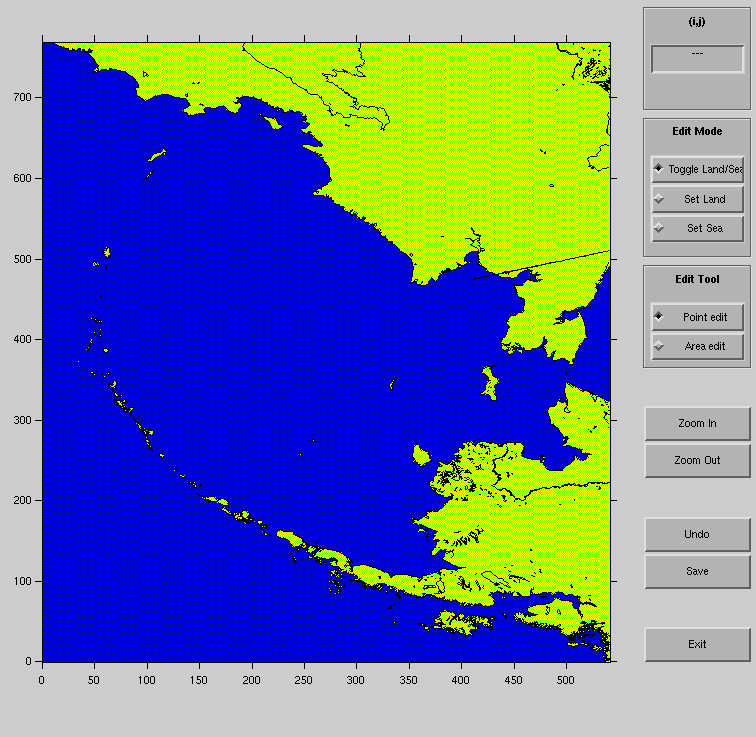
\includegraphics{pics/edit_mask1.png}
  \end{picture}
\caption{The \code{edit\_mask} program in action.}
\label{fmat}
\end{figure}

\begin{figure}[p]
  \setlength{\unitlength}{1 cm}%
  \begin{picture}(0,14)(0,0)%
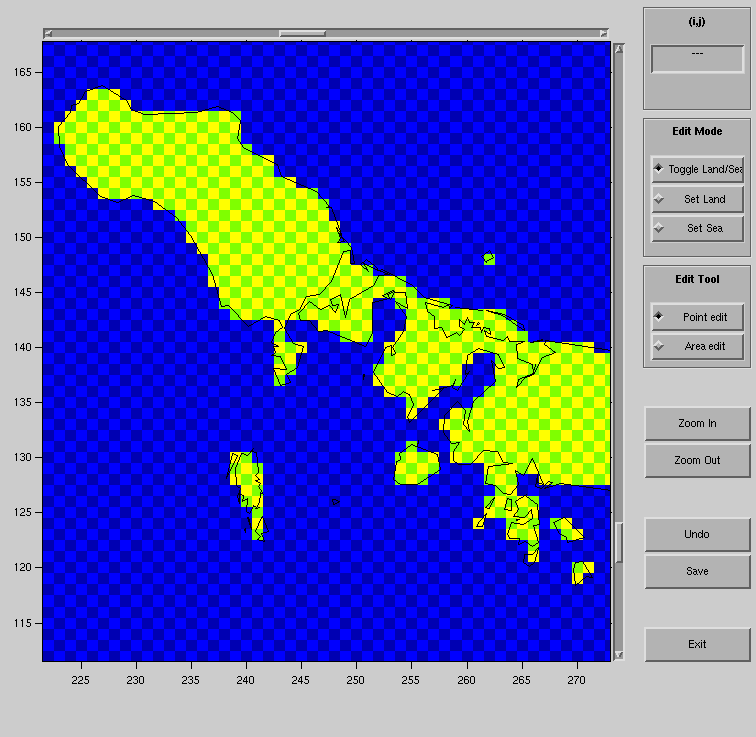
\includegraphics{pics/edit_mask2.png}
  \end{picture}
\caption{The \code{edit\_mask} program zoomed in.}
\label{fmat2}
\end{figure}

\subsection{Objective Analysis}
\label{OA}
[This section was contributed by Hernan Arango.]

The objective analysis (\code{oa}) package described here can be used
to prepare initial, climatology, update,  and forcing fields for SCRUM.
It maps oceanographic and atmospheric data to a specified application
grid.  Currently, it processes the following fields: {\sl in situ}
temperature, potential temperature, {\sl in situ} density anomaly,
salinity, sigma-t, sound speed, dynamic height, surface net heat flux
($Q$), surface freshwater flux, precipitation rate, evaporation rate,
incoming solar shortwave radiation, surface momentum (wind) stress
components, sea surface temperature (SST), and surface net heat flux
sensitivity to SST ($\partial Q / \partial {\rm SST}$).

This \code{oa} package is derived from an earlier program which Hernan
Arango and Carlos Lozano wrote at Harvard University in 1993.   The
basic algorithm used by this package is described in
\citet{Carter87}.  A comprehensive description of this
methodology can also be found in \citet{Gandin63,
Bretherton76, McWilliams86, Daley91, Bennett92}, and others.

Given observations $s_i = s({\bf x}_i, t_i)$ at location ${\bf x}_i,
t_i, i = 1, \ldots N$ an estimate $\phi_E$ of a scalar $\phi$ is
derived for location ${\bf x}$ and time $t$.  A linear unbiased estimate
is given by:
\[
   \phi_E({\bf x}, t) = \overline{\phi}({\bf x},t) + \sum_i w_i (s_i -
   \overline{s_i})
\]
for arbitrary $w_i$ since $\overline{\phi_E} = \overline{\phi}$.  The
associated variance of error is:
\[
  \overline{e^2(w)} = \overline{(\phi - \phi_E(w))^2}
\]
with $w = (w_1, \ldots w_N)$.  The overbar denotes an expected or
ensemble mean value.  The minimizer $w_*$:
\[
   \overline{e^2 (w_*)} \leq \overline{e^2(w)}
\]
is
\[
   w_* = {\bf A}^{-1} p
\]
with minimum error variance (Gauss-Markov):
\[
   \overline{e}^2_* = \overline{e^2(w_*)} = \overline{(\phi -
   \overline{\phi})^2} - p' {\bf A}^{-1} p
\]
Here, for convenience, matrix notation has been used.  $s = [s_1, \ldots
s_N]$ is a column correlation vector, $p = (\phi - \overline{\phi})(s
- \overline{s})$, and ${\bf A}$ is the covariance matrix:
\[
   {\bf A} = \overline{(s - \overline{s})(s - \overline{s})'}
\]
where the prime denotes a transpose.

Notice that ${\bf A}$ is symmetric.  In what follows, excluding
pathological cases, ${\bf A}$ is assumed to be positive definite.
The best linear estimate $\phi_*$ is then:
\[
   \phi_*({\bf x}, t) = \overline{\phi({\bf x}, t)} + p' {\bf A}^{-1}
   (s - \overline{s})
\]
with error $\overline{e^2_*}$.

The essential information required is statistical; namely the
spatial-temporal mean of the scalar and observations, the covariance
between observations, and the covariance between the scalar and the
observations.

The observations can be of different types, and different from the
scalar which you are trying to find.  Their usefulness is measured
by the fractional reduction of error:
\[
    {p'{\bf A}^{-1} p \over \overline{(\phi - \overline{\phi})^2}}
\]
In this package it is assumed that the covariance of the scalar is
homogeneous in space and homogeneous and isotropic in time:
\[
   C \left( ({\bf x_1}, t_1), ({\bf x_2}, t_2) \right) = 
   C \left( {\bf x_1 - x_2}, \left| t_2 - t_1 \right| \right)
\]
and errors at two different locations and times are uncorrelated:
\[
   E \left( ({\bf x}_1, t_1), ({\bf x}_2, t_2) \right) =
   E ({\bf x}_1, t_1) \delta ({\bf x_2 - x_1}) \delta(t_2 - t_1) .
\]
Currently, an analytical, isotropic, Gaussian correlation function is
assumed:
\[
    C({ \bf x_1 - x_2}, |t_2 - t_1| ) =
    {\cal C} ( |{ \bf x_1 - x_2}|, |t_2 - t_1| )
\]
with
\[
    {\cal C} ({\bf r}, \tau) = \exp \left[ - \left({\tau \over \tau_o}
    \right) ^2 \right] G({\bf r})
\]
\[
    G({\bf r}) = \left[ 1 - \left({{\bf r} \over a} \right)^2 \right]
    \exp \left[-\left({{\bf r} \over b} \right)^2 \right]
\]
where $\tau_o$ is the time decorrelation scale, $a$ is the zero
crossing distance, and $b$ is the spatial decorrelation scale.

This package uses a local solution to the \code{oa} equations.  That
is, only \code{nnce} influential observations are considered at each
mapped grid point.  This method is practical because it avoids
inverting large matrices when the number of observations is large.
Observations that are too far apart in space and time from the mapped
point contribute very little to the estimate, as one might expect.

\subsection{Forcing fields}
There are options for calling either \code{ana\_smflux} or
\code{get\_smflux} to get the surface momentum forcing.  If you do not
have an analytic formulation for this field,  you will have to create a
NetCDF forcing file which contains the surface momentum fluxes. This
file can be created with the \code{forcing} program, which reads the
output of the \code{oa} package.

The forcing file can
either contain one point value or a 2-D field of values.  Likewise, the
field can be constant in time or contain values for a series of times.
It is even possible to have a limited number of snapshots which get
cycled over in time.  For instance, you can provide 12 monthly mean
fields and tell it to cycle over these in a multi-year run.

The other forcing fields are treated in the same way and are also
contained in the NetCDF forcing file.  These include surface and bottom
heat and salt fluxes, the $\partial Q / \partial T$ and $T_{\rm ref}$
terms from \S\ref{vbc}, the incoming shortwave radiation used by the
Large et al.\ mixing scheme, and the wave information used by the
Styles and Glenn bottom boundary layer.  The ice thermodynamics also
requires forcing fields such as air temperature and cloud fraction.


\subsection{Initial and climatology fields}
The model will either read its initial fields from a NetCDF file or it
will compute them in \code{analytical.F}.  If it is not computing them,
the routine \code{get\_initial} will read a history file or a file
produced by the \code{initial} program.  This program in turn is
expecting to read the output of the \code{oa} program.

The model has the option of reading in 3-D climatology fields from a
climate NetCDF file.  This file contains the 3-D climatologies for the
tracers, perhaps at a number of times.  The subroutine \code{get\_clima}
will read this file and do any necessary time interpolations.  The
climate file is also produced by the \code{initial} program.  The
climatology could also be used for the boundary conditions, both for
the tracer values on inflow or for prescribed boundary conditions.  In
this case it would make more sense to only store the 2-D arrays.  We do
not yet have the software for handling these 2-D arrays, but it would
be a straightforward modification to the \code{initial} program.

%\include{floats}
\section{Ice Model Formulation}
\label{Iphys}

The sea-ice component of ROMS is a combination of the
elastic-viscous-plastic (EVP) rheology 
\citep{Hunke97,Hunke_2001} and simple one-layer
ice and snow thermodynamics with a molecular sublayer under the ice
\citep{Mellor89}. It is tightly coupled, having
the same grid (Arakawa-C) and timestep as the ocean and sharing the same
parallel coding structure for use with MPI or OpenMP \citep{Budgell05}.

\subsection{Dynamics}
The momentum equations describe the change in ice/snow velocity due
to the combined effects of the Coriolis force, surface ocean tilt,
air and water stress, and internal ice stress:
(\ref{ist1}) and (\ref{ist2}):
\begin{align}
  \frac{d}{ dt}(A \rho_i h_i u)
 & = A \rho_i h_i fv - A \rho_i h_i g \frac{\partial \zeta_w }{ \partial x} +
 A (\tau_a^x + \tau_w^x) + {\cal F}_x
\label{ist1} \\
  \frac{d}{ d t}(A \rho_i h_i v)
 & = - A \rho_i h_i fu - A \rho_i h_i g \frac{\partial \zeta_w }{ \partial y} +
 A (\tau_a^y + \tau_w^y) + {\cal F}_y.
\label{ist2}
\end{align}
In this model, we neglect the nonlinear advection terms as well as
the curvilinear terms in the internal ice stress.
Nonlinear formulae are used for both the ocean-ice and air-ice surface
stress:
\begin{align}
  \vec{\tau}_a & = \rho_a C_a | \vec{V}_{10} | \vec{V}_{10} \\
  C_a & = \frac{1 }{ 2} C_d \left[ 1 - \cos( 2 \pi \min(h_i+.1, .5)
  \right] \\
  \vec{\tau}_w & = \rho_w C_w | \vec{v}_w - \vec{v} |
  ( \vec{v}_w - \vec{v}) .
\end{align}
The force due to the internal ice stress is given by the divergence of
the stress tensor $\sigma$. The rheology is given by the stress-strain
relation of the medium. We would like to emulate the viscous-plastic
rheology of \citet{Hibler79}:
\begin{equation}
  \sigma_{ij} = 2 \eta \dot \epsilon_{ij} + (\zeta - \eta) \dot
  \epsilon_{kk} \delta_{ij} - \frac{P }{ 2} \delta_{ij}
\end{equation}
\begin{equation}
  \dot \epsilon_{ij} \equiv \frac{1 }{ 2} \left( \frac{\partial u_i
  }{
  \partial x_j} + \frac{\partial u_j }{ \partial x_i} \right)
\end{equation}
where the nonlinear viscosities are given by:
\begin{equation}
\zeta = \frac{ P }{ 2 \left[ (\epsilon^2_{11} +
   \epsilon^2_{22} ) ( 1 + 1/e^2 ) + 4 e^{-2} \epsilon^2_{12}
      + 2 \epsilon_{11} \epsilon_{22} ( 1 - 1/e^2 ) \right] ^{1/2} }
\end{equation}
\begin{equation}
      \eta = \frac{ \zeta }{ e^2 }.
\end{equation}
Hibler's ice strength is given by:
\begin{equation}
  P = P^* A h_i e^{-C(1-A)}
\end{equation}
while \citet{Overland_1988} advocate a nonlinear strength:
\begin{equation}
  P = P^* A h_i^2 e^{-C(1-A)}
\end{equation}
in which $P^*$ now depends on the grid spacing. Both options are available
in ROMS.

We would also like to have an explicit model that can be solved
efficiently on parallel computers. The EVP rheology has a tunable
coefficient $E$ (the Young's modulus) which can be chosen to make
the elastic term small compared to the other terms. We rearrange the VP
rheology:
\begin{equation}
  \frac{1 }{ 2 \eta} \sigma_{ij} + \frac{\eta - \zeta }{ 4 \eta \zeta}
  \sigma_{kk} \delta_{ij} + \frac{P }{ 4 \zeta} \delta_{ij} = \dot
  \epsilon_{ij}
\end{equation}
then add the elastic term:
\begin{equation}
  \frac{1 }{ E} \frac{\partial \sigma_{ij} }{ \partial t} +
  \frac{1 }{ 2
  \eta} \sigma_{ij} + \frac{\eta - \zeta }{ 4 \eta \zeta} \sigma_{kk}
  \delta_{ij} + \frac{P }{ 4 \zeta} \delta_{ij} = \dot \epsilon_{ij}
\end{equation}

Much like the ocean model, the ice model has a split timestep. The
internal ice stress term is updated on a shorter timestep so as to
allow the elastic wave velocity to be resolved.

Once the new ice velocities are computed, the ice tracers can be
advected using the MPDATA scheme \citep{Smolark90}. The tracers in
this case are the ice thickness, ice concentration, snow thickness,
internal ice temperature, and surface melt ponds. The continuity
equations describing the evolution of these parameters (equations
(\ref{ist3a})--(\ref{ist3b})) also include thermodynamic terms ($S_h$,
$S_s$ and $S_A$), which will be described in \S\ref{Growth}:
\begin{align}
  \frac{\partial A h_i }{ \partial t} & =
  - \frac{\partial (u A h_i) }{ \partial x} -
  \frac{\partial (v A h_i) }{ \partial y}
  + S_h + {\cal D}_h
\label{ist3a} \\
  \frac{\partial A h_s }{ \partial t} & =
  - \frac{\partial (u A h_s) }{ \partial x} -
  \frac{\partial (v A h_s) }{ \partial y}
  + S_s + {\cal D}_s
\label{ist3c} \\
  \frac{\partial A }{ \partial t} & =
  - \frac{\partial (uA) }{ \partial x} - \frac{\partial (vA) }{ \partial y}
  + S_A + {\cal D}_A \qquad \qquad 0 \leq A \leq 1 .
\label{ist3b}
\end{align}
The first two equations represent the conservation of ice and snow.
Equation (\ref{ist3b}) is discussed in some detail in \citet{Mellor89}, but
represents the advection of ice blocks in which no ridging occurs as
long as there is any open water.
%An optional ridging term can be added
%\citep{Gray96}:
%\begin{equation}
%  \frac{\partial A }{ \partial t} =
%  - \frac{\partial (uA) }{ \partial x} - \frac{\partial (vA) }{ \partial y}
%  - A \alpha(A) \, \nabla \cdot \vec{v} \, H(-\nabla \cdot \vec{v})
%  + S_A + {\cal D}_A \qquad \qquad 0 \leq A \leq 1 .
%\end{equation}
%where $\alpha(A)$ is an arbitrary function such that $\alpha(0) = 0$,
%$\alpha(1) = 1$, and $0 \leq \alpha(A) \leq 1$. The ridging term leads
%to an increase in $h_i$ under convergent flow as would be produced by
%ridging. The function $\alpha(A)$ should be chosen so that it is near
%zero until the ice concentration is large enough that ridging is
%expected to occur, then should increase smoothly to one.
%
The symbols used in these equations along with the values for the
constants are listed in Table \ref{icemomvars}.

\begin{table}[pt]
\hspace{9.5 mm}
\vbox{
\begin{tabular}{|c|c|l|} \hline
  Variable & Value & Description \\ \hline
  $A(x,y,t)$ && ice concentration \\
%  $\alpha(A)$ && ridging function \\
  $C_a$ && nonlinear air drag coefficient \\
  $C_d$ & $2.2 \times 10^{-3}$ & air drag coefficient \\
  $C_w$ & $10 \times 10^{-3}$ & water drag coefficient \\
  (${\cal D}_h, {\cal D}_s, {\cal D}_A$) && diffusion terms \\
  $\delta_{ij}$ && Kronecker delta function \\
  $E$ && Young's modulus \\
  $e$ & 2 & eccentricity of the elliptical yield curve \\
  $\epsilon_{ij}(x,y,t)$ && strain rate tensor \\
  $\eta(x,y,t)$ && nonlinear shear viscosity \\
  $f(x,y)$ && Coriolis parameter \\
  (${\cal F}_x, {\cal F}_y$) && internal ice stress \\
  $g$  & $9.8\, m\, s^{-2}$ & acceleration of gravity \\
  $H$ &&  Heaviside function \\
  $h_i(x,y,t)$ && ice thickness of ice-covered fraction \\
  $h_o$ & 1 m & ice cutoff thickness \\
  $h_s(x,y,t)$ && snow thickness on ice-covered fraction \\
  $M(x,y,t)$ && ice mass (density times thickness) \\
  $P(x,y,t)$ && ice pressure or strength \\
  ($P^*, C$) & ($2.75 \times 10^4, 20$) & ice strength parameters \\
  ($S_h, S_s, S_A$) && thermodynamic terms \\
  $\sigma_{ij}(x,y,t)$ && stress tensor \\
  $\vec{\tau}_a$ && air stress \\
  $\vec{\tau}_w$ && water stress \\
  ($u,v$) && the ($x,y$) components of ice velocity $\vec{v}$ \\
  ($\vec{V}_{10}, \vec{v}_w$) &&
	      10 meter air and surface water velocities \\
  ($\rho_a, \rho_w$)  & ($1.3\, kg\, m^{-3}, 1025\, kg\, m^{-3}$) & air
  and water densities \\
  $\zeta(x,y,t)$ && nonlinear bulk viscosity \\
  $\zeta_w(x,y,t)$ && height of the ocean surface \\
  \hline
\end{tabular}
}
\caption{Variables used in the ice momentum equations.}
\label{icemomvars}
\end{table}

Note that Hibler's $h_I$ variable is equivalent to our $A h_i$
combination - his $h_I$ is the average thickness over the whole
gridbox while our $h_i$ is the average thickness over the ice-covered
fraction of the gridbox. 

\subsubsection{Landfast ice}
\label{Landfast_ice}

The Arctic ocean has many shallow shelves, on which landfast ice
can form every winter. The model as described thus far has no way to
reproduce the landfast ice, but \citet{Lemieux_2015} describes a
landfast ice parameterization. Basal stress terms $\tau_b$ are added to
equations (\ref{ist1}) and (\ref{ist2}) representing a bottom drag
applied to the deepest ice keels. Included is a parameterization of the
ice thickness distribution so that even a single ice-category model can
use the landfast ice option. Figure \ref{f_landfast} shows a cartoon of
an ice floe with a keel.

\begin{figure}[ht]

\begin{center}
\definecolor{cc87137}{RGB}{200,113,55}
\definecolor{c2ad4ff}{RGB}{42,212,255}
\definecolor{c55ddff}{RGB}{85,221,255}
\definecolor{c0072ff}{RGB}{0,114,255}


\begin{tikzpicture}[y=0.80pt, x=0.80pt, yscale=-1.000000, xscale=1.000000, inner sep=0pt, outer sep=0pt]
\begin{scope}[shift={(0,-485.43307)}]
  \path[fill=cc87137,rounded corners=0.0000cm] (149.3704,752.5492) rectangle
    (449.3704,772.5492);
  \path[draw=c2ad4ff,fill=c55ddff,line join=miter,line cap=butt,even odd rule,line
    width=0.800pt] (150.0000,602.3622) -- (150.0000,622.3622) --
    (250.0000,622.3622) -- (260.0000,741.9196) -- (270.0000,622.3622) --
    (360.0000,622.3622) -- (360.0000,602.3622) -- (270.0000,602.3622) --
    (260.0000,592.3622) -- (250.0000,602.3622) -- cycle;
  \path[draw=c0072ff,line join=miter,line cap=butt,miter limit=4.00,even odd
    rule,line width=1.600pt] (360.0000,606.7695) .. controls (365.0000,606.7695)
    and (374.1050,600.8756) .. (377.6873,601.0614) .. controls (381.2696,601.2471)
    and (379.9588,603.7348) .. (395.6076,607.9057) .. controls (406.2484,608.4328)
    and (407.0792,603.2019) .. (417.7482,602.1621) .. controls (430.6436,599.4896)
    and (427.8328,609.1786) .. (441.1189,609.7014) .. controls (452.2796,609.3679)
    and (447.9592,604.7616) .. (458.6417,600.6002) .. controls (461.0764,598.8109)
    and (473.4825,605.7417) .. (472.3709,604.8806);
  \path[draw=c0072ff,line join=miter,line cap=butt,miter limit=4.00,even odd
    rule,line width=1.600pt] (150.0000,604.2510) .. controls (148.3100,605.5942)
    and (142.4698,606.3718) .. (140.0415,606.6003) .. controls (125.5603,609.5491)
    and (124.8491,595.8552) .. (116.5882,605.9987) .. controls (111.6403,609.6048)
    and (104.8953,602.7983) .. (99.3704,605.4365);
\end{scope}
  \path[draw=black,dash pattern=on 2.40pt off 0.80pt,line join=miter,line
    cap=butt,miter limit=4.00,even odd rule,line width=0.800pt] (150.0000,35.4486)
    -- (150.0000,95.5276);
  \path[draw=black,dash pattern=on 2.40pt off 0.80pt,line join=miter,line
    cap=butt,miter limit=4.00,even odd rule,line width=0.800pt] (450.0000,36.7078)
    -- (450.0000,98.0460);
  \path[->,>=stealth,draw=black,line join=miter,line cap=butt,even odd rule,line width=0.800pt]
    (280.8509,47.3375) -- (150.6296,47.3375);
  \path[->,>=stealth,draw=black,line join=miter,line cap=butt,even odd rule,line width=0.800pt]
    (280.2213,76.7816) -- (150.6296,76.7816);
  \path[->,>=stealth,draw=black,line join=miter,line cap=butt,even odd rule,line width=0.800pt]
    (296.0000,77.4112) -- (360.5953,77.4112);
  \path[->,>=stealth,draw=black,line join=miter,line cap=butt,even odd rule,line width=0.800pt]
    (308.0000,47.3375) -- (450.0000,47.3375);
  \path[->,>=stealth,draw=black,line join=miter,line cap=butt,even odd rule,line width=0.800pt]
    (280.0000,186.9291) -- (280.0000,136.9291);
  \path[->,>=stealth,draw=black,line join=miter,line cap=butt,even odd rule,line width=0.800pt]
    (280.0000,206.9291) -- (280.0000,256.9291);
  \path[->,>=stealth,draw=black,line join=miter,line cap=butt,even odd rule,line width=0.800pt]
    (210.0000,86.9291) -- (210.0000,116.9291);
  \path[->,>=stealth,draw=black,line join=miter,line cap=butt,even odd rule,line width=0.800pt]
    (210.0000,166.9291) -- (210.0000,136.9291);
  \path[->,>=stealth,draw=black,line join=miter,line cap=butt,even odd rule,line width=0.800pt]
    (250.0000,86.9291) -- (250.0000,106.9291);
  \path[->,>=stealth,draw=black,line join=miter,line cap=butt,even odd rule,line width=0.800pt]
    (250.0000,146.9291) -- (250.0000,116.9291);
  \path[->,>=stealth,draw=black,line join=miter,line cap=butt,even odd rule,line width=0.800pt]
    (360.0000,86.9291) -- (361.2592,120.0034);
  \path[->,>=stealth,draw=black,line join=miter,line cap=butt,even odd rule,line width=0.800pt]
    (360.0000,166.9291) -- (360.0000,136.9291);
  \path[->,>=stealth,draw=black,line join=miter,line cap=butt,even odd rule,line width=0.800pt]
    (149.6707,180.0034) -- (149.6707,120.5593);
  \path[->,>=stealth,draw=black,line join=miter,line cap=butt,even odd rule,line width=0.800pt]
    (149.7818,197.4850) -- (150.4114,265.7437);
  \path[->,>=stealth,draw=black,line join=miter,line cap=butt,even odd rule,line width=0.800pt]
    (210.0000,86.9291) -- (210.0000,116.9291);
  \path[->,>=stealth,draw=black,line join=miter,line cap=butt,even odd rule,line width=0.800pt]
    (210.0000,166.9291) -- (210.0000,136.9291);
  \path[->,>=stealth,draw=black,line join=miter,line cap=butt,even odd rule,line width=0.800pt]
    (250.0000,86.9291) -- (250.0000,106.9291);
  \path[->,>=stealth,draw=black,line join=miter,line cap=butt,even odd rule,line width=0.800pt]
    (250.0000,146.9291) -- (250.0000,116.9291);
  \path[->,>=stealth,draw=black,line join=miter,line cap=butt,even odd rule,line width=0.800pt]
    (360.0000,86.9291) -- (361.2592,120.0034);
  \path[->,>=stealth,draw=black,line join=miter,line cap=butt,even odd rule,line width=0.800pt]
    (360.0000,166.9291) -- (360.0000,136.9291);
  \path[->,>=stealth,draw=black,line join=miter,line cap=butt,even odd rule,line width=0.800pt]
    (219.2597,121.9665) -- (249.2597,121.9665);
  \path[->,>=stealth,draw=black,line join=miter,line cap=butt,even odd rule,line width=0.800pt]
(302.1470,121.8554) -- (272.1470,121.8554);

  \path[fill=black,line join=miter,line cap=butt,line width=0.800pt]
    (269.3704,202.5219) node[above right] (text7731) {$h_{rb}$};
  \path[fill=black,line join=miter,line cap=butt,line width=0.800pt]
    (362.4447,135.0403) node[above right] (text7735) {$h_d$};
  \path[fill=black,line join=miter,line cap=butt,line width=0.800pt]
    (283.7776,52.5219) node[above right] (text7739) {$\Delta x$};
  \path[fill=black,line join=miter,line cap=butt,line width=0.800pt]
    (284.4073,80.6330) node[above right] (text7743) {$l_i$};
  \path[fill=black,line join=miter,line cap=butt,line width=0.800pt]
    (143.1481,194.4107) node[above right] (text7747) {$h_w$};
  \path[fill=black,line join=miter,line cap=butt,line width=0.800pt]
    (193.1481,108.8180) node[above right] (text7751) {$h_l$};
  \path[fill=black,line join=miter,line cap=butt,line width=0.800pt]
    (231.8888,113.1515) node[above right] (text7755) {$h_{rt}$};
  \path[fill=black,line join=miter,line cap=butt,line width=0.800pt]
    (254.3626,127.4611) node[above right] (text4378) {$\beta l_i$};
\end{tikzpicture}
\caption{Cartoon of an ice floe with a deep keel.}
\label{f_landfast}
\end{center}
\end{figure}

\begin{table}[pt]
\begin{center}
%\hspace{9.5 mm}
\vbox{
\begin{tabular}{|c|c|l|} \hline
  Variable & Value & Description \\ \hline
  $h_w$ && water depth \\
  $h_{rt}$ && ridge height above level ice \\
  $h_{rb}$ && draft of keels below level ice bottom \\
  $h_d$ && draft of ice below sea surface \\
  $l_i$ && length of ice floe within grid cell \\
  $\Delta x$ && $x$-dimension of grid cell \\
  $\beta$ & O(0.01) & ridged fraction of floe \\
  $k_1$ & 8.0 & tunable parameter \\
  $k_2$ & 15.0 & tunable parameter \\
  $u_0$ & $5.0\times 10^{-5}$ & small velocity \\
  $C_b$ & 20 & ice strength parameter \\
  \hline
\end{tabular}
}
\end{center}
\caption{Variables used in the landfast ice parameterization.}
\label{fasticevars}
\end{table}

Introducing the tunable parameters $k_1$ and $k_2$, plus the
expression $h_c = A h_w/k_1$, the $u$-component of the basal
stress due to the dragging of ice keels is computed as:
\begin{equation}
  \tau_{bu} = 
    \begin{cases}
      0& \text{if $h_w \geq h_c$},\\
      k_2 \left( \frac{u}{|\vec{v}| + u_0} \right)
            (h_w-h_c)\exp^{-C_b(1-A)}& \text{if $h_w < h_c$}.
    \end{cases}
\end{equation}
where $h_w$ is the water depth.
The expression for the $v$-component is similar.

\subsection{Thermodynamics}
\label{Growth}

The thermodynamics is based on calculating how much ice grows and
melts on each of the surface, bottom, and sides of the ice floes,
as well as frazil ice formation \citep{Mellor89}.
Once the ice tracers are advected, the ice concentration and
thickness are timestepped according to the terms on the right.

Equations (\ref{ist3a}) and (\ref{ist3b}) become:
\begin{align}
  \frac{D A h_i }{D t}
  & = \frac{\rho_o }{ \rho_i} \left[ A (W_{io} - W_{ai}) + (1-A) W_{ao}
  + W_{fr} \right]
\label{ist4a} \\
  \frac{D A }{ D t}
  & = \frac{\rho_o}{ \rho_i h_i} \left[ \Phi (1-A) W_{ao} + (1-A)
  W_{fr} \right] \qquad \qquad 0 \leq A \leq 1 .
\label{ist4b}
\end{align}
The term $Ah_i$ is the ``effective thickness'', a measure of the ice
volume. Its evolution equation is simply quantifying the change in
the amount of ice. The ice concentration equation is more interesting in
that it provides the partitioning between ice melt/growth on the sides
vs. on the top and bottom. The parameter $\Phi$ controls this and has
differing values for ice melt and retreat. In principle, most of the ice
growth is assumed to happen at the base of the ice while rather more of
the melt happens on the sides of the ice due to warming of the water in
the leads.

The heat fluxes through the ice are based on a simple one layer
\citet{Semtner76a} type model with snow on top. The temperature is
assumed to be linear within the snow and within the ice. The ice contains
brine pockets for a total ice salinity of 3.2 or the surface salinity,
whichever is less. The surface ocean temperature and salinity is half a
$dz$ below the surface. The water right below the surface is assumed to
be at the freezing temperature; a logarithmic boundary layer is computed
having the temperature and salinity matched at freezing.

Here, the $W$ variables are the freeze or
melt rates as shown in Fig.\ \ref{fm+k} and Table \ref{thermvar}.  The
frazil ice growth $W_{fr}$ will be discussed further in
\S\ref{frazil}---note that it contributes to changes in $A$ as well as
to changes in $h_i$.  The other term that contributes to $A$ is
$W_{ao}$.  This term includes a factor $\Phi$ which Mellor and Kantha
set to different values depending on whether ice is melting or
freezing:
\begin{align}
    \Phi & = 4.0 \qquad\qquad W_{ao} \geq 0 \\
    \Phi & = 0.5 \qquad\qquad W_{ao} < 0
\end{align}

\begin{figure}[ht]
\setlength{\unitlength}{0.00083300in}%
%
%\begin{picture}(6527,2507)(270,-5042)
\begin{picture}(6591,3076)(835,-5072)
%\thicklines
\put(1501,-2911){\line( 1, 0){3975}}
\put(1501,-4111){\line( 1, 0){3975}}
\put(1501,-2911){\line( 0,-1){1200}}
\put(6976,-4111){\line( 1, 0){1050}}
\put(6976,-2941){\line( 1, 0){1050}}
\put(6976,-2711){\line( 0,-1){1400}}
\put(6976,-2711){\line( 1, 0){1050}}
\put(5476,-2911){\line( 0,-1){1200}}
\put(2401,-4811){\vector( 0, 1){700}}
\put(3376,-4861){\vector( 0, 1){750}}
\put(6226,-3586){\vector( 0, 1){675}}
\put(4426,-4036){\vector( 0,-1){525}}
\put(2596,-3376){\vector( 1, 1){450}}
\put(7526,-2211){\vector( 0,-1){500}}
\put(7490,-3383){\vector( 1,2){200}}
\put(6121,-3786){\makebox(0,0)[lb]{$W_{ao}$}}
\put(4336,-4756){\makebox(0,0)[lb]{$W_{ro}$}}
\put(2416,-3586){\makebox(0,0)[lb]{$W_{ai}$}}
\put(3241,-5056){\makebox(0,0)[lb]{$W_{io}$}}
\put(2296,-5056){\makebox(0,0)[lb]{$W_{fr}$}}
\put(7400,-2180){\makebox(0,0)[lb]{$W_{s}$}}
\put(7276,-3611){\makebox(0,0)[lb]{$W_{sm}$}}
\end{picture}
%\begin{picture}(0,0)(5346,0)
\begin{picture}(0,0)(5961,-30)
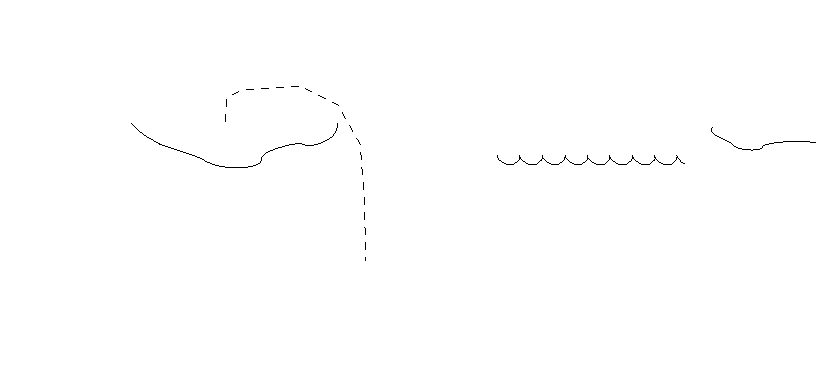
\includegraphics{pics/therm_mk}%
\end{picture}%
\caption{Diagram of the different locations where ice melting and
freezing can occur.}
\label{fm+k}
\end{figure}

Similar to Eq. (\ref{ist4a}) is the snow equation:
\begin{equation}
  {D A h_s \over D t} = \left[ A (W_{s} - W_{sm}) \right]
\end{equation}
where $W_s$ and $W_{sm}$ are the snowfall and snow melt rates,
respectively, in units of equivalent water. Currently all snow and
ice melt ends up in $W_{ro}$, though melt ponds could be added with
some effort.

\begin{table}
\hspace{9 mm}
\vbox{
\begin{tabular}{|c|c|l|} \hline
  Variable & Value & Description \\ \hline
  $\alpha_w$ & 0.10 & shortwave albedo of water \\
  $\alpha_i$ & 0.60, 0.65 & shortwave albedo of wet, dry ice \\
  $\alpha_s$ & 0.72, 0.85 & shortwave albedo of wet snow \\
  $C_k$ && snow correction factor \\
  $C_{pi}$ & 2093 J kg$^{-1}$ K$^{-1}$ & specific heat of ice \\
  $C_{po}$ & 3990 J kg$^{-1}$ K$^{-1}$ & specific heat of water \\
  $\epsilon_w$ & 0.97 & longwave emissivity of water \\
  $\epsilon_i$ & 0.97 & longwave emissivity of ice \\
  $\epsilon_s$ & 0.99 & longwave emissivity of snow \\
  $E(T,r)$ && enthalpy of the ice/brine system \\
  $F_T\!\uparrow$ && heat flux from the ocean into the ice \\
  $h^\star$ && test for thick snow pushing ice surface under water \\
  $H\!\downarrow$ && sensible heat \\
  $I_o$ & part of $(1-\alpha_i)SW\!\!\downarrow$ & shortwave radiation entering ice \\
  $i_w$ && fraction of the solar heating transmitted \\
  && through a lead into the water below \\
  $k_i$ & 2.04 W m$^{-1}$ K${^-1}$ & thermal conductivity of ice \\
  $k_s$ & 0.31 W m$^{-1}$ K${^-1}$ & thermal conductivity of snow \\
  $L_i$ & 302 MJ m$^{-3}$ & latent heat of fusion of ice \\
  $L_s$ & 110 MJ m$^{-3}$ & latent heat of fusion of snow \\
  $LE\!\downarrow$ && latent heat \\
  $LW\!\!\downarrow$ && incoming longwave radiation \\
  $m$ & $-0.054^\circ$C & coefficient in linear $T_f(S) = mS$ equation \\
  $\Phi$ && contribution to $A$ equation from freezing water \\
  $Q_{ai}$ && heat flux out of the snow/ice surface \\
  $Q_{ao}$ && heat flux out of the ocean surface \\
  $Q_{i2}$ && heat flux up out of the ice \\
  $Q_{io}$ && heat flux up into the ice \\
  $Q_{s}$  && heat flux up through the snow \\
  $r$   & $0 \le r \le 0.2 $ & brine fraction in ice \\
  $\rho_i$ & 910 $m^3/kg$ & density of ice \\
  $S_i$ & 3.2 & salinity of the ice \\
  $SW\!\!\downarrow$ && incoming shortwave radiation \\
  $\sigma$ & $5.67 \times 10^{-8}$ W m$^{-2}$ K$^{-4}$ &
  Stefan-Boltzmann constant \\
  $T_0$ && temperature of the bottom of the ice \\
  $T_1$ && temperature of the interior of the ice \\
  $T_2$ && temperature at the upper surface of the ice \\
  $T_3$ && temperature at the upper surface of the snow \\
  $T_f$ && freezing temperature \\
  $T_{{\rm melt}\_i}$ & $mS_i$ & melting temperature of ice \\
  $T_{{\rm melt}\_s}$ & 0$^\circ$ C & melting temperature of snow \\
  $W_{ai}$ && melt rate on the upper ice/snow surface \\
  $W_{ao}$ && freeze rate at the air/water interface \\
  $W_{fr}$ && rate of frazil ice growth \\
  $W_{io}$ && freeze rate at the ice/water interface \\
  $W_{ro}$ && rate of run-off of surface melt water \\
  $W_{s}$  && snowfall rate \\
  $W_{sm}$ && snow melt rate \\
  \hline
\end{tabular}
}
\caption{Variables used in the ice thermodynamics}
\label{thermvar}
\end{table}

\begin{figure}
\centerline{
\begin{picture}(0,0)%
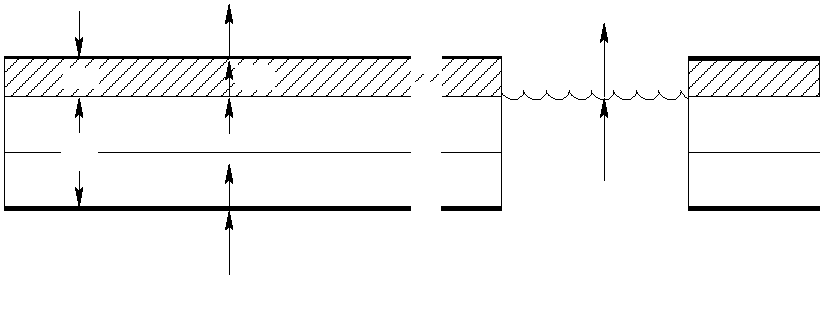
\includegraphics{pics/therm_mk2}%
\end{picture}%
\setlength{\unitlength}{3947sp}%
%
\begin{picture}(6591,2608)(1468,-5057)
\put(6376,-3511){\makebox(0,0)[lb]{{$F_T$}}}
\put(3376,-4561){\makebox(0,0)[lb]{{$F_T$}}}
\put(3376,-4036){\makebox(0,0)[lb]{{$Q_{io}$}}}
\put(3376,-3436){\makebox(0,0)[lb]{{$Q_{i2}$}}}
\put(6376,-3061){\makebox(0,0)[lb]{{$Q_{ao}$}}}
\put(3376,-3136){\makebox(0,0)[lb]{{$Q_s$}}}
\put(3376,-2761){\makebox(0,0)[lb]{{$Q_{ai}$}}}
\put(2026,-3736){\makebox(0,0)[lb]{{$h_i$}}}
\put(2026,-3136){\makebox(0,0)[lb]{{$h_s$}}}
\put(4801,-4186){\makebox(0,0)[lb]{{$T_0$}}}
\put(4801,-2986){\makebox(0,0)[lb]{{$T_3$}}}
\put(4801,-3286){\makebox(0,0)[lb]{{$T_2$}}}
\put(4801,-3736){\makebox(0,0)[lb]{{$T_1$}}}
\end{picture}
}
\caption{Diagram of internal ice temperatures and fluxes. The hashed
layer is the snow.}
\label{fflux}
\end{figure}

Figure \ref{fflux} shows the locations of the ice and snow temperatures
and the heat fluxes. The temperature profile is assumed to be linear
between adjacent temperature points. The interior of the ice contains
``brine pockets'', leading to a prognostic equation for the temperature
$T_1$.

The surface flux to the air is:
\begin{equation}
   Q_{ai} =  - H\!\downarrow - LE\!\downarrow -
       \epsilon_s LW\!\!\downarrow  -
      (1 - \alpha_s) SW\!\!\downarrow + \epsilon_s \sigma (T_3+273)^4
\end{equation}
The incoming shortwave and longwave radiations are assumed to
come from an atmospheric model. The formulae for sensible heat,
latent heat, and outgoing longwave radiation are the same as in
\citet{Parkinson} and are shown in Appendix
\ref{shortwave}. The sensible heat is a function of $T_3$, as is the
heat flux through the snow $Q_s$. Setting $Q_{ai} = Q_s$, we can solve
for $T_3$ by setting $T_3^{n+1} = T_3^n + \Delta T_3$ and linearizing in
$\Delta T_3$. As in Parkinson and Washington, if $T_3$
is found to be above the melting temperature, it is set to $T_{\rm melt}$
and the extra energy goes into melting the snow or ice:
\begin{align}
   W_{ai} & = \frac{Q_{ai} - Q_{i2} }{ \rho_o L_3} \label{eqWai} \\
   L_3 & \equiv \left[ E(T_3,1) - E(T_1, r) \right]
\end{align}
Note that $L_3 = (1-r)L_i$ plus a small sensible heat correction.

If there is no snow, there is an option to allow some of the incoming
shortwave radiation ($I_o = 0.17(1-\alpha_i)SW\!\!\downarrow$) to
enter the ice and contribute to heating up the ice rather than to
melting the surface ice \citep{Maykut71}. It essentially reduces $Q_{i2}$
by the amount $I_o$ in both equations (\ref{eqWai}) and (\ref{eqdEdt}).

%We can store water on the surface in melt pools to a fixed
%depth---everything extra melted at the surface is assumed to flow into
%the ocean as $W_{ro}$. The melt ponds however do not contribute to
%the heat flux computation.

Inside the ice there are brine pockets in which there is salt water
at the {\it in situ} freezing temperature. It is assumed that the ice
has a uniform overall salinity of $S_i$ and that the freezing
temperature is a linear function of salinity. The brine fraction $r$ is
given by
$$
  r = \frac{S_i m }{ T_1}
$$
The enthalpy of the combined ice/brine system is given by
\begin{equation}
  E(T,r) = r(L_i + C_{po}T) + (1-r) C_{pi} T
\end{equation}
Substituting in for $r$ and differentiating gives:
\begin{equation}
  \frac{\partial E }{ \partial T_1} = - \frac{S_i m L_i }{ T_1^2} + C_{pi}
\end{equation}

Inside the snow, we have
\begin{equation}
   Q_s = \frac{k_s }{ h_s} (T_2 - T_3)
\end{equation}
The heat conduction in the upper part of the ice layer is
\begin{equation}
   Q_{I2} = \frac{ 2 k_i }{ h_i} (T_1 - T_2)
   \label{qi2}
\end{equation}
These can be set equal to each other to solve for $T_2$
\begin{equation}
   T_2 = \frac{T_3 + C_k T_1 }{ 1 + C_k}
\end{equation}
where
$$
  C_k \equiv \frac{2 k_i h_s }{ h_i k_s}.
$$
Substituting into (\ref{qi2}), we get:
\begin{equation}
  Q_s = Q_{I2} = \frac{2k_i }{ h_i} \frac{(T_1 - T_3) }{ (1 + C_k)}
\label{qsnow}
\end{equation}
Note that in the absence of snow, $C_k$ becomes zero and we recover the
formula for the no-snow case in which $T_3 = T_2$.

At the bottom of the ice, we have
\begin{equation}
  Q_{I0} = \frac{2 k_i }{ h_i} (T_0 - T_1)
\end{equation}
The difference between $Q_{I0}$ and $Q_{I2}$ goes into the enthalpy of
the ice:
\begin{equation}
   \rho_i h_i \left[ \frac{\partial E }{ \partial t} + \vec{v} \cdot 
   \nabla E \right] = Q_{I0} - Q_{I2}
  \label{eqdEdt}
\end{equation}
We can use the chain rule to obtain an equation for timestepping $T_1$:
\begin{equation}
   \rho_i h_i \frac{\partial E }{ \partial T_1}
   \left[ \frac{\partial T_1 }{ \partial t} + \vec{v} \cdot 
   \nabla T_1 \right] = Q_{I0} - Q_{I2}
\end{equation}
where
\begin{align*}
  Q_{I0} - Q_{I2} & = \frac{2 k_i }{ h_i} \left[ (T_0 - T_1) - 
  \frac{(T_1 - T_3) }{ 1 + C_k} \right] \\
	          & = \frac{2 k_i }{ h_i} \left[ (T_0 +
  \frac{T_3 - (2 + C_k) T_1 }{ 1 + C_k} \right]
\end{align*}

When the snow gets thick enough, it pushes the ice down to the point
where seawater floods onto the ice where it can possibly refreeze.
The condition for such thick snow is $h^\star > 0$, where
\begin{equation}
    h^\star = h_s - \frac{(\rho_w - \rho_i)}{\rho_s} h_i
\end{equation}
An optional model process is to convert the thick snow into ice
directly:
\begin{align}
    h_s & = h_s - \frac{\rho_i h^\star}{\rho_w} \\
    h_i & = h_i + \frac{\rho_s h^\star}{\rho_w}
\end{align}

\subsubsection{Ocean surface boundary conditions}
The ocean receives surface stresses from both the atmosphere and the
ice, according to the ice concentration:
\begin{align}
   K_m \frac{\partial u_w }{ \partial z} & = \frac{A }{ \rho_o} \tau_{io}^x
    + \frac{1-A }{ \rho_o} \tau_{ao}^x \\
   K_m \frac{\partial v_w }{ \partial z} & = \frac{A }{ \rho_o} \tau_{io}^y
    + \frac{1-A }{ \rho_o} \tau_{ao}^y
\end{align}
where the relevant variables are in Table \ref{tobc}.

\begin{table}
\hspace{35 mm}
\vbox{
\begin{tabular}{|c|c|l|} \hline
Variable & Value & Definition \\ \hline
   $b$ & 3.14 & factor \\
   \.E && evaporation \\
   $k$ & 0.4 & von Karman's constant \\
   $K_m$ && vertical viscosity of seawater \\
   $\nu$ & $1.8 \times 10^{-6} m^2 s^{-1}$ &
      kinematic viscosity of seawater \\
   \.P && precipitation \\
   $Pr$ & 13.0 & molecular Prandtl number \\
   $P_{rt}$ & 0.85 & turbulent Prandtl number \\
   $S$ && internal ocean salinity \\
   $S_0$ && surface salinity \\
   $Sc$ & 2432.0 & molecular Schmidt number \\
   $\tau_{io}$ && stress on the ocean from the ice \\
   $\tau_{ao}$ && stress on the ocean from the wind \\
   $T$ && internal ocean temperature \\
   $T_0$ && surface temperature \\
   $u_\tau$ && friction velocity $|\tau_{io}|^{1/2} \rho_o^{-1/2}$ \\
   $z_0$ && roughness parameter \\
  \hline
\end{tabular}
}
\caption{Ocean surface variables}
\label{tobc}
\end{table}

The surface ocean is assumed to be at the freezing temperature for the
surface salinity ($T_0 = mS_0$) in the presense of ice. We also have $T$ and $S$ at the
uppermost computed ocean point ${1 \over 2} dz$ below the surface.
In order to solve for $T_0$ and $S_0$, we assume a \citep{Yaglom_1974}
logarithmic boundary layer. The upper ocean heat flux is:
\begin{equation}
   \frac{F_T }{ \rho_o C_{po}} = -C_{T_z} (T_0 - T) \qquad z \rightarrow 0
\end{equation}
where
\begin{gather}
  C_{T_z} = \frac{u_\tau }{ P_{rt} k^{-1}\ln (-z/z_0) + B_T} \\
  B_T = b \left(\frac{z_0 u_\tau }{ \nu} \right) ^{1/2} Pr^{2/3}
\end{gather}
Likewise, we have the following equation for the surface salt flux:
\begin{equation}
   F_S = -C_{S_z} (S_0 - S) \qquad z \rightarrow 0
\end{equation}
where
\begin{gather}
  C_{S_z} = \frac{u_\tau }{ P_{rt} k^{-1}\ln (-z/z_0) + B_S} \\
  B_S = b \left(\frac{z_0 u_\tau }{ \nu} \right) ^{1/2} Sc^{2/3}
\end{gather}

The ocean model receives the following heat and salt fluxes:
\begin{align}
   F_T & = A Q_{io} + (1 - A) Q_{ao} - W_o L_o \\
   F_S & = (W_o - A W_{ro}) (S_i-S_0) + (1-A)S_o (\mbox{\.P}-\mbox{\.E}) \\
   W_o & \equiv A W_{io} + (1-A) W_{ao}
\end{align}

\citep{Mellor89} describe solving simultaneously for
the five unknowns $W_o$, $T_0$, $S_0$, $F_T$ and $F_S$. Instead, we use
the old value of $T_0$ to find $W_{io}$ and therefore $W_o$. Using the
new value of $W_{io}$, solve for a new value of $S_0$ and then find the
new $T_0$ as the freezing temperature for that salinity:
\begin{align}
   W_{io} &= {1 \over L_o} \left[ {Q_{io} \over \rho_o} + C_{po}
   C_{T_z} (T_o - T) \right] \\
   S_0 &= { C_{S_z} S + (W_{ro} - W_{io})) S_i \over
   C_{S_z} + W_{ro} - W_{io} }
\end{align}

\subsubsection{Frazil ice formation}
\label{frazil}

Following \citet{Steele89}, we check to see if any
of the ocean temperatures are below freezing at the end of each
timestep.  If so, frazil ice is formed, changing the local
temperature and salinity.  The ice that forms is assumed to
instantly float up to the surface and add to the ice layer there.
We balance the mass, heat, and salt before and after the ice
is formed:
\begin{align}
   m_{w_1} & = m_{w_2} + m_i \\
   m_{w_1} ( C_{pw} T_1 + L) & =
   m_{w_2} (C_{pw} T_2 + L) + m_i C_{pi} T_2 \\
   m_{w_1} S_1 & = m_{w_2} S_2 .
\end{align}
The variables are defined in Table \ref{frazvar}.
\begin{table}[t]
\hspace{35 mm}
\vbox{
\begin{tabular}{|c|c|l|} \hline
Variable & Value & Definition \\ \hline
   $C_{pi}$ & 1994 J kg$^{-1}$ K$^{-1}$ & specific heat of ice \\
   $C_{pw}$ & 3987 J kg$^{-1}$ K$^{-1}$ & specific heat of water \\
   $\gamma$ & $m_i/m_{w_2}$ & fraction of water that froze \\
   $L$ & 3.16e5 J kg$^{-1}$ & latent heat of fusion \\
   $m_i$ && mass of ice formed \\
   $m_{w_1}$ && mass of water before freezing \\
   $m_{w_2}$ && mass of water after freezing \\
   $m$ & $-0.0543$ & constant in freezing equation \\
%   $n$ & $7.59 \times 10^{-4}$ & constant in freezing equation \\
   $S_1$ && salinity before freezing \\
   $S_2$ && salinity after freezing \\
   $T_1$ && temperature before freezing \\
   $T_2$ && temperature after freezing \\
  \hline
\end{tabular}
}
\caption{Frazil ice variables}
\label{frazvar}
\end{table}
Defining $\gamma = m_i / m_{w_2}$ and dropping terms of order $\gamma^2$
leads to:
\begin{align}
   T_2 & = T_1 + \gamma \left[ \frac{L }{ C_{pw}} + T_1 \left( 1
   - \frac{C_{pi} }{ C_{pw}} \right) \right] \label{t2eq} \\
   S_2 & = S_1 (1 + \gamma) \label{s2eq} .
\end{align}
We also want the final temperature and salinity to be on the freezing
line, which we approximate as:
\begin{equation}
   T_f = m S .
%   T_f = m S + n z .
  \label{eq_t_f}
\end{equation}
We can then solve for $\gamma$:
\begin{equation}
%   \gamma = \frac{-T_1 + mS_1 + nz }{ {L }{ C_{pw}}+ T_1 \left( 1
   \gamma = \frac{-T_1 + mS_1 }{ {L }{ C_{pw}}+ T_1 \left( 1
   - \frac{C_{pi} }{ C_{pw}} \right) - mS_1} .
  \label{eq_gam}
\end{equation}
The ocean is checked at each depth $k$ and at each timestep for
supercooling.  If the water is below freezing, the temperature and
salinity are adjusted as in equations (\ref{t2eq}) and (\ref{s2eq})
and the ice above is thickened by the amount:
\begin{equation}
   \Delta h = \gamma_k \Delta z_k \frac{\rho_w}{\rho_i} .
\end{equation}
Note that \citet{Steele89} include a compressibility term in equations
(\ref{eq_t_f}) and (\ref{eq_gam}), but we use potential temperature
instead of {\em in situ} temperature.

\subsubsection{Differences from Mellor and Kantha}
We have tried to modify the \code{hakkis} model to more closely follow
\citet{Mellor89}. However, there are also ways in which we have deviated from it.
\begin{itemize}
  \item Add advection of snow.
  \item Add lateral melting of snow when ice is melting laterally.
%  \item We iterate on the solution of $T_3$.
%  \item We took a shortcut in the solution of $S_0, T_0$ for the
%    surface heat and salt fluxes. We also apply them differently to the
%    ocean model.
  \item Add various limiters:
    \begin{itemize}
      \item Ice concentration:$A_{\min} \leq A \leq 1.0$, $A_{\min} =
      1.e-30$.
      \item Ice thickness: $h_i \geq 0.0$.
      \item Snow thickness: $h_s \geq 0.0$.
      \item Brine fraction: $r \leq r_{\max}$, $r_{\max} = 0.2$
    \end{itemize}
\end{itemize}

%\section{Description of the Ice Model and the Coupling}
\label{Userice}

\subsection{Ice model structure}
The flow of the main program for the ice model is shown in
Fig.\ \ref{fiflow}.  The overall structure essentially consists of two
components---the momentum equations and the ice continuity equations.
The momentum balance includes air and water stresses, Coriolis force,
internal ice stress, inertial forces and ocean tilt (equations
(\ref{ist1}) and (\ref{ist2})).  There is a choice of rheologies (form
of internal ice stress) including viscous-plastic (used here), free
drift, Mohr-Coulomb, and cavitating fluid.  A semi-implicit timestep is
done on the momentum equations which are solved by calling a solver
from the \code{NSPCG} library.  The ice viscosities are non-linear
functions of the velocity, so the solution is iterated several times,
with the viscosities being recomputed each iteration.

The ice continuity consists of advection (done in \code{ice\_mpdata} or
\code{ice\_advect}), and thermodynamics (\code{run\_mk} and
\code{ice\_mk}).
%Paul Budgell found that he could leave out the
%diffusivity of ice thickness and concentration if he used an advection
%scheme that preserved minima and maxima and did not lead to ringing
%(\cite{Smolark90} and \cite{Smolark93}).
We have also added the diffusion of the ice tracer variables in
order to obtain a smoother solution. This may be optional if the
forcing fields are sufficiently smooth.

\begin{figure}[p]
\begin{center}
\setlength{\unitlength}{3947sp}%
%
\begin{picture}(6399,9174)(1714,-9373)
\thinlines
\put(4814,-6608){\line(-5,-3){750}}
\put(4064,-7058){\line( 5,-3){750}}
\put(4814,-7508){\line( 5, 3){750}}
\put(5564,-7058){\line(-5, 3){750}}
\put(4814,-2258){\line(-5,-3){750}}
\put(4064,-2708){\line( 5,-3){750}}
\put(4814,-3158){\line( 5, 3){750}}
\put(5564,-2708){\line(-5, 3){750}}
\put(4201,-2011){\framebox(1200,450){}}
\put(4201,-4711){\framebox(1200,450){}}
\put(4801,-6436){\line( 1, 0){2925}}
\put(7726,-6436){\line( 0, 1){3750}}
\put(7726,-2686){\vector(-1, 0){2172}}
\put(4801,-9061){\line( 0,-1){300}}
\put(4801,-9361){\line( 1, 0){3300}}
\put(8101,-9361){\line( 0, 1){8250}}
\put(8101,-1111){\vector(-1, 0){3300}}
\put(4801,-661){\vector( 0,-1){900}}
\put(4801,-2011){\vector( 0,-1){249}}
\put(4606,-3055){\vector(-3,-2){450}}
\put(4993,-3055){\vector( 3,-2){450}}
\put(6813,-3814){\vector(-4,-1){1784}}
\put(5476,-3812){\vector(-4,-3){596}}
\put(4367,-2898){\vector(-4,-1){1812}}
\put(2527,-3803){\vector( 4,-1){1800}}
\put(4801,-4711){\vector( 0,-1){300}}
\put(4167,-3815){\vector( 1,-1){443}}
\put(6376,-3812){\framebox(1200,450){}}
\put(3076,-3811){\framebox(1650,450){}}
\put(1726,-3811){\framebox(1200,450){}}
\put(4201,-5461){\framebox(1200,450){}}
\put(3901,-6211){\framebox(1800,450){}}
\put(4801,-6211){\vector( 0,-1){375}}
\put(4801,-5461){\vector( 0,-1){300}}
\put(5994,-8153){\vector(-2,-1){900}}
\put(3593,-8160){\vector( 2,-1){900}}
\put(4876,-3811){\framebox(1350,450){}}
\put(3001,-8161){\framebox(1200,450){}}
\put(5401,-8161){\framebox(1200,450){}}
\put(4469,-7307){\vector(-3,-2){591}}
\put(5138,-7311){\vector( 3,-2){573}}
\put(4201,-661){\framebox(1200,450){}}
\put(4201,-9061){\framebox(1200,450){}}
\put(5223,-2916){\vector( 4,-1){1720}}
\put(4801,-511){\makebox(0,0)[b]{\code{ice\_init}}}
\put(4801,-1861){\makebox(0,0)[b]{\code{ice\_forcing}}}
\put(4801,-4561){\makebox(0,0)[b]{\code{ice\_gencoef}}}
\put(4801,-2761){\makebox(0,0)[b]{{rheology?}}}
\put(6751,-2611){\makebox(0,0)[b]{{iterate 3 times}}}
\put(6976,-3661){\makebox(0,0)[b]{\code{ice\_freedrift}}}
\put(5551,-3661){\makebox(0,0)[b]{\code{ice\_cavitating}}}
\put(2326,-3661){\makebox(0,0)[b]{\code{ice\_viscplast}}}
\put(3901,-3661){\makebox(0,0)[b]{\code{ice\_mohrcoulomb}}}
\put(4801,-5311){\makebox(0,0)[b]{\code{ice\_rhs}}}
\put(4801,-6061){\makebox(0,0)[b]{\code{ice\_solver\_NSPCG}}}
\put(4801,-7036){\makebox(0,0)[b]{{advection}}}
\put(4801,-7186){\makebox(0,0)[b]{{scheme?}}}
\put(3601,-8011){\makebox(0,0)[b]{\code{ice\_mpdata}}}
\put(4801,-8911){\makebox(0,0)[b]{\code{run\_mk}}}
\put(6001,-8011){\makebox(0,0)[b]{\code{ice\_advect}}}
\put(3736,-7471){\makebox(0,0)[b]{{MPDATA}}}
\put(6091,-7456){\makebox(0,0)[b]{{3rd-order upwind}}}
\end{picture}
\end{center}
\caption{Flow chart for the sea-ice model.}
\label{fiflow}
\end{figure}

The main program calls \code{ice\_step}, which in turn calls:
\begin{klist}
  \kitem{ice\_advect}  Compute the ice advection according to a
third-order upwind advection scheme. The ice ridging and ice diffusion
also happen here if they are enabled.
  \kitem{ice\_bctrans}  Boundary conditions for $A$, $h_i$ and $h_s$.
  \kitem{ice\_bcuv}  Boundary conditions for ice $u$ and $v$.
  \kitem{ice\_cavitating}  Compute the ice viscosities according to a
cavitating fluid rheology.
  \kitem{ice\_freedrift} Compute the ice parameters to model free
drift (no internal ice stress contribution).
  \kitem{ice\_gencoef}  Generate coefficients for the iterative
solution to the ice momentum equations.
  \kitem{ice\_mohrcoulomb}  Compute the ice viscosities according to a
Mohr-Coulomb fluid rheology.
  \kitem{ice\_mpdata}  Compute the advection of a scalar according to
a Smolarkiewicz advection scheme.
  \kitem{ice\_rhs}  Gather the right-hand-side terms for the ice
momentum equations prior to using the solver.
  \kitem{ice\_solver\_NSPCG}  Solve the implicit ice momentum equations
using the \code{NSPCG} library.
  \kitem{run\_mk}  Compute the changes in ice thickness and
concentration due to the thermodynamics.  Also produce the surface heat
and salt forcing for the ocean model.
  \kitem{ice\_viscplast}  Compute the ice viscosities according to a
viscous-plastic fluid rheology.
\end{klist}

\subsubsection{Thermodynamic subroutines}
The thermodynamic subroutines used in the model are:
\begin{klist}
  \kitem{ice\_mk}  Compute the net energy budget and change of
thickness for ice and snow.
  \kitem{ice\_frazil}  Compute the frazil ice growth due to supercooled
water in the ocean (called from \code{main3d} after the ocean timestep).
  \kitem{rads}     Compute the heat flux budgets over the water.
\end{klist}

\subsubsection{Initialization}
During initialization, the following routines are called:
\begin{klist}
  \kitem{def\_ice\_avg}  Create the netCDF ice averages file.
  \kitem{def\_ice\_his}  Create the netCDF ice history file.
  \kitem{def\_ice\_rst}  Create the netCDF ice restart file.
  \kitem{freeze}    Make sure that no water temperatures are below
freezing during initialization. It does not form frazil ice.
  \kitem{get\_ice}  Read a record from the netCDF ice restart file.
  \kitem{hakkblkdat}  Block data initializing some parameters for the
ice thermodynamics.
  \kitem{ice\_blkdat}  Block data initializing some parameters for the
Smolarkiewicz advection routine.
  \kitem{ice\_init} Initialize the ice model, either by reading a
history file or by setting the initial values.
  \kitem{ice\_user1}  Initialize some ice variables.
  \kitem{init\_hakkis}  Initialize some ice thermodynamic variables.
  \kitem{init\_ice}  Initialize some more ice variables.
\end{klist}

\subsubsection{Forcing fields} The ice model requires some extra
forcing fields. These fields require their own routines for reading
them from the netCDF forcing files:
\begin{klist}
     \kitem{get\_airp}  Reads surface air pressure
   from the forcing NetCDF file, and then linearly
   time-interpolates to current model time.
     \kitem{get\_airt}  Reads surface air temperature
   from the forcing NetCDF file, and then linearly
   time-interpolates to current model time.
     \kitem{get\_cloud}  Reads cloud fraction
   from the forcing NetCDF file, and then linearly
   time-interpolates to current model time.
     \kitem{get\_dewt}  Reads surface dewpoint temperature
   from the forcing NetCDF file, and then linearly
   time-interpolates to current model time.
     \kitem{get\_lrflux}  Reads incoming longwave radiation
   from the forcing NetCDF file, and then linearly
   time-interpolates to current model time.
     \kitem{get\_precip}  Reads precipitation
   from the forcing NetCDF file, and then linearly
   time-interpolates to current model time.
     \kitem{get\_wind}  Reads surface winds
   from the forcing NetCDF file, and then linearly
   time-interpolates to current model time.
\end{klist}


\subsubsection{Other subroutines}
The other subroutines in the ice model include:
\begin{klist}
  \kitem{ice\_forcing}  Computes the forcing fields due to exchange of
momentum by the ice and ocean.
  \kitem{smooth} Smooths a field with a five-point Laplacian filter.
  \kitem{wrt\_ice\_avg} Writes a record to the netCDF ice averages file.
  \kitem{wrt\_ice\_his} Writes a record to the netCDF ice history file.
  \kitem{wrt\_ice\_rst} Writes a record to the netCDF ice restart file.
\end{klist}

\subsection{Coupling strategy}
\label{Coupled}
The flow chart for the coupled ice-ocean model is shown in Fig.\
\ref{fboth}.  The ice model is stepped first since it provides the
surface heat and salt fluxes to the ocean model.  After the ocean model
is timestepped, the ocean temperatures are checked for supercooled
water---if any is found it is converted into frazil ice and the ocean
temperature and salinity are adjusted to be at freezing.  The ocean
equation of state is computed after this conversion.

\begin{figure}[p]
\begin{center}
\setlength{\unitlength}{3947sp}%
%
\begin{picture}(2424,8424)(3889,-8923)
\thinlines
\put(4201,-5911){\framebox(1200,450){}}
\put(4201,-6811){\framebox(1200,450){}}
\put(4201,-7711){\framebox(1200,450){}}
\put(4201,-8611){\framebox(1200,450){}}
\put(4801,-5011){\vector( 0,-1){450}}
\put(4801,-5911){\vector( 0,-1){450}}
\put(4801,-6811){\vector( 0,-1){450}}
\put(4801,-7711){\vector( 0,-1){450}}
\put(4801,-4111){\vector( 0,-1){450}}
\put(4801,-8611){\line( 0,-1){300}}
\put(4801,-8911){\line( 1, 0){1500}}
\put(6301,-8911){\line( 0, 1){6600}}
\put(6301,-2311){\vector(-1, 0){1500}}
\put(4201,-1861){\framebox(1200,450){}}
\put(4201,-961){\framebox(1200,450){}}
\put(4801,-1861){\vector( 0,-1){900}}
\put(4801,-961){\vector( 0,-1){450}}
\put(4201,-4111){\framebox(1200,450){}}
\put(4801,-3211){\vector( 0,-1){450}}
\put(4201,-3211){\framebox(1200,450){}}
\put(3901,-5011){\framebox(1800,450){}}
\put(4801,-811){\makebox(0,0)[b]{\code{initial}}}
\put(4801,-1711){\makebox(0,0)[b]{\code{ice\_init}}}
\put(4801,-3061){\makebox(0,0)[b]{\code{set\_vbc}}}
\put(4801,-3961){\makebox(0,0)[b]{\code{ice\_step}}}
\put(4801,-4861){\makebox(0,0)[b]{{3-D right-hand-sides}}}
\put(4801,-5761){\makebox(0,0)[b]{{2-D loop}}}
\put(4801,-6661){\makebox(0,0)[b]{\code{step3d}}}
\put(4801,-7561){\makebox(0,0)[b]{\code{ice\_frazil}}}
\put(4801,-8461){\makebox(0,0)[b]{\code{rho\_eos}}}
\end{picture}
\end{center}
\caption{Flow chart for the coupled ice-ocean model.}
\label{fboth}
\end{figure}

\subsection{C preprocessor variables}
The ice model has two C preprocessor variables in \code{cppdefs.h}:
\begin{klist}
  \kitem{ICE} Define to use ice component of the model.
  \kitem{ICE\_THERMO} Define for ice thermodynamics.
\end{klist}

The ice model requires new forcing fields to be read or computed:
\begin{klist}
  \kitem{ANA\_AIRT}   Define for an analytic air temperature.
  \kitem{ANA\_CLOUD}  Define for an analytic cloud fraction.
  \kitem{ANA\_DEWT}   Define for an analytic dew-point temperature.
  \kitem{ANA\_LRFLUX} Define for an analytic incoming longwave
radiation.
  \kitem{ANA\_SNOW}   Define for an analytic snow fall rate.
  \kitem{ANA\_SLP}    Define for an analytic sea-level pressure.
  \kitem{ANA\_WIND}   Define for analytic wind fields.
\end{klist}

There are also some C preprocessor variables in \code{icedefs.h}:
\begin{klist}
   \kitem{NSPCG} Use the \code{nspcg} library for the implicit solver.
Either this or \code{ESSL} must be turned on.
   \kitem{ESSL} Use the \code{essl} library for the implicit solver.
   \kitem{ANA\_ICE\_INIT} Initialize the ice fields analytically as
opposed to reading them from a file.
   \kitem{ICE\_MOMENTUM} Compute the ice momentum equations.
   \kitem{ICE\_ADVECT} Advect the ice tracers.
   \kitem{ice\_GSCHEME}  Use a third-order upwind advection scheme for
the tracers. This must be defined for either of these to take effect:
    \begin{klist}
       \kitem{ICE\_DIFFUSION} Add a Laplacian diffusion on the ice
     tracers.
%       \kitem{ICE\_RIDGING} Add an ice ridging scheme from \cite{Gray95}.
    \end{klist}
\end{klist}

\section{Details of the Code}
\label{Code}
\subsection{Directory structure}
The directory structure is as shown in Fig.\ \ref{fdirs}, with the
ability to run the ocean alone or coupled to atmospheric and/or
wave models. If running just the ocean, the model can be run forward
in time (the nonlinear model) or as an adjoint, tangent linear, or
representer model for data assimilation purposes. This document
describes the uncoupled forward model only, specifically the version
used for the Northeast Pacific domain containing sea ice and other
changes from the main trunk code. Details are subject to change
without notice - check your own source code for specific details as
they apply to you.

The directories shown here are:
\begin{klist}
  \kitem{Apps} This directory contains a subdirectory for each of my
  personal applications. The subdirectory contains files used by that
  application: the ROMS header file for setting cpp definitions, the
  analytic formulations for fields computed in the model rather than
  read from files (bottom heat flux of zero, for instance), and ASCII
  input files read by ROMS on startup to set things such as forcing file
  names and model timestep. Some of these applications are:
\begin{klist}
  \kitem{Bering} This is a 4 km grid of the Bering Sea, aligned with
  the Northeast Pacific grid but at three times the resolution.
  \kitem{Bering\_10k} This is a 10 km grid of the Bering Sea, a
  subset of the Northeast Pacific domain, with the same extent as
  the 4 km grid above.
  \kitem{CGOA} This is a 3 km grid of the Gulf of Alaska. It is a
  subset of the Northeast Pacific grid, but at four times the
  resolution.
  \kitem{Circle} This is a circular domain wave propagation problem
  with an analytic solution used as a test problem (\cite{Lamb32}).
  \kitem{NEP} This is the Northeast Pacific domain covering the
  waters off the west coast of the US, from California to the Bering
  Sea. It is a rectangular domain at about 11 km resolution when
  viewed in a conformal conic projection with standard latitudes of
  40 and 60 N.
\end{klist}
  Paul Budgell's applications are also here. The application-specific
  files included in the main trunk ROMS are elsewhere.
  \kitem{Atmosphere} This directory is under development, not
  currently supported.
  \kitem{Compilers} This contains makefile fragments as described in
  \S\ref{Mult_dir_make}.
  \kitem{Data} Directories under here contain example forcing, grid,
  and initial condition NetCDF files. There is also a directory
  containing the headers of these files in the format produced by
  \code{ncdump} (CDL).
  \kitem{Lib} The ARPACK and MCT libraries are needed by the data
  assimilation codes and by the coupled models, respectively.
  \kitem{makefile} This is the standard ROMS makefile as described
  in \S\ref{Gmake}.
  \kitem{Master} The ROMS main program is here, in various forms for
  the forward model, coupled models and others. See \S\ref{Master}.

\begin{figure}[t]
\thinlines
\begin{center}
\setlength{\unitlength}{3947sp}%
%
\begin{picture}(5505,5286)(1486,-7276)
\put(6976,-5461){\makebox(0,0)[lb]{{{{\color[rgb]{0,0,0}Sediment/}%
}}}}
\put(3376,-3061){\makebox(0,0)[lb]{{{{\color[rgb]{0,0,0}Circle/}%
}}}}
\put(3376,-2761){\makebox(0,0)[lb]{{{{\color[rgb]{0,0,0}CGOA/}%
}}}}
\put(3376,-2461){\makebox(0,0)[lb]{{{{\color[rgb]{0,0,0}Bering\_10k/}%
}}}}
\put(3376,-2161){\makebox(0,0)[lb]{{{{\color[rgb]{0,0,0}Bering/}%
}}}}
\put(4876,-2761){\makebox(0,0)[lb]{{{{\color[rgb]{0,0,0}Adjoint/}%
}}}}
\put(4876,-3061){\makebox(0,0)[lb]{{{{\color[rgb]{0,0,0}Bin/}%
}}}}
\put(4876,-3361){\makebox(0,0)[lb]{{{{\color[rgb]{0,0,0}Drivers/}%
}}}}
\put(4876,-3661){\makebox(0,0)[lb]{{{{\color[rgb]{0,0,0}External/}%
}}}}
\put(4876,-3961){\makebox(0,0)[lb]{{{{\color[rgb]{0,0,0}Functionals/}%
}}}}
\put(4876,-4261){\makebox(0,0)[lb]{{{{\color[rgb]{0,0,0}Include/}%
}}}}
\put(4876,-4561){\makebox(0,0)[lb]{{{{\color[rgb]{0,0,0}License\_ROMS.txt}%
}}}}
\put(4876,-4861){\makebox(0,0)[lb]{{{{\color[rgb]{0,0,0}Modules/}%
}}}}
\put(4876,-5161){\makebox(0,0)[lb]{{{{\color[rgb]{0,0,0}Nonlinear/}%
}}}}
\put(4876,-5461){\makebox(0,0)[lb]{{{{\color[rgb]{0,0,0}Obsolete/}%
}}}}
\put(4876,-5761){\makebox(0,0)[lb]{{{{\color[rgb]{0,0,0}Programs/}%
}}}}
\put(4876,-6061){\makebox(0,0)[lb]{{{{\color[rgb]{0,0,0}Representer/}%
}}}}
\put(4876,-6361){\makebox(0,0)[lb]{{{{\color[rgb]{0,0,0}SeaIce/}%
}}}}
\put(4876,-6661){\makebox(0,0)[lb]{{{{\color[rgb]{0,0,0}Tangent/}%
}}}}
\put(4876,-6961){\makebox(0,0)[lb]{{{{\color[rgb]{0,0,0}Utility/}%
}}}}
\put(4876,-7261){\makebox(0,0)[lb]{{{{\color[rgb]{0,0,0}Version}%
}}}}
\thinlines
{\color[rgb]{0,0,0}\put(2251,-4486){\line( 1, 0){2550}}
}%
{\color[rgb]{0,0,0}\put(2101,-2386){\line( 1, 0){900}}
}%
{\color[rgb]{0,0,0}\put(4501,-4561){\line( 0, 1){1875}}
\put(4501,-2686){\line( 1, 0){300}}
}%
{\color[rgb]{0,0,0}\put(4501,-2986){\line( 1, 0){300}}
}%
{\color[rgb]{0,0,0}\put(4501,-3286){\line( 1, 0){300}}
}%
{\color[rgb]{0,0,0}\put(4501,-3586){\line( 1, 0){300}}
}%
{\color[rgb]{0,0,0}\put(4501,-4486){\line( 0,-1){2700}}
\put(4501,-7186){\line( 1, 0){300}}
}%
{\color[rgb]{0,0,0}\put(4501,-3886){\line( 1, 0){300}}
}%
{\color[rgb]{0,0,0}\put(4501,-4186){\line( 1, 0){300}}
}%
{\color[rgb]{0,0,0}\put(4801,-4486){\line( 0, 1){  0}}
}%
{\color[rgb]{0,0,0}\put(4501,-4786){\line( 1, 0){300}}
}%
{\color[rgb]{0,0,0}\put(4501,-5086){\line( 1, 0){300}}
}%
{\color[rgb]{0,0,0}\put(4501,-5386){\line( 1, 0){300}}
}%
{\color[rgb]{0,0,0}\put(4501,-5686){\line( 1, 0){300}}
}%
{\color[rgb]{0,0,0}\put(4501,-5986){\line( 1, 0){300}}
}%
{\color[rgb]{0,0,0}\put(4501,-6286){\line( 1, 0){300}}
}%
{\color[rgb]{0,0,0}\put(4501,-6586){\line( 1, 0){300}}
}%
{\color[rgb]{0,0,0}\put(4501,-6886){\line( 1, 0){300}}
}%
{\color[rgb]{0,0,0}\put(3001,-2386){\line( 1, 0){300}}
}%
{\color[rgb]{0,0,0}\put(3001,-2686){\line( 1, 0){300}}
}%
{\color[rgb]{0,0,0}\put(3001,-2086){\line( 0,-1){1200}}
\put(3001,-3286){\line( 1, 0){300}}
}%
{\color[rgb]{0,0,0}\put(3001,-2986){\line( 1, 0){300}}
}%
{\color[rgb]{0,0,0}\put(3001,-2086){\line( 1, 0){300}}
}%
{\color[rgb]{0,0,0}\put(5926,-5086){\line( 1, 0){975}}
\put(6901,-5086){\line(-1, 0){300}}
\put(6601,-5086){\line( 0,-1){300}}
\put(6601,-5386){\line( 1, 0){300}}
}%
\put(1501,-2761){\makebox(0,0)[lb]{{{{\color[rgb]{0,0,0}Atmosphere/}%
}}}}
\put(1501,-3061){\makebox(0,0)[lb]{{{{\color[rgb]{0,0,0}Compilers/}%
}}}}
\put(1501,-3361){\makebox(0,0)[lb]{{{{\color[rgb]{0,0,0}Data/}%
}}}}
\put(1501,-3661){\makebox(0,0)[lb]{{{{\color[rgb]{0,0,0}Libs/}%
}}}}
\put(1501,-3961){\makebox(0,0)[lb]{{{{\color[rgb]{0,0,0}makefile}%
}}}}
\put(1501,-4261){\makebox(0,0)[lb]{{{{\color[rgb]{0,0,0}Master/}%
}}}}
\put(1501,-4561){\makebox(0,0)[lb]{{{{\color[rgb]{0,0,0}ROMS/}%
}}}}
\put(1501,-4861){\makebox(0,0)[lb]{{{{\color[rgb]{0,0,0}User/}%
}}}}
\put(1501,-5161){\makebox(0,0)[lb]{{{{\color[rgb]{0,0,0}Waves/}%
}}}}
\put(1501,-2461){\makebox(0,0)[lb]{{{{\color[rgb]{0,0,0}Apps/}%
}}}}
\put(6976,-5161){\makebox(0,0)[lb]{{{{\color[rgb]{0,0,0}Biology/}%
}}}}
\put(3376,-3361){\makebox(0,0)[lb]{{{{\color[rgb]{0,0,0}NEP/}%
}}}}
\end{picture}%
\end{center}
\caption{ROMS directory structure.}
\label{fdirs}
\end{figure}

  \kitem{ROMS}
  These files are for the ocean model, as opposed to other components of
  the coupled system.
\begin{klist}
  \kitem{Adjoint} This is the adjoint of the forward model, for data
  assimilation.
  \kitem{Bin} Various shell and Perl scripts for use with the model.
  Note that the \code{.sh} files are actually \code{csh} scripts, not
  \code{sh} scripts---if it were up to me, I'd rename them all to \code{.csh}.
  \kitem{Drivers} The main program includes one of these files,
  depending on how you are running the model. The forward model is in
  \code{nl\_ocean.h}.
  \kitem{External} ROMS reads an ASCII file on startup. Here are
  examples for various applications, also examples of the optional
  files for extra components such as a sediment model.
  \kitem{Functionals} The file \code{analytical.F} can include one
  or more code bits for the analytic specification of for instance the
  initial conditions. Here are examples for the supported model test
  problems.
  \kitem{Include} Each application has a header file with C
  preprocessor options for that application. For instance, the
  \code{UPWELLING} case has the include file \code{upwelling.h}
  containing C preprocessor options for its periodic channel domain.
  The full list of available options is in \code{cppdefs.h}.
  \kitem{License\_ROMS.txt} The open source license under which ROMS
  is copyrighted.
  \kitem{Modules} The ROMS data structures are now in Fortran 90
  module files, located here.
  \kitem{Nonlinear} The routines used by the nonlinear forward model
  are here, implementing the physics described in \S\ref{Num}.
  \begin{klist}
    \kitem{Biology} The files for the ecosystem parts of the forward
    model are here.
    \kitem{Sediment} The files for the sediment parts of the forward
    model are here.
  \end{klist}
  \kitem{Obsolete} Long unused versions of the boundary conditions
  are stored here.
  \kitem{Programs} Not all computer architectures or compilers are the same.
  The \code{types.F} program checks your compiler for the sizes of the
  Fortran floating point types.
  \kitem{Representer} This is the representer of the forward model, for
  data assimilation.
  \kitem{SeaIce} The sea ice model described in \S\ref{Iphys} is here.
  \kitem{Tangent} This is the tangent linear of the forward model, for data
  assimilation.
  \kitem{Utility} Here are utility functions used by the various
  ROMS routines, many dealing with I/O.
  \kitem{Version} A file containing the time and date of this
  \code{svn} revision, also the \code{svn} URL.
\end{klist}
  \kitem{User} Some might choose to use this directory rather than
  the Apps directory. It serves the same purpose but is arranged
  by file type rather than by application.
  \kitem{Waves} The SWAN wave model is here.
\end{klist}

\subsection{Main subroutines}
\label{Master}

\subsubsection{master.F}
The main program is in \code{master.F}. It is simply a shell, including
one of \code{mct\_coupler.h}, \code{esmf\_coupler.h} or \code{ocean.h}. In
our case, \code{ocean.h} contains the actual main program, which
initializes MPI (if needed), calls \code{ROMS\_initialize},
calls \code{ROMS\_run} with arguments for how many steps to take,
then \code{ROMS\_finalize}, and finally wraps up the MPI.
See Fig.\ \ref{focean_h}.

\begin{figure}[t]
\thinlines
\begin{center}
\setlength{\unitlength}{3947sp}%
%
\begin{picture}(5655,2586)(1600,-3076)
\put(6676,-1261){\makebox(0,0)[lb]{{{{\color[rgb]{0,0,0}\code{main3d} or
\code{main2d}}%
}}}}
\put(1051,-961){\makebox(0,0)[lb]{{{{\color[rgb]{0,0,0}\code{ROMS\_initialize}}%
}}}}
\put(1051,-1261){\makebox(0,0)[lb]{{{{\color[rgb]{0,0,0}\code{ROMS\_run}}%
}}}}
\put(1051,-1561){\makebox(0,0)[lb]{{{{\color[rgb]{0,0,0}\code{ROMS\_finalize}}%
}}}}
\put(1051,-1861){\makebox(0,0)[lb]{{{{\color[rgb]{0,0,0}\code{mpi\_finalize}}%
}}}}
\put(3676,-661){\makebox(0,0)[lb]{{{{\color[rgb]{0,0,0}\code{initialize\_parallel}}%
}}}}
\put(3676,-961){\makebox(0,0)[lb]{{{{\color[rgb]{0,0,0}\code{wclock\_on}}%
}}}}
\put(3676,-1261){\makebox(0,0)[lb]{{{{\color[rgb]{0,0,0}\code{inp\_par}}%
}}}}
\put(3676,-1561){\makebox(0,0)[lb]{{{{\color[rgb]{0,0,0}\code{mod\_arrays}}%
}}}}
\put(3676,-1861){\makebox(0,0)[lb]{{{{\color[rgb]{0,0,0}\code{initial}}%
}}}}
\put(3676,-2161){\makebox(0,0)[lb]{{{{\color[rgb]{0,0,0}\code{get\_data}}%
}}}}
\put(6676,-2461){\makebox(0,0)[lb]{{{{\color[rgb]{0,0.82,0}if (trouble)}%
}}}}
\put(7651,-2461){\makebox(0,0)[lb]{{{{\color[rgb]{0,0,0}\code{wrt\_rst}}%
}}}}
\put(6676,-2761){\makebox(0,0)[lb]{{{{\color[rgb]{0,0,0}\code{wclock\_off}}%
}}}}
\put(6676,-3061){\makebox(0,0)[lb]{{{{\color[rgb]{0,0,0}\code{close\_io}}%
}}}}
\thinlines
{\color[rgb]{0,0,0}\put(2701,-886){\line( 1, 0){600}}
\put(3301,-886){\line( 0, 1){300}}
\put(3301,-586){\line( 1, 0){300}}
}%
{\color[rgb]{0,0,0}\put(3301,-886){\line( 0,-1){1200}}
\put(3301,-2086){\line( 1, 0){300}}
}%
{\color[rgb]{0,0,0}\put(6601,-2386){\line(-1, 0){300}}
\put(6301,-2386){\line( 0,-1){600}}
\put(6301,-2986){\line( 1, 0){300}}
}%
{\color[rgb]{0,0,0}\put(2626,-1486){\line( 1, 0){ 75}}
\put(2701,-1486){\line( 0,-1){1275}}
\put(2701,-2761){\line( 1, 0){3600}}
}%
{\color[rgb]{0,0,0}\put(2176,-1186){\line( 1, 0){825}}
\put(3001,-1186){\line( 0,-1){1275}}
\put(3001,-2461){\line( 1, 0){2700}}
\put(5701,-2461){\line( 0, 1){1575}}
\put(5701,-886){\line( 1, 0){900}}
}%
{\color[rgb]{0,0,0}\put(6301,-886){\line( 0,-1){300}}
\put(6301,-1186){\line( 1, 0){300}}
}%
\put(5776,-736){\makebox(0,0)[lb]{{{{\color[rgb]{0,0.82,0}<loop>}%
}}}}
\put(6676,-961){\makebox(0,0)[lb]{{{{\color[rgb]{0,0,0}\code{get\_data}}%
}}}}
\put(1051,-661){\makebox(0,0)[lb]{{{{\color[rgb]{0,0,0}\code{mpi\_init}}%
}}}}
\end{picture}%
%
\end{center}
\caption{ROMS main structure.}
\label{focean_h}
\end{figure}

\subsubsection{ocean\_control.F}
This is again a shell which includes one of many other files to do
the actual work. In this case, the worker files all contain
\code{ROMS\_initialize}, \code{ROMS\_run} and \code{ROMS\_finalize}
and live in the \code{ROMS/Drivers} directory. The driver file we
will be looking at is \code{nl\_ocean.h}.

\subsubsection{ROMS\_initialize}
This is called at the beginning of the run and therefore starts off
by finding out how many parallel processes are running and which one
this is, then calls the following ROMS routines:
\begin{klist}
  \kitem{initialize\_parallel} is in the \code{mod\_parallel} module and
  sets up a few variables, including some for the built-in profiling.
  \kitem{wclock\_on} is in \code{timers.F} and initializes a timer for
  the built-in profiling.
  \kitem{inp\_par} reads in the ASCII input file(s) used by ROMS.
  \kitem{mod\_arrays} allocates and initializes the dynamically sized
  arrays in ROMS based on the grid sizes read in by \code{inp\_par}.
  \kitem{initial} reads in the initial conditions from a NetCDF file or
  computes them analytically. Likewise for the grid, plus it sets up the
  vertical grid spacing to be used and many other details.
  \kitem{get\_data} reads in the first record of time-varying forcing
  fields, boundary conditions, etc.
\end{klist}

\subsubsection{ROMS\_run}
This loops over all the steps from the starting iteration to the ending
iteration in its argument list. The loop consists of calls to:
\begin{klist}
  \kitem{get\_data} reads in the second and subsequent records of
  time-varying forcing fields, boundary conditions, etc.
  \kitem{main3d} or \code{main2d} solves the full
  equations described in \S\ref{Num} (\code{main3d}) or the depth-integrated
  version only (\code{main2d}).
\end{klist}

\subsubsection{ROMS\_finalize}
This is called at the end of the run, whether it was otherwise
successful or not. The routines called are:
\begin{klist}
  \kitem{wrt\_rst} if the run had an error code set, it will write out a
  restart record of the current model fields in case they are useful in
  diagnosing the trouble.
  \kitem{wclock\_off} ends the built-in timers and causes them to print
  out a report.
  \kitem{close\_io} closes all open files so as to flush the buffers
  and put NetCDF files into a finished state.
\end{klist}

\subsubsection{main3d}
This solves the full three-dimensional equations described in \S\ref{Num}.
It has siblings \code{main2d} for solving the depth-integrated equations
and \code{main3d\_offline} for reading files from a prior simulation
and using them to advect the biological tracers or the Lagrangian floats.
The full version is shown in Fig.\ \ref{flow}. Note that many
subroutines are optional and only get called if the appropriate C
preprocessor switches have been set. The subroutines are
described as follows:

\begin{figure}
\thinlines
\begin{center}
\setlength{\unitlength}{3947sp}%
%
\begin{picture}(4912,5022)(879,-4573)
\thinlines
{\color[rgb]{0,0,0}\put(3301,-3511){\line( 0,-1){750}}
\put(3301,-4261){\line( 1, 0){1500}}
\put(4801,-4261){\line( 0, 1){4350}}
\put(4801, 89){\vector( 1, 0){600}}
}%
\put(976,-3361){\makebox(0,0)[lb]{{{{\color[rgb]{0,0,0}\code{bblm}}%
}}}}
\put(976,-4261){\makebox(0,0)[lb]{{{{\color[rgb]{0,0,0}\code{seaice}}%
}}}}
\put(976,-2161){\makebox(0,0)[lb]{{{{\color[rgb]{0,0,0}\code{cawdir\_eval}}%
}}}}
\put(976,-2461){\makebox(0,0)[lb]{{{{\color[rgb]{0,0,0}\code{ccsm\_flux}}%
}}}}
\put(976,-2761){\makebox(0,0)[lb]{{{{\color[rgb]{0,0,0}\code{bulk\_flux}}%
}}}}
\put(976,-3061){\makebox(0,0)[lb]{{{{\color[rgb]{0,0,0}\code{ncep\_flux}}%
}}}}
\put(976,-3661){\makebox(0,0)[lb]{{{{\color[rgb]{0,0,0}\code{set\_vbc}}%
}}}}
\put(976,-3961){\makebox(0,0)[lb]{{{{\color[rgb]{0,0,0}\code{set\_tides}}%
}}}}
\put(976,239){\makebox(0,0)[lb]{{{{\color[rgb]{0,0,0}\code{set\_data}}%
}}}}
\put(1276,-661){\makebox(0,0)[lb]{{{{\color[rgb]{0,0,0}\code{ini\_fields}}%
}}}}
\put(1276,-361){\makebox(0,0)[lb]{{{{\color[rgb]{0,0,0}\code{ini\_zeta}}%
}}}}
\put(976,-61){\makebox(0,0)[lb]{{{{\color[rgb]{0,.82,0}first step only:}%
}}}}
\put(976,-961){\makebox(0,0)[lb]{{{{\color[rgb]{0,0,0}\code{set\_massflux}}%
}}}}
\put(976,-1261){\makebox(0,0)[lb]{{{{\color[rgb]{0,0,0}\code{rho\_eos}}%
}}}}
\put(976,-1561){\makebox(0,0)[lb]{{{{\color[rgb]{0,0,0}\code{diag}}%
}}}}
\put(3376,-811){\makebox(0,0)[lb]{{{{\color[rgb]{0,0,0}\code{hmixing}}%
}}}}
\put(3376,-1111){\makebox(0,0)[lb]{{{{\color[rgb]{0,0,0}\code{omega}}%
}}}}
\put(3376,-1411){\makebox(0,0)[lb]{{{{\color[rgb]{0,0,0}\code{wvelocity}}%
}}}}
\put(3376, 89){\makebox(0,0)[lb]{{{{\color[rgb]{0,0,0}\code{ana\_vmix}}%
}}}}
\put(3376,-211){\makebox(0,0)[lb]{{{{\color[rgb]{0,0,0}\code{lmd\_vmix}}%
}}}}
\put(3376,-511){\makebox(0,0)[lb]{{{{\color[rgb]{0,0,0}\code{bvf\_mix}}%
}}}}
\put(3376,-1711){\makebox(0,0)[lb]{{{{\color[rgb]{0,0,0}\code{set\_zeta}}%
}}}}
\put(3376,-2011){\makebox(0,0)[lb]{{{{\color[rgb]{0,0,0}\code{set\_diags}}%
}}}}
\put(3376,-2911){\makebox(0,0)[lb]{{{{\color[rgb]{0,0,0}\code{set\_avg2}}%
}}}}
\put(3376,-2611){\makebox(0,0)[lb]{{{{\color[rgb]{0,0,0}\code{set\_avg}}%
}}}}
\put(3376,-2311){\makebox(0,0)[lb]{{{{\color[rgb]{0,0,0}\code{set\_filter}}%
}}}}
\put(3376,-3211){\makebox(0,0)[lb]{{{{\color[rgb]{0,0,0}\code{output}}%
}}}}
\put(3376,-3511){\makebox(0,0)[lb]{{{{\color[rgb]{0,.82,0}exit if last}%
}}}}
\put(3526,-3811){\makebox(0,0)[lb]{{{{\color[rgb]{0,.82,0}step done}%
}}}}
\put(5476,-661){\makebox(0,0)[lb]{{{{\color[rgb]{0,0,0}\code{gls\_prestep}}%
}}}}
\put(5476,-361){\makebox(0,0)[lb]{{{{\color[rgb]{0,0,0}\code{my25\_prestep}}%
}}}}
\put(5476,-61){\makebox(0,0)[lb]{{{{\color[rgb]{0,0,0}\code{rhs3d}}%
}}}}
\put(5776,-1261){\makebox(0,0)[lb]{{{{\color[rgb]{0,0,0}\code{step2d}}%
}}}}
\put(5476,-1861){\makebox(0,0)[lb]{{{{\color[rgb]{0,0,0}\code{step3d\_uv}}%
}}}}
\put(5776,-1561){\makebox(0,0)[lb]{{{{\color[rgb]{0,0,0}\code{step2d}}%
}}}}
\put(5476,-2161){\makebox(0,0)[lb]{{{{\color[rgb]{0,0,0}\code{omega}}%
}}}}
\put(5476,-4261){\makebox(0,0)[lb]{{{{\color[rgb]{0,0,0}\code{step\_floats}}%
}}}}
\put(5476,-3961){\makebox(0,0)[lb]{{{{\color[rgb]{0,0,0}\code{ice\_frazil}}%
}}}}
\put(5476,-3661){\makebox(0,0)[lb]{{{{\color[rgb]{0,0,0}\code{step3d\_t}}%
}}}}
\put(5476,-3361){\makebox(0,0)[lb]{{{{\color[rgb]{0,0,0}\code{sediment}}%
}}}}
\put(5476,-3061){\makebox(0,0)[lb]{{{{\color[rgb]{0,0,0}\code{biology}}%
}}}}
\put(5476,-2761){\makebox(0,0)[lb]{{{{\color[rgb]{0,0,0}\code{gls\_corstep}}%
}}}}
\put(5476,-2461){\makebox(0,0)[lb]{{{{\color[rgb]{0,0,0}\code{my25\_corstep}}%
}}}}
\put(5476,-961){\makebox(0,0)[lb]{{{{\color[rgb]{0,.82,0}<loop>}%
}}}}
%\thicklines
{\color[rgb]{0,0,0}\put(901,389){\line( 0,-1){4650}}
}%
{\color[rgb]{0,0,0}\put(3301,239){\line( 0,-1){3750}}
}%
{\color[rgb]{0,0,0}\put(5401, 89){\line( 0,-1){4350}}
}%
\thinlines
{\color[rgb]{0,0,0}\put(901,-4261){\line( 0,-1){300}}
\put(901,-4561){\line( 1, 0){1800}}
\put(2701,-4561){\line( 0, 1){4800}}
\put(2701,239){\vector( 1, 0){600}}
}%
\put(976,-1861){\makebox(0,0)[lb]{{{{\color[rgb]{0,0,0}\code{radiation\_stress}}%
}}}}
\end{picture}%
\end{center}
\caption{Flow chart of the model main program.}
\label{flow}
\end{figure}

\begin{klist}
  \kitem{set\_data} time interpolates between the records read in by
  \code{get\_data}.
  \kitem{ini\_zeta} checks for wet/dry cells if needed and initializes
  all the time levels of zeta.
  \kitem{ini\_fields} initializes the 2-D velocities to match the
  vertical integral of the 3-D velocities, making all the time levels
  match.
  \kitem{set\_massflux} computes horizontal mass fluxes, $\frac{H_z
  u}{n}$ and $\frac{H_z v}{m}$.
  \kitem{rho\_eos} computes the nonlinear equation of state.
  \kitem{diag} computes some global sums, prints them, and checks them to
  see if they are sensible. If not, it stops the model run.
  \kitem{radiation\_stress} computes the radiation stresses due to
  wave-current interactions (\cite{Mellor_2003} and \cite{Mellor_2005}).
  \kitem{cawdir\_eval} computes a 24-hour mean albedo at the marine
  surface. Not in the trunk code.
  \kitem{ccsm\_flux} computes the surface fluxes from the atmosphere
  based on a marine boundary layer. This version comes from CCSM and is
  reputed to do better outside of the tropics. Not in the trunk code.
  \kitem{bulk\_flux} computes the surface fluxes from the atmosphere
  based on a marine boundary layer. This version comes from COARE
  version 3.0 (\cite{Fairall_2003}, \cite{Taylor_2001} and
  \cite{Oost_2002}).
  \kitem{ncep\_flux} computes the surface fluxes from the NCEP
  atmospheric model. Not in the trunk code.
  \kitem{bblm} compute the bottom stresses from one of three bottom
  boundary layer models.
  \kitem{set\_vbc} computes the surface and bottom fluxes and stresses
  that aren't computed elsewhere---set vertical boundary conditions.
  \kitem{set\_tides} computes the tidal boundary conditions from the
  tidal constituents.
  \kitem{seaice} runs the sea ice model described in \S\ref{Iphys}. It
  changes the surface boundary conditions for the ocean and therefore
  gets called before the call to \code{output} or anything else that
  would be needing the surface boundary conditions. Not in the trunk
  code.
  \kitem{ana\_vmix} is called if there's an analytic profile for the
  vertical mixing coefficient.
  \kitem{lmd\_vmix} is called when using the K-profile parameterization
  of vertical mixing (\cite{Large94} and \cite{Large98}).
  \kitem{bvf\_mix} computes the vertical mixing as a function of the
  Brunt-V\"ais\"al\"a frequency.
  \kitem{hmixing} computes time-dependent horizontal mixing coefficients
  (\cite{S63}, \cite{Holland_98}, \cite{Webb_98} and \cite{Griffies_2000}).
  \kitem{omega} computes the $\Omega$ vertical velocity from the horizontal
  divergences.
  \kitem{wvelocity} computes the physical vertical velocity for the
  model output.
  \kitem{set\_zeta} sets the surface elevation to the time-mean over the
  last baroclinic timestep.
  \kitem{set\_diags} accumulates the time-average of the diagnostics
  fields.
  \kitem{set\_filter} accumulates a weighted sum using a Lanczos filter
  for detiding the most important of the output fields. Not in the trunk
  code.
  \kitem{set\_avg} accumulates time-averaged fields for the averages
  output.
  \kitem{set\_avg2} accumulates the time-averaged surface fields for the
  second averages output. Not in the trunk code.
  \kitem{output} writes to various output NetCDF files.
  \kitem{rhs3d} computes right-hand-sides of the three-dimensional
  velocity and tracer fields.
  \kitem{my25\_prestep} computes the predictor step for turbulent
  kinetic energy prognostic variables, \code{tke} and \code{gls}.
  \kitem{gls\_prestep} computes the predictor step for turbulent
  kinetic energy prognostic variables, \code{tke} and \code{gls}.
  \kitem{step2d} computes the depth-integrated timestep. It is called in
  a loop over all the short timesteps, first as a predictor step, then
  as a corrector step.
  \kitem{step3d\_uv} completes the timestep for the three-dimensional
  velocities.
  \kitem{omega} computes the $\Omega$ vertical velocity.
  \kitem{my25\_corstep} performs the corrector step for turbulent kinetic
  energy and length scale prognostic variables, \code{tke} and \code{gls}
  (\cite{Mellor82} and \cite{Galperin88}).
  \kitem{my25\_corstep} performs the corrector step for turbulent kinetic
  energy and length scale prognostic variables, \code{tke} and \code{gls}
  (\cite{Umlauf2001}).
  \kitem{biology} computes the changes to the biological tracers due to
  biological activity using one of several options for the ecosystem
  model.
  \kitem{sediment} computes changes to the sediment tracers
  (\cite{Warner_2008}).
  \kitem{step3d\_t} completes the tracer timestep.
  \kitem{ice\_frazil} computes the frazil ice growth, if any. Not in the
  trunk code.
  \kitem{step\_floats} timesteps the Lagrangian floats.
\end{klist}

\subsection{Initialization}
\label{Ini}
   \begin{klist}
     \kitem{checkdefs}Reports on which C preprocessor variables
   have been \code{\#define}d and checks their consistency.
     \kitem{ana\_grid} Computes the grid internally.
     \kitem{ana\_mask} Computes the land mask internally.
     \kitem{get\_grid} Reads in the curvilinear coordinate arrays as
   well as $f$ and $h$ from a grid NetCDF file.
     \kitem{set\_scoord}  Sets and initializes relevant variables
   associated with the vertical transformation to nondimensional
   $\sigma$-coordinate described in Appendix~\ref{Scoord}.
     \kitem{set\_weights} Sets the barotropic time-step average
   weighting function.
     \kitem{metrics}   Computes the metric term combinations which do
   not depend on the surface elevation and therefore remain constant in
   time.
     \kitem{ana\_hmixcoef} Computes the horizontal mixing coefficients.
     \kitem{ana\_nudgcoef} Computes the nudging time scales.
     \kitem{ana\_initial} Analytic initial conditions for momentum and
     active tracers.
     \kitem{ana\_passive} Analytic initial conditions for passive tracers.
     \kitem{ana\_biology} Analytic initial conditions for ecosystem tracers.
     \kitem{ana\_sediment} Analytic initial conditions for sediment tracers.
     \kitem{ana\_ice} Analytic initial conditions for ice variables.
     \kitem{get\_state} Reads initial fields from disk---either
   restart or from some other source which has been converted to the
   appropriate format of NetCDF file.
     \kitem{set\_depth}  Compute time-evolving depths.
     \kitem{set\_massflux}  Compute initial horizontal mass fluxes.
     \kitem{get\_idata} Read in time-invariant forcing data.
     \kitem{stiffness} Compute grid stiffness.
     \kitem{grid\_coords}  Convert initial float and station locations to
     fractional grid coordinates.
   \end{klist}

\subsection{Modules}
\label{Mod_f90}
Now that we are using Fortran 90, the method of choice for managing
data structures is modules. The \code{ROMS/Modules} directory
contains all of the ROMS modules that contain globally used
variables. The complete list is:
\begin{klist}
  \kitem{mod\_arrays.F} This actually has no data structures, but has the
    routine that calls the allocate and initialize routines for all the
    others.
  \kitem{mod\_average.F} If \code{AVERAGES} is defined, this will
    provide the storage for the running means of the fields you are averaging.
  \kitem{mod\_average2.F} If \code{AVERAGES2} is defined, this will
    provide the storage for the surface running means of the fields you are
    averaging.
  \kitem{mod\_bbl.F}  If \code{BBL\_MODEL} is defined, this will
    provide the storage for the bottom boundary fields.
  \kitem{mod\_biology.F}  If \code{BIOLOGY} is defined, this will
    provide the storage for the biology interaction parameters.
  \kitem{mod\_boundary.F} This contains the storage for the open boundary
    conditions. If they aren't provided analytically, this will also provide
    the storage for fields read from a file that need to be time-interpolated.
  \kitem{mod\_clima.F}  If one of \code{CLIMATOLOGY}
    or several other options is defined, this will
    provide the storage for the climatology fields.
  \kitem{mod\_coupler.F}  If either \code{MODEL\_COUPLING}  or
    \code{ESMF\_LIB} is defined, this will set up the requisite fields and
    data structures for the coupling.
  \kitem{mod\_coupling.F}  If \code{SOLVE3D} is defined, this will
    provide the storage for the fields used in coupling the 2-D
    and 3-D components of the simulation.
  \kitem{mod\_diags.F}  If \code{DIAGNOSTICS} is defined, this will
    provide the storage for the various tendency terms.
  \kitem{mod\_eclight.F}  If both \code{BIOLOGY} and \code{ECOSIM}
    are defined, this will set up the spectral irradiance
    variables.
  \kitem{mod\_eoscoef.F}  If \code{NONLIN\_EOS} is defined, this will
    provide the polynomial expansion coefficients for the nonlinear equation
    of state for sea water.
  \kitem{mod\_filter.F} If \code{FILTERED} is defined, this will provide
    the storage for the weighted means used in detiding the averages.
  \kitem{mod\_floats.F} If \code{FLOATS} is defined, this will
    provide the storage for the float tracking variables.
  \kitem{mod\_forces.F} This
    provides the storage for the surface and bottom forcing fields.
  \kitem{mod\_fourdvar.F} If either \code{FOUR\_DVAR} or \code{VERIFICATION}
    is defined, this will set up the variational data assimilation
    variables.
  \kitem{mod\_grid.F} This provides the storage for the model grid fields. 
  \kitem{mod\_ice.F} If \code{ICE\_MODEL} is defined, this will provide
    storage for the ice fields.
  \kitem{mod\_iounits.F} This contains a number of variables used by the
    I/O, including file names and file IDs.
  \kitem{mod\_kinds.F}  This contains the integers associated with the
    various integer and real Fortran types. If you find more systems
    supporting 128-bit reals, let us know.
  \kitem{mod\_mixing.F} This contains the arrays for the various
    optional horizontal and vertical mixing parameterizations.
  \kitem{mod\_ncparam.F} This contains all sorts of parameters relating to
    the NetCDF I/O files, including that read from the \code{varinfo.dat}
    file. The parameters \code{MV} and \code{NV} are set here, giving
    the maximum number of variables that can be read [this is a change
    from the trunk code].
  \kitem{mod\_nesting.F} If \code{NESTING} is defined, this module defines
    generic structures used for nesting, composed, and mosaic grids. Not
    yet functional.
  \kitem{mod\_netcdf.F} This brings in \code{netcdf.mod} and defines a few
    type variables based upon it.
  \kitem{mod\_obs.F} If either \code{ASSIMILATION} or \code{NUDGING}
    is defined, this contains variables for the observed fields.
  \kitem{mod\_ocean.F} This contains the 2-D and 3-D fields of the primitive
    ocean variables and optionally the sediment variables.
  \kitem{mod\_parallel.F} This sets up some global variables such as
    \code{Master}, which is true for the master thread or
    process. It also initializes the internal ROMS profiling arrays.
  \kitem{mod\_param.F} This contains the sizes of each grid used, plus
    things like how many tidal constituents are being used. Many of these are
    read from the input files during initialization, not known at compile
    time.
  \kitem{mod\_scalars.F} This contains a large number of scalars, i.e. values
    which don't have spatial dependence. Some are fixed constants such
    as \code{itemp} refering to the temperature tracer. Others could
    have a different value on each grid.
  \kitem{mod\_sediment.F} If either \code{SEDIMENT} or \code{BBL\_MODEL}
    is defined, this contains parameters for the respective model.
  \kitem{mod\_sources.F} If one of \code{UV\_PSOURCE}, \code{TS\_PSOURCE}
    or \code{Q\_PSOURCE} is defined, this contains the variables used
    for point sources.
  \kitem{mod\_stepping.F} This contains the timestepping variables used to
    point to the relevant time level.
  \kitem{mod\_storage.F} If \code{PROPAGATOR} is
    defined, this module defines the work space for the Generalized
    Stability Theory (GST) Analysis package (ARPACK).
  \kitem{mod\_strings.F} This contains strings such as a title for the run,
    the list of \code{cpp} options defined, and the names of the sections of
    code being profiled.
  \kitem{mod\_tides.F}  If \code{SSH\_TIDES} and/or \code{UV\_TIDES} is
    defined, this will provide the storage for the tidal constituents.
\end{klist}

\subsection{Functionals}
\label{Functionals}
The Functionals directory contains \code{analytical.F} which
conditionally includes code bits for computing analytic values for a
wide variety of fields. Many are alternates for reading from NetCDF
files, especially for idealized problems.
   \begin{klist}
     \kitem{ana\_aiobc} Computes open boundary conditions for the ice
   concentration.
     \kitem{ana\_biology} Computes analytic initial conditions for the
   biology tracers.
     \kitem{ana\_bmflux}  Computes analytic kinematic bottom
   momentum flux.
     \kitem{ana\_btflux}  Computes analytic kinematic bottom flux of
   tracer type variables.
     \kitem{ana\_cloud} Computes analytic cloud fraction.
     \kitem{ana\_diag} Computes customized diagnostics.
     \kitem{ana\_fsobc} Computes analytic open boundary conditions for
   the free surface.
     \kitem{ana\_grid}  Sets up an analytic grid.
     \kitem{ana\_hiobc} Computes open boundary conditions for the ice
   thickness.
     \kitem{ana\_hmixcoef} Computes spatially variable horizontal mixing
   coefficients.
     \kitem{ana\_hsnobc} Computes open boundary conditions for the snow
   thickness.
     \kitem{ana\_humid} Computes analytic atmospheric humidity.
     \kitem{ana\_ice} Computes analytic initial conditions for the sea ice.
     \kitem{ana\_initial}  Sets up analytic initial conditions for the ocean.
     \kitem{ana\_m2clima} Sets up an analytic climatology for the
   two-dimensional momentum.
     \kitem{ana\_m2obc} Computes open boundary conditions for the
   two-dimensional momentum.
     \kitem{ana\_m3clima} Sets up an analytic climatology for the
   three-dimensional momentum.
     \kitem{ana\_m3obc} Computes open boundary conditions for the
   three-dimensional momentum.
     \kitem{ana\_mask}  Sets up an analytic mask.
     \kitem{ana\_ncep}  Sets up analytic fields as if they came from NCEP.
     \kitem{ana\_nudgcoef}  Sets up spatially dependent nudging
   coefficients for nudging to a climatology.
     \kitem{ana\_pair}  Computes analytic sea-level air pressure.
     \kitem{ana\_passive}  Computes analytic initial conditions for
   passive tracers.
     \kitem{ana\_perturb}  Computes analytic perturbations to the
   initial conditions.
     \kitem{ana\_psource}  Computes analytic point source fluxes.
     \kitem{ana\_rain}  Computes analytic rainfall.
     \kitem{ana\_scope}  Sets adjoint sensitivity spatial scope masking
   arrays.
     \kitem{ana\_sediment}  Computes analytic initial conditions for the
   sediment tracers.
     \kitem{ana\_smflux}  Computes analytic kinematic surface
   momentum flux (wind stress).
     \kitem{ana\_specir}  Sets surface solar downwelling spectral
     irradiance at just beneath the sea surface.
     \kitem{ana\_spinning}  Sets time-variable rotation force as the
   sum of Coriolis and Centripetal accelerations.  This is used in polar
   coordinate applications (annulus grid).
     \kitem{ana\_srflux}  Computes analytic kinematic surface
   shortwave radiation.
     \kitem{ana\_ssh}  Computes analytic sea surface height.
     \kitem{ana\_sss}  Computes analytic sea surface salinity.
     \kitem{ana\_sst}  Computes analytic sea surface temperature
   and dQdSST which are used in the surface heat flux correction.
     \kitem{ana\_stflux}  Computes analytic kinematic surface
   flux of tracer type variables.
     \kitem{ana\_tair}  Computes analytic air temperature.
     \kitem{ana\_tclima}  Computes analytic tracer climatology fields.
     \kitem{ana\_tobc}  Computes analytic open boundary conditions for
   all tracers (active, passive, biology, and sediment).
     \kitem{ana\_vmix}  Computes analytic vertical mixing coefficients.
     \kitem{ana\_winds}  Computes analytic winds.
     \kitem{ana\_wwave}  Computes analytic wind-induced wave amplitude,
     direction and period.
   \end{klist}

\subsection{Other subroutines and functions}
\label{Minor}
\begin{klist}
\kitem{NetCDF I/O} \mbox{\hspace{1in}}
   \begin{klist}
     \kitem{def\_*} Creates the ROMS NetCDF file of the appropriate
   type, including dimensions, attributes, and variables.
     \kitem{def\_info} Adds some standard scalar variables to any NetCDF file.
     \kitem{get\_srflux}  Reads shortwave radiation flux
     \kitem{wrt\_*} Writes to the ROMS NetCDF file of the appropriate type.
   \end{klist}
%   \begin{klist}
%     \kitem{trisolver}  Solves the PDE
%   $A \phi(k-1) + B \phi(k) + C \phi(k+1) = D$
%     for field $\phi$ using the tridiagonal solver, also known as
%  Thomas algorithm (Richtmeyer and Morton \cite{Richtmeyer}).
%   \end{klist}
%\kitem{Bottom boundary-layer model} The model has an optional bottom
%boundary layer based on Styles and Glenn \cite{Styles96}.
%   \begin{klist}
%     \kitem{sg\_bbl96}  Computes kinematic bottom momentum stress using
%   Styles and Glenn \cite{Styles96} bottom boundary layer formulation.
%     \kitem{sg\_ubab}   Computes maximum wave bottom velocity and
%   excursion from wind induced wave amplitude and period by
%   solving the linear wave dispersion relation for a given
%   wave number.
%   \end{klist}
\end{klist}

\subsection{C preprocessor variables}
\label{Cpp1}
Before it can be compiled, the model must be run through the C
preprocessor \code{cpp}, as described in Appendix \ref{Cpp}. The C
preprocessor has its own variables, which may be defined either with an
explicit \code{\#define} command or with a command line option to
\code{cpp}. We have chosen to define these variables in an
application-specific include file, except for some
machine-dependent ones, which are defined in the \code{makefile}.
These variables allow you to conditionally compile sections of the
code. For instance, if \code{MASKING} is not defined, the masking
code will not be seen by the compiler, and the masking variables will
not be declared. These \code{cpp} variables can be grouped into
several categories:
\begin{klist}
  \kitem{momentum terms}  \mbox{}
The default horizontal advection is 3rd-order upstream bias for
3D momentum and 4th-order centered for 2D momentum. The default
vertical advection is 4th-order centered for 3D momentum. If this
is the case, no flags for momentum advection need to be activated except
for \code{UV\_ADV}.

The 3rd-order upstream split advection (\code{UV\_U3ADV\_SPLIT}) can be used
to correct for the spurious mixing of the advection operator in
terrain-following coordinates. If this is the case, the advection
operator is split in advective and viscosity components and several
internal flags are activated in \code{globaldefs.h}.  Notice that
horizontal and vertical advection of momentum is 4th-order centered
plus biharmonic viscosity to correct for spurious mixing.
  \begin{klist}
    \kitem{UV\_ADV}     Define to compute the momentum advection terms.
    \kitem{CURVGRID}    Define to compute the extra
  non-linear advection terms which arise when using curvilinear coordinates.
    \kitem{UV\_COR}     Define to compute the Coriolis term.
    \kitem{UV\_U3ADV\_SPLIT} Define for 3rd-order upstream split
  momentum advection.
    \kitem{UV\_C2ADVECTION} Define for 2nd-order centered advection.
    \kitem{UV\_C4ADVECTION} Define for 4rd-order centered advection.
    \kitem{UV\_SADVECTION} Define for splines vertical advection
    (for shallow, vertically well-resolved domains).
    \kitem{UV\_VIS2}    Define to compute the
  horizontal Laplacian viscosity.
    \kitem{UV\_VIS4}    Define to compute the
  horizontal biharmonic viscosity.
    \kitem{UV\_SMAGORINSKY} Define for Smagorinsky-like viscosity.
    \kitem{UV\_LOGDRAG} Define for logarithmic bottom friction.
    \kitem{UV\_LDRAG}   Define for linear bottom friction.
    \kitem{UV\_QDRAG}   Define for quadratic bottom friction.
    \kitem{RDRG\_GRID}  Define for spatially variable bottom drag.
    \kitem{DRAG\_LIMITER}  Define for bottom drag limiter.
    \kitem{UV\_PSOURCE} Define for point sources/sinks.
    \kitem{Q\_PSOURCE}  Define for mass point sources/sinks.
  \end{klist}
  \kitem{tracers} \mbox{}
The default horizontal and vertical advection is 4th-order centered.

The 3rd-order upstream split advection (\code{TS\_U3ADV\_SPLIT}) can be used
to correct for the spurious diapycnal diffusion of the advection
operator in terrain-following coordinates. If this is the case, the
advection operator is split in advective and diffusive components
and several internal flags are activated in \code{globaldefs.h}.  Notice
that horizontal and vertical advection of tracer is 4th-order centered
plus biharmonic diffusion to correct for spurious diapycnal mixing.
The total time-dependent horizontal mixing coefficient are computed
in \code{hmixing.F}. It is also recommended to use the rotated mixing
tensor along geopotentials (\code{MIX\_GEO\_TS}) for the biharmonic
operator.
  \begin{klist}
    \kitem{TS\_U3ADV\_SPLIT} Define for 3rd-order upstream split
  tracer advection.
    \kitem{TS\_A4HADVECTION} Define for 4nd-order Akima horizontal advection.
    \kitem{TS\_C2HADVECTION} Define for 2nd-order centered horizontal
advection.
    \kitem{TS\_C4HADVECTION} Define for 4rd-order centered horizontal
advection.
    \kitem{TS\_MPDATA} Define for recursive MPDATA 3D advection
    (\cite{Margolin_98}).
    \kitem{TS\_U3HADVECTION} Define for 3nd-order upstream horizontal advection.
    \kitem{TS\_A4VADVECTION} Define for 4nd-order Akima vertical advection.
    \kitem{TS\_C2VADVECTION} Define for 2nd-order centered vertical
advection.
    \kitem{TS\_C4VADVECTION} Define for 4rd-order centered vertical
advection.
    \kitem{TS\_SADVECTION} Define for splines vertical advection
 (for shallow, vertically well-resolved domains).
    \kitem{TS\_DIF2}     Define to compute
  horizontal Laplacian diffusion.
    \kitem{TS\_DIF4}     Define to compute
  horizontal biharmonic diffusion.
    \kitem{TS\_SMAGORINSKY} Define for Smagorinsky-like diffusion.
    \kitem{TS\_FIXED}  Define for a diagnostic
  calculation in which the tracer fields do not change in time.
    \kitem{T\_PASSIVE}  Define for passive tracers.
    \kitem{SALINITY}      Define if salinity is used as one of the
  active tracers.
    \kitem{NONLIN\_EOS} Define to use the nonlinear
  equation of state.
    \kitem{QCORRECTION}  Define to use the net heat
  flux correction.
    \kitem{SCORRECTION}  Define to use freshwater flux correction.
    \kitem{SOLAR\_SOURCE}  Define to use solar radiation source term.
    \kitem{SRELAXATION}  Define to use salinity relaxation as a
  freshwater flux.
    \kitem{TS\_PSOURCE} Define for point sources/sinks.
  \end{klist}
  \kitem{pressure gradient options} \mbox{}
If no option is selected, the pressure gradient term is computed using
standard density Jacobian algorithm. Notice that there are two
quartic pressure Jacobian options. They differ on how the WENO
reconciliation
step is done and in the monotonicity constraining algorithms.
  \begin{klist}
    \kitem{DJ\_GRADPS}  Define for splines density Jacobian
  (\cite{SS2003}).
    \kitem{PJ\_GRADP}  Define for finite volume Pressure Jacobian
  (\cite{Lin97}).
    \kitem{PJ\_GRADPSQ2}  Define for quartic 2 Pressure Jacobian
  (\cite{SS2003}).
    \kitem{PJ\_GRADPSQ4}  Define for quartic 4 Pressure Jacobian
  (\cite{SS2003}).
    \kitem{DJ\_GRADPS}  Define for weighted density Jacobian
  (\cite{Song98}).
    \kitem{ATM\_PRESS}  Define to impose atmospheric sea-level pressure
  onto the sea surface.
  \end{klist}
  \kitem{atmospheric boundary layer}
   There are three ways to provide longwave radiation in the atmospheric
 boundary layer: (1) Compute the net longwave radiation internally
 using the Berliand (1952) equation (\code{LONGWAVE}) as function of
 air temperature, sea surface temperature, relative humidity, and cloud
 fraction; (2) provide (read) longwave downwelling radiation only  and
 then add outgoing longwave radiation (\code{LONGWAVE\_OUT}) as a function
 of the model sea surface temperature; (3) provide net longwave radiation
 (default).

 The shortwave radiation can be computed using the global albedo
 equation with a cloud correction. Alternatively, input shortwave
 radiation data computed from averaged data (with snapshots greater
 or equal than 24 hours) can be modulated by the local diurnal
 cycle which is a function longitude, latitude and day-of-year.
  \begin{klist}
    \kitem{BULK\_FLUXES} Define for bulk flux computation.
    \kitem{CCSM\_FLUXES} Define for CCSM version of bulk flux computation.
    \kitem{NCEP\_FLUXES} Define if NCEP forcing files are used.
    \kitem{NL\_BULK\_FLUXES} Define to use bulk fluxes computed by
  nonlinear (forward) model.
    \kitem{COOL\_SKIN} Define for cool skin correction.
    \kitem{LONGWAVE} Define to compute net longwave radiation.
    \kitem{LONGWAVE\_OUT} Define to compute outgoing longwave radiation.
    \kitem{EMINUSP} Define to compute evaporation minus precipitation.
    \kitem{COARE\_TAYLOR\_YELLAND} Define to use Taylor and Yelland wave
  roughness (\cite{Taylor_2001}).
    \kitem{COARE\_OOST} Define to use Oost et al. wave
  roughness (\cite{Oost_2002}).
    \kitem{DEEPWATER\_WAVES} Define to use deep water waves approximation.
    \kitem{ALBEDO} Define to use albedo equation for shortwave radiation.
    \kitem{DIURNAL\_SRFLUX} Define to impose the local diurnal cycle
    onto the shortwave radiation.
  \end{klist}
  \kitem{general model configuration} \mbox{}
  \begin{klist}
    \kitem{SOLVE3D}     Define to solve the 3-D primitive
  equations.
    \kitem{MASKING}   Define if there is land in the domain to be
   masked out.
    \kitem{BODYFORCE}   Define to apply the surface
  stress as a body force.
    \kitem{PROFILE}     Define for time profiling.
    \kitem{AVERAGES}    Define to write out time-averaged
  model fields.
    \kitem{AVERAGES2}   Define to write out secondary time-averaged
  model fields.
    \kitem{AVERAGES\_AKV}    Define to write out time-averaged AKv.
    \kitem{AVERAGES\_AKT}    Define to write out time-averaged AKt.
    \kitem{AVERAGES\_AKS}    Define to write out time-averaged AKs.
    \kitem{AVERAGES\_DETIDE}    Define to write out time-averaged
  detided fields, one method.
    \kitem{FILTERED}    Define to write out time-averaged
  detided fields, using a Lanczos filter.
    \kitem{AVERAGES\_FLUXES}    Define to write out time-averaged
  surface fluxes.
    \kitem{AVERAGES\_NEARSHORE}    Define to write out time-averaged
  nearshore stresses.
    \kitem{AVERAGES\_QUADRATIC}    Define to write out time-averaged
  quadratic terms.
    \kitem{AVERAGES\_BEDLOAD}    Define to write out time-averaged
  bed load.
    \kitem{ICESHELF}    Define for ice shelf cavities.
    \kitem{SPHERICAL}   Define if lat/lon coordinates rather than x/y.
    \kitem{SPLINES}     Define for conservative, parabolic spline
  reconstruction of vertical derivatives.
    \kitem{STATIONS}    Define to write out time-series
  information at specific points in the model.
    \kitem{STATIONS\_CGRID}    Define if stations are on native C-grid.
    \kitem{FLOATS}    Define for simulated Lagrangian drifters.
    \kitem{FLOATS\_VWALK}  Define if floats do vertical random walk.
    \kitem{VWALK\_FORWARD} Define for forward time stepping of vertical random
  walk.
    \kitem{DEBUGGING}  Define to suppress timestamps for easier
    comparisons between files.
  \end{klist}
  \kitem{analytic fields} \mbox{}
  \begin{klist}
    \kitem{ANA\_BIOLOGY} Define for analytic biology initial conditions.
    \kitem{ANA\_BPFLUX}  Define for an analytic bottom passive tracer flux.
    \kitem{ANA\_BSFLUX}  Define for an analytic bottom salt flux.
    \kitem{ANA\_BTFLUX}  Define for an analytic bottom heat flux.
    \kitem{ANA\_CLOUD}   Define for an analytic cloud fraction.
    \kitem{ANA\_DIAG}    Define for customized diagnostics.
    \kitem{ANA\_FSOBC}   Define for analytic free-surface boundary
  conditions.
    \kitem{ANA\_GRID}    Define for an analytic model grid set-up.
    \kitem{ANA\_HUMIDITY} Define for analytic surface air humidity.
    \kitem{ANA\_ICE}     Define for analytic ice initial conditions.
    \kitem{ANA\_INITIAL} Define for analytic initial conditions.
    \kitem{ANA\_M2CLIMA} Define for an analytic 2D momentum climatology.
    \kitem{ANA\_M2OBC}   Define for analytic 2D momentum boundary
  conditions.
    \kitem{ANA\_M3CLIMA} Define for an analytic 3D momentum climatology.
    \kitem{ANA\_M3OBC}   Define for analytic 3D momentum boundary
  conditions.
    \kitem{ANA\_MASK}    Define for an analytic mask.
    \kitem{ANA\_PAIR}    Define for an analytic surface air pressure.
    \kitem{ANA\_PASSIVE} Define for analytic initial conditions for
  inert tracers.
    \kitem{ANA\_PERTURB} Define for analytic perturbation of initial
  conditions.
    \kitem{ANA\_PSOURCE} Define for analytic point sources.
    \kitem{ANA\_RAIN}    Define for analytic rain fall rate.
    \kitem{ANA\_SEDIMENT} Define for analytic sediment initial fields.
    \kitem{ANA\_SMFLUX}  Define for an analytic kinematic surface
  momentum stress.
    \kitem{ANA\_SPFLUX}  Define for analytic surface passive tracers
  fluxes.
    \kitem{ANA\_SPINNING}  Define for an analytic time-varying rotation
  force.
    \kitem{ANA\_SRFLUX}  Define for an analytic kinematic surface
  shortwave radiation.
    \kitem{ANA\_SSFLUX}  Define for an analytic kinematic surface
  freshwater flux.
    \kitem{ANA\_SSH}  Define for an analytic sea surface height.
    \kitem{ANA\_SSS}  Define for an analytic sea surface salinity.
    \kitem{ANA\_SST}  Define for an analytic SST and
  $\partial Q /\partial {\rm SST}$.
    \kitem{ANA\_STFLUX}  Define for an analytic kinematic surface
  heat flux.
    \kitem{ANA\_TAIR}    Define for analytic surface air temperature.
    \kitem{ANA\_TCLIMA}  Define for an analytic tracer climatology.
    \kitem{ANA\_TOBC}   Define for analytic tracer open boundary
  conditions.
    \kitem{ANA\_VMIX}    Define for analytic vertical mixing
  coefficients.
    \kitem{ANA\_WIND}   Define for analytic surface winds.
    \kitem{ANA\_WWAVE}   Define for an analytic wind induced wave
  field.
  \end{klist}
  \kitem{horizontal mixing of momentum} \mbox{}
  \begin{klist}
     \kitem{MIX\_GEO\_UV}  Define for viscosity along constant $z$
   (geopotential) surfaces.
     \kitem{MIX\_S\_UV}  Define for viscosity along constant $s$
   surfaces.
     \kitem{VISC\_GRID}   Define for horizontally variable viscosity
     coefficient.
  \end{klist}
  \kitem{horizontal mixing of tracers} \mbox{}
  \begin{klist}
     \kitem{DIFF\_GRID}   Define for horizontally variable diffusion
     coefficient.
     \kitem{MIX\_GEO\_TS}  Define for diffusion along constant $z$
   (geopotential) surfaces.
     \kitem{MIX\_ISO\_TS}  Define for diffusion along constant potential
   density (epineutral) surfaces.
     \kitem{MIX\_S\_TS}  Define for diffusion along constant $s$
   surfaces.
     \kitem{CLIMA\_TS\_MIX}  Define for diffusion of tracer perturbation
     $T-Tclm$
  \end{klist}
  \kitem{vertical mixing} \mbox{}
  \begin{klist}
     \kitem{BVF\_MIXING}  Define to activate Brunt-V\"ais\"al\"a
   frequency mixing.
     \kitem{GLS\_MIXING}  Define for Generic Length-Scale mixing.
    \begin{klist}
       \kitem{CANUTO\_A}  Define for Canuto A-stability function
       formulation.
       \kitem{CANUTO\_B}  Define for Canuto B-stability function
       formulation.
       \kitem{CHARNOK}  Define for Charnok surface roughness from wind
       stress.
       \kitem{CRAIG\_BANNER}  Define for Craig and Banner wave breaking
       surface flux.
       \kitem{KANTHA\_CLAYSON}  Define for Kantha and Clayson stability
       function.
       \kitem{K\_C2ADVECTION}  Define for 2th-order centered advection.
       \kitem{K\_C4ADVECTION}  Define for 4th-order centered advection.
       \kitem{N2S2\_HORAVG}  Define for horizontal smoothing of
       buoyancy/shear.
       \kitem{ZOS\_HSIG}  Define for surface roughness from wave
       amplitude.
       \kitem{TKE\_WAVEDISS}  Define for wave breaking surface flux from
       wave amplitude.
    \end{klist}
     \kitem{LMD\_MIXING}  Define to activate Large/McWilliams/Doney
   interior closure.
    \begin{klist}
     \kitem{LMD\_BKPP}  Define to add a bottom boundary layer from a local
   K-Profile Parameterization (KPP).
     \kitem{LMD\_CONVEC}  Define to add convective mixing due to shear
   instabilities.
     \kitem{LMD\_DDMIX}  Define to add double-diffusive mixing.
     \kitem{LMD\_NONLOCAL} Define to add convective nonlocal transport.
     \kitem{LMD\_RIMIX}  Define to add diffusivity due to shear
   instabilities.
     \kitem{LMD\_SHAPIRO}  Define to Shapiro filtering boundary layer
   depths.
     \kitem{LMD\_SKPP}  Define to add a surface boundary layer from a local
   K-Profile Parameterization (KPP).
    \end{klist}
     \kitem{MY25\_MIXING}  Define to activate Mellor/Yamada Level-2.5
   closure.
    \begin{klist}
       \kitem{KANTHA\_CLAYSON}  Define for Kantha and Clayson stability
       function.
       \kitem{K\_C2ADVECTION}  Define for 2th-order centered advection.
       \kitem{K\_C4ADVECTION}  Define for 4th-order centered advection.
       \kitem{N2S2\_HORAVG}  Define for horizontal smoothing of
       buoyancy/shear.
    \end{klist}
     \kitem{PP\_MIXING}  Define to activate Pacanowski/Philander
   closure.
     \kitem{RI\_HORAVG}  Define for horizontal Richardson number
   smoothing.
     \kitem{RI\_VERAVG}  Define for vertical Richardson number
   smoothing.
  \end{klist}
  \kitem{bottom boundary layer} \mbox{}
  The Options \code{MB\_Z0BL} and \code{MB\_Z0RIP} should be activated concurrently.
    \begin{klist}
     \kitem{MB\_BBL}  Define to activate Meinte Blaas BBL closure.
      \begin{klist}
        \kitem{MB\_CALC\_ZNOT} Define to compute bottom roughness
      internally.
        \kitem{MB\_CALC\_UB} Define to compute bottom orbital velocity
    internally.
        \kitem{MB\_Z0BIO} Define for biogenic bedform roughness for
    ripples.
        \kitem{MB\_Z0BL} Define for bedload roughness for ripples.
        \kitem{MB\_Z0RIP} Define for bedform roughness for ripples.
      \end{klist}
     \kitem{SG\_BBL}  Define to activate Styles/Glenn bottom
   boundary layer formulation.
      \begin{klist}
        \kitem{SG\_CALC\_ZNOT} Define to compute bottom roughness
     internally.
        \kitem{SG\_CALC\_UB} Define to compute bottom orbital velocity
    internally.
        \kitem{SG\_LOGINT}  Define for logarithmic interpolation of
     (Ur,Vr).
      \end{klist}
     \kitem{SSW\_BBL}  Define to activate Sherwood/Signell/Warner bottom
    boundary layer closure.
      \begin{klist}
        \kitem{SSW\_CALC\_ZNOT} Define to compute bottom roughness
     internally.
        \kitem{SSW\_CALC\_UB} Define to compute bottom orbital velocity
    internally.
        \kitem{SSW\_LOGINT}  Define for logarithmic interpolation of
     (Ur,Vr).
        \kitem{SSW\_FORM\_DRAG\_COR} Define to activate form drag
     coefficient.
        \kitem{SSW\_Z0BIO} Define for biogenic bedform roughness for
    ripples.
        \kitem{SSW\_Z0BL} Define for bedload roughness for ripples.
        \kitem{SSW\_Z0RIP} Define for bedform roughness for ripples.
      \end{klist}
  \end{klist}
 \kitem{ICE\_MODEL} Define to use ice component of the model (see
    \S\ref{Iphys}).
      \begin{klist}
        \kitem{ICE\_THERMO} Define for ice thermodynamics.
        \kitem{ICE\_MK} Define for Mellor-Kantha (\cite{Mellor89})
	ice thermodynamics---this is the only choice.
	\kitem{ice\_SMOOTH} Define to smooth some ice fields.
	\kitem{ICE\_ALB\_EC92} Define for albedo computations from Ebert
	and Curry (\cite{Ebert93}).
	\kitem{ice\_MOMENTUM} Define for momentum component of the ice.
	\kitem{ice\_MOM\_BULK} Define for alternate ice-water stress
	computation.
	\kitem{ice\_EVP} Define for elastic-viscous-plastic rheology
	(\cite{Hunke97} and \cite{Hunke_2001}).
	\kitem{ice\_ADVECT} Define for advection of ice tracers.
	\kitem{ice\_SMOLAR} Define to use MPDATA for ice tracers (no
	other option).
	\kitem{ice\_UPWIND} Define for upwind advection (not available).
	\kitem{ice\_BULK\_FLUXES} Define for ice part of bulk flux
	computation.
      \end{klist}
  \kitem{boundary conditions} \mbox{}
  \begin{klist}
     \kitem{EW\_PERIODIC}  Define for periodic boundaries in the
   $\xi$-direction.
     \kitem{SPONGE}      Define to use SSH climatology as 2D inflow
   data.
     \kitem{NS\_PERIODIC}  Define for periodic boundaries in the
   $\eta$-direction.
     \kitem{RADIATION\_2D}  Define for tangential phase speed in
     radiation conditions.
     \kitem{EASTERN\_WALL}  Define for closed boundaries to the east.
     \kitem{WESTERN\_WALL}  Define for closed boundaries to the west.
     \kitem{SOUTHERN\_WALL}  Define for closed boundaries to the south.
     \kitem{NORTHERN\_WALL}  Define for closed boundaries to the north.
  \end{klist}
  \kitem{detailed eastern open boundary conditions---other sides have
similar} \mbox{}
  \begin{klist}
     \kitem{EAST\_FSCHAPMAN}  Define for a Chapman
   condition on the free surface.
     \kitem{EAST\_FSGRADIENT}  Define for a gradient
   condition on the free surface.
     \kitem{EAST\_FSRADIATION}  Define for a radiation
   condition on the free surface.
     \kitem{EAST\_FSNUDGING}  Define for an active/passive nudging term
   on the free surface.
     \kitem{EAST\_FSCLAMPED}  Define for a clamped free surface.
     \kitem{EAST\_M2FLATHER}  Define for a Flather
   condition on the 2-D momentum.
     \kitem{EAST\_M2GRADIENT}  Define for a gradient
   condition on the 2-D momentum.
     \kitem{EAST\_M2RADIATION}  Define for a radiation
   condition on the 2-D momentum.
     \kitem{EAST\_M2REDUCED}  Define for a reduced physics
   condition on the 2-D momentum.
     \kitem{EAST\_M2NUDGING}  Define for an active passive nudging term
   on the 2-D momentum.
     \kitem{EAST\_M2CLAMPED}  Define for clamped 2-D momentum.
     \kitem{EAST\_M3GRADIENT}  Define for a gradient
   condition on the 3-D momentum.
     \kitem{EAST\_M3RADIATION}  Define for a radiation
   condition on the 3-D momentum.
     \kitem{EAST\_M3NUDGING}  Define for an active passive nudging term
   on the 3-D momentum.
     \kitem{EAST\_M3CLAMPED}  Define for clamped 3-D momentum.
     \kitem{EAST\_KGRADIENT}  Define for a gradient
   condition on the TKE fields.
     \kitem{EAST\_KRADIATION}  Define for a radiation
   condition on the TKE fields.
     \kitem{EAST\_TGRADIENT}  Define for a gradient
   condition on the tracers.
     \kitem{EAST\_TRADIATION}  Define for a radiation
   condition on the tracers.
     \kitem{EAST\_TNUDGING}  Define for an active passive nudging term
   on the tracers.
     \kitem{EAST\_TCLAMPED}  Define for clamped tracers.
     \kitem{EAST\_VOLCONS}  Define for Eastern edge mass conservation
   enforcement.
  \end{klist}
  \kitem{tides} \mbox{}
The tidal data is processed in terms of tidal constituents, classified by
period. The tidal forcing is computed for the full horizontal grid.
If requested, the tidal forcing is added to the processed open
boundary data.

Both tidal elevation and tidal currents are required to force the model
properly. However, if only the tidal elevation is available, the tidal
currents at the open boundary can be estimated by reduced physics.
Only the pressure gradient, Coriolis, and surface and bottom stresses
terms are considered at the open boundary. See \code{u2dbc\_im.F} or
\code{v2dbc\_im.F} for details. Notice that there is an additional option
(\code{FSOBC\_REDUCED}) for the computation of the pressure gradient
term in both Flather or reduced physics conditions (\code{*\_M2FLATHER},
\code{*\_M2REDUCED}).
  \begin{klist}
     \kitem{SSH\_TIDES} Define if imposing tidal elevation.
     \kitem{UV\_TIDES} Define if imposing tidal currents.
     \kitem{RAMP\_TIDES} Define if ramping (over one day) tidal forcing
     from zero.
     \kitem{ADD\_FSOBC} Define to tidal elevation to processed OBC data.
     \kitem{ADD\_M2OBC} Define to tidal currents to processed OBC data.
     \kitem{TIDES\_ASTRO} Define to add contributions from the
     long-period tides as done by Foreman.
  \end{klist}
  \kitem{climatology} \mbox{}
  \begin{klist}
     \kitem{M2CLIMATOLOGY} Define for processing the 2-D momentum
   climatology arrays.
     \kitem{M3CLIMATOLOGY} Define for processing the 3-D momentum
   climatology arrays.
     \kitem{OCLIMATOLOGY} Define for processing the vertical momentum
   climatology arrays.
     \kitem{TCLIMATOLOGY} Define for processing the tracer climatology arrays.
     \kitem{ZCLIMATOLOGY} Define for processing the sea surface height
   climatology arrays.
     \kitem{M2CLM\_NUDGING}     Define for nudging to 2-D momentum
   climatology.
     \kitem{M3CLM\_NUDGING}     Define for nudging to 3-D momentum
   climatology.
     \kitem{TCLM\_NUDGING}     Define for nudging to tracer climatology.
     \kitem{ZCLM\_NUDGING}     Define for nudging to sea surface height
   climatology.
  \end{klist}
  \kitem{ecosystem models} \mbox{}
  \begin{klist}
    \kitem{BIO\_FENNEL} Define for Fennel (\cite{Fennel_2006})
    nitrogen-based model.
    \begin{klist}
       \kitem{BIO\_SEDIMENT} Define to restore fallen material to the
       nutrient pool.
       \kitem{CARBON} Define to add carbon constituents.
       \kitem{DENITRIFICATION} Define to add denitrification processes.
       \kitem{OXYGEN} Define to add oxygen dynamics.
       \kitem{OCMIP\_OXYGEN\_SC} Define if Schmidt number from Keeling
       et al.\ (\cite{Keeling_98}).
       \kitem{RIVER\_BIOLOGY} Define for river biology point-sources.
       \kitem{TALK\_NONCONSERV} Define for nonconservative computation
       of alkalinity.
    \end{klist}
    \kitem{BEST\_NPZ} Define for Gibson et al.\ (personal communication)
       Bering Sea model.
    \begin{klist}
      \kitem{STATIONARY} Define for extra output.
      \kitem{BENTHIC} Define for benthic components.
      \kitem{ICE\_BIO} Define for ice algae.
      \kitem{JELLY} Define for jellyfish.
      \kitem{CLIM\_ICE\_1D} Define if 1-D with ice.
    \end{klist}
    \kitem{BIO\_UMAINE} Define for Chai et al.\ (\cite{Chai_2002}) model.
    \kitem{BIO\_GOANPZ} Define for Hinckley et al.\
    (\cite{Hinckley_2009}) Gulf of Alaska model.
    \kitem{NPZD\_FRANKS} Define for NPZD model of Franks et al.\
      (\cite{Franks_86}).
    \kitem{NPZD\_IRON} Define for NPZD model with iron limitation.
    \kitem{NPZD\_POWELL} Define for NPZD model of Powell et al.\
      (\cite{Powell_2006}).
    \kitem{IRON\_LIMIT} Define for iron limitation on phytoplankton growth.
    \kitem{IRON\_RELAX} Define for nudging to iron over the shelf.
    \kitem{ECOSIM} Define for bio-optical EcoSim model.
    \kitem{NEMURO} Define for Nemuro ecosystem model (\cite{Kishi_2007}).
    Need to choose a zooplankton grazing option (\code{HOLLING\_GRAZING} or
    \code{IVLEV\_EXPLICIT}). The default implicit \code{IVLEV} algorithm
    does not work yet. 
    \begin{klist}
       \kitem{BIO\_SEDIMENT} Define to restore fallen material to the
       nutrient pool.
       \kitem{HOLLING\_GRAZING} Define for Holling-type s-shaped curve
       grazing (implicit).
       \kitem{IVLEV\_EXPLICIT} Define for Ivlev explicit grazing
       algorithm.
    \end{klist}
  \end{klist}
  \kitem{sediment transport model} \mbox{}
  \begin{klist}
    \kitem{SEDIMENT} Define to activate sediment transport model
    (\cite{Warner_2008}).
    \kitem{BEDLOAD\_MPM} Define to activate Meyer-Peter-Mueller bed load.
    \kitem{BEDLOAD\_SOULSBY} Define to activate Soulsby wave/current
    bed load.
    \kitem{RIVER\_SEDIMENT} Define to activate river sediment
    point-sources.
    \kitem{SED\_DENS} Define to allow sediment to affect equation of
    state.
    \kitem{SED\_MORPH} Define to allow bottom model elevation to evolve.
    \kitem{SUSPLOAD} Define to activate suspended load transport.
  \end{klist}
  \kitem{nearshore options} \mbox{}
  \begin{klist}
    \kitem{WET\_DRY} Define to allow wetting and drying of cells.
    \kitem{NEARSHORE\_MELLOR} Define for radiation stress terms from
    waves.
  \end{klist}
  \kitem{NetCDF input/output} \mbox{}
  \begin{klist}
    \kitem{DEFLATE} Define to set compression of NetCDF-4/HDF5 format files.
    \kitem{NETCDF4} Define to create NetCDF-4/HDF5 format files.
    \kitem{PARALLEL\_IO} Define to create NetCDF-4/HDF5 format files
    with MPI-I/O.
    \kitem{NO\_READ\_GHOST} Define to not include ghost points during
    read/scatter.
    \kitem{NO\_WRITE\_GRID} Define to omit writing grid arrays.
    \kitem{PERFECT\_RESTART} Define to include perfect restart variables.
    \kitem{READ\_WATER} Define to only read water points.
    \kitem{WRITE\_WATER} Define to only write water points.
    \kitem{RST\_SINGLE} Define to write single precision restart fields.
    \kitem{OUT\_DOUBLE} Define to write double precision output fields.
    \kitem{INLINE\_2DIO} Define to read/write 3D fields level by level.
  \end{klist}
\end{klist}

\subsection{Important parameters}
\label{Parms}
The following is a list of the important parameters in the model. These
are in \code{mod\_param.F} and many of them are read from the standard
input file.
\begin{klist}
  \kitem{Lm} Number of interior grid points in the $\xi$-direction.
  \kitem{Mm} Number of interior grid points in the $\eta$-direction.
  \kitem{N} Number of grid points in the vertical.
  \kitem{NAT} Number of active tracers (usually 2 for temperature and
    salinity).
  \kitem{NBT} Number of biological tracers. This will depend on the
    ecosystem model used.
  \kitem{NST} Number of sediment tracers.
  \kitem{NPT} Number of passive tracers.
  \kitem{NT} Total number of tracer fields. NT = NAT+NBT+NST+NPT
  \kitem{Nfloats} Number of Lagrangian floats to follow.
  \kitem{Nstation} Number of stations for station output.
  \kitem{MTC} Maximum number of tidal constituents.
  \kitem{NtileI} Number of tiles in the $\xi$-direction.
  \kitem{NtileJ} Number of tiles in the $\eta$-direction.
\end{klist}

%\subsection{Parallel domain decomposition}
%\label{Tiles}


\section{Configuring ROMS for a Specific Application}
\label{Wave}
This chapter describes the parts of ROMS for which the user is
responsible when configuring it for a given application.  Section
\ref{User} describes the process in a generic fashion while
\S\ref{UpDown} and \S\ref{NEP} step through the application of SCRUM
to upwelling/downwelling and wind-driven Northeast Pacific problems,
respectively.  As distributed, ROMS is ready to run quite a few
examples, where the C preprocessor flags determine which is to be
executed.  Some of these examples are described in Haidvogel and
Beckmann \cite{Haidvogel99}. Some of them are listed here:
\begin{klist}
   \kitem{BIG\_BAD\_BASIN} This is a rectangular, flat-bottomed basin with
 double-gyre wind forcing. When run, it produces a western boundary
 current flowing into a central ``Gulf Stream''
 which goes unstable and generates eddies. The goal is to run
 adiabatically to study the homogenization of potential vorticity.
 It earned its name by taking a long time and causing difficulties
 for the spectral versions of SPEM.
%   \kitem{CANYON\_A} The canyon is a periodic channel with a steep shelf
% along one wall, where the shelf contains a steep canyon.  There is a
% periodic forcing which causes the water to oscillate along the
% channel.  The rotation and the shelf lead to non-zero mean flows,
% especially near the canyon.  Version A is homogeneous and can be
% executed with a 2-D model.  See Haidvogel and Beckmann \cite{HB97} for
% a description of the canyon problems and the gravitational adjustment
% problem.
%   \kitem{CANYON\_B} This is like Canyon A, except that it is
% stratified.
%   \kitem{DAMEE\_B}  DAMEE stands for Data Assimilation and Model
% Evaluation Experiment and is a comparison of different models of
% the North Atlantic.  Version B is a big domain
% extending from 30$^\circ$ S to 65$^\circ$ N.  Additional input files
% are required to run the DAMEE configurations.
   \kitem{GRAV\_ADJ} The gravitational adjustment problem takes place
 in a long narrow domain which is initialized with dense water at one
 end and light water at the other. At time zero, the water is released
 and it generates two propagating fronts as the light water rushes to
 fill the top and the dense water rushes to fill the bottom. This
 configuration was used to test various advection schemes.
   \kitem{OVERFLOW}   This configuration is similar to the
 GRAV\_ADJ problem, but is initialized with dense water in the shallow
part of a domain with a sloping bottom.
   \kitem{SEAMOUNT}   The seamount test was used to test the pressure
 gradient errors.  It has an idealized seamount in a periodic channel.
 See Beckmann and Haidvogel \cite{BH93} and McCalpin \cite{McCalpin94}
 for more information.
   \kitem{UPWELLING}  The upwelling/downwelling example was
 contributed by Anthony Macks and Jason Middleton \cite{Macks93}
 and consists of a periodic channel with shelves on each side.
 There is along-channel wind forcing and the Coriolis term leads
 to upwelling on one side and downwelling on the other side. If
 you run it for several days without vertical mixing, you end up with
 dense water over light water.
\end{klist}
Some input files for the ROMS examples can be found under \code{Data/ROMS}
in the ROMS distribution.

\subsection{Configuring ROMS}
\label{User}

The four main sections you need to change in ROMS are the \code{makefile}
or \code{build.bash}, an include file with \code{cpp} options, any
analytic functions, and the ascii input file. If more realistic fields
are desired, you will have to provide other input files as well, for
instance for the grid and the wind forcing.

\subsubsection{Case Name}

First, you need to decide on a name for your particular application or
configuration. This name is provided via the \code{ROMS\_APPLICATION} in
either the makefile or the build script. This name should be reasonably
short, all uppercase, with spaces converted to underscores. For example,
let's say we pick the name \code{WIKI\_TEST}. This name gets defined
during the build, so you can add code protected by \code{\#ifdef
WIKI\_TEST} as needed. This would be a good time to either copy the
makefile or the build Script to create one specific to this case prior
to editing it.

\subsubsection{ Case-specific Include File}

Each application has its own include file, included by
\code{cppdefs.h}. The name of this file is the name of your
application (\code{WIKI\_TEST} here) turned into lower case, with '.h'
appended (\code{wiki\_test.h}). The location of this file is set by
\code{MY\_HEADER\_DIR}, pointing to \code{User/Include} or some other
location of your choosing.

The complete list of options to be set prior to compilation are listed in
\S\ref{Cpp1}. Place those you need in the \code{wiki\_test.h} file. These
include algorithm choices (e.g. advection and turbulence closure schemes),
boundary conditions, output options (averages, diagnostics, stations,
floats), and application modules (biology, sediments). Each line should
be of the form:
\begin{verbatim}
        #define SOME_VAR
\end{verbatim}
Note that any undefined variable need not be mentioned.

Also note that if you copy a predefined application from
\code{ROMS/Include} as a template for your application, you must
rename it. If you don't change the name, ROMS will use the one in
\code{ROMS/Include} and your file will be ignored during the build
procedure.

\subsubsection{Functionals}

Some of the cpp Options have names beginning with \code{ANA\_}. For each one of
these, you will be expected to provide an analytic expression for the field
in question in the corresponding include file. These files
are listed in \S\ref{Funcs} and their location is determined
by \code{MY\_ANALYTICAL\_DIR}. You may chose to copy those from
\code{User/Functionals} to some new directory and place your version of
the assignments within
\begin{verbatim}
        #ifdef WIKI_TEST
	! Set weird and wonderful winds
	   :
	#endif
\end{verbatim}
This makes
it easy to search for later, if nothing else.

\subsubsection{\code{checkdefs.F}}

For each new \code{cpp} variable, it is recommended that you also
add the appropriate code to \code{checkdefs.F}, such as:
\begin{verbatim}
       #ifdef SLEET
             IF (Master) WRITE(stdout,20) 'SLEET',                      &
            &   'Sleet falling on the ice option.'
             is=lenstr(Coptions)+1
             Coptions(is:is+7)=' SLEET,'
       #endif /* ICE */
\end{verbatim}
Note that the number ``7'' on the \code{Coptions} line must be set
according to the length of the string you are adding.  In this case 7
is for `` SLEET,'', including the comma and the space.

\subsubsection{Model domain}
\label{Muddy}
One of the first things the user must decide is how many grid points
to use, and can be afforded.  There are three parameters in
\code{ocean.in} which specify the grid size and one parameter for the
number of tracers:
\begin{tabbing}
  Gnu \= Allolo \= \kill
  \> \code{Lm} \> Number of finite-difference points in $\xi$. \\
  \> \code{Mm} \> Number of finite-difference points in $\eta$. \\
  \> \code{N} \> Number of finite-difference points in the vertical. \\
  \> \code{NAT} \> Number of active tracers. \\
  \> \code{NPT} \> Number of passive tracers. \\
  \> \code{NCS} \> Number of cohesive (mud) sediment tracers. \\
  \> \code{NNS} \> Number of non-cohesive (sand) sediment tracers.
\end{tabbing}
The number of biological tracers is set in the \code{biology.in} file.
There are no constraints on these except $\code{Lm} \geq 2$, $\code{Mm}
\geq 2$, $\code{N} \geq 2$ and $\code{NAT} \geq 1$.  \code{Lm} and
\code{Mm} should be at least 3 if the domain is periodic in that
direction.

\subsubsection{$x,y$ grid}
The subroutine \code{get\_grid} or \code{ana\_grid} is called by
\code{initial} to set the grid arrays, the bathymetry, and the
Coriolis parameter.  Most of the simple test problems have their grid
information specified in \code{ana\_grid.h} in the directory
\code{ROMS/Functionals}.  More realistic problems require a NetCDF grid
file, produced by the grid generation programs described in Wilkin and
Hedstrom \cite{GRIDS}.  The variables which are read by
\code{get\_grid} are:
\begin{tabbing}
  Gnu \= \kill
  \> \code{xl, el, spherical, f, h, pm, pn, x\_rho, y\_rho,
  lon\_rho, lat\_rho, angle}.
\end{tabbing}
If the grid is curved, \code{get\_grid} will also read:
\begin{tabbing}
  Gnu \= \kill
  \> \code{dndx, dmde}.
\end{tabbing}

\subsubsection {$\xi,\eta$ grid}
Before providing initial conditions and boundary conditions, the
user must understand the model grid. The fields are laid out on an
Arakawa C grid as in Fig.\ \ref{fcgr}. The overall grid is shown in
Fig.\ \ref{fwgr}.  The thick outer line shows the position of the
model boundary. The points inside this boundary are those which are
advanced in time using the model physics. The points on the boundary
and those on the outside must be supplied by the boundary
conditions.

\begin{figure}[p]
\setlength{\unitlength}{6mm}
  \begin{picture}(25,27)(-3.0,-7)
\thicklines
  \put(3.975,4){\line(0,1){12}}
  \put(4.025,4){\line(0,1){12}}
  \put(21.975,4){\line(0,1){12}}
  \put(22.025,4){\line(0,1){12}}
  \put(4,3.975){\line(1,0){18}}
  \put(4,4.025){\line(1,0){18}}
  \put(4,15.975){\line(1,0){18}}
  \put(4,16.025){\line(1,0){18}}
\thinlines
  \multiput(7,4)(3,0){5}{\line(0,1){12}}
  \multiput(4,7)(0,3){3}{\line(1,0){18}}
\thicklines
  \put(16.3,-2.6){$\times$}
  \put(16.4,-3.5){\framebox(.2,.2){}}
  \put(16.5,-4.4){\circle{.3}}
%  \put(16.5,-5.4){\circle*{.3}}
  \put(16.9,-2.6){-- $u$ points}
  \put(16.9,-3.6){-- $v$ points}
  \put(16.9,-4.6){-- $\rho$ points}
%  \put(16.9,-5.6){-- $\psi$ points}
%  \multiput(4,4)(3,0){7}{\circle*{.3}}
%  \multiput(4,7)(3,0){7}{\circle*{.3}}
%  \multiput(4,10)(3,0){7}{\circle*{.3}}
%  \multiput(4,13)(3,0){7}{\circle*{.3}}
%  \multiput(4,16)(3,0){7}{\circle*{.3}}
  \multiput(2.5,2.5)(3,0){8}{\circle{.3}}
  \multiput(2.5,5.5)(3,0){8}{\circle{.3}}
  \multiput(2.5,8.5)(3,0){8}{\circle{.3}}
  \multiput(2.5,11.5)(3,0){8}{\circle{.3}}
  \multiput(2.5,14.5)(3,0){8}{\circle{.3}}
  \multiput(2.5,17.5)(3,0){8}{\circle{.3}}
  \multiput(2.4,3.9)(3,0){8}{\framebox(.2,.2){}}
  \multiput(2.4,6.9)(3,0){8}{\framebox(.2,.2){}}
  \multiput(2.4,9.9)(3,0){8}{\framebox(.2,.2){}}
  \multiput(2.4,12.9)(3,0){8}{\framebox(.2,.2){}}
  \multiput(2.4,15.9)(3,0){8}{\framebox(.2,.2){}}
  \multiput(3.76,2.4)(3,0){7}{$\times$}
  \multiput(3.76,5.4)(3,0){7}{$\times$}
  \multiput(3.76,8.4)(3,0){7}{$\times$}
  \multiput(3.76,11.4)(3,0){7}{$\times$}
  \multiput(3.76,14.4)(3,0){7}{$\times$}
  \multiput(3.76,17.4)(3,0){7}{$\times$}
  \put(-1,-1){\vector(1,0){10}}
  \put(-1,-1){\vector(0,1){10}}
  \put(7,-2){$\xi$}
  \put(-2,7){$\eta$}
  \put(1.5,1.2){$i=0$}
  \put(.3,2.4){$j=0$}
  \put(1.2,3.85){1}
  \put(1.2,5.35){1}
  \put(1.2,6.85){2}
  \put(1.2,8.35){2}
  \put(1.2,10.6){$\vdots$}
  \put(0.8,12.85){\code{Mm}}
  \put(0.8,14.35){\code{Mm}}
  \put(1.2,15.85){\code{M}}
  \put(1.2,17.35){\code{M}}
  \put(3.85,1.2){1}
  \put(5.35,1.2){1}
  \put(6.85,1.2){2}
  \put(8.35,1.2){2}
  \put(9.85,1.2){3}
  \put(11.35,1.2){3}
  \put(15.1,1.2){$\cdots$}
  \put(18.85,1.2){\code{Lm}}
  \put(20.35,1.2){\code{Lm}}
  \put(21.85,1.2){\code{L}}
  \put(23.35,1.2){\code{L}}
  \end{picture}
  \caption{The whole grid. Note that there are \code{Lm} by \code{Mm}
  interior computational points. The points on the thick outer line and
  those outside it are provided by the boundary conditions.}
\label{fwgr}
\end{figure}

The three-dimensional model fields are carried in four-dimensional
arrays, where the fourth array index refers to one of three
time levels. The tracers have a fifth array index tells which
tracer is being referred to.
For instance, $\code{itemp}=1$ refers to
potential temperature while $\code{isalt}=2$ refers to salinity.  The
integers $i$, $j$, and $k$ are used throughout the model to index
the three spatial dimensions:
\begin{tabbing}
Gnus \= Gnus \= \kill
   \>$i$ \>Index variable for the $\xi$-direction. \\
   \>$j$ \>Index variable for the $\eta$-direction. \\
   \>$k$ \>Index variable for the $\sigma$-direction.  $k = 1$
   refers to the bottom \\
biggnu \= \kill
   \>while $k = \code{N}$ refers to the surface.
\end{tabbing}

%The range of $\xi$ is 1 to \code{L} and the range of $\eta$ is 1 to
%\code{M}.  Therefore $i$ and $\xi$ are the same at $\psi$
%points, as are $j$ and $\eta$.  (This matters in the floats---Dale and
%I disagreed on how this should be and then Dale later changed to my
%point of view after I had recoded things to match his).

\subsubsection{Initial conditions}
The initial values for the model fields are provided by either
\code{ana\_initial} or \code{get\_state}.  \code{get\_state} is
also used to read a restart file if the model is being restarted from a
previous run.

Also in \code{initial}, \code{rho\_eos} is called to initialize
the density field. \code{rho\_eos} also computes \code{rhoA},
the vertically averaged density, and \code{rhoS}, the density
perturbation. Both \code{rhoA} and \code{rhoS} are used in the barotropic
pressure gradient.

%The tracer climatology fields also require appropriate values if they
%are to be used, and are provided by \code{ana\_tclima} or
%\code{get\_tclima}. Likewise, the surface height climatology is read by
%\code{get\_ssh} or provided by \code{ana\_ssh}.

\subsubsection{Equation of state}
The equation of state is defined in the subroutine \code{rho\_eos}.  Two
versions are provided in ROMS: a nonlinear $\rho =
\rho(T,S,z)$ from Jackett and McDougall \cite{Jackett} and a linear
$\rho(T,S)$.  The linear form is
$$
      \rho = \code{R0} - \code{Tcoef} \cdot (T-T0) +
      \code{Scoef} \cdot (S-S0)
$$
or
$$
     \rho = \code{R0} + \code{Tcoef} \cdot (T-T0),
$$
depending on whether or not
\code{SALINITY} is defined.  Specify which equation of state you
would like to use with the \code{NONLIN\_EOS} C preprocessor flag your
application include file. The linear coefficients \code{R0}, \code{T0},
\code{Tcoef}, \code{S0}, and \code{Scoef} are set in \code{ocean.in}. Note
that we are computing {\em in situ} density from potential temperature and
salinity. Some of the vertical mixing schemes require potential density
and some other terms, which are computed by \code{rho\_eos} as well.

\subsubsection{Boundary conditions}
\label{Bcs}
The horizontal boundary conditions are provided by the subroutines
in \code{u3dbc\_im}, \code{v3dbc\_im}, \code{u2dbc\_im}, \code{v2dbc\_im},
\code{t3dbc\_im}, and \code{zetabc}.  They are called every timestep
and provide the boundary values for the fields $u, v, \overline{u},
\overline{v}$, all tracers, and $\zeta$, respectively. They are currently
configured for a closed basin, a periodic channel, a doubly periodic
domain or an open domain with various radiation conditions. Each side is
controlled independently with \code{WEST} being the \code{i=1} boundary,
\code{EAST} being the \code{i=L} boundary, \code{SOUTH} being the \code{j=1}
boundary, and \code{NORTH} being the \code{j=M} boundary. These choices are
made via the \code{cpp} options in your include file.

\subsubsection{Model forcing}
\label{Mforce}
\noindent {\bf(a) Winds and thermal fluxes}

There are two different ways to apply a wind forcing: as a surface
momentum flux in the vertical viscosity term, or as a body force over
the upper water column.  In the past, our vertical resolution was
relatively coarse and the vertical viscosity would have to have been
unreasonably large for us to resolve the surface Ekman layer.  If that
is your situation, define \code{BODYFORCE} in \code{cppdefs.h} and
provide a value for \code{levsfrc} in \code{scrum.in}.  The forcing is
applied over the levels from \code{levsfrc} to \code{N}.  The above
caution about vertical resolution also applies to the surface fluxes of
$T$ and $S$, although \code{BODYFORCE} only refers to wind stress, not
the surface tracer fluxes.
%In addition, if you have vertical diffusion
%of tracers and no surface fluxes, you will erode the vertical
%stratification unless \code{CLIMAT\_TS\_MIXV} is defined.

More recently, we have been setting the vertical $s$-coordinate
parameters to retain some resolution near the surface and to apply the
fluxes as boundary conditions to the vertical viscosity/diffusivity.
In either case, the surface and bottom fluxes are either defined
analytically or read from the forcing file.  You must either edit the
appropriate parts of \code{analytical.F} or create a NetCDF forcing
file in the format expected by \code{get\_smflux}, \code{get\_stflux}
and their friends.  Note that it is quite common to put the wind
stress into the forcing file while having an analytic bottom stress.

\smallskip
\noindent {\bf(b) Climatology}

One way to force the model is via a nudging to the tracer climatologies.
This was is used in the North Atlantic simulations in sponge layers
along the northern and southern boundaries.  Set the climatologies
in \code{ana\_tclima} or in a file read by \code{get\_tclima}, set
\code{NUDGING} in \code{cppdefs.h} and also
set the array \code{nudgcof} in \code{set\_nudgcof.F}.


\subsubsection{\code{scrum.in}}
SCRUM expects to read a number of variables on standard in.  It is
easiest to prepare an input file and then run SCRUM as:
\begin{verbatim}
       scrum < scrum.in > scrum.out &
\end{verbatim}
The input is organized as pairs of lines, the first with a number and
then some text which is ignored, the second with the values for the
set of variables for which the first line provides the key.  The pairs
of lines can be in any order but are usually sorted numerically.  The
number 99 signals the end of these pairs and the rest of the input file
contains comments for the user.  The input pairs are as follows:
\begin{klist}
   \kitem{\qquad 1} Time-stepping parameters.
     \begin{klist}
       \kitem{ntimes}    Number of timesteps to evolve the 3-D
       equations in the current run.  This is actually the total
     number, including any previous segments of the same run.  For
     instance, if you already did a three-month run and wish to
     continue for another three months, set \code{ntimes} to the
     number of steps needed for six months.  If you don't like this
     and would prefer to have the behavior of the SPEM variable
     \code{ntmes}, modify \code{main.F} so that:
     \begin{verbatim}
        do iic=ntstart,ntimes
     \end{verbatim}
     becomes
     \begin{verbatim}
        do iic=ntstart,ntimes-1+ntstart
     \end{verbatim}
       \kitem{dt}        Timestep in seconds for the 3-D equations.
       \kitem{ndtfast}   Number of timesteps for the 2-D equations
     to be executed each \code{dt}.
     \end{klist}
   \kitem{\qquad 2}   Input/Output parameters.  SCRUM has several
   possible output files.  The output files
   include a restart file, a history file, an averages file, and a
   station file.  The restart file often contains only two records with
   the older record being overwritten during the next write.  The
   history file can contain a subset of the restart fields, for
   instance just the surface elevation and the surface temperature.
   The averages file contains time-averages of the model fields, for
   instance montly means, or yearly means, depending on \code{navg}.
   The station file contains timeseries for specified points, possibly
   quite frequently since each record is small.
     \begin{klist}
       \kitem{nrrec}     Record number of the restart file to read
     as the initial conditions.
       \kitem{nrreci}    Record number of the ice restart file to read
     as the initial conditions (coupled ice model only).
       \kitem{nrst}      Number of timesteps between writing of
     restart fields.
       \kitem{nwrt}      Number of timesteps between writing fields
     into the history file.
       \kitem{ntsavg}    Starting timestep for the accumulation of
     output time-averaged data.  For instance, you might want to average
     over the last day of a thirty-day run.
       \kitem{navg}      Number of timesteps between writing
     time-averaged data into the averages file.
       \kitem{nsta}      Number of timesteps between writing data into
     stations file.
       \kitem{ninfo}     Number of timesteps between printing a single
     line of diagnostic information to the standard output.
       \kitem{ldefhis}   Logical switch used to create the history
     file.  If \code{.true.}, a new history file is created.  If
     \code{.false.} and $\code{nlev} > 0$, data is appended to an
     existing history file.
       \kitem{lcycle}    Logical flag used to recycle time records in
     the restart file. If \code{.true.}, only the latest two restart
     time records are retained.  If \code{.false.}, all restart
     fields are saved every \code{nrst} timesteps without recycling.
     \end{klist}
   \kitem{\qquad 3}   Laplacian horizontal mixing of tracers.
     \begin{klist}
       \kitem{tnu2}     Constant mixing
     coefficient for the horizontal Laplacian diffusion of each tracer.
     A value is expected for each of the \code{NT} tracers.
     \end{klist}
   \kitem{\qquad 4}   Biharmonic horizontal mixing of tracers.
     \begin{klist}
       \kitem{tnu4}     Constant mixing
     coefficient for the horizontal biharmonic diffusion of each tracer.
     A value is expected for each of the \code{NT} tracers.
     \end{klist}
   \kitem{\qquad 5}   Isopycnal thicknesses.
     \begin{klist}
       \kitem{Kdiff} Isopycnal mixing thickness diffusivity for
     each tracer variable. A value is expected for each of the
     \code{NT} tracers. These isopycnal thicknesses are used when the
     Gent/McWilliams isopycnic mixing is activated (not currently
     implimented).
     \end{klist}
   \kitem{\qquad 6}   Horizontal viscosity coefficients.
     \begin{klist}
       \kitem{uvnu2}    Constant mixing coefficient for the horizontal
     Laplacian viscosity.
       \kitem{uvnu4}    Constant mixing coefficient for the horizontal
     biharmonic viscosity.
     \end{klist}
   \kitem{\qquad 7}   Vertical mixing coefficients for tracers.
     \begin{klist}
       \kitem{akt\_bak}  Background vertical mixing coefficient
     for the tracers.
     A value is expected for each of the \code{NT} tracers.
     \end{klist}
   \kitem{\qquad 8}   Vertical mixing coefficient for momentum.
     \begin{klist}
       \kitem{akv\_bak}  Background vertical mixing coefficient 
     for momentum.
     \end{klist}
   \kitem{\qquad 9}   Mellor-Yamada Level 2.5 parameters.
     \begin{klist}
       \kitem{akq\_bak}  Background vertical mixing coefficient
     for turbulent kinetic energy.
       \kitem{q2nu2}    Constant mixing coefficient for the horizontal
     Laplacian diffusion of turbulent kinetic energy.
       \kitem{q2nu4}    Constant mixing coefficient for the horizontal
     biharmonic diffusion of turbulent kinetic energy.
     \end{klist}
   \kitem{\qquad 10}   Bottom drag coefficients.
     \begin{klist}
       \kitem{rdrg}     Linear bottom drag coefficient.
       \kitem{rdrg2}    Quadratic bottom drag coefficient.
       \kitem{Zo}       Bottom roughness.
     \end{klist}
   \kitem{\qquad 11}  Various parameters.
     \begin{klist}
       \kitem{nmix\_en}  Number of timesteps between computations of
     isopycnal slopes used in the rotated mixing tensor.
       \kitem{adv\_ord}  Order of advection scheme when using
     Smolarkiewicz advection.  A value of $\code{adv\_ord}=2$ is
     recommended to suppress the diffusive nature of the ``upwind''
     scheme.  A value of $\code{adv\_ord}=1$
     will yield the standard ``upwind'' advection.
       \kitem{levsfrc}  Deepest level to apply surface momentum
     stresses as a body force.
            Used when the C-preprocessor option BODYFORCE is defined.
       \kitem{levbfrc}  Shallowest level to apply bottom momemtum
    stresses as a body force.
            Used when the C-preprocessor option BODYFORCE is defined.
     \end{klist}
   \kitem{\qquad 12}  Vertical $s$-coordinates parameters.
     \begin{klist}
       \kitem{theta\_s}  $s$-coordinate surface control parameter,
     [$0 < \code{theta\_s} < 20$].
       \kitem{theta\_b}  $s$-coordinate bottom  control parameter,
     [$0 < \code{theta\_b} < 1$].
       \kitem{Tcline}   Width of the surface or bottom boundary layer
     in which higher vertical resolution is required during stretching.

       {\bf WARNING}: Users need to experiment with these parameters. We
                     have found out that the model goes unstable with
                     high values of \code{theta\_s}.  With steep and
                     very tall topography, it is recommended that you
                     use $\code{theta\_s} \leq 3.0$.
     \end{klist}
   \kitem{\qquad 13}  Mean Density and time stamp.
     \begin{klist}
       \kitem{rho0}     Mean density used in the Boussinesq
     approximation.
       \kitem{dstart}   Time stamp assigned to model initialization
     (days).  Usually a Calendar linear coordinate, like modified
     Julian day. For example:
     \begin{quote}
               $\code{dstart}=10200$   corresponds to   May 1, 1996
     \end{quote}
     It is called modified Julian day because an offset of 2440000
     needs to be added.
       \kitem{rnudg}    Time scale (days) of nudging towards
     climatology at the interior and at the boundaries.
     \end{klist}
   \kitem{\qquad 14}  Nudging/relaxation time scales.
     \begin{klist}
       \kitem{Znudg}    Time scale (days) of nudging towards
     sea surface height climatology.
       \kitem{M2nudg}    Time scale (days) of nudging towards
     2-D momenum climatology.
       \kitem{M3nudg}    Time scale (days) of nudging towards
     3-D momenum climatology.
       \kitem{Tnudg}    Time scale (days) of nudging towards
     tracer climatology.
     A value is expected for each of the \code{NT} tracers.
     \end{klist}
   \kitem{\qquad 15}  Linear equation of state parameters.
     \begin{klist}
       \kitem{R0}       Background density value used in
    the linear equation of state.
       \kitem{T0}       Background potential temperature constant used
    in \code{analytical.F}.
       \kitem{S0}       Background salinity constant used
    in \code{analytical.F}.
       \kitem{Tcoef}    Thermal expansion coefficient in the linear
    equation of state.
       \kitem{Scoef}    Saline contraction coefficient in the linear
    equation of state.
     \end{klist}
   \kitem{\qquad 16}  Slipperiness parameters.
     \begin{klist}
       \kitem{gamma2}   Slipperiness variable, either 1.0 (free
     slip) or $-1.0$ (no slip).
       \kitem{wall1}    Logical switch for side 1 ($i=1$), \code{.true.}
     if it is a wall, \code{.false.} if it is open.
       \kitem{wall2}    Logical switch for side 2 ($j=1$), \code{.true.}
     if it is a wall, \code{.false.} if it is open.
       \kitem{wall3}    Logical switch for side 3 ($i=\code{L}$),
     \code{.true.}
     if it is a wall, \code{.false.} if it is open.
       \kitem{wall4}    Logical switch for side 4 ($j=\code{M}$),
     \code{.true.}
     if it is a wall, \code{.false.} if it is open.
     \end{klist}
   \kitem{\qquad 17}  Logical switches to activate the writing of fields
  associated with the momentum equations into the NetCDF history file:
     \begin{klist}
       \kitem{wrtU}     Write out 3-D $u$-velocity component.
       \kitem{wrtV}     Write out 3-D $v$-velocity component.
       \kitem{wrtW}     Write out 3-D $w$-velocity component.
       \kitem{wrtO}     Write out 3-D $\Omega$ vertical velocity.
       \kitem{wrtUBAR}  Write out 2-D $u$-velocity component.
       \kitem{wrtVBAR}  Write out 2-D $v$-velocity component.
       \kitem{wrtZ}     Write out free-surface.
     \end{klist}
   \kitem{\qquad 18}  Logical switches to activate the writing of
     fields associated with the tracer equations into the NetCDF history
     file.  A value is expected for each of the \code{NT} tracers.
     \begin{klist}
       \kitem{wrtT}     Write out tracer type variables: potential
    temperature, salinity, etc.
     \end{klist}
   \kitem{\qquad 19}  Logical switches to activate the writing of
   other fields into the NetCDF history file:
     \begin{klist}
       \kitem{wrtRHO}   Write out density anomaly.
       \kitem{wrtAKV}   Write out vertical viscosity coefficient.
       \kitem{wrtAKT}   Write out vertical diffusion coefficient for
     temperature.
       \kitem{wrtAKS}   Write out vertical diffusion coefficient for
     salinity.
       \kitem{wrtHBL}   Write out depth of the planetary boundary layer.
     \end{klist}
   \kitem{\qquad 20}  Number and Levels to output:
     \begin{klist}
       \kitem{nlev}  Number of levels to write out to the history
    file for each activated 3-D field. If $\code{nlev}<0$, all
    model levels are written out. IF $\code{nlev}=0$, the history
    file will not be created.
       \kitem{lev}  If $\code{nlev}>0$, levels to write out to the
    history file.  \code{nlev} values are expected:
\[
                       1 \leq \code{lev}(1:\code{nlev}) \leq \code{N}
\]
            Enter values in ascending numerical order.
     \end{klist}
   \kitem{\qquad 21}  String with a maximum of eighty characters.
     \begin{klist}
       \kitem{title}    Title of the model run.
     \end{klist}
   \kitem{\qquad 22}  String with a maximum of eighty characters.
     \begin{klist}
       \kitem{rstname}  Output restart file name (NetCDF).
     \end{klist}
   \kitem{\qquad 23}  String with a maximum of eighty characters.
     \begin{klist}
       \kitem{hisname}  Output history file name (NetCDF).
     \end{klist}
   \kitem{\qquad 24}  String with a maximum of eighty characters.
     \begin{klist}
       \kitem{avgname}  Name of the file for the averaged model fields
     (NetCDF).
     \end{klist}
   \kitem{\qquad 25}  String with a maximum of eighty characters.
     \begin{klist}
       \kitem{staname}  Name of the file for the station output
    (NetCDF).
     \end{klist}
   \kitem{\qquad 26}  String with a maximum of eighty characters.
     \begin{klist}
       \kitem{fltname}  Name of the file containing the float output
     (NetCDF). Not implemented yet.
     \end{klist}
   \kitem{\qquad 27}  String with a maximum of eighty characters.
     \begin{klist}
       \kitem{grdname}  Name of the file containing the grid data
     (NetCDF).
     \end{klist}
   \kitem{\qquad 28}  String with a maximum of eighty characters.
     \begin{klist}
       \kitem{ininame}  Name of the file containing the initial
     conditions.  It can be a SCRUM restart file (NetCDF).
     \end{klist}
   \kitem{\qquad 29}  String with a maximum of eighty characters.
     \begin{klist}
       \kitem{frcname}  Name of the file containing the forcing fields
     (NetCDF).
     \end{klist}
   \kitem{\qquad 30}  String with a maximum of eighty characters.
     \begin{klist}
       \kitem{clmname}  Name of the file containing the climatology
     fields (NetCDF).
     \end{klist}
   \kitem{\qquad 31}  String with a maximum of eighty characters.
     \begin{klist}
       \kitem{assname}  Name of the file containing the assimilation
     fields (NetCDF).
     \end{klist}
   \kitem{\qquad 32}  String with a maximum of eighty characters.
     \begin{klist}
       \kitem{aparnam}  Name of the file containing the assimilation
     parameters (ASCII).
     \end{klist}
   \kitem{\qquad 33}  String with a maximum of eighty characters.
     \begin{klist}
       \kitem{sposnam}  Name of the file containing the stations
     positions (ASCII).
     \end{klist}
   \kitem{\qquad 34}  String with a maximum of eighty characters.
     \begin{klist}
       \kitem{fposnam}  Name of the file containing the initial drifter
     positions (ASCII).
     \end{klist}
   \kitem{\qquad 35}  String with a maximum of eighty characters.
     \begin{klist}
       \kitem{iininame}  Name of the ice input file (coupled ice model
       only).
     \end{klist}
   \kitem{\qquad 36}  String with a maximum of eighty characters.
     \begin{klist}
       \kitem{irstnam}  Name of the ice restart file (coupled ice model
       only).
     \end{klist}
   \kitem{\qquad 37}  String with a maximum of eighty characters.
     \begin{klist}
       \kitem{ihisnam}   Name of the ice history file (coupled ice
       model only).
     \end{klist}
   \kitem{\qquad 38}  String with a maximum of eighty characters.
     \begin{klist}
       \kitem{iavgnam}   Name of the ice averages file (coupled ice
       model only).
     \end{klist}
   \kitem{\qquad 39}  String with a maximum of eighty characters.
     \begin{klist}
       \kitem{usrname}  User's generic input file name.
     \end{klist}
\end{klist}
An example input file without the trailing comments is:
\begin{verbatim}
1    NTIMES,     DT (s),    NDTFAST
      1800       240.d0       20 
2    NRREC,   NRST,   NWRT,  NTSAVG,   NAVG,   NSTA,  NINFO,  LDEFHIS,  LCYCLE
       0       360     360      1       360      1      1        T        T
3    TNU2[1:NT]  (m^2/s)
     5.d0        5.d0     
4    TNU4[1:NT]  (m^4/s)
      1.0d+07     1.0d+07
5    Kdiff[1:NT] (m2/s)
       0.d0      0.d0
6    UVNU2 (m^2/s),   UVNU4 (m^4/s)
      10.d0           0.d0
7    AKT_BAK[1:NT] (m^2/s)
     1.0d-5    1.0d-5
8    AKV_BAK (m^2/s)
     1.0d-4
9    AKQ_BAK (m^2/s)  Q2NU2 (m^2/s),   Q2NU4 (m^4/s)
     1.0d-4             20.d0           1.0d+07
10   RDRG (m/s),      RDRG2,      Zo (m)
     4.5E-04          0.d0         0.d0
11   NMIX_EN,    ADV_ORD,   LEVSFRC,   LEVBFRC
        1           2          1          1
12   THETA_S,   THETA_B,    TCLINE (m)
      3.d0      0.d0         50.d0
13   RHO0 (Kg/m^3),  DSTART (days)
     1025.d0         0.d0
14   ZNUDG (days), M2NUDG (days), M3NUDG(days), TNUDG[1:NT] (days)
     0.d0           0.d0           0.d0           0.d0    0.d0
15   R0 (Kg/m^3)  T0 (deg C),  S0 (PSU),     TCOEF,      SCOEF
     1026.9524      10.d0        35.d0     -1.67e-04   7.62e-04
16   GAMMA2,  WALL1,  WALL2,  WALL3,   WALL4
       1.d0     T       F       F       F 
17   wrtU,    wrtV,   wrtW,   wrtO,   wrtUBAR,  wrtVBAR,  wrtZ
       T        T       T       F       F         F         T
18   wrtT(1:NT)    (temperature, salinity, etc.)
       T        T
19   wrtRHO,  wrtAKV, wrtAKT, wrtAKS, wrtHBL
       F        F       F       F       F
20   NLEV,  LEV(1:NLEV)  in ascending order (if NLEV<0, all levels are saved)
      -1     1 3 5
21   TITLE (a80)
Scrum 4.0
22   RSTNAME (a80): SCRUM output restart file name, if any.
scrum_rst.nc
23   HISNAME (a80): SCRUM output history file name, if any.
scrum_his.nc
24   AVGNAME (a80): SCRUM output averages file name, if any.
scrum_avg.nc
25   STANAME (a80): SCRUM output stations file name, if any.
scrum_sta.nc
26   FLTNAME (a80): SCRUM output floats file name, if any.
scrum_flt.nc
27   GRDNAME (a80): SCRUM input grid file name, if any.
scrum_grd.nc
28   ININAME (a80): SCRUM input initial conditions file name, if any.
scrum_ini.nc
29   FRCNAME (a80): SCRUM input forcing fields file name, if any.
scrum_frc.nc
30   CLMNAME (a80): SCRUM input climatology fields file name, if any.
scrum_clm.nc
31   ASSNAME (a80): SCRUM input assimilation fields file name, if any.
scrum_ass.nc
32   APARNAM (a80): SCRUM input assimilation parameters file name, if any.
assimilation.dat
33   SPOSNAM (a80): SCRUM input station positions file name, if any.
stations.dat
34   FPOSNAM (a80): SCRUM input initial floats positions file name, if any.
floats.dat
35   USRNAME (a80): USER's input/output generic file name, if any.
/dev/null
99   END of input data
\end{verbatim}

\subsubsection{User variables and subroutines}
\label{Store}
It is possible for the user to add new variables and common blocks
appropriate to a given application.  It is also possible to add
new subroutines, for instance to read in river inflow data.  If
you create new source files they will have to be added to the
\code{Makefile} or the \code{Imakefile} (see \S\ref{Imake}).  Also,
any new \code{\#include} statements will have to
be listed in the \code{Makefile} dependencies.  The simplest way
to add them is to run \code{make depend}.

\subsection{Upwelling/Downwelling Example}
\label{UpDown}
One application for which SCRUM has been configured is a wind-driven
upwelling and downwelling example, described in Macks and Middleton
\cite{Macks93}.  There is a shelf on each wall of a periodic channel
and an along-channel wind forcing, which drives upwelling at one wall
and downwelling at the other.  This problem depends on the Ekman layer,
so a surface stress is used with vertical viscosity.  The Ekman depth
is estimated to be 9 $m$ if $A_v = 0.01 m^2 / s$, so the vertical grid
spacing must resolve this.  The maximum depth is 150 $m$ and our choice
of the vertical grid parameters leads to a surface $\Delta z$ of 4.0
$m$.

\subsubsection{\code{cppdefs.h}}
The C preprocessor variable \code{UPWELLING} has been introduced to
make sure that we can \code{\#define UPWELLING} and have a consistent
upwelling configuration of the model.  This is done in part
within \code{cppdefs.h} by
\begin{verbatim}
        #ifdef UPWELLING
        #define UV_ADV
        #undef  UV_VIS2 
        #define UV_PRS
        #define UV_COR
        #define TS_ADV
        #undef  TS_DIF2
        #undef        NONLIN_EOS
        #undef        SALINITY
        #undef        CURVGRID
        #define       EW_PERIODIC
        #undef        NS_PERIODIC
        #define TIME_AVG
        #undef  BODYFORCE
        #define ANA_GRID
        #define ANA_INITIAL
        #define ANA_MEANRHO
        #define ANA_SMFLUX
        #define ANA_STFLUX
        #define ANA_SSFLUX
        #define ANA_BTFLUX
        #define ANA_BSFLUX
        #define ANA_VMIX
        #endif  /* UPWELLING */
\end{verbatim}
Here we have declared that we want a periodic channel but no masking.
There is neither salinity nor climatology.  The momentum equations have
the Coriolis and pressure gradients, but no horizontal viscosity.  The
only term in the tracer equation is the advection.

\subsubsection{Model domain}
The flow does not vary in $x$, so \code{L} can be small.
Set the values for \code{L}, \code{M}, \code{N} and \code{NT} in
\code{param.h}:
\begin{tabbing}
  Gnus Armadillos Pelicans \= \kill
  \> \code{L} = 42 \\
  \> \code{M} = 81 \\
  \> \code{N} = 16 \\
  \> \code{NT} = 2.
\end{tabbing}

\subsubsection{\code{ana\_grid}}
For this geometry one has a choice of using the grid-generation
programs described in Wilkin and Hedstrom \cite{GRIDS}, or of
using \code{ana\_grid} to create the grid analytically.
The \code{ana\_grid} subroutine in \code{analytical.F} was
modified to produce a bathymetry with a shelf on both walls of the
channel when \code{UPWELLING} is defined.  The fluid depth ranges from
27 $m$ on the shelves to 150 $m$ in the center of the channel.
The horizontal grid spacing is uniform at 1 $km$ and the
Coriolis parameter $f$ is set to a constant value suitable for
Sydney, Australia.

\subsubsection{Initial conditions and the equation of state}
We would like the initial conditions to be a motionless fluid with an
exponential stratification.  \code{ana\_initial} is configured
accordingly.

The stratification can be provided by either $T$ or $S$, or by both
$T$ and $S$.  For
simplicity we will only have an active temperature field and we will
use the linear equation of state by setting \code{NONLIN\_EOS} to
\code{\#undef} in \code{rhsdefs.h}.  We want the density to be 26.35 at
the bottom and 24.22 at the top with an e-folding scale of 50 meters.
The initial temperature is set to $14 + 8\mbox{e}^{z/50}$ in
\code{ana\_initial}.  The linear equation of state parameters are set
in \code{scrum.in}.

Since density does not depend on salinity, we have a choice of how to
handle the second tracer.  We can either use it as a passive tracer or
not timestep on it at all by setting $\code{NT}=1$.  We will use
it as a passive tracer and initialize it to be a
function of $y$.

We have set \code{ana\_meanRHO} to the desired initial density field.
The climatology fields are not used and need not be initialized.

\subsubsection{Boundary conditions}
The periodic channel options have already been chosen in
\code{cppdefs.h}.  We do not have to do anything else.

\subsubsection{Model forcing}
In this problem we want to resolve the
surface Ekman layer and to use a surface wind stress rather than a body
force.  We want the amplitude of the wind to ramp up with time so we
modify \code{ana\_smflux} accordingly.
The wind will build to an amplitude of 0.1 Pascals / $\rho_o$,
or $10^{-4} m^2 s^{-2}$.

We need to edit \code{ana\_vmix} to make sure that the
vertical viscosity \code{Akv} is set to the value we want.  This
must be large at the surface ($10^{-2} m^2 s^{-1}$) to create a thick
Ekman layer, but has been chosen to decrease with depth.  We also need
to check that \code{ana\_sbflux}, \code{ana\_stflux}, etc.\ are
set correctly.

\subsubsection{scrum.in}
The model has been set up to run for one day with an internal timestep
of 120 $s$ and an external timestep of 12 $s$.  We will write history
and restart records every 1/4 day.  The value of the linear bottom
friction coefficient \code{rdrg} is set to $4.5 \times 10^{-4}$ and the
channel walls are set to be free-slip.

\subsubsection{Output}
The model writes some information to standard out, after setting
\code{ninfo} to 72:
\begin{verbatim}

 SCRUM input parameters:

       720  ntimes      Number of timesteps to evolve 3-D equations.
    120.00  dt          Timestep size (s) for 3-D equations.
        10  ndffast     Number of timesteps for 2-D equations between each DT.
         0  nrrec       Number of restart records to read from disk.
       180  nrst        Number of timesteps between storage of restart fields.
       180  nwrt        Number of timesteps between writing fields into
                        history file.
        72  ninfo       Number of timesteps between print of information
                        to standard output.
         T  ldefhis     Switch to create a new history NetCDF file.
         T  lcycle      Switch to recycle time-records in restart NetCDF file.
 0.000E+00  tnu2(1)     Horizontal, Laplacian mixing coefficient (m^2/s)
                        for tracer 1.
 0.000E+00  tnu2(2)     Horizontal, Laplacian mixing coefficient (m^2/s)
                        for tracer 2.
 0.000E+00  uvnu2       Horizontal, Laplacian mixing coefficient (m^2/s)
                        for momentum.
 0.000E+00  Akt_bak(1)  Background vertical mixing coefficient (m^2/s)
                        for tracer 1.
 0.000E+00  Akt_bak(2)  Background vertical mixing coefficient (m^2/s)
                        for tracer 2.
 1.000E-05  Akv_back    Background vertical mixing coefficient (m^2/s)
                        for momentum.
 4.500E-04  rdrg        Linear bottom drag coefficient (m/s).
 0.000E+00  rdrg2       Quadratic bottom drag coefficient.
 3.000E+00  theta_s     S-coordinate surface control parameter.
 0.000E+00  theta_b     S-coordinate bottom  control parameter.
   50.0000  Tcline      S-coordinate surface/bottom layer width (m) used
                        in vertical coordinate stretching.
 1000.0000  rho0        Mean density (kg/m^3) used in Boussinesq approximation.
    0.0000  dstart      Time stamp assigned to model initialization (days).
 0.000E+00  Znudg       Nudging/relaxation inverse time scale (1/days)
                        for free-surface.
 0.000E+00  M2nudg      Nudging/relaxation inverse time scale (1/days)
                        for 2D momentum.
 0.000E+00  M3nudg      Nudging/relaxation inverse time scale (1/days)
                        for 3D momentum.
 0.000E+00  Tnudg(1)    Nudging/relaxation inverse time scale (1/days)
                        for tracer 1.
 0.000E+00  Tnudg(2)    Nudging/relaxation inverse time scale (1/days)
                        for tracer 2.
    0.0000  T0          Background potential temperature (Celsius) constant.
    0.0000  S0          Background salinity (PSU) constant.
   30.3795  R0          Background density (kg/m^3) used in linear Equation
                        of State.
-2.800E-01  Tcoef       Thermal expansion coefficient (1/Celsius).
 0.000E+00  Scoef       Saline contraction coefficient (1/PSU).
      1.00  gamma2      Slipperiness variable: free-slip (1.0) or 
                                               no-slip (-1.0).
         F  wall1       Boundary for side 1 (i=1): wall/open (T/F).
         T  wall2       Boundary for side 2 (j=1): wall/open (T/F).
         F  wall3       Boundary for side 3 (i=L): wall/open (T/F).
         T  wall4       Boundary for side 4 (j=M): wall/open (T/F).
         T  wrtU        Write out 3D U-momentum component (T/F).
         T  wrtV        Write out 3D V-momentum component (T/F).
         T  wrtW        Write out W-momentum component (T/F).
         T  wrtO        Write out omega vertical velocity (T/F).
         T  wrtUBAR     Write out 2D U-momentum component (T/F).
         T  wrtVBAR     Write out 2D V-momentum component (T/F).
         T  wrtZ        Write out free-surface (T/F).
         T  wrtT(1)     Write out tracer 1 (T/F).
         T  wrtT(2)     Write out tracer 2 (T/F).
         T  wrtRHO      Write out density anomaly (T/F).
         F  wrtAKV      Write out vertical viscosity coefficient (T/F).
         F  wrtAKT      Write out vertical T-diffusion coefficient (T/F).
         F  wrtAKS      Write out vertical S-diffusion coefficient (T/F).
        16  Nlev        Number of levels to write out.
            Lev         Levels to write out:
                        01 02 03 04 05 06 07 08 09 10 11 12 13 14 15 16

Upwelling/Downwelling Example on a Periodic Double Shelf Channel
       


 Output/Input Files:

            Output Restart File:  scrum_rst.nc
            Output History File:  scrum_his.nc
         Input/Output USER File:  /dev/null

 Activated C-preprocessing Options:

  ANA_BSFLUX       Analytical kinematic bottom salt flux.
  ANA_BTFLUX       Analytical kinematic bottom heat flux.
  ANA_GRID         Analytical grid set-up.
  ANA_INITIAL      Analytical initial conditions.
  ANA_MEANRHO      Analytical mean density anomaly.
  ANA_SMFLUX       Analytical kinematic surface momentum flux.
  ANA_SSFLUX       Analytical kinematic freshwater (E-P) flux.
  ANA_STFLUX       Analytical kinematic surface heat flux.
  ANA_VMIX         Analytical vertical mixing coefficients.
  DBLEPREC         Double precision arithmetic.
  EW_PERIODIC      East-West periodic boundaries.
  MIX_GP_TS        Mixing of tracers along geopotential surfaces.
  MIX_GP_UV        Mixing of momentum along geopotential surfaces.
  SOLVE2D          Solving 2D Primitive Equations.
  SOLVE3D          Solving 3D Primitive Equations.
  TIME_AVG         Time averaging over two short timestep cycles.
  TS_ADV           Advection of tracers.
  UPWELLING        Upwelling/Downwelling Example.
  UV_ADV           Advection of momentum.
  UV_COR           Coriolis term.
  UV_PRS           Hydrostatic pressure gradient term.

 Vertical S-coordinate System: 

   level    S-coord   at hmin    over slope    at hmax

   16        0.00        0.00        0.00        0.00
   15       -0.06       -1.71       -2.87       -4.02
   14       -0.12       -3.43       -5.78       -8.12
   13       -0.19       -5.14       -8.77      -12.39
   12       -0.25       -6.86      -11.89      -16.92
   11       -0.31       -8.57      -15.18      -21.80
   10       -0.38      -10.28      -18.71      -27.14
    9       -0.44      -12.00      -22.54      -33.08
    8       -0.50      -13.71      -26.74      -39.76
    7       -0.56      -15.42      -31.40      -47.37
    6       -0.62      -17.14      -36.62      -56.09
    5       -0.69      -18.85      -42.52      -66.20
    4       -0.75      -20.57      -49.27      -77.97
    3       -0.81      -22.28      -57.02      -91.76
    2       -0.88      -23.99      -66.00     -108.01
    1       -0.94      -25.71      -76.46     -127.21
    0       -1.00      -27.42      -88.71     -150.00

 MAIN - started time-stepping SCRUM: 

 Day =      0.100000  avgKE =  7.090495E-19  avgPE =  1.697521E-08
 Day =      0.200000  avgKE =  5.151371E-18  avgPE =  1.697524E-08
 Day =      0.300000  avgKE =  1.904604E-17  avgPE =  1.697527E-08
 Day =      0.400000  avgKE =  4.972789E-17  avgPE =  1.697529E-08
 Day =      0.500000  avgKE =  1.058779E-16  avgPE =  1.697532E-08
 Day =      0.600000  avgKE =  1.973340E-16  avgPE =  1.697534E-08
 Day =      0.700000  avgKE =  3.345132E-16  avgPE =  1.697535E-08
 Day =      0.800000  avgKE =  5.280177E-16  avgPE =  1.697536E-08
 Day =      0.900000  avgKE =  7.890830E-16  avgPE =  1.697537E-08
 Day =      1.000000  avgKE =  1.130497E-15  avgPE =  1.697536E-08

 Main - number of time records written in history file: 0005
        number of time records written in restart file: 0002

Main Done.
\end{verbatim}

NetCDF history and restart files are also created, containing
the model fields at the requested times.  We have asked it to save both
history and restart records every 1/4 day.  In this case, the restart
file has been told to ``cycle'', or to write over the second last
record.  The restart file at the end of the run contains the fields at
3/4 day and 1 day.  The history file contains records for 0, 1/4, 1/2,
3/4, and 1 day.  Plots can be made from either file, using the plotting
software described in \S\ref{Plothist}.  Selected frames from
such plots are shown in Fig.\ \ref{fsm1} to \ref{fsm2}.

\begin{figure}
 % \vspace{16cm}
\setlength{\unitlength}{1cm}
  \begin{picture}(12,16)(-1.55,0)
    \epsfbox{metafiles/up1.epsi}
  \end{picture}
\caption{The upwelling/downwelling bathymetry.}
\label{fsm1}
\end{figure}

\begin{figure}
\setlength{\unitlength}{1cm}
  \begin{picture}(12,16)(-1.55,0)
\epsfbox{metafiles/up2.epsi}
  \end{picture}
\caption{Surface velocities after one day, showing the flow to the
left of the wind (southern hemisphere).}
\end{figure}

\begin{figure}
\setlength{\unitlength}{1cm}
  \begin{picture}(12,16)(.45,0)
\epsfbox{metafiles/up3.epsi}
  \end{picture}
\caption{Constant $\xi$ slices of the $u, v, w$ and $\Omega$ fields
at day 1.}
\end{figure}

\begin{figure}
\setlength{\unitlength}{1cm}
  \begin{picture}(12,16)(.45,0)
\epsfbox{metafiles/up4.epsi}
  \end{picture}
\caption{Constant $\xi$ slices of the $T$, $S$ (tracer), kinetic
energy and Ertel potential vorticity at day 1.}
\label{fsm2}
\end{figure}

\subsection{Northeast Pacific example}
\label{NEP}
The upwelling/downwelling examples is one in which all the start-up
fields are defined analytically.  The other extreme is one in which
everything is read from files, as in our North Atlantic simulations.

\subsubsection{\code{cppdefs.h}}
The C preprocessor variable \code{DAMEE\_B} has been introduced to
make sure that we can \code{\#define DAMEE\_B} and have a
consistent configuration of the model.  This is done in part within
\code{cppdefs.h} by
\begin{verbatim}
                :
       # if defined DAMEE_B || defined DAMEE_S
       #define UV_ADV
       #define UV_GSCHEME
       #undef  UV_VIS2
       #undef  UV_VIS4
       #define UV_PRS
       #define UV_COR
       #undef  MIX_GP_UV
       #define TS_ADV
       #define TS_GSCHEME
       #undef  TS_DIF2
       #undef  TS_DIF4
       #undef  MIX_GP_TS
       #undef  SMOLARKIEWICZ
       #define NONLIN_EOS
       #define SALINITY
       #undef  DIAGNOSTIC
       #define QCORRECTION
       #define CURVGRID
       #define AVERAGES
       #undef  STATIONS
       #undef  OBC_EAST
       #undef  OBC_WEST
       #define OBC_NORTH
       #define OBC_SOUTH
       #undef  EW_PERIODIC
       #undef  NS_PERIODIC
       #undef  INFLOW
       #define OBC_TPRESCRIBE
       #define MASKING
       #define TIME_AVG
       #define BODYFORCE
       #undef  BVF_MIXING
       #undef  PP_MIXING
       #define LMD_MIXING
       #define LMD_RIMIX
       #define LMD_CONVEC
       #undef  LMD_DDMIX
       #define LMD_KPP
       #define CLIMATOLOGY
       #define NUDGING
       #define ANA_MEANRHO
       #undef  ANA_SMFLUX
       #undef  ANA_SSFLUX
       #undef  ANA_STFLUX
       #undef  ANA_SRFLUX
       #define ANA_BSFLUX
       #define ANA_BTFLUX
       #undef  ANA_V2DBC
       # endif /* DAMEE_B || DAMEE_S */
\end{verbatim}
Here, we have declared that we want a closed basin (not periodic),
masking, salinity, and the non-linear equation of state.  We want
Laplacian viscosity and diffusion along constant $z$-surfaces and the
full non-linear, curvilinear momentum equations.

We also added the DAMEE flags to \code{checkdefs.F}:
\begin{verbatim}
      #ifdef DAMEE_B
            write(stdout,20) 'DAMEE_B',
           &                 'North Atlantic DAMEE Big Domain Application.'
            is=lenstr(Coptions)+1
            Coptions(is:is+9)=' DAMEE_B,'
            iexample=iexample+1
      #endif /* DAMEE_B */
      #ifdef DAMEE_S
            write(stdout,20) 'DAMEE_S',
           &                 'North Atlantic DAMEE Small Domain Application.'
            is=lenstr(Coptions)+1
            Coptions(is:is+9)=' DAMEE_S,'
            iexample=iexample+1
      #endif /* DAMEE_S */
\end{verbatim}

\subsubsection{Model domain}
A large number of horizontal grid points was chosen to resolve the
domain at less than one degree.  Values for \code{L}, \code{M},
\code{N}, and \code{NT} are:
\begin{tabbing}
  Gnus Armadillos Pelicans \= \kill
  \> \code{L} = 129 \\
  \> \code{M} = 129 \\
  \> \code{N} = 20 \\
  \> \code{NT} = 2.
\end{tabbing}

\subsubsection{\code{gridpak}}
The grid has uniform spacing on a Mercator projection so that both
$\Delta x$ and $\Delta y$ get smaller as you get farther from the
equator.  The grid was chosen to go from 30$^\circ$ S to 65$^\circ$ N
and was generated with \code{sqgrid}.  We then found the latitude and
longitude values with \code{tolat} and interpolated the \code{etopo5}
bathymetry to the grid with \code{bathtub}.  The grid is shown in
Fig.\ \ref{fdg} and the unsmoothed bathymetry is shown in Fig.\
\ref{fdb1}.  It is clear that the unsmoothed bathymetry contains some
incredibly steep regions.  We have not pushed SCRUM to see what its
steepness limit is, but we also ran SPEM in this configuration and its
elliptic solver requires substantial smoothing at this resolution.
We were advised by Bernard Barnier to retain the shallow island
arc in the Caribbean.  We also had some bad experiences with shelves
that disappeared into the land mask, such as at Cape Hatteras and
the Iberian peninsula.  We filled in the Pacific and the Mediterranean
and did some unspeakable hacking to \code{bathsuds} to obtain the
bathymetry shown in Fig.\ \ref{fdb2}.  We then ran \code{sphere} to
obtain the values of $m$ and $n$ suitable for a spherical Earth and ran
Hernan Arango's mask editing tool \code{scrum\_mask}.

\begin{figure}
\setlength{\unitlength}{1cm}
  \begin{picture}(12,16)(-.72,0)
    \epsfbox{metafiles/dgrid.epsi}
  \end{picture}
\caption{The North Atlantic grid.}
\label{fdg}
\end{figure}

\begin{figure}
\setlength{\unitlength}{1cm}
  \begin{picture}(12,16)(.25,0)
    \epsfbox{metafiles/bath1.epsi}
  \end{picture}
\caption{The raw bathymetry from \code{etopo5}.}
\label{fdb1}
\end{figure}

\begin{figure}
\setlength{\unitlength}{1cm}
  \begin{picture}(12,16)(.25,0)
    \epsfbox{metafiles/bath2.epsi}
  \end{picture}
\caption{The smoothed North Atlantic bathymetry.}
\label{fdb2}
\end{figure}

\subsubsection{Initial conditions}
We would like the initial conditions to be a motionless fluid with
temperature and salinity fields from the Levitus 1994 February mean
climatology.  We prepared a NetCDF file with zero $u$, $v$ and $\zeta$
fields.  The $T$ and $S$ fields were interpolated from the Levitus
fields---we tried several different interpolation/extrapolation
techniques, including the \code{oa} program described in \S\ref{OA}.

An analytic function for the mean density was added to
\code{ana\_meanRHO} for this problem:
\begin{verbatim}
# elif defined DAMEE_B || defined DAMEE_S
         do k=1,N
           do j=0,M
             do i=0,L
               rhobar(i,j,k)=30.5-0.004*z_r(i,j,k)-
        &                         c4*exp(z_r(i,j,k)/2000.0)
             enddo
           enddo
         enddo
\end{verbatim}

\subsubsection{Boundary conditions}
The non-periodic option has already been chosen by not defining
\code{EW\_PERIODIC} or \code{NS\_PERIODIC} in \code{cppdefs.h}.
After trying a number of options, we ended up with walls to the north
and south with nudging regions (see below).

\subsubsection{Forcing}
The forcing is provided by surface momentum, heat and salt fluxes from
the COADS dataset.  We apply the heat flux correction
(\code{\#define} \code{QCORRECTION}), which is also provided in COADS.
We use the \code{oa} program to put the values onto the model grid for
each of the twelve monthly means.

\subsubsection{Climatology}
We used the same Levitus temperature and salinity fields for the
climatology as for the initial conditions.  The DAMEE problem was
specified to have nudging to the climatology at the northern and
southern boundaries, as well as at the Straits of Gibraltar.  We
edited \code{set\_nudgcof.F} to set the \code{nudgcof} array
accordingly.

\subsubsection{scrum.in}
We use an internal timestep of 2160 $s$ and an external timestep of 108
$s$.  The horizontal viscosity and diffusion is turned off (see above)
since the third-order upwind scheme is providing the smoothing.
The stretching parameters are $\theta = 5$, $b = .4$ and $h_c = 200 m$.

\subsubsection{Output}
The model writes out information to standard out:
\begin{verbatim}

 SCRUM input parameters:

    144000  ntimes      Number of timesteps to evolve 3-D equations.
   2160.00  dt          Timestep size (s) for 3-D equations.
        20  ndffast     Number of timesteps for 2-D equations between each DT.
         0  nrrec       Number of restart records to read from disk.
       400  nrst        Number of timesteps between storage of restart fields.
      1200  nwrt        Number of timesteps between writing fields into
                        history file.
         1  ntsavg      Starting timestep for the accumulation of output
                        time-averaged data.
      1200  navg        Number of timesteps between writing of time-averaged
                        data into averages file.
         1  ninfo       Number of timesteps between print of information 
                        to standard output.
         T  ldefhis     Switch to create a new history NetCDF file.
         T  lcycle      Switch to recycle time-records in restart NetCDF file.
 1.000E-05  Akt_bak(1)  Background vertical mixing coefficient (m^2/s)
                        for tracer 1.
 1.000E-05  Akt_bak(2)  Background vertical mixing coefficient (m^2/s)
                        for tracer 2.
 1.000E-04  Akv_back    Background vertical mixing coefficient (m^2/s)
                        for momentum.
 3.000E-04  rdrg        Linear bottom drag coefficient (m/s).
 0.000E+00  rdrg2       Quadratic bottom drag coefficient.
        18  levsfrc     Deepest level to apply surface stress as a body force.
         1  levbfrc     Shallowest level to apply bottom stress as a body force.
 5.000E+00  theta_s     S-coordinate surface control parameter.
 4.000E-01  theta_b     S-coordinate bottom  control parameter.
  200.0000  Tcline      S-coordinate surface/bottom layer width (m) used
                        in vertical coordinate stretching.
 1000.0000  rho0        Mean density (kg/m^3) used in Boussinesq approximation.
   30.0000  dstart      Time stamp assigned to model initialization (days).
    0.0000  T0          Background potential temperature (Celsius) constant.
    0.0000  S0          Background salinity (PSU) constant.
      1.00  gamma2      Slipperiness variable: free-slip (1.0) or 
                                               no-slip (-1.0).
         T  wall1       Boundary for side 1 (i=1): wall/open (T/F).
         T  wall2       Boundary for side 2 (j=1): wall/open (T/F).
         T  wall3       Boundary for side 3 (i=L): wall/open (T/F).
         T  wall4       Boundary for side 4 (j=M): wall/open (T/F).
         T  wrtU        Write out 3D U-momentum component (T/F).
         T  wrtV        Write out 3D V-momentum component (T/F).
         T  wrtW        Write out W-momentum component (T/F).
         F  wrtO        Write out omega vertical velocity (T/F).
         T  wrtUBAR     Write out 2D U-momentum component (T/F).
         T  wrtVBAR     Write out 2D V-momentum component (T/F).
         T  wrtZ        Write out free-surface (T/F).
         T  wrtT(1)     Write out tracer 1 (T/F).
         T  wrtT(2)     Write out tracer 2 (T/F).
         F  wrtRHO      Write out density anomaly (T/F).
         T  wrtAKV      Write out vertical viscosity coefficient (T/F).
         T  wrtAKT      Write out vertical T-diffusion coefficient (T/F).
         T  wrtAKS      Write out vertical S-diffusion coefficient (T/F).
         T  wrtHBL      Write out depth of mixed layer (T/F).

Scrum 3.0 - North Atlantic Damee 4: Annual Levitus 0.75 resolution
       


 Output/Input Files:

            Output Restart File:  scrum_rst.nc
           Output Averages File:  scrum_avg.nc
                Input Grid File:  damee_grid_4.nc
             Input Initial File:  damee_lev_4feb.nc
             Input Forcing File:  frc_coads_4.nc
         Input Climatology File:  damee_clm_4L.nc
         Input/Output USER File:  /dev/null

 Activated C-preprocessing Options:

  ANA_BSFLUX       Analytical kinematic bottom salt flux.
  ANA_BTFLUX       Analytical kinematic bottom heat flux.
  ANA_MEANRHO      Analytical mean density anomaly.
  AVERAGES         Writing out time-averaged fields.
  BODYFORCE        Momentum stresses as body-forces.
  CURVGRID         Orthogonal curvilinear grid.
  DAMEE_B          North Atlantic DAMEE Big Domain Application.
  DBLEPREC         Double precision arithmetic.
  LMD_CONVEC       LMD convective mixing due to shear instability.
  LMD_MIXING       Large/McWilliams/Doney interior mixing.
  LMD_KPP          Large/McWilliams/Doney boundary layer mixing.
  LMD_RIMIX        LMD diffusivity due to shear instability.
  MASKING          Land/Sea masking.
  MIX_GP_TS        Mixing of tracers along geopotential surfaces.
  MIX_GP_UV        Mixing of momentum along geopotential surfaces.
  NONLIN_EOS       Non-linear Equation of State for seawater.
  NUDGING          Nudging toward climatology.
  OBC_NORTH        Open North boundary edge.
  OBC_SOUTH        Open South boundary edge.
  OBC_TREDUCED     Tracers, boundary reduced physics condition.
  QCORRECTION      Surface net heat flux correction.
  SALINITY         Using salinity.
  SOLVE2D          Solving 2D Primitive Equations.
  SOLVE3D          Solving 3D Primitive Equations.
  TCLIMATOLOGY     Processing tracer climatology data.
  TIME_AVG         Time averaging over two short timestep cycles.
  TNUDGING         Nudging toward tracer climatology.
  TS_ADV           Advection of tracers.
  TS_GSCHEME       Shchepetkin-McWilliams G-Scheme Advection of tracer.
  UV_ADV           Advection of momentum.
  UV_COR           Coriolis term.
  UV_GSCHEME       Shchepetkin-McWilliams G-Scheme Advection of momentum.
  UV_PRS           Hydrostatic pressure gradient term.

 Vertical S-coordinate System: 

   level    S-coord   at hmin    over slope    at hmax

   20        0.00        0.00        0.00        0.00
   19       -0.05      -10.00      -20.03      -30.05
   18       -0.10      -20.00      -43.30      -66.60
   17       -0.15      -30.00      -71.92     -113.84
   16       -0.20      -40.00     -108.94     -177.89
   15       -0.25      -50.00     -158.64     -267.27
   14       -0.30      -60.00     -226.50     -393.01
   13       -0.35      -70.00     -318.60     -567.19
   12       -0.40      -80.00     -439.47     -798.94
   11       -0.45      -90.00     -588.95    -1087.90
   10       -0.50     -100.00     -759.64    -1419.28
    9       -0.55     -110.00     -938.48    -1766.95
    8       -0.60     -120.00    -1112.90    -2105.81
    7       -0.65     -130.00    -1277.09    -2424.19
    6       -0.70     -140.00    -1433.59    -2727.18
    5       -0.75     -150.00    -1591.00    -3032.00
    4       -0.80     -160.00    -1761.00    -3361.99
    3       -0.85     -170.00    -1956.64    -3743.28
    2       -0.90     -180.00    -2192.17    -4204.35
    1       -0.95     -190.00    -2483.64    -4777.28
    0       -1.00     -200.00    -2850.00    -5500.00

      GET_INITIAL - Processing initial conditions  for time = 0.0000E+00
      GET_SRFLUX  - Read solar shortwave radiation for time =    345.0
      GET_STFLUX  - Read surface flux of tracer 01 for time =    345.0
      GET_STFLUX  - Read surface flux of tracer 02 for time =    345.0
      GET_SMFLUX  - Read surface momentum stresses for time =    345.0
      GET_TCLIMA  - Read climatology of tracer  01 for time = 0.0000E+00
      GET_TCLIMA  - Read climatology of tracer  02 for time = 0.0000E+00

 MAIN - started time-stepping SCRUM: 

      GET_SRFLUX  - Read solar shortwave radiation for time =    15.00
      GET_STFLUX  - Read surface flux of tracer 01 for time =    15.00
      GET_STFLUX  - Read surface flux of tracer 02 for time =    15.00
      GET_SMFLUX  - Read surface momentum stresses for time =    15.00
 
 Day =      0.025000  avgKE =  9.587033E-16  avgPE =  7.947536E-07
 Day =      0.050000  avgKE =  9.608381E-16  avgPE =  7.947534E-07
 Day =      0.075000  avgKE =  9.583708E-16  avgPE =  7.947537E-07
                     :
\end{verbatim}
It also writes out NetCDF files for restart, history, and monthly
averages.  Plots can be made from all three of these files; an example
plot is shown in Fig.\ \ref{fdz1}.

\begin{figure}
\setlength{\unitlength}{1cm}
  \begin{picture}(12,16)(-.8,0)
    \epsfbox{metafiles/damee1.epsi}
  \end{picture}
\caption{The annual mean surface elevation for year 10.}
\label{fdz1}
\end{figure}

%\section{Plotting Programs for Postprocessing}
\label{Plothist}

Hernan Arango has provided ROMS with some \code{Fortran} programs for
creating plots from the NetCDF history and restart files. Some example
plots are shown in \S\ref{Wave}. Other plotting options are available
via \code{Matlab}, \code{Python} and \code{NCL}. Here we describe
only the \code{Fortran} programs available via \code{svn} from
\code{myroms.org}.

There are four plotting programs:
\begin{klist}
   \kitem{cnt} creates black-and-white plots of the horizontal fields,
including constant depth plots of the 3-D fields.
   \kitem{ccnt} creates color plots of the horizontal fields,
including constant depth plots of the 3-D fields.
   \kitem{sec} creates black-and-white plots of vertical slices through
the 3-D fields.  It includes on option of finding equal-spaced points
along a straight line through the curvilinear grid.
   \kitem{csec} creates color plots of vertical slices through
the 3-D fields.  It includes on option of finding equal-spaced points
along a straight line through the curvilinear grid.
\end{klist}
All of these program come with example input files.  For instance, the
input file for \code{ccnt} is called \code{ccnt.in} and is as follows:
\begin{verbatim}
1996 -1  :  year and starting year-day (use yearday<0, for no time label)
ROMS 3.2
Coarse Arctic ocean with Budgell ice dynamics
ice thermodynamics

8     NFIELDS: number of fields to plot. Line below, field(s) types:
42,45,46,47,48,49,50,121,122,123,124  field identification:
FLDID(1:NFIELDS)
1     NLEVELS: number of levels and/or depths to plot (0 for all levels)
20           levels (>0) or depths (<0) to plot: FLDLEV(1:NLEVELS)
2     NFIELDS: number of fields to plot. Line below, field(s) types:
1,2            field identification: FLDID(1:NFIELDS)
1     NLEVELS: number of levels and/or depths to plot (0 for all levels)
1,2,3,4,5      levels (>0) or depths (<0) to plot: FLDLEV(1:NLEVELS)
0     FRSTD  : first day to plot
0     LASTD  : last day to plot
0     DSKIP  : plot every other DSKIP days (0.0 plot at its own time frequency)
0     VINTRP : vertical interpolation scheme: 0=linear, 1:cubic splines
0.0   PMIN   : field minimum value for color palette (0.0 for default)
0.0   PMAX   : field maximum value for color palette (0.0 for default)
1     ICNT   : draw contours between color bands: 0=no, 1=yes
0.0   ISOVAL : iso-surface value to process (see below)
1.2   VLWD   : vector line width (1.0 for default)
2.0   VLSCL  : vector length scale (1.0 for default)
1     IVINC  : vector grid sampling in the X-direction (1 for default)
1     JVINC  : vector grid sampling in the Y-direction (1 for default)
0     IREF   : secondary or reference field option (see below)
25    IDOVER : overlay field identification (for IREF=1,2 only)
1     LEVOVER: level of the overlay field (set to 0 if same as current FLDLEV)
0.0   RMIN   : overlay field minimum value to consider (0.0 for default)
0.0   RMAX   : overlay field maximum value to consider (0.0 for default)
10.0   LGRID : Desired longitude/latitude grid spacing (degrees)
4     IPROJ  : map projection (see below).
-60.0   PLON : projection Pole longitude (west values are negative).
90.0   PLAT  : projection Pole latitude (south values are negative).
0.0   ROTA   : projection rotation angle (clockwise; degrees).
0     LMSK   : flag to color mask land: [0] no, [1] yes
-1     NPAGE : number of plots per page (currently 1, 2, or 4)  
T     READGRD: logical switch to read in positions from grid NetCDF file.
F     PLTLOGO: logical switch draw Logo.
T     WRTHDR : logical switch to write out the plot header titles.
T     WRTBLAB: logical switch to write out the plot bottom title.
T     WRTRANG: logical switch to write out data range values and CI.

T     WRTFNAM: logical switch to write out input primary filename.
T     WRTDATE: logical switch to write out current date.
T     CST    : logical switch to read and plot coastlines and islands.
50.0 50.0    : bottom and top map latitudes (south values are negative).
-110.0 80.0  : left and right map longitudes (west values are negative).
/d2/kate/plot/varid.dat
/d1/arango/scrum3.0/plot/Palettes/gs1.pal
/d2/kate/plot/default.cnt
ice_rst.nc
scrum_rst_1.nc
/d2/kate/arctic/gridpak/arctic_grid_2.nc
/u1/coasts/coast.dat


c
c=======================================================================
c  Copyright (c) 1996 Rutgers University                             ===
c=======================================================================
c

 *** Above FILENAMES:

            1st line: input; variables ID file.
            2nd line: input; color palette file.
            3rd line: input; contour parameters.
            4th line: input; primary NetCDF file.
            5th line: input; secondary NetCDF file.
            6th line: input; grid NetCDF file.
            7th line: input; coastlines file.

 *** IREF:  Secondary or reference field option:
           -1   Overlay horizontal grid
            0   no secondary or reference field to plot
            1   plot field overlay from primary file
            2   plot field overlay from secondary file
            3   primary - secondary file (field subtraction)
            4   Day0 - DayN (field subtraction)

 *** IPROJ: Map Projections option.  Some of the values for the
            projection Pole and rotation angle are suggested.
            Check the NCAR manual for details.

           [1] Cylindrical equidistant: PLON=0, PLAT=0, ROTA=0
           [2] Mercator: PLON=?, PLAT=0, ROTA=0
           [3] Lambert conformal conic: PLON=?, PLAT=?, ROTA=?
           [4] Stereographic azimuthal:  PLON=?, PLAT=90 or -90, ROTA=0

 *** IVINC, JVINC: vector grid sampling.  If either value is negative,
                   the velocity vectors at drawn at PSI-points.  Otherwise,
                   if both values are positive, the vectors are drawn at
                   interior RHO-points.

 *** LGRID: Longitude/latitude grid spacing.  The grid is drawn at
            LGRID spacing starting from specified map lower corner.
            If LGRID is negative, the latitude labels in the map are
            rotated 90 degrees to avoid label congestion, if any.

 *** NPAGE: Number of plots per page.  Set this parameter to a negative
            value (-1, -2, or -4) to activate preservation of the plot
            aspect ratio.


  Plotting Fields classification: (* derived fields)

 [  1]  IDUTOT  total velocity component in the XI-direction (cm/s).
 [  2]  IDVTOT  total velocity component in the ETA-direction (cm/s).
*[  3]  IDTVEC  total velocity vectors (cm/s).
*[  4]  IDTMAG  total velocity vector magnitude (cm/s).
                 :
                 :
\end{verbatim}
As you can see, there are comments describing what needs to be
done.  Please see the variable ID file for the complete list of fields
which can be plotted---this list changes as Hernan adds the ability to
plot new fields. Also, check your \code{default.cnt} file for other
vector and contour parameters. The palette file includes two number
systems, one in the scale from 0 to 255 and the other from 0 to 1.
The ROMS plotting uses the first while the SEOM plotting uses the second.

%\addtocontents{toc}{\contentsline {chapter}{Appendices}{63}}
%\include{relax}
%\addtocontents{toc}{\contentsline {chapter}{Appendices}{63}}
\appendix
\section {Model Time-stepping Schemes}
\label{Frog}
Numerical time stepping uses a discrete approximation to:
\begin{equation}
  \frac{\partial \phi(t)}{\partial t} = {\cal F}(t)
  \label{eq_rhs1}
\end{equation}
where $\phi$ represents one of $u$, $v$, $C$, or $\zeta$,
and ${\cal F}(t)$
represents all the right-hand-side terms.
In ROMS, the goal is to find time-stepping schemes which are accurate
where they are valid and damping on unresolved signals
(\cite{SS2008b}). Also, the preference is for time-stepping schemes
requiring only one set of the right-hand-side terms so that different
time-stepping schemes can be used for different terms in the equations.
Finally, as mentioned in Table~\ref{ttimestep1}, not all versions of
ROMS use the same time-stepping algorithm. We list some
time-stepping schemes here which are used or have been used by the
ROMS/SCRUM family of models, plus a few to help explain some of the
more esoteric ones.

\subsection{Euler}
The simplest approximation is the Euler time step:
\begin{equation}
  \frac{\phi(t + \Delta t) - \phi(t)}{\Delta t} = {\cal F}(t)
\end{equation}
where you predict the next $\phi$ value based only on the current
fields.  This method is accurate to first order in $\Delta t$; however,
it is unconditionally unstable with respect to advection.

\subsection{Leapfrog}
The leapfrog time step is accurate to O($\Delta t^2$):
\begin{equation}
  \frac{\phi(t + \Delta t) - \phi(t - \Delta t)}{2\Delta t} =
  {\cal F}(t).
\end{equation}
This time step is more accurate, but it is unconditionally unstable
with respect to diffusion.  Also,
the even and odd time steps tend to diverge in a computational mode.
This computational mode can be damped by taking
correction steps.  SCRUM's time step on the depth-integrated
equations was a leapfrog step with a trapezoidal correction (LF-TR)
on every step, which uses a leapfrog step to obtain an initial guess of
$\phi(t+\Delta t)$.  We will call the right-hand-side terms calculated
from this initial guess ${\cal F}^*(t+\Delta t)$:
\begin{equation}
  \frac{\phi(t + \Delta t) - \phi(t)}{\Delta t} = \frac{1}{2}
  \left[ {\cal F}(t) + {\cal F}^*(t+\Delta t) \right] .
\end{equation}
This leapfrog-trapezoidal time step is stable with respect to diffusion
and it strongly damps the computational mode.  However, the
right-hand-side terms are computed twice per time step.

\subsection{Third-order Adams-Bashforth (AB3)}
The time step on SCRUM's full 3-D fields is done with
a third-order Adams-Bashforth step.  It uses three time-levels of the
right-hand-side terms:
\begin{equation}
  \frac{\phi(t + \Delta t) - \phi(t)}{\Delta t} =
  \alpha {\cal F}(t) +
  \beta  {\cal F}(t - \Delta t) +
  \gamma {\cal F}(t - 2 \Delta t)
\end{equation}
where the coefficients $\alpha$, $\beta$ and $\gamma$ are chosen to
obtain a third-order estimate of $\phi(t + \Delta t)$.  We use a Taylor
series expansion:
\begin{equation}
   \frac{\phi(t + \Delta t) - \phi(t)}{\Delta t} =
   \phi^{\prime} + \frac{\Delta t}{2} \phi^{\prime \prime} +
   \frac{\Delta t^2}{6} \phi^{\prime \prime \prime} + \cdots
\end{equation}
where
\begin{eqnarray*}
   {\cal F}(t) & = & \phi^{\prime} \\
   {\cal F}(t - \Delta t) & = & \phi^{\prime}
   - \Delta t \phi^{\prime \prime}
   + \frac{\Delta t^2}{2} \phi^{\prime \prime \prime} + \cdots \\
   {\cal F}(t - 2\Delta t) & = & \phi^{\prime}
   - 2\Delta t \phi^{\prime \prime}
   + 2\Delta t^2 \phi^{\prime \prime \prime} + \cdots
\end{eqnarray*}
We find that the coefficients are:
$$
   \alpha = \frac{23}{12}, \qquad
   \beta  = - \frac{4}{3}, \qquad
   \gamma = \frac{5}{12} 
$$
This requires one time level for the physical fields and three time
levels of the right-hand-side information and requires special
treatment on startup.

\subsection{Forward-Backward}
In equation~\ref{eq_rhs1} above, we assume that multiple equations 
for any number of variables are time stepped synchronously. For
coupled equations, we can actually do better by time stepping
asynchronously. Consider these equations:
\begin{equation}\begin{split}
  \frac{\partial \zeta}{\partial t} &= {\cal F}(u) \\
  \frac{\partial u}{\partial t} &= {\cal G}(\zeta)
  \label{two_eqs}
\end{split}\end{equation}
If we time step them alternately, we can always be using the newest
information:
\begin{equation}\begin{split}
   \zeta^{n+1} &= \zeta^n + {\cal F}(u^n) \Delta t \\
   u^{n+1} &= u^n + {\cal G}(\zeta^{n+1}) \Delta t
\end{split}\end{equation}
This scheme is second-order accurate and is stable for longer
time steps than many other schemes. It is however unstable for
advection terms.

\subsection{Forward-Backward Feedback (RK2-FB)}
One option for solving equation \ref{two_eqs} is a predictor-corrector
with predictor step:
\begin{equation}\begin{split}
   \zeta^{n+1,\star} &= \zeta^n + {\cal F}(u^n)\Delta t \\
   u^{n+1,\star} &= u^n + \left[\beta {\cal G}(\zeta^{n+1,\star}) +
   (1-\beta) {\cal G}(\zeta^n)\right] \Delta t
\end{split}\end{equation}
and corrector step:
\begin{equation}\begin{split}
   \zeta^{n+1} &= \zeta^n + \frac{1}{2} \left[{\cal F}(u^{n+1,\star}) +
   {\cal F}(u^n) \right] \Delta t \\
   u^{n+1} &= u^n + \frac{1}{2} \left[\epsilon {\cal G}(\zeta^{n+1}) +
   (1-\epsilon){\cal G}(\zeta^{n+1,\star}) + {\cal G}(\zeta^n)
   \right] \Delta t
\end{split}\end{equation}
Setting $\beta = \epsilon = 0$ in the above, it becomes a standard
second order Runge-Kutta scheme, which is unstable for a
non-dissipative system. Adding the $\beta$ and $\epsilon$ terms adds
Forward-Backward feedback to this algorithm, and allows us to
improve both its accuracy and stability. The choice of $\beta = 1/3$
and $\epsilon = 2/3$ leads to a stable third-order scheme with
$\alpha_{\max} = 2.14093$ (\cite{SS2008b}).

\subsection{LF-TR and LF-AM3 with FB Feedback}
Another possibility is a leapfrog predictor:
\begin{equation}\begin{split}
   \zeta^{n+1,\star} &= \zeta^{n-1} + 2{\cal F}(u^n) \Delta t \\
   u^{n+1,\star} &= u^{n-1} + 2\left\{ (1-2\beta){\cal G}(\zeta^n)
   + \beta \left[{\cal G}(\zeta^{n+1,\star}) + {\cal G}(\zeta^{n-1}) \right]
   \right\} \Delta t
\end{split}\end{equation}
and either a two-time trapezoidal or a three-time Adams-Moulton corrector:
\begin{equation}\begin{split}
   \zeta^{n+1} &= \zeta^n + \left[ \left( \frac{1}{2}-\gamma \right)
   {\cal F}(u^{n+1,\star}) + \left( \frac{1}{2}+ 2\gamma \right) {\cal F}(u^n) -
   \gamma {\cal F}(u^{n-1}) \right] \Delta t \\
   u^{n+1} &= u^n + \left\{ \left( \frac{1}{2}-\gamma \right) \left[
   \epsilon {\cal G}(\zeta^{n+1}) +
   (1-\epsilon){\cal G}(\zeta^{n+1,\star}) \right] +
   \left( \frac{1}{2} + 2\gamma \right) {\cal G}(\zeta^n) - \gamma  {\cal
   G}(\zeta^{n-1}) \right\} \Delta t
\end{split}\end{equation}
where the parameters $\beta$ and $\epsilon$ introduce FB-feedback
during both stages, while $\gamma$ controls the type of corrector
scheme. Without FB-feedback, we have:
$$
   \beta = \epsilon = 0 \Rightarrow \left\{ \begin{array}
   { l @{\quad \Rightarrow \quad}l l}
   \gamma = 0 & \hbox{LF-TR} & \alpha_{\max} = \sqrt{2} \\
   \gamma = 1/12 & \hbox{LF-AM3} & \alpha_{\max} = 1.5874 \\
   \gamma = 0.0804 & \hbox{max stability} & \alpha_{\max}
   = 1.5876
   \end{array} \right.
$$
Keeping $\gamma = 1/12$ maintains third-order accuracy. The most
accurate choices for $\beta$ and $\epsilon$ are $\beta = 17/120$ and
$\epsilon = 11/20$, which yields a fourth-order scheme with low
numerical dispersion and diffusion and $\alpha_{\max} =
1.851640$ (\cite{SS2008b}).

\subsection{Generalized FB with an AB3-AM4 Step}
One drawback of the previous two schemes is the need to evaluate the
right-hand-side (r.h.s.) terms twice per time step. The original
forward-backward scheme manages to achieve $\alpha_{\max}
= 2$ while only evaluating each r.h.s.\ term once. It is possible to
contruct a robust scheme using a combination of a three-time
AB3-like step for $\zeta$ with a four-time AM4-like step for $u$:
\begin{equation}\begin{split}
   \zeta^{n+1} &= \zeta^n + \left[ \left( \frac{3}{2}+\beta \right)
   {\cal F}(u^n) - \left( \frac{1}{2}+ 2\beta \right) {\cal F}(u^{n-1}) +
   \beta {\cal F}(u^{n-2}) \right] \Delta t \\
   u^{n+1} &= u^n + \left[ \left( \frac{1}{2}+\gamma + 2\epsilon \right)
   {\cal G}(\zeta^{n+1}) +
   \left( \frac{1}{2}-2\gamma-3\epsilon \right){\cal G}(\zeta^n) +
   \gamma {\cal G}(\zeta^{n-1}) + \epsilon  {\cal G}(\zeta^{n-2}) \right]
   \Delta t
\end{split}\end{equation}
This is second-order accurate for any set of values for $\beta$,
$\gamma$, and $\epsilon$. It is third-order accurate if $\beta =
5/12$. However, it has a wider stability range for $\beta =
0.281105$. (\cite{SS2008b}) choose to use
this scheme for the barotropic mode in their model with $\beta=
0.281105$, $\gamma = 0.0880$, and $\epsilon = 0.013$, to obtain
$\alpha_{\max} = 1.7802$, close to the value of 2 for
pure FB, but with better stability properties for the combination of
waves, advection, and Coriolis terms.

\section{The vertical $\sigma$-coordinate}
\label{Scoord}

Following Song and Haidvogel \cite{Song94} but modified by
Shchepetkin and McWilliams \cite{SS2005}, the vertical coordinate has
been chosen to be:
\begin{equation}
   z = \zeta ( 1+\sigma) + h_c \sigma + (h - h_c) C(\sigma),
   \qquad \qquad -1 \leq \sigma \leq 0
\label{zetaa}
\end{equation}
where $h_c$ is either the minimum depth or a shallower depth above
which we wish to have more resolution.  $C(\sigma)$ is defined as:
\begin{equation}
   C(\sigma) = (1 - b) {\sinh (\theta \sigma) \over \sinh \theta } +
   b { \tanh [\theta ( \sigma + {1\over 2})] -
   \tanh ( {1\over 2} \theta) \over 
   2 \tanh ( {1\over 2} \theta) }
\end{equation}
where $\theta$ and $b$ are surface and bottom control parameters.
Their ranges are $0 < \theta \leq 20$ and $0 \leq b \leq 1$,
respectively.  Equation (\ref{zetaa}) leads to $z = \zeta$ for
$\sigma = 0$ and $z = h$ for $\sigma = -1$.

Some features of this coordinate system:
\begin{itemize}
   \item It is a generalization of the traditional $\sigma$-coordinate
   system.  Letting $\theta$ go to zero and using L'Hopital's rule,
   we get:
   \begin{equation}
      z = (\zeta + h)(1 + \sigma) - h
   \end{equation}
   which is the classic $\sigma$-coordinate.
   \item It is infinitely differentiable in $\sigma$.
   \item The larger the value of $\theta$, the more resolution is kept
   above $h_c$.
   \item For $b = 0$, the resolution all goes to the surface as
   $\theta$ is increased.
   \item For $b = 1$, the resolution goes to both the surface and the
   bottom equally as $\theta$ is increased.
   \item Some problems turn out to be sensitive to the value of
   $\theta$ used.
\end{itemize}
Figure \ref{fscd} shows the $\sigma$-surfaces for several values of $\theta$
and $b$ for one of our domains.  It was produced by a Matlab tool
written by Hernan Arango which is available from our web site (see
\S\ref{Myroms}).

\begin{figure}
\setlength{\unitlength}{10mm}
\begin{picture}(0,18)(0,0)
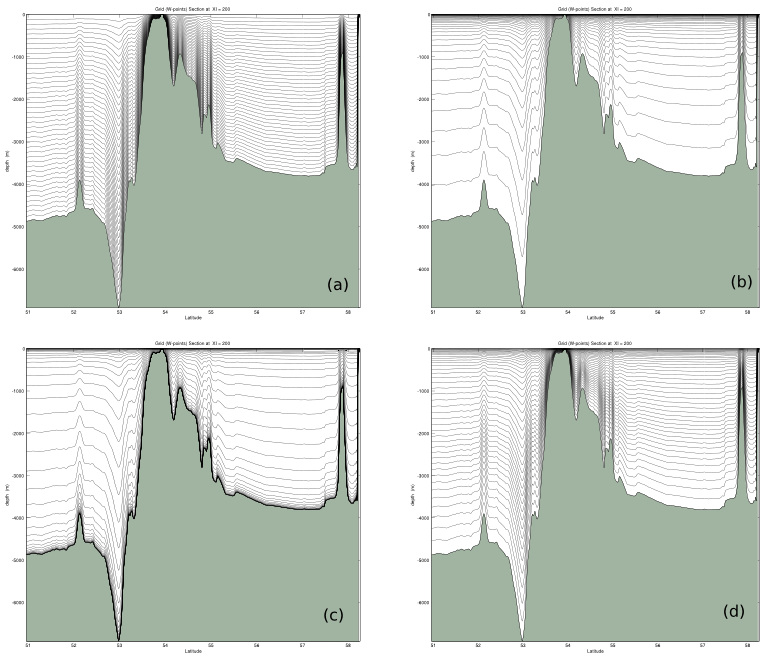
\includegraphics{pics/scoord}
\end{picture}

\caption{The $\sigma$-surfaces for the North Atlantic with (a) $\theta =
0.0001$ and $b = 0$, (b) $\theta = 8$ and $b = 0$, (c) $\theta = 8$
and $b = 1$.  (d) The actual values used in this domain were
$\theta = 5$ and $b = 0.4$.}
\label{fscd}
\end{figure}

We find it convenient to define:
\begin{equation}
   H_z \equiv {\partial z \over \partial \sigma} = (\zeta + h) +
   (h - h_c) {\partial C(\sigma) \over \partial \sigma} .
\end{equation}
The derivative of $C(\sigma)$ can be computed analytically:
\begin{equation}
   {\partial C(\sigma) \over \partial \sigma} = (1-b) {\cosh (\theta
   \sigma) \over
   \sinh \theta} \theta + b {\coth ( {1 \over 2} \theta) \over
   2 \cosh^2 [ \theta (\sigma + {1\over 2})] } \theta .
\end{equation}
However, we choose to compute $H_z$ discretely as $\Delta z/ \Delta
\sigma$ since this leads to the vertical sum of $H_z$ being exactly the
total water depth $D$.

Note that though we have used this form of $\sigma$-coordinate, ROMS
is written in such a way as to work with a variety of vertical
mappings. There is one feature which is critical, however. If the free
surface is at rest, $\zeta = 0$, you get one solution for the level
depths $z^{(0)}(k)$. In the case of nonzero $\zeta$, the
displacements must be proportional to $\zeta$ and to the original
distance from the bottom:
\begin{equation}
   z(k) =  z^{(0)} (k) + \zeta \left( 1 + {z^{(0)} (k) \over h}
   \right)
\end{equation}
or
\begin{equation}
   \Delta z(k) = \Delta z^{(0)} (k) \left( 1 + {\zeta \over h}
   \right)
\end{equation}
This ensures that the vertical mass fluxes generated by a purely
barotropic motion will vanish at every interface.

\section{Horizontal curvilinear coordinates}
\label{Curve}
The requirement for a boundary-following coordinate system and for a
laterally variable grid resolution can both be met (for suitably
smooth domains) by introducing an appropriate orthogonal coordinate
transformation in the horizontal.  Let the new coordinates be
$\xi(x,y)$ and $\eta(x,y)$ where the relationship of horizontal arc
length to the differential distance is given by:
\begin{equation}
   (ds)_{\xi} = \left( {1 \over m} \right) d \xi
\end{equation}
\begin{equation}
   (ds)_{\eta} = \left( {1 \over n} \right) d \eta
\end{equation}
Here, $m(\xi,\eta)$ and $n(\xi,\eta)$ are the scale factors which
relate the differential distances $(\Delta \xi,\Delta \eta)$ to the
actual (physical) arc lengths.

It is helpful to write the equations in vector notation and to use
the formulas for div, grad, and curl in curvilinear coordinates (see
Batchelor, Appendix 2, \cite{Batchelor}):
\begin{equation}
   \nabla \phi = \hat{\xi} m {\partial \phi \over \partial \xi} +
                 \hat{\eta} n {\partial \phi \over \partial \eta}
\end{equation}
\begin{equation}
   \nabla \cdot \vec{a} = mn \left[
   {\partial \over \partial \xi} \!\! \left( {a \over n} \right) +
   {\partial \over \partial \eta} \!\! \left( {b \over m} \right)
   \right]
\end{equation}
\begin{equation}
   \nabla \times \vec{a} = mn \left| \begin{array}{ccc}
   \vspace{1 mm}
   {\hat{\xi}_1 \over m} & {\hat{\xi}_2 \over n} & \hat{k} \\
   \vspace{1 mm}
   {\partial \over \partial \xi} &
   {\partial \over \partial \eta} &
   {\partial \over \partial z} \\
   {a \over m} & {b \over n} & c
   \end{array} \right|
\end{equation}
\begin{equation}
   \nabla^2 \phi = \nabla \cdot \nabla \phi = mn \left[ 
   {\partial \over \partial \xi} \!\! \left( {m \over n} 
   {\partial \phi \over \partial \xi} \right) +
   {\partial \over \partial \eta} \!\! \left( {n \over m} 
   {\partial \phi \over \partial \eta} \right) \right]
\end{equation}
where $\phi$ is a scalar and $\vec{a}$ is a vector with components
$a$, $b$, and $c$.

\section{Viscosity and Diffusion}
\label{Nu}

\subsection{Horizontal viscosity}
The horizontal viscosity and diffusion coefficients are scalars which
are read in from \code{ocean.in}.  Several
factors to consider when choosing these values are:
\begin{klist}
   \kitem{spindown time}  The spindown time on wavenumber $k$ is ${1
   \over k^2 \nu_2}$ for the Laplacian operator and ${1 \over k^4
   \nu_4}$ for the biharmonic operator.  The smallest wavenumber
   corresponds to the length $2 \Delta x$ and is $k = {\pi \over
   \Delta x}$, leading to
\begin{equation}
    \Delta t < t_{damp} = {\Delta x^2 \over \pi^2 \nu_2}
    \mbox{\quad or \quad} {\Delta x^4 \over \pi^4 \nu_4}
\end{equation}
This time should be short enough to damp out the numerical noise
which is being generated but long enough on the larger scales to
retain the features you are interested in.  This time should also be
resolved by the model timestep.
   \kitem{boundary layer thickness} The western boundary layer has a
   thickness proportional to 
\begin{equation}
    \Delta x < L_{BL} = \left( {\nu_2 \over \beta} \right)^{1 \over 3}
    \mbox{\quad and \quad}
    \left( {\nu_4 \over \beta} \right)^{1 \over 5}
\end{equation}
for the Laplacian and biharmonic viscosity, respectively.  We have
found that the model typically requires the boundary layer to be
resolved with at least one grid cell.  This leads to coarse grids
requiring large values of $\nu$.
\end{klist}

\subsection{Horizontal Diffusion}
We have chosen anything from zero to the value of the horizontal
viscosity for the horizontal diffusion coefficient.  One common choice
is an order of magnitude smaller than the viscosity.

\subsection{Vertical Viscosity and Diffusion}
ROMS stores the vertical mixing coefficients in arrays with three
spatial dimensions called
\code{Akv} and \code{Akt}.  \code{Akt} also has a fourth dimension
specifying which tracer, so
that temperature and salt can have differing values.  Both \code{Akt}
and \code{Akv} are stored at $w$-points in the model;
horizontal averaging is done to obtain \code{Akv} at the horizontal $u$
and $v$-points.  The values for these coefficients can be set in a
number of ways, as described in \S\ref{Vmix}.

\section{Radiant heat fluxes}
\label{shortwave}

As was seen in \S\ref{Growth}, the model thermodynamics requires
fluxes of latent and sensible heat and longwave and shortwave
radiation.  We follow the lead of
\citet{Parkinson} in computing these terms.

\subsection{Shortwave radiation}

The Zillman equation for radiation under cloudless skies is:
\begin{equation}
   Q_o = {S \cos^2 Z \over (\cos Z + 2.7) e \times 10^{-5} + 1.085
   \cos Z + 0.10}
\end{equation}
where the variables are as in Table \ref{radvars}.  The cosine of the
zenith angle is computed using the formula:
\begin{equation}
   \cos Z = \sin \phi \sin \delta + \cos \phi \cos \delta \cos H\!A .
\end{equation}
The declination is 
\begin{equation}
   \delta = 23.44^{\circ} \times \cos \left[ (172 - {\rm day \, of \, year})
   \times 2 \pi / 365 \right]
\end{equation}
and the hour angle is
\begin{equation}
   H\!A = (12 \, {\rm hours - solar \, time}) \times \pi / 12 .
\end{equation}
The correction for cloudiness is given by
\begin{equation}
   SW\!\!\downarrow = Q_o ( 1 - 0.6 c^3) .
\end{equation}
%An estimate of the cloud fraction $c$ will be provided by Jennifer
%Francis \citep{Francis00}.

\begin{table}[t]
\hspace{11 mm}
\vbox{
\begin{tabular}{|c|c|l|} \hline
Variable & Value & Description \\ \hline

$(a,b)$ & (9.5, 7.66) & vapor pressure constants over ice \\
$(a,b)$ & (7.5, 35.86) & vapor pressure constants over water \\
$c$ && cloud cover fraction \\
$C_E$ & $1.75 \times 10^{-3}$ & transfer coefficient for latent heat \\
$C_H$ & $1.75 \times 10^{-3}$ & transfer coefficient for sensible heat\\
$c_p$ & 1004 J kg$^{-1}$ K$^{-1}$ & specific heat of dry air \\
$\delta$ && declination \\
$e$ && vapor pressure in pascals \\
$e_s$ && saturation vapor pressure \\
$\epsilon$ & 0.622 & ratio of molecular weight of water to dry air \\
$H\!A$ && hour angle \\
$L$ & $2.5 \times 10^6$ J kg$^{-1}$ & latent heat of vaporization \\
$L$ & $2.834 \times 10^6$ J kg$^{-1}$ & latent heat of sublimation \\
$\phi$ && latitude \\
$Q_o$ && incoming radiation for cloudless skies \\
$q_s$ && surface specific humidity \\
$q_{10 \rm m}$ && 10 meter specific humidity \\
$\rho_a$ && air density \\
$S$ & 1353 W m$^{-2}$ & solar constant \\
$\sigma$ & $5.67 \times 10^{-8}$ W m$^{-2}$ K$^{-4}$ &
Stefan-Boltzmann constant \\
$T_a$ && air temperature \\
$T_d$ && dew point temperature \\
$T_{s\!f\!c}$ && surface temperature of the water/ice/snow \\
$V_{wg}$ && geostrophic wind speed \\
$Z$ && solar zenith angle \\

\hline
\end{tabular}
}
\caption{Variables used in computing the incoming radiation and latent
and sensible heat}
\label{radvars}
\end{table}

\subsection{Longwave radiation}

The clear sky formula for incoming longwave radiation is given by:
\begin{equation}
   F\!\downarrow\, = \sigma T_a^4 \left\{1 - 0.261 \exp \left[ -7.77 \times 10^{-4}
   (273 - T_a) ^2 \right] \right\}
\end{equation}
while the cloud correction is given by:
\begin{equation}
   LW\!\downarrow\, = (1 + 0.275 c)\, F\!\downarrow .
\end{equation}

\subsection{Sensible heat}

The sensible heat is given by the standard aerodynamic formula:
\begin{equation}
   H\!\downarrow\, = \rho_a c_p C_H V_{wg} (T_a - T_{s\!f\!c}) .
\end{equation}

\subsection{Latent heat}

The latent heat depends on the vapor pressure and the saturation vapor
pressure given by:
\begin{eqnarray}
   e & = & 611 \times 10^{a(T_d - 273.16) / (T_d - b)} \\
   e_s & = & 611 \times 10^{a(T_{s\!f\!c} - 273.16) / (T_{s\!f\!c} - b)}
\end{eqnarray}
The vapor pressures are used to compute specific humidities according
to:
\begin{eqnarray}
   q_{10 \rm m} & = & {\epsilon e \over p - (1 - \epsilon) e} \\
   q_s & = & {\epsilon e_s \over p - (1 - \epsilon) e_s}
\end{eqnarray}
The latent heat is also given by a standard aerodynamic formula:
\begin{equation}
   LE\!\downarrow\, = \rho_a L C_E V_{wg} (q_{10 \rm m} - q_s) .
\end{equation}
Note that these need to be computed independently for the ice-covered
and ice-free portions of each gridbox since the empirical factors
$a$ and $b$ and the factor $L$ differ depending on the surface type.

\section{The C preprocessor}
\label{Cpp}

The C preprocessor, \code{cpp}, is a standalone program which comes
with most C compilers.  On many UNIX systems it is not in the default
path, but in \code{/lib} or in \code{/usr/lib}.  If you do not have a C
preprocessor then there are several versions available via anonymous
ftp.  For instance, \code{ftp.uu.net} has two in the
\code{/published/oreilly/nutshell/imake} directory---I have built and
used the one from Der Mouse on a Cray.  I have put this one in
pub/util/cpp.tar.gz on the ahab.rutgers.edu ftp site since it supports
the \code{\#elif} construct.  One also comes with \code{gcc},
the \code{gnu} C compiler.  If you build this compiler, \code{cpp} will
have a path such as

\begin{verbatim}
       /usr/local/lib/gcc-lib/sparc-sun-solaris2.5/2.7.2/cpp
\end{verbatim}
where \code{sparc} is the architecture, \code{sun} is  the
manufacturer, \code{solaris2.5} is the operating system and version,
and \code{2.7.2} is \code{gcc}'s version number.

This Appendix describes the C preprocessor as used in SCRUM with the
Fortran language.  A more complete description is given by
Kernighan and Ritchie \cite{K&R}.  More practical advice on using
\code{cpp} is given by Hazard \cite{Hazard}.

\subsection{File inclusion}
Placing common blocks in smaller files, which are then included in each
subroutine, is the easiest way to make sure that the common blocks are
declared consistently.  Many Fortran compilers support an include
statement where the compiler replaces the line
\begin{verbatim}
            include 'file.h'
\end{verbatim}
with the contents of \code{file.h}; \code{file.h} is assumed
to be in the current directory.  The C preprocessor has an equivalent
include statement:
\begin{verbatim}
      #include "file.h"
\end{verbatim}
We are using the C preprocessor style of include because many of the
SCRUM include files are not pure Fortran and must be processed by
\code{cpp}.

\subsection{Macro substitution}
A macro definition has the form
\begin{verbatim}
      #define    name           replacement text
\end{verbatim}
where \code{name} would be replaced with ``replacement text''
throughout the rest of the file.  This is used in SCRUM as a
reasonably portable way to get 64-bit precision:
\begin{verbatim}
      #define  BIGREAL     real*8
\end{verbatim}
It is customary to use uppercase for \code{cpp} macros---the C
preprocessor is case sensitive.

It is also possible to define macros with arguments, as in
\begin{verbatim}
      #define av2(a1,a2)        (.5 * ((a1) + (a2)))
\end{verbatim}
although this is riskier than the equivalent statement function
\begin{verbatim}
            av2(a1,a2) = .5 * (a1 + a2)
\end{verbatim}
The statement function is preferable because it allows the compiler
to do type checking and because you don't have to be as careful
about using enough parentheses.

The third form of macro has no replacement text at all:
\begin{verbatim}
      #define  MASKING
\end{verbatim}
In this case, \code{MASKING} will evaluate to \code{true} in the
conditional tests described below.

\subsection{Conditional inclusion}
It is possible to control which parts of the code are seen by the
Fortran compiler by the use of \code{cpp}'s conditional inclusion.
For example, the statements
\begin{verbatim}
      #ifdef MASKING
      # include "mask.h"
      #endif /* MASKING */
              :
      # ifdef MASKING
      c
      c  Apply Land/Sea mask: slipperiness.
      c
            do j=1,M
              do i=2,Lm
                Uflux(i,j)=Uflux(i,j)*pmask(i,j)
              enddo
            enddo
      # endif /* MASKING */
\end{verbatim}
will not be in the Fortran source code if \code{MASKING} has not
been defined.  Likewise,
\code{\#ifndef} tests for a macro being undefined:
\begin{verbatim}
      #ifndef RMDOCINC
      c  rmask       Mask at RHO-points (0=Land, 1=Sea).
      c  pmask       Slipperiness mask at PSI-points (0=Land, 1=Sea,
      c                                               1-gamma2=boundary).
      c  umask       Mask at U-points (0=Land, 1=Sea).
      c  vmask       Mask at V-points (0=Land, 1=Sea).
      c
      c=======================================================================
      #endif
\end{verbatim}

There are also \code{\#else} and \code{\#elif} (else if) statements,
although \code{\#elif} is newer and is not supported by all versions of
\code{cpp}.  An example using \code{\#else} and \code{\#elif} is
shown:
\begin{verbatim}
#ifdef SOLITON
        real(r8) :: g = 1.0_r8                  ! non-dimensional
# elif defined WBC_1 || defined WBC_2 || defined WBC_3
        real(r8) :: g = 9.8_r8                  ! m/s2
# elif defined CIRCLE
        real(r8) :: g = 3.92e-2_r8                  ! m/s2
#else
        real(r8) :: g = 9.81_r8                 ! m/s2
#endif
\end{verbatim}

Actually, \code{\#ifdef} is a restricted version of the more general
test
\begin{verbatim}
      #if     expression
\end{verbatim}
where ``expression'' is a constant integer value.  Zero evaluates
to \code{false} and everything else is considered \code{true}.
Compound expressions may be built using the C logical operators:
\begin{verbatim}
        &&           logical and
        ||           logical or
        !            logical not
\end{verbatim}
These symbols would be used as in the following example:
\begin{verbatim}
      #if defined CANYON_A || defined CANYON_B
            do j=0,M
              do i=0,L
                yc=c32000-c16000*(sin(pi*xr(i,j)/xl))**24
                h(i,j)=c20+p5*(hmax-c20)*(c1+tanh((yr(i,j)-yc)/c10000))
              enddo
            enddo
      #endif
\end{verbatim}

\subsection{C comments}
The C preprocessor will also delete C language comments starting
with \code{/*} and ending with \code{*/} as in:
\begin{verbatim}
       #endif  /* MASKING */
\end{verbatim}
When mixed with Fortran code, it is safer to use a Fortran
comment.

\subsection{Potential problems}
The use of the C preprocessor is not entirely free of problems, but
many can be worked around or avoided by using the Der Mouse version of
\code{cpp}.
   \begin{enumerate}
     \item Apostrophes in Fortran comments.  \code{cpp} does not
     know that it is in a comment and some versions will complain about
     unmatched apostrophes in the following:
     \begin{verbatim}
  c  Some useful comment about Green's functions.
     \end{verbatim}
     The \code{gnu} version of \code{cpp} (which comes with \code{gcc})
     has a \code{-traditional} option which makes it more
     appropriate for use with Fortran.
     \item \CC\ comments.  Some of the newer versions of
     \code{cpp} will remove \CC\ comments which go from '//' to
     the end of the line.  Some perfectly reasonable Fortran lines
     contain two consecutive slashes, such as:
     \begin{verbatim}
        common // var1, var2
    44  format(//)
     \end{verbatim}
     and the new Fortran 90 string concatenation:
     \begin{verbatim}
        mystring = 'Hello, ' // 'World!'
     \end{verbatim}
     \item Macro replacement.  One feature of \code{cpp} is that you
     can define macros and have it perform replacements.  The code:
     \begin{verbatim}
  #define REAL double precision
        REAL really_long_variable, second_long_variable
     \end{verbatim}
     becomes
     \begin{verbatim}
        double precision really_long_variable, second_long_variable
     \end{verbatim}
     and you run the risk of creating lines which are longer than 72
     characters in length.

     Also, make sure that your macros will not be found anywhere else
     in the code.  I used to use \code{\#define DOUBLE} for double
     precision until it was pointed out to me that \code{DOUBLE 
     PRECISION} is perfectly valid Fortran.  The macro processor would
     turn this into \code{1 PRECISION} since something that is defined
     has a value of 1.
  \end{enumerate}

\subsection{Modern Fortran}
I started working on these ocean models before 1990, much less before
Fortran 90 compilers were generally available.  Fortran 90's
\code{kind} feature would be a better way to handle the \code{BIGREAL}
type declarations.  On the other hand, Fortran 90 does not include
conditional compilation.  However, it is deemed useful enough that the
Fortran 2000 committee has a draft document describing how Fortran
might support conditional compilation.  We {\em might} start using this
in about ten years.

%\section{The \code{patch} program}
\label{Patch}
We sometimes discover things in SCRUM which we would like to modify,
either to fix bugs, or to add new features.
Hernan Arango keeps track of these changes
and periodically sends patches to the
list of known SCRUM users so that they can update their versions.  By
sending out these changes rather than the whole updated model, people
can acquire bug fixes and still retain the changes they have made to
SCRUM for their own applications.

Larry Wall has written a program to take the output of \code{diff} and
automatically apply it to the old version of a file to create the new
version.  This program is called \code{patch} and is available from all
the \code{gnu} archive sites.  If the output of \code{diff} has been
saved in the file \code{scrum.patch.20} then \code{patch} would be used
as follows:
\begin{verbatim}
        patch < scrum.patch.20
\end{verbatim}
As \code{patch} updates the files, it leaves the original of
\code{file} in \code{file.orig}.  If it gets confused for some reason
(if you modified the lines of code \code{patch} wants to change)
it will create a \code{file.rej} file.  I
often check to see if any \code{.rej} files get created---these can be
used to patch \code{file} by hand and can then be deleted.

%\newpage
%\mbox{}
\section{\code{Makefiles}}
\label{Gmake}
One of the software development tools which comes with the UNIX
operating system is called \code{make}. \code{Make} has many uses,
but is most commonly used to keep track of how a large program
should be compiled. ROMS now requires the \code{gnu} version of 
\code{make}, sometimes known as \code{gmake} (Mecklenburg \cite{GMAKE}).
This appendix describes generic \code{make}, the \code{gnu}
enhancements to \code{make}, as well as describing the
\code{makefile} structure used in ROMS. This material first
appeared in the \href{http://www.arsc.edu/support/news/HPCnews.shtml}{ARSC
HPC Newsletter} in several segments and has been updated and restructured
here.

\subsection{Introduction to Portable \code{make}}

\code{Make} gets its instructions from a description file, by default named
\code{makefile} or \code{Makefile}. This file is called the
\code{Makefile}, but other files
can be used by invoking \code{make} with the \code{-f} option:
\begin{verbatim}
     make -f Makefile.yukon
\end{verbatim}

The ancester to ROMS originally had a \code{Makefile} that looked
something like:
\begin{verbatim}
model: main.o init.o plot.o
<TAB>   f77 -o model main.o init.o plot.o

main.o: main.f
<TAB>   f77 -c -O main.f

init.o: init.f
<TAB>   f77 -c -O init.f

plot.o: plot.f
<TAB>   f77 -c -O0 plot.f

clean:
<TAB>   rm *.o core
\end{verbatim}
The default thing to build is \code{model}, the first target. The syntax
is:
\begin{verbatim}
target: dependencies
<TAB>  command
<TAB>  command
\end{verbatim}
The target \code{model} depends on the object files, \code{main.o}
and friends. They have to exist and be up to date before model's link
command can be run. If the target is out of date according to the
timestamp on the file, then the commands will
be run. Note that the tab is required on the command lines.

The other targets tell \code{make} how to create the object files
and that they in turn have dependencies.  To compile \code{model}, simply
type ``\code{make}''. \code{Make} will look for the file \code{makefile},
read it, and do whatever is necessary to make \code{model} up
to date. If you edit \code{init.f}, that file will be newer than
\code{init.o}. \code{Make} would see that \code{init.o} is out of date
and run the ``\code{f77 -c -O init.f}'' command. Now \code{init.o}
is newer than \code{model}, so the link command ``\code{f77 -o model
main.o init.o plot.o}'' must be executed.

To clean up, type ``\code{make clean}'' and the \code{clean} target will
be brought up to date. The \code{clean} target has no dependencies. What
happens in that case is that the command (``\code{rm *.o core}'') will
always be executed.

The original version of this \code{Makefile} turned off
optimization on \code{plot.f} due to a compiler bug, but hopefully you
won't ever have to worry about that.

\subsubsection{Macros}

\code{Make} supports a simple string substitution macro. Set it with:
\begin{verbatim}
MY_MACRO = nothing today
\end{verbatim}
and refer to it with:
\begin{verbatim}
$(MY_MACRO)
\end{verbatim}

The convention is to put the macros near the top of your \code{Makefile}
and to use upper case. Also, use separate macros for the name of
your compiler and the flags it needs:
\begin{verbatim}
F90 = f90
F90FLAGS = -O3
LIBDIR = /usr/local/lib
LIBS = -L$(LIBDIR) -lmylib
\end{verbatim}

Let's rewrite our \code{Makefile} using macros:
\begin{verbatim}
#
# IBM version
#
F90 = xlf90_r
F90FLAGS = -O3 -qstrict
LDFLAGS = -bmaxdata:0x40000000

model: main.o init.o plot.o
        $(F90) $(LDFLAGS) -o model main.o init.o plot.o

main.o: main.f
        $(F90) -c $(F90FLAGS) main.f

init.o: init.f
        $(F90) -c $(F90FLAGS) init.f

plot.o: plot.f
        $(F90) -c $(F90FLAGS) plot.f

clean:
        rm *.o core
\end{verbatim}

Now when we change computers, we only have to change the compiler name
in one place. Likewise, if we want to try a different optimization level,
we only specify that in one place.

Notice that you can use comments by starting the line with a \code{\#}.

\subsubsection{Implicit Rules}

\code{Make} has some rules already built in. For fortran, you might be able
to get away with:
\begin{verbatim}
OBJS = main.o init.o plot.o

model: $(OBJS)
        $(FC) $(LDFLAGS) -o model $(OBJS)
\end{verbatim}
as your whole \code{Makefile}. \code{Make} will automatically invoke its
default Fortran compiler, possibly \code{f77} or \code{g77}, with whatever
default compile options it happens to have (\code{FFLAGS}). One built
in rule often looks like:
\begin{verbatim}
.c.o:
        $(CC) $(CFLAGS) -c $<
\end{verbatim}
which says to compile \code{.c} files to \code{.o} files using the
compiler \code{CC} and options \code{CFLAGS}. We can write our own suffix
rules in this same style.  The only thing to watch for is that make by
default has a limited set of file extentions that it knows about. Let's
write our \code{Makefile} using a suffix rule:
\begin{verbatim}
#
# Cray version
#
F90 = f90
F90FLAGS = -O3
LDFLAGS =

.f.o:
        $(F90) $(F90FLAGS) -c $<

model: main.o init.o plot.o
        $(F90) $(LDFLAGS) -o model main.o init.o plot.o

clean:
        rm *.o core
\end{verbatim}

\subsubsection{Dependencies}

There may be additional dependencies beyond the \code{source->object} ones.
In our little example, all our source files include a file called
\code{commons.h}. If \code{commons.h} gets modified to add a new variable,
everything must be recompiled. \code{Make} won't know that unless you
tell it:
\begin{verbatim}
# include dependencies
main.o: commons.h
init.o: commons.h
plot.o: commons.h
\end{verbatim}
Fortran 90 introduces module dependencies as well. See \S\ref{sfm}
for how we automatically generate this dependency information.

The most common newbie mistake is to forget that the commands after
a target {\em have} to start with a tab.

\subsection{\code{gnu make}}

Over the years, the community has moved from the stance of writing
portable \code{Makefiles} to a stance of just using a powerful, portable
\code{make}. The previous section described a portable subset of
\code{make} features. We now delve into some of the more powerful
tools available in \code{gnu make}.

\subsubsection{Make rules}

The core of \code{make} hasn't changed in decades, but concentrating on
\code{gmake} allows one to make use of its nifty little extras designed
by real programmers to help with real projects. The first change that
matters to my \code{Makefiles} is the change from suffix rules to
pattern rules. I've always found the \code{.SUFFIXES} list to be odd,
especially since \code{.f90} is not in the default list. Good riddance
to all of that! For a concrete example, the old way to provide a rule
for going from \code{file.f90} to \code{file.o} is:
\begin{verbatim}
.SUFFIXES: .o .f90 .F .F90
.f90.o:
<TAB>   $(FC) -c $(FFLAGS) $<
\end{verbatim}
while the new way is:
\begin{verbatim}
%.o: %.f90
<TAB>   $(FC) -c $(FFLAGS) $<
\end{verbatim}
In fact, going to a uniform \code{make} means that we can figure out what
symbols are defined and use their standard values---in this case,
\$\code{(FC)} and \$\code{(FFLAGS)} are the built-in default names
for the compiler and its options.
If you have any
questions about this, you can always run \code{make} with the \code{-p} (or
\code{-\mbox{}-print-data-base}) option. This prints out all the rules
\code{make} knows about, such as:
\begin{verbatim}
# default
COMPILE.f = $(FC) $(FFLAGS) $(TARGET_ARCH) -c
\end{verbatim}
Printing the rules database will show variables that \code{make} is
picking up from the environment, from the \code{Makefile}, and from its
built-in rules---and which of these sources is providing each
value.

\subsubsection{Assignments}

In the old days, I only used one kind of assignment: \code{=} (equals
sign). \code{Gmake} has several kinds of assignment (other \code{makes}
might as well, but I no longer have to know or care). An example of
the power of \code{gnu make} is shown by an example from my Cray X1
\code{Makefile}.  There is a routine which runs much more quickly if a
short function in another file is inlined. The way to accomplish this is
through the \code{-O inlinefrom=file} directive to the compiler. I can't
add this option to \code{FFLAGS}, since the inlined routine won't compile
with this directive---there is only the one file that needs it. I had:
\begin{verbatim}
    FFLAGS = -O 3,aggress -e I -e m
    FFLAGS2 = -O 3,aggress -O inlinefrom=lmd_wscale.f90 -e I -e m

lmd_skpp.o:
<TAB>   $(FC) -c $(FFLAGS2) $*.f90
\end{verbatim}
The first change I can make to this using other assignments is:
\begin{verbatim}
    FFLAGS := -O 3,aggress -e I -e m
    FFLAGS2 := $(FFLAGS) -O inlinefrom=lmd_wscale.f90
\end{verbatim}
The \code{:=} assignment means to evaluate the right hand side immediately.
In this case, there is no reason not to, as long as the second
assigment follows the first one (since it's using the value of
\$\code{(FFLAGS))}. For the plain equals, \code{make} doesn't evaluate the
right-hand side until its second pass through the \code{Makefile}. However,
\code{gnu make}
supports an assignment which avoids the need for \code{FFLAGS2} entirely:
\begin{verbatim}
lmd_skpp.o: FFLAGS += -O inlinefrom=lmd_wscale.f90
\end{verbatim}
What this means is that for the target \code{lmd\_skpp.o} only, append the
inlining directive to \code{FFLAGS}. I think this is pretty cool!

One last kind of assignment is to set the value only if there is no
value from somewhere else (the environment, for instance):
\begin{verbatim}
     FC ?= mpxlf90_r
\end{verbatim}
If we used \code{:=} or \code{=}, we would override the value from the
environment.

\subsubsection{Include and a Few Functions}
\label{Inc_fort}

One reasonably portable \code{make} feature is the include directive. It
can be used to clean up the \code{Makefile} by putting bits in an
include file. The syntax is simply:
\begin{verbatim}
   include file
\end{verbatim}
and we use it liberally to keep the project
information neat. We can also include a file with the system/compiler
information in it, assuming we have some way of deciding {\em which}
file to include. We can use \code{uname -s} to find out which operating
system we're using. We also need to know which compiler we're using.

One user-defined variable is called \code{FORT}, the name of the
Fortran compiler. This value is combined with the result of
``\code{uname -s}'' to
provide a machine and compiler combination. For instance, \code{ftn} on
Linux is the Cray cross-compiler. This would link to a different copy
of the NetCDF library and use different compiler flags than the Intel
compiler which might be on the same system.
\begin{verbatim}
# The user sets FORT:
  FORT ?= ftn
  OS := $(shell uname -s | sed 's/[\/ ]/-/g')

  include $(COMPILERS)/$(OS)-$(strip $(FORT)).mk
\end{verbatim}
We pick one include file at compile time, here picking
\code{Linux-ftn.mk}, containing the Cray cross-compiler information. The
value \code{Linux} comes from the \code{uname} command, the \code{ftn}
comes from the user, and the two are concatenated.
The sed command will turn the
slash in \code{UNICOS/mp} into a dash; the native Cray include file is
\code{UNICOS-mp-ftn.mk}. Strip is a built-in function to strip away
any extra white space.

Another tricky system is \code{CYGWIN}, which puts a version number
in the \code{uname} output, such as \code{CYGWIN\_NT-5.1}. \code{Gnu make} has
quite a few built-in functions, one of which allows us to do string
substitution:
\begin{verbatim}
OS := $(patsubst CYGWIN_%,CYGWIN,$(OS))
\end{verbatim}
In \code{make}, the \code{\%} symbol is a sort of wild card, much
like \code{*} in the shell.
Here, we match \code{CYGWIN} followed by an underscore and anything else,
replacing the whole with simply \code{CYGWIN}. Another example of a
built-in function is the substitution we do in:
\begin{verbatim}
   objects = $(subst .F,.o,$(sources))
\end{verbatim}
where we build our list of objects from the list of sources.
There are quite a few other functions, plus the user can define
their own. From the book\cite{GMAKE}:
\begin{quote}
GNU make supports both built-in and user-defined functions.
A function invocation looks much like a variable reference, but
includes one or more parameters separated by commas.  Most built-in
functions expand to some value that is then assigned to a variable
or passed to a subshell. A user-defined function is stored in a
variable or macro and expects one or more parameters to be passed
by the caller.
\end{quote}
We will show some user-defined functions in \S\ref{make_fun2}.

\subsubsection{Conditionals}

We used to have way too many \code{Makefiles}, a separate one for each
of the serial/MPI/OpenMP versions on each system (if supported). For
instance, the name of the IBM compiler changes when using MPI; the
options change for OpenMP. The compiler options also change when using
64-bit addressing or for debugging.
A better way to organize this is to have the user select 64-bit or not, MPI
or not, etc., then use conditionals. The complete list of
user definable \code{make} variables is given in \S\ref{make_var}.

\code{Gnu make} supports two kinds of \code{if} test, \code{ifdef} and
\code{ifeq} (plus the
negative versions \code{ifndef, ifneq}). The example from the book is:
\begin{verbatim}
ifdef COMSPEC
   # We are running Windows
else
   # We are not on Windows
endif
\end{verbatim}
An example from the IBM include file is:
\begin{verbatim}
ifdef USE_DEBUG
           FFLAGS += -g -qfullpath
else
           FFLAGS += -O3 -qstrict
endif
\end{verbatim}
To test for equality, an example is:
\begin{verbatim}
ifeq ($(USE_MPI),on)
   # Do MPI things
endif
\end{verbatim}
or 
\begin{verbatim}
ifeq "$(USE_MPI)" "on"
   # Do MPI things
endif
\end{verbatim}
The user has to set values for the \code{USE\_MPI}, \code{USE\_DEBUG},
and \code{USE\_LARGE} switches in the \code{Makefile} or the build
script {\em before} the compiler-dependent piece is included:
\begin{verbatim}
    USE_MPI ?= on
    USE_DEBUG ?=
    USE_LARGE ?=
\end{verbatim}
The \code{Makefile} uses the conditional assign ``\code{?=}''
in case a build script is used to set them in the environment.
Be sure to leave the switches meant to be off set to an empty string---the
string ``\code{off}'' will test true on an \code{ifdef} test.

\subsection{Multiple Source Directories the ROMS Way}

There's more than one way to divide your sources into separate
directories. The choices we have made include nonrecursive \code{make}
and putting the temporary files in their own \code{\$(SCRATCH\_DIR)}
directory. These include the \code{.f90} files which have been through
the C preprocessor, object files, module files, and libraries.

\subsubsection{Directory Structure}

The directory structure of the source code has the top directory,
a \code{Master} directory, a \code{ROMS} directory with a number of
subdirectories, and several other directories. \code{Master} contains
the main program while the rest contain sources for libraries and
other files. Note that the bulk of the source code gets compiled into
files that become libraries with the \code{ar} command, one library per
directory. There is also a \code{Compilers} directory for the system-
and compiler-specific \code{Makefile} components.

\subsubsection{Conditionally Including Components}

The \code{makefile} will build the lists of libraries to create and source
files to compile. They start out empty at the top of the
\code{makefile}:
\begin{verbatim}
  sources    := 
  libraries  :=
\end{verbatim}
That's simple enough, but the list of directories to search for
these sources will depend on the options chosen by the user, not
just in the \code{make} options (\S\ref{make_var}), but inside the
\code{ROMS\_HEADER} file as well. How does this happen? Once \code{make}
knows how to find the \code{ROMS\_HEADER}, it is used by \code{cpp}
to generate an include file telling \code{make} about these other options.
\begin{verbatim}
MAKE_MACROS := Compilers/make_macros.mk
 MACROS := $(shell cpp -P $(ROMS_CPPFLAGS) Compilers/make_macros.h > \
                 $(MAKE_MACROS); $(CLEAN) $(MAKE_MACROS))
\end{verbatim}
The \code{make\_macros.h} file contains blocks such as:
\begin{verbatim}
#ifdef SWAN_COUPLING
  USE_SWAN := on
#else
  USE_SWAN :=
#endif
\end{verbatim}
The resulting \code{make\_macros.mk} file will simply end up with
either 
\begin{verbatim}
  USE_SWAN := on
\end{verbatim}
or
\begin{verbatim}
  USE_SWAN :=
\end{verbatim}
This file can then be included by the \code{makefile} and the
variable \code{USE\_SWAN} will have the correct state for this
particular compilation. We can now use it and all the similar flags
to build a list of directories.

We initialize two lists:
\begin{verbatim}
 modules  :=
 includes :=    ROMS/Include
\end{verbatim}
Add the adjoint bits:
\begin{verbatim}
ifdef USE_ADJOINT
 modules  +=    ROMS/Adjoint
endif
ifdef USE_ADJOINT
 includes +=    ROMS/Adjoint
endif
\end{verbatim}
Add the bits we'll always need:
\begin{verbatim}
 modules  +=    ROMS/Nonlinear \
                ROMS/Functionals \
                ROMS/Utility \
                ROMS/Modules
 includes +=    ROMS/Nonlinear \
                ROMS/Utility \
                ROMS/Drivers
\end{verbatim}
Then we add in some more:
\begin{verbatim}
ifdef USE_SWAN
 modules  +=    Waves/SWAN/Src
 includes +=    Waves/SWAN/Src
endif

 modules  +=    Master
 includes +=    Master Compilers
\end{verbatim}
Now that our lists are complete, let's put them to use:
\begin{verbatim}
vpath %.F $(modules)
vpath %.h $(includes)
vpath %.f90 $(SCRATCH_DIR)
vpath %.o $(SCRATCH_DIR)

include $(addsuffix /Module.mk,$(modules))

CPPFLAGS += $(patsubst %,-I%,$(includes))
\end{verbatim}
\begin{enumerate}
\item \code{vpath} is a standard \code{make} feature for
providing a list of directories for \code{make} to search for files
of different types. Here we are saying that \code{*.F} files can be
found in the directories provided in the \code{\$(modules)} list, and
so on for the others.

\item For each directory in the \code{\$(modules)} list, \code{make}
will include the file \code{Module.mk} that is found there. More on
these later.

\item For each directory in the \code{\$(includes)} list, add
that directory to the list searched by \code{cpp} with the \code{$-$I}
flag.
\end{enumerate}

\subsubsection{User-defined \code{make} Functions}
\label{make_fun2}

The \code{Module.mk} fragments mentioned before call some
user-defined functions.  It's time to show these functions and
talk about how they work. They get defined in the top Makefile:
\begin{verbatim}
#--------------------------------------------------------------------------
#  Make functions for putting the temporary files in $(SCRATCH_DIR)
#--------------------------------------------------------------------------

# $(call source-dir-to-binary-dir, directory-list)
source-dir-to-binary-dir = $(addprefix $(SCRATCH_DIR)/, $(notdir $1))

# $(call source-to-object, source-file-list)
source-to-object = $(call source-dir-to-binary-dir,   \
                   $(subst .F,.o,$(filter %.F,$1)))

# $(call f90-source, source-file-list)
f90-source = $(call source-dir-to-binary-dir,     \
                   $(subst .F,.f90,$1))

# $(call make-library, library-name, source-file-list)
define make-library
   libraries += $(SCRATCH_DIR)/$1
   sources   += $2

   $(SCRATCH_DIR)/$1: $(call source-dir-to-binary-dir,    \
                      $(subst .F,.o,$2))
       $(AR) $(ARFLAGS) $$@ $$^
       $(RANLIB) $$@
endef

# $(call one-compile-rule, binary-file, f90-file, source-files)
define one-compile-rule
  $1: $2 $3
       cd $$(SCRATCH_DIR); $$(FC) -c $$(FFLAGS) $(notdir $2)

  $2: $3
       $$(CPP) $$(CPPFLAGS) $$(MY_CPP_FLAGS) $$< > $$@
       $$(CLEAN) $$@

endef

# $(compile-rules)
define compile-rules
  $(foreach f, $(local_src),       \
    $(call one-compile-rule,$(call source-to-object,$f), \
    $(call f90-source,$f),$f))
endef
\end{verbatim}

\begin{enumerate}

\item We define a function to convert the path from
the source directory to the \code{Build} directory, called
\code{source-dir-to-binary-dir}. Note that the \code{Build} directory
is called \$\code{(SCRATCH\_DIR)} here. All it does is strip off the
leading directory with the the built-in function \code{notdir}, then
paste on the \code{Build} directory.

\item Next comes \code{source-to-object}, which calls the function above to
return the object filename when given the source filename. It assumes
that all sources have a \code{.F} extension.

\item A similar function is \code{f90-source}, which returns the name of the
intermediate source which is created by \code{cpp} from our
\code{.F} file.

\item The \code{Module.mk} fragment in each library source directory invokes
\code{make-library}, which takes the library name and the list of sources
as its arguments. The function adds its \code{library} to the global list
of \code{libraries} and provides rules for building itself. The double
dollar signs are to delay the variable substitution. Note that we call
\code{source-dir-to-binary-dir} instead of \code{source-to-object}---this
is a work-around for a make bug.

\item The next, \code{one-compile-rule}, takes three arguments: the \code{.o}
filename, the \code{.f90} filename, and the \code{.F} filename. From
these, it produces the \code{make} rules for running \code{cpp} and the
compiler.

A note on directories: \code{make} uses \code{vpath} to find the
source file where it resides. It would be possible to compile from
the top directory and put the \code{.o} file in \code{Build} with the
appropriate arguments, but I don't know how to get the \code{.mod} file
into \code{Build} short of a \code{mv} command. Likewise, if we compile
in the top directory, we need to know the compiler option to tell it to
look in \code{Build} for the \code{.mod} files it uses. Doing a \code{cd}
to \code{Build} before compiling is just simpler.

\item The last, \code{compile-rules}, is given a list of sources, then calls
\code{one-compile-rule} once per source file.
\end{enumerate}

Again, you can invoke \code{make -p} to see how \code{make}
internally transforms all this into actual targets and rules.

\subsubsection{Library \code{Module.mk}}

In each library directory, there is a file called \code{Module.mk}
which gets included by the top level \code{makefile}. These
\code{Module.mk} bits build onto the list of sources and libraries
to be compiled and built, respectively.
These \code{Module.mk} files look something like:
\begin{verbatim}
local_sub  := ROMS/Nonlinear
local_lib  := libNLM.a

local_src  := $(wildcard $(local_sub)/*.F)

$(eval $(call make-library,$(local_lib),$(local_src)))

$(eval $(compile-rules))
\end{verbatim}
First, we provide the name of the current directory and the library
to be built from the resident sources.  Next, we use the \code{wildcard}
function to search the subdirectory for these sources. Note that
every \code{.F} file found will be compiled. If you have half-baked
files that you don't want used, make sure they have a different
extension.

Each subdirectory is resetting the \code{local\_src} variable. That's
OK because we're saving the values in the global \code{sources} variable
inside the \code{make-library} function, which also adds the local library
to the \code{libraries} list. The \code{compile-rules} function uses this
\code{local\_src} variable to generate the rules for compiling each file,
placing the resulting files in the \code{Build} directory.

%the user-defined \code{subdirectory} function, from \cite{GMAKE}:
%\begin{verbatim}
%subdirectory  = $(patsubst %/Module.mk,%, \
%                $(word $(words $(MAKEFILE_LIST)),$(MAKEFILE_LIST)))
%\end{verbatim}
%This does the right thing to figure out which subdirectory we are
%in from \code{make}'s internal list of the \code{Makefiles} it is
%parsing. It depends on all the subdirectory include files being called
%\code{Module.mk}.

\subsubsection{Main Program}

The main program is in a directory called \code{Master} and its
\code{Module.mk} is similar to the library one:
\begin{verbatim}
local_sub  := Master
local_src  := $(wildcard $(local_sub)/*.F)

local_objs := $(subst .F,.o,$(local_src))
local_objs := $(addprefix $(SCRATCH_DIR)/, $(notdir $(local_objs)))

sources    += $(local_src)

ifdef LD_WINDOWS
$(BIN): $(libraries) $(local_objs)
        $(LD) $(FFLAGS) $(local_objs) -o $@ $(libraries) $(LIBS_WIN32) $(LDFLAGS)
else
$(BIN): $(libraries) $(local_objs)
        $(LD) $(FFLAGS) $(LDFLAGS) $(local_objs) -o $@ $(libraries) $(LIBS)
endif

$(eval $(compile-rules))
\end{verbatim}
Instead of a rule for building a library, we have a rule for building
a binary \code{\$(BIN)}. In this case, the name of the ROMS binary
is defined elsewhere. The binary depends
on the \code{libraries} getting compiled first, as well as the local
sources. During the link, the \$\code{(libraries)} are compiled from
the sources in the other directories, while \$\code{(LIBS)} are exteral
libraries such as NetCDF.

\subsubsection{Top Level Makefile}

Now we get to the glue that holds it all together. We've covered
many things so far, but there's still a few bits which might be
confusing:
\begin{enumerate}
\item There can be rare cases where you might have special code for
some systems. You can check which system you are on in the \code{.F}
file with:
\begin{verbatim}
#ifdef X86_64
!      special stuff
#endif
\end{verbatim}
To be sure this is defined on each \code{X86\_64} system, it has to
be passed to \code{cpp}:
\begin{verbatim}
CPPFLAGS += -D$(shell echo ${OS} | tr "-" "_" | tr [a-z] [A-Z])
CPPFLAGS += -D$(shell echo ${CPU} | tr "-" "_" | tr [a-z] [A-Z])
CPPFLAGS += -D$(shell echo ${FORT} | tr "-" "_" | tr [a-z] [A-Z])

CPPFLAGS += -D'ROOT_DIR="$(ROOTDIR)"'
ifdef ROMS_APPLICATION
  CPPFLAGS  += $(ROMS_CPPFLAGS)
  CPPFLAGS  += -DNestedGrids=$(NestedGrids)
  MDEPFLAGS += -DROMS_HEADER="$(HEADER)"
endif
\end{verbatim}
This guarantees that \code{CPPFLAGS} will have terms in it such
as:
\begin{verbatim}
       -DLINUX -DX86_64 -DPGI
       -D'ROOT_DIR="/export/staffdata/kate/roms/trunk"' -DSHOREFACE
       -D'HEADER="shoreface.h"' -D'ROMS_HEADER="shoreface.h"'
       -DNestedGrids=1
\end{verbatim}

\item For \code{mod\_strings.F}, there is a special case:
\begin{verbatim}
$(SCRATCH_DIR)/mod_strings.f90: CPPFLAGS += -DMY_OS='"$(OS)"' \
              -DMY_CPU='"$(CPU)"' -DMY_FORT='"$(FORT)"' \
              -DMY_FC='"$(FC)"' -DMY_FFLAGS='"$(FFLAGS)"'
\end{verbatim}
allowing ROMS to report in its output:
\begin{verbatim}
 Operating system : Linux
 CPU/hardware     : x86_64
 Compiler system  : pgi
 Compiler command : pgf90
 Compiler flags   :  -O3 -tp k8-64 -Mfree

 Local Root    : /export/staffdata/kate/roms/trunk
 Header Dir    : ./ROMS/Include
 Header file   : shoreface.h
\end{verbatim}
Though this doesn't seem to work on the Mac.

\item The very first \code{makefile} I showed had a set list of
files to remove on \code{make clean}. We now build a list,
called \code{clean\_list}:
\begin{verbatim}
 clean_list := core *.ipo $(SCRATCH_DIR)

ifeq "$(strip $(SCRATCH_DIR))" "."
  clean_list := core *.o *.oo *.mod *.f90 lib*.a *.bak
  clean_list += $(CURDIR)/*.ipo
endif
\end{verbatim}
In other words, we want to clean up the \code{Build} directory unless
it happens to be the top level directory, in which case we only want
to remove specific files there.

\item ``\code{all}'' is the first target that gets seen by \code{make},
making it the default \code{target}. In this case, we know there is only
the one binary, whose name we know---the book\cite{GMAKE} shows what to
do with more than one binary. Both ``\code{all}'' and ``\code{clean}''
are phony targets in that no files of those names get generated---make
has the \code{.PHONY} designation for such targets. Also, the \code{clean}
target doesn't require any compiler information, so the compiler include
doesn't happen if the target is ``clean'':

\begin{verbatim}
ifneq "$(MAKECMDGOALS)" "clean"
  include $(COMPILERS)/$(OS)-$(strip $(FORT)).mk
endif
\end{verbatim}
\code{\$(MAKECMDGOALS)} is a special variable containing the current
\code{make} target.

\item We'll be creating different executable names, depending on
which options we've picked:
\begin{verbatim}
BIN := $(BINDIR)/oceanS
ifdef USE_DEBUG
  BIN := $(BINDIR)/oceanG
else
 ifdef USE_MPI
   BIN := $(BINDIR)/oceanM
 endif
 ifdef USE_OpenMP
   BIN := $(BINDIR)/oceanO
 endif
endif
\end{verbatim}

\item The NetCDF library gets included during the final link stage.
However, we are now using the Fortran 90 version of it which
requires its module information as well. We just copy the \code{.mod}
files into the \code{Build} directory:
\begin{verbatim}
   NETCDF_MODFILE := netcdf.mod
TYPESIZES_MODFILE := typesizes.mod

$(SCRATCH_DIR)/$(NETCDF_MODFILE): | $(SCRATCH_DIR)
        cp -f $(NETCDF_INCDIR)/$(NETCDF_MODFILE) $(SCRATCH_DIR)

$(SCRATCH_DIR)/$(TYPESIZES_MODFILE): | $(SCRATCH_DIR)
        cp -f $(NETCDF_INCDIR)/$(TYPESIZES_MODFILE) $(SCRATCH_DIR)
\end{verbatim}
Old versions of NetCDF do not have the \code{typesizes.mod} file, in which
case it has to be removed from the following dependency list:
\begin{verbatim}
$(SCRATCH_DIR)/MakeDepend: makefile \
                           $(SCRATCH_DIR)/$(NETCDF_MODFILE) \
                           $(SCRATCH_DIR)/$(TYPESIZES_MODFILE) \
                           | $(SCRATCH_DIR)
\end{verbatim}

\item Then there is \code{MakeDepend} itself. This file is created
by the \code{Perl} script \code{sfmakedepend}. \code{MakeDepend}
gets created by ``\code{make depend}'' and included on \code{make}'s
second pass through the \code{makefile}:
\begin{verbatim}
depend: $(SCRATCH_DIR)
        $(SFMAKEDEPEND) $(MDEPFLAGS) $(sources) > $(SCRATCH_DIR)/MakeDepend 

ifneq "$(MAKECMDGOALS)" "clean"
  -include $(SCRATCH_DIR)/MakeDepend
endif
\end{verbatim}
The dash before the \code{include} tells \code{make} to ignore
errors so that \code{make depend} will succeed before the file
exists. The \code{MakeDepend} file will contain the include and
module dependencies for each source file, such as:
\begin{verbatim}
Build/mod_diags.o: tile.h cppdefs.h globaldefs.h shoreface.h
Build/mod_diags.f90: tile.h cppdefs.h globaldefs.h shoreface.h
Build/mod_diags.o: Build/mod_kinds.o Build/mod_param.o Build/mod_diags.f90
\end{verbatim}
Note that the \code{.h} files are included by \code{cpp}, so that
both the \code{.f90} and \code{.o} files become out of date when an
include file is modified. Without the module dependencies,
\code{make} would try to build the sources in the wrong order and
the compiler would fail with a complaint about not finding
\code{mod\_param.mod}, for instance.
\end{enumerate}

\subsection{Final warnings}

The cost of this nifty \code{make} stuff is:
\begin{enumerate}
\item We're a little closer to the \code{gnu make} bugs here, and we
need a newer version of \code{gnu make} than before (version 3.81,
3.80 if you're lucky).
Hence this stuff at the top of the \code{makefile}:
\begin{verbatim}
NEED_VERSION := 3.80 3.81
$(if $(filter $(MAKE_VERSION),$(NEED_VERSION)),,        \
 $(error This makefile requires one of GNU make version $(NEED_VERSION).))
\end{verbatim}

\item The \code{Makefile} dependencies get just a little trickier every
change we make. Note that \code{F90} has potentially both \code{include}
and \code{module} use dependencies. The book example uses the C compiler
to produce its own dependencies for each source file into a corresponding
\code{.d} file to be included by \code{make}. Our Fortran compilers are
not so smart. For these hairy compiles, it's critical to have accurate
dependency information unless we're willing to \code{make clean} between
compiles.
\end{enumerate}

\section{\code{sfmakedepend}}
\label{sfm}
The other \code{Perl} script I use with Fortran modifies the
\code{Makefile} to include dependency information, much like the X11
program \code{makedepend}.  I originally wrote \code{fmakedepend} which
was used with traditional Fortran include statements.
I later wrote a variant of it for use with the C preprocessor,
called \code{sfmakedepend}.  The latest version of
\code{sfmakedepend} does the job of both programs and also searches for
the dependencies introduced by Fortran 90 modules.  It is used by the
\code{Makefiles} described in \S\ref{Gmake}.

It recursively searches for Fortran
style includes, for instance if \code{file.f} has the statement:
\begin{verbatim}
           include 'commons.h'
\end{verbatim}
the line
\begin{verbatim}
        file.o: commons.h
\end{verbatim}
will be added to the bottom of the \code{Makefile}.  This tells
\code{make} that \code{file.o} depends on \code{commons.h} as well
as \code{file.f}, and to recompile \code{file.f} whenever
\code{commons.h} is modified.
It likewise searches source files for C style includes such as
\begin{verbatim}
       #include "commons.h"
\end{verbatim}
and adds the corresponding dependencies to the \code{Makefile}.
It has several options, including \code{-s}, required for Fortran
compilers which will not invoke the C preprocessor for you.  In this
case the above dependency line would become
\begin{verbatim}
        file.o: commons.h
        file.f: commons.h
\end{verbatim}
letting \code{make} know that the C preprocessor must be rerun on
\code{file.F} whenever \code{commons.h} is updated.

When using the C preprocessor, you can ask it to search directories
other than the current directory.  Likewise, \code{sfmakedepend} can be
instructed to search other directories with \code{-I dir} options.
Note that it is legal to have more than one \code{-I dir} option as in:
\begin{verbatim}
      sfmakedepend -I /usr/local/include -I /home/me/include *.F
\end{verbatim}

Fortran 90 introduces some interesting dependencies.  Two compilers I
have access to (NAG \code{f90} and IBM \code{xlf}) produce a private
\code{my\_module.mod} file if you define \code{module}
\code{My\_Module} in file \code{mod.f90}.  This file is used by the
compiler when you use the module as a consistency check (type-safe
programming).  If \code{foo.f90} uses that module, you will need the
following dependency information:
\begin{verbatim}
      foo.o: my_module.mod
      my_module.mod: mod.o
\end{verbatim}
This says that before compiling \code{foo.f90} we need to have the file
\code{my\_module.mod}.  This file in turn depends on \code{mod.o}, so
that \code{mod.f90} must be compiled before \code{foo.f90}.
The sgi is similar except that it uses the file \code{MY\_MODULE.kmo}
to store the private module information.  Use \code{sfmakedepend -g}
on the SGI.

Rather than creating extra module files,
the Cray and Parasoft compilers store the module information in the
object file and then files which use the modules need to be compiled
with extra flags pointing to the module object files.  For instance, if
\code{foo.f90} uses \code{My\_Module} which was defined in
\code{mod.f90}, then you will need to compile \code{mod.f90} first and
provide the Cray compiler with the extra option \code{-p mod.o} when
compiling \code{foo.f90}.  When using the Cray, use \code{sfmakedepend
-c} to get the dependency information:
\begin{verbatim}
       foo.o: mod.o
               $(CFT) $(FFLAGS) -c -p mod.o foo.f90
\end{verbatim}
\code{\$(CFT)} and \code{\$(FFLAGS)} are assumed to be previously
defined as the name of the compiler and the compiler options,
respectively.

{\bf Note:} These f90 module dependencies can confuse some versions of
\code{make}, especially of the System V variety.  We use gnu
\code{make} because it can follow these chained dependencies and do the
right thing.

\code{sfmakedepend} assumes that all the files using and defining
modules are in the same directory and are all in the list of
files to be searched.  It seems that the industry has not
settled on a practical way to deal with a separate modules
directory, anyway.

I sometimes include non-existent files as a compile time
consistency check:
\begin{verbatim}
        #ifndef PLOTS
        #include "must_define_PLOTS"       /* bogus include */
        #endif
\end{verbatim}
This program warns about include files it can't find, but
not if there is a ``bogus'' on the same line.

See the comments at the top of \code{sfmakedepend} for up-to-date
information on the options.  I may someday get inspired to use a
newer version of the \code{getopt} routine and rename the options
to have names like \code{-SGI} and \code{-Cray}.

\section{Subversion}
\label{Svn}

The ROMS source code is distributed using
\href{http://subversion.tigris.org}{Subversion} (svn). There are svn
clients available for nearly every operating system and many
resources available, including an O'Reilly book \citep{SVN}. I'll
just cover a few basics here, taken in part from the
\href{https://www.myroms.org/wiki/index.php/Subversion}{ROMS wiki}.

If you wish to maintain your own copy of ROMS in a source code
repository, you may want to investigate \href{http://git-scm.com/}{git},
which has the ability to download from an svn server. %---see \S\ref{Git}.
There is an excellent book about \code{git} 
which is online and free---really, do yourself a favor and read
\href{https://progit.org/}{it} \citep{Pro_Git}.
I have rambled at length about \code{git} on the
\href{https://www.myroms.org/wiki/index.php/ROMS_git}{ROMS wiki}
because I truly believe that \code{svn} is not the best tool for
most ROMS users (those who can't check back in). My ramblings about
the shortcomings of \code{svn} have driven one ROMS user to adopt
\href{http://mercurial.selenic.com/}{Mercurial} instead, another
valid option.

\subsection{Overview}
Subversion is a tool for managing software development that keeps
track of who modified what and allows the return to a previous
version if changes don't work as expected. All the ROMS/TOMS files
are stored in a \code{svn} repository on www.myroms.org with access
controlled by requiring authentication with the same ROMS
Username/Password combination assigned to registered users of the
ROMS Forum.

This svn repository is the official version of the code which only
the developers are allowed to change. Users should download the ROMS
code to their local machines using an svn client. Don't attempt to
use a regular web browser to browse or download files from the svn
repository - there are much better tools for interacting with the
code repository.

We strongly recommend that users always check out the current {\em trunk}
version since this has the most recent updates and bug fixes. The
tags version is kept largely as an historical record of stable
releases at the conclusion of major code upgrades.

Below is a general description of how subversion works. Please look
at the svn book \citep{SVN} for more detailed information and the wiki
for more on some available GUI clients.

\subsection{Checking out the code}
WARNING: It is strongly suggested that you checkout the ROMS source
code using the same operating system you wish to compile and run
ROMS on. If you download the code on a Windows machine and wish to
run it on a non-Windows machine you will need convert the line
endings with a utility like dos2unix or recode. Even with these
utilities you may still have problems compiling ROMS.

In order download source code from a Subversion repository, the svn
client software must be installed on your local machine. If you are
compiling subversion on your own be sure to build it with SSL
support or you will not be able to download the ROMS source code.
Most Linux distributions come with subversion (the command name is
svn), so shell commands may be used without installing additional
software. If your username on your local computer is not the same as
your ROMS username you will need to pass the --username <username>
option to svn; an example is given below. The general form of
subversion commands is: 
\begin{verbatim}
     svn action from to {optional_qualifiers} 
\end{verbatim}
To check-out the files from the ROMS repository trunk:
\begin{verbatim}
    svn checkout https://www.myroms.org/svn/src/trunk MyDir
\end{verbatim}
where MyDir is the destination directory on your local computer.
Note the https rather than http. If your username on your local
computer is not the same as your ROMS username you will need to pass
the --username option to svn:
\begin{verbatim}
   svn checkout --username joe_roms https://www.myroms.org/svn/src/trunk MyDir
\end{verbatim}
You only check out once, after that, a hidden directory called .svn
exists to keep track of the source, destination and a bunch of other
information. Your username and password will also be saved.

\subsection{Updates}
Now and again, you might feel the urge to get up to speed with the
latest changes that have been made to the ROMS repository. When that
happens, simply go to the directory that was ``MyDir'' above and
type:
\begin{verbatim}
    svn update
\end{verbatim}
Subversion will remember where you checked out from before and
see if a newer revision exists. If so, it will download and apply
all the relevant changes.

\subsection{Code changes}
As you use ROMS, you may find yourself adding new files and new chunks of
code to existing files. Unless you are a developer with write access to the
repository at www.myroms.org, you have no easy way to save your changes
within the svn framework, since any one directory can only point to one
repository. To keep getting updates from the trunk, you must keep using the
svn server at myroms.org. At the very least, saving a tarball before
fetching major updates is a prudent step.

\subsection{Conflicts}
Sometimes when you make changes to your copy of the ROMS code, those changes
will conflict with changes made to the repository. This means that the
changes from the server overlapped with your own, and now you have to
manually choose between them.

Whenever a conflict occurs, three things typically occur to assist you in
resolving that conflict:
\begin{itemize}
        \item Subversion halts during the update, offering you several choices,
and remembers that the file is in a state of conflict if you don't clear it
right then.
        \item If Subversion considers the file to be mergeable, it places
conflict markers (special strings of text which delimit the ``sides'' of the
conflict, usually ``<'' and ``>'' characters) into the file to visibly
demonstrate the overlapping areas.
        \item For every conflicted file, Subversion places three extra
unversioned (not under Subversion control) files in your working copy: 
\begin{klist}
            \kitem{filename.mine}: This is your file as it existed
      in your working copy (local copy) before you updated your working
      copy. This file has only your latest changes in it. (If Subversion
      considers the file to be unmergeable, then the .mine file isn't
      created, since it would be identical to the working file.)
            \kitem{filename.rOLDREV}: This is the file that was the
      BASE revision before you updated your working copy. That is,
      the file that you checked out before you made your latest edits.
            \kitem{filename.rNEWREV}: This is the file that your
      Subversion client just received from the server when you updated
      your working copy. This file corresponds to the HEAD (latest)
      revision of the repository.
  \end{klist}
\end{itemize}
For example, let's say you checked out revision 280 and made some changes
to a file, for instance \code{User/Functionals/ana\_hmixcoef.h}.
Now you want to update your
ROMS source code to take advantage of a new algorithm but when you run
svn update your \code{ana\_hmixcoef.h} is now in conflict with the new
version in the repository:
\begin{verbatim}
    > svn update
    U Version
    U ROMS/Modules/mod_mixing.F
    U ROMS/Functionals/ana_hmixcoef.h
    C User/Functionals/ana_hmixcoef.h
    Updated to revision 291.

    >
\end{verbatim}
The above is with an older version of svn. The latest, greatest does this:
\begin{verbatim}
    Conflict discovered in 'ROMS/Utility/inp_par.F'.
    Select: (p) postpone, (df) diff-full, (e) edit,
    (mc) mine-conflict, (tc) theirs-conflict,
    (s) show all options:
\end{verbatim}
Selecting (p) will behave as the old version.

If you get a conflict, you need to do one of three things:
\begin{itemize}
        \item Merge the conflicted text ``by hand'' by examining and
     editing the conflict markers within the file.
        \item Copy one of the temporary files on top of your working file.
        \item Run svn revert <filename> to throw away all of your local
     changes.
\end{itemize}
Once you've resolved the conflict, you need to let Subversion know by
running ``svn resolved''. This removes the three temporary files and
Subversion no longer considers the file to be in a state of conflict. More
on this below.

\subsubsection{Merging conflicts by hand}
To merge your changes with those from the latest revision in the repository,
open \code{ana\_hmixcoef.h} in your favorite editor and
look for a string of ``<'' characters. You should see something like this:
\begin{verbatim}
    <<<<<<< .mine
    #ifndef DISTRIBUTE
    IF (Lanafile.and.(tile.eq.0)) THEN
    #else
    IF (Lanafile) THEN
    #endif
    =======
    #ifdef DISTRIBUTE
    IF (Lanafile) THEN
    #else
    IF (Lanafile.and.(tile.eq.0)) THEN
    #endif
    >>>>>>> .r291
\end{verbatim}
After comparing the two code blocks (separated by the ``='' symbols), you
decide that you prefer the logic from the repository so you remove the
conflict markers and your code so the section now looks like this:
\begin{verbatim}
    #ifdef DISTRIBUTE
    IF (Lanafile) THEN
    #else
    IF (Lanafile.and.(tile.eq.0)) THEN
    #endif
\end{verbatim}

Now you can save the file and let Subversion know that you have resolved the
conflict:
\begin{verbatim}
    > svn resolved User/Functionals/ana_hmixcoef.h
    Resolved conflicted state of 'User/Functionals/ana_hmixcoef.h'
\end{verbatim}

\subsubsection{Copying a file onto your working file}
If you get a conflict and decide that you want to throw out your changes,
you can merely copy one of the temporary files created by Subversion over
the file in your working copy. Let's say you want to use the new revision
from the repository:
\begin{verbatim}
    > cd User/Functionals
    > ls ana_hmixcoef.h*
    ana_hmixcoef.h ana_hmixcoef.h.mine ana_hmixcoef.h.r280
    ana_hmixcoef.h.r291

    > cp ana_hmixcoef.h.r291 ana_hmixcoef.h
    > svn resolved ana_hmixcoef.h
    Resolved conflicted state of 'ana_hmixcoef.h'
\end{verbatim}

\subsubsection{Punting: Using svn revert}
If you get a conflict, and upon examination decide that you want to throw
out your changes and start your edits again, just revert your changes:
\begin{verbatim}
    > cd User/Functionals
    > svn revert ana_hmixcoef.h
    Reverted 'ana_hmixcoef.h'
\end{verbatim}
Note that when you revert a conflicted file, you don't have to run
``svn resolved''.

%\newpage
%\mbox{}
\bibliography{ocean,arctic}
\newpage
\pagestyle{empty}

\begin{figure}
\setlength{\unitlength}{1in}
\begin{picture}(8.5,11)(1,0)

\includegraphics{pics/BOEM_mission}
  \end{picture}
\end{figure}
\end{document}
